% --------------------------------------------------------------------------- %
% --------------------------------------------------------------------------- %
\chapter{Results}
\label {ch:results}
% --------------------------------------------------------------------------- %
% --------------------------------------------------------------------------- %
% captions for the SRs
% --------------------------------------------------------------------------- %
% --------------------------------------------------------------------------- %

% caption used for the exclusive yields
\newcommand{\exclcaption}{
compared to expectations from simulation alone, and from the data-driven
methods. The upper part of the table is based on simulation only and is used
only as a reference. The lower part is the main result of the analysis. The
SF (DF) contributions are for events with one (two) fake leptons. The {\em MC
Pred} contribution includes contributions from genuine same-sign lepton pairs
(a sum of the rows from \Wgamma down to the Higgs samples). The statistical
uncertainties on the MC contribution are calculated using the Clopper-Pearson
method. Systematic uncertainties (the second uncertainty if present) are
displayed only for the final combined type of background, no systematic
uncertainty is added for estimates with zero entries. Systematic uncertainties
are 100\% correlated among the channels.
}

% high pt
% --------------------------------------------------------------------------- %

\newcommand{\exclhptnamerZERO      } {{\bf Baseline with 0 btags (Signal Region 0): } Observed event yields in the \hpt~baseline                            } 
\newcommand{\exclhptnamerONE       } {{\bf Exclusive \hpt~Signal Region 1:       } Observed event yields in the low-\met, low-\Ht, and low-\njets~region    } 
\newcommand{\exclhptnamerTWO       } {{\bf Exclusive \hpt~Signal Region 2:       } Observed event yields in the low-\met, high-\Ht, and low-\njets~region   } 
\newcommand{\exclhptnamerTHREE     } {{\bf Exclusive \hpt~Signal Region 3:       } Observed event yields in the low-\met, low-\Ht, and high-\njets~region   } 
\newcommand{\exclhptnamerFOUR      } {{\bf Exclusive \hpt~Signal Region 4:       } Observed event yields in the low-\met, high-\Ht, and high-\njets~region  } 
\newcommand{\exclhptnamerFIVE      } {{\bf Exclusive \hpt~Signal Region 5:       } Observed event yields in the high-\met, low-\Ht, and low-\njets~region   } 
\newcommand{\exclhptnamerSIX       } {{\bf Exclusive \hpt~Signal Region 6:       } Observed event yields in the high-\met, high-\Ht, and low-\njets~region  } 
\newcommand{\exclhptnamerSEVEN     } {{\bf Exclusive \hpt~Signal Region 7:       } Observed event yields in the high-\met, low-\Ht, and high-\njets~region  } 
\newcommand{\exclhptnamerEIGHT     } {{\bf Exclusive \hpt~Signal Region 8:       } Observed event yields in the high-\met, high-\Ht, and high-\njets~region } 
\newcommand{\exclhptnamerONEZERO   } {{\bf Baseline with 1 btag (Signal Region 10): } Observed event yields in the \hpt~baseline                            } 
\newcommand{\exclhptnamerONEONE    } {{\bf Exclusive \hpt~Signal Region 11:      } Observed event yields in the low-\met, low-\Ht, and low-\njets~region    } 
\newcommand{\exclhptnamerONETWO    } {{\bf Exclusive \hpt~Signal Region 12:      } Observed event yields in the low-\met, high-\Ht, and low-\njets~region   } 
\newcommand{\exclhptnamerONETHREE  } {{\bf Exclusive \hpt~Signal Region 13:      } Observed event yields in the low-\met, low-\Ht, and high-\njets~region   } 
\newcommand{\exclhptnamerONEFOUR   } {{\bf Exclusive \hpt~Signal Region 14:      } Observed event yields in the low-\met, high-\Ht, and high-\njets~region  } 
\newcommand{\exclhptnamerONEFIVE   } {{\bf Exclusive \hpt~Signal Region 15:      } Observed event yields in the high-\met, low-\Ht, and low-\njets~region   } 
\newcommand{\exclhptnamerONESIX    } {{\bf Exclusive \hpt~Signal Region 16:      } Observed event yields in the high-\met, high-\Ht, and low-\njets~region  } 
\newcommand{\exclhptnamerONESEVEN  } {{\bf Exclusive \hpt~Signal Region 17:      } Observed event yields in the high-\met, low-\Ht, and high-\njets~region  } 
\newcommand{\exclhptnamerONEEIGHT  } {{\bf Exclusive \hpt~Signal Region 18:      } Observed event yields in the high-\met, high-\Ht, and high-\njets~region } 
\newcommand{\exclhptnamerTWOZERO   } {{\bf Baseline with 2 btag (Signal Region 20): } Observed event yields in the \hpt~baseline                            } 
\newcommand{\exclhptnamerTWOONE    } {{\bf Exclusive \hpt~Signal Region 21:      } Observed event yields in the low-\met, low-\Ht, and low-\njets~region    } 
\newcommand{\exclhptnamerTWOTWO    } {{\bf Exclusive \hpt~Signal Region 22:      } Observed event yields in the low-\met, high-\Ht, and low-\njets~region   } 
\newcommand{\exclhptnamerTWOTHREE  } {{\bf Exclusive \hpt~Signal Region 23:      } Observed event yields in the low-\met, low-\Ht, and high-\njets~region   } 
\newcommand{\exclhptnamerTWOFOUR   } {{\bf Exclusive \hpt~Signal Region 24:      } Observed event yields in the low-\met, high-\Ht, and high-\njets~region  } 
\newcommand{\exclhptnamerTWOFIVE   } {{\bf Exclusive \hpt~Signal Region 25:      } Observed event yields in the high-\met, low-\Ht, and low-\njets~region   } 
\newcommand{\exclhptnamerTWOSIX    } {{\bf Exclusive \hpt~Signal Region 26:      } Observed event yields in the high-\met, high-\Ht, and low-\njets~region  } 
\newcommand{\exclhptnamerTWOSEVEN  } {{\bf Exclusive \hpt~Signal Region 27:      } Observed event yields in the high-\met, low-\Ht, and high-\njets~region  } 
\newcommand{\exclhptnamerTWOEIGHT  } {{\bf Exclusive \hpt~Signal Region 28:      } Observed event yields in the high-\met, high-\Ht, and high-\njets~region } 
\newcommand{\exclhptnamerTHREEZERO } {{\bf High \pt~Signal Region 30:            } Observed event yields in the minimal region                              } 
\newcommand{\exclhptnamerTHREEONE  } {{\bf High \pt~Signal Region 31:            } Observed event yields in the minimal ``++'' region used for same-sign top} 
\newcommand{\exclhptnamerTHREETWO  } {{\bf High \pt~Signal Region 32:            } Observed event yields in the R-parity violation search region            } 
\newcommand{\exclhptnamerTHREETHREE} {{\bf High \pt~Signal Region 33:            } Observed event yields in the R-parity violation search region            } 
\newcommand{\exclhptnamerTHREEFOUR } {{\bf High \pt~Signal Region 34:            } Observed event yields in the minimal region                              } 
\newcommand{\exclhptnamerTHREEFIVE } {{\bf High \pt~Signal Region 35:            } Observed event yields in the minimal ``++'' region used for same-sign top} 

\newcommand{\exclhptcutsrZERO      } {(lepton \pt~$>$ 20/20 GeV, \Ht~$>$ 80 GeV, \met~$>$ 30 GeV if \Ht~$<$ 500 GeV (otherise no \met~cut), at least 2 jets with \pt~$>$ 40 GeV)                                           } 
\newcommand{\exclhptcutsrONE       } {($50\ \GeV < \met < 120\ \GeV$, $200\ \GeV < \Ht < 400\ \GeV$, between two and three jets with \pt~$>$ 40 GeV, and no b-tagged jets using CSVM)                                      } 
\newcommand{\exclhptcutsrTWO       } {($50\ \GeV < \met < 120\ \GeV$, $\Ht > 400\ \GeV$, between two and three jets with \pt~$>$ 40 GeV, and no b-tagged jets using CSVM)                                                  } 
\newcommand{\exclhptcutsrTHREE     } {($50\ \GeV < \met < 120\ \GeV$, $200\ \GeV < \Ht < 400\ \GeV$, greater than three jets with \pt~$>$ 40 GeV, and no b-tagged jets using CSVM)                                         } 
\newcommand{\exclhptcutsrFOUR      } {($50\ \GeV < \met < 120\ \GeV$, $\Ht > 400\ \GeV$, greater than three jets with \pt~$>$ 40 GeV, and no b-tagged jets using CSVM)                                                     } 
\newcommand{\exclhptcutsrFIVE      } {($\met > 120\ \GeV$, $200\ \GeV < \Ht < 400\ \GeV$, between two and three jets with \pt~$>$ 40 GeV, and no b-tagged jets using CSVM)                                                 } 
\newcommand{\exclhptcutsrSIX       } {($\met > 120\ \GeV$, $\Ht > 400\ \GeV$, between two and three jets with \pt~$>$ 40 GeV, and no b-tagged jets using CSVM)                                                             } 
\newcommand{\exclhptcutsrSEVEN     } {($\met > 120\ \GeV$, $200\ \GeV < \Ht < 400\ \GeV$, greater than three jets with \pt~$>$ 40 GeV, and no b-tagged jets using CSVM)                                                    } 
\newcommand{\exclhptcutsrEIGHT     } {($\met > 120\ \GeV$, $\Ht > 400\ \GeV$, greater than three jets with \pt~$>$ 40 GeV)                                                                                                 } 
\newcommand{\exclhptcutsrONEZERO   } {(lepton \pt~$>$ 20/20 GeV, \Ht~$>$ 80 GeV, \met~$>$ 30 GeV if \Ht~$<$ 500 GeV (otherise no \met~cut), at least 2 jets with \pt~$>$ 40 GeV and exactly one b-tagged jet using CSVM)   } 
\newcommand{\exclhptcutsrONEONE    } {($50\ \GeV < \met < 120\ \GeV$, $200\ \GeV < \Ht < 400\ \GeV$, between two and three jets with \pt~$>$ 40 GeV and exactly one b-tagged jet using CSVM)                               } 
\newcommand{\exclhptcutsrONETWO    } {($50\ \GeV < \met < 120\ \GeV$, $\Ht > 400\ \GeV$, between two and three jets with \pt~$>$ 40 GeV and exactly one b-tagged jet using CSVM)                                           } 
\newcommand{\exclhptcutsrONETHREE  } {($50\ \GeV < \met < 120\ \GeV$, $200\ \GeV < \Ht < 400\ \GeV$, greater than three jets with \pt~$>$ 40 GeV and exactly one b-tagged jet using CSVM)                                  } 
\newcommand{\exclhptcutsrONEFOUR   } {($50\ \GeV < \met < 120\ \GeV$, $\Ht > 400\ \GeV$, greater than three jets with \pt~$>$ 40 GeV and exactly one b-tagged jet using CSVM)                                              } 
\newcommand{\exclhptcutsrONEFIVE   } {($\met > 120\ \GeV$, $200\ \GeV < \Ht < 400\ \GeV$, between two and three jets with \pt~$>$ 40 GeV and exactly one b-tagged jet using CSVM)                                          } 
\newcommand{\exclhptcutsrONESIX    } {($\met > 120\ \GeV$, $\Ht > 400\ \GeV$, between two and three jets with \pt~$>$ 40 GeV and exactly one b-tagged jet using CSVM)                                                      } 
\newcommand{\exclhptcutsrONESEVEN  } {($\met > 120\ \GeV$, $200\ \GeV < \Ht < 400\ \GeV$, greater than three jets with \pt~$>$ 40 GeV and exactly one b-tagged jet using CSVM)                                             } 
\newcommand{\exclhptcutsrONEEIGHT  } {($\met > 120\ \GeV$, $\Ht > 400\ \GeV$, greater than three jets with \pt~$>$ 40 GeV and exactly one b-tagged jet using CSVM)                                                         } 
\newcommand{\exclhptcutsrTWOZERO   } {(lepton \pt~$>$ 20/20 GeV, \Ht~$>$ 80 GeV, \met~$>$ 30 GeV if \Ht~$<$ 500 GeV (otherise no \met~cut), at least 2 jets with \pt~$>$ 40 GeV and at least two b-tagged jets using CSVM) } 
\newcommand{\exclhptcutsrTWOONE    } {($50\ \GeV < \met < 120\ \GeV$, $200\ \GeV < \Ht < 400\ \GeV$, between two and three jets with \pt~$>$ 40 GeV and at least two b-tagged jets using CSVM)                             } 
\newcommand{\exclhptcutsrTWOTWO    } {($50\ \GeV < \met < 120\ \GeV$, $\Ht > 400\ \GeV$, between two and three jets with \pt~$>$ 40 GeV and at least two b-tagged jets using CSVM)                                         } 
\newcommand{\exclhptcutsrTWOTHREE  } {($50\ \GeV < \met < 120\ \GeV$, $200\ \GeV < \Ht < 400\ \GeV$, greater than three jets with \pt~$>$ 40 GeV and at least two b-tagged jets using CSVM)                                } 
\newcommand{\exclhptcutsrTWOFOUR   } {($50\ \GeV < \met < 120\ \GeV$, $\Ht > 400\ \GeV$, greater than three jets with \pt~$>$ 40 GeV and at least two b-tagged jets using CSVM)                                            } 
\newcommand{\exclhptcutsrTWOFIVE   } {($\met > 120\ \GeV$, $200\ \GeV < \Ht < 400\ \GeV$, between two and three jets with \pt~$>$ 40 GeV and at least two b-tagged jets using CSVM)                                        } 
\newcommand{\exclhptcutsrTWOSIX    } {($\met > 120\ \GeV$, $\Ht > 400\ \GeV$, between two and three jets with \pt~$>$ 40 GeV and at least two b-tagged jets using CSVM)                                                    } 
\newcommand{\exclhptcutsrTWOSEVEN  } {($\met > 120\ \GeV$, $200\ \GeV < \Ht < 400\ \GeV$, greater than three jets with \pt~$>$ 40 GeV and at least two b-tagged jets using CSVM)                                           } 
\newcommand{\exclhptcutsrTWOEIGHT  } {($\met > 120\ \GeV$, $\Ht > 400\ \GeV$, greater than three jets with \pt~$>$ 40 GeV and at least two b-tagged jets using CSVM)                                                       } 
\newcommand{\exclhptcutsrTHREEZERO } {($\met > 30\ \GeV$, at least two jets with \pt~$>$ 40 GeV and at least two b-tagged jets using CSVM)                                                                                 } 
\newcommand{\exclhptcutsrTHREEONE  } {($\met > 30\ \GeV$, dilepton charge is ``++'', at least two jets with \pt~$>$ 40 GeV and at least two b-tagged jets using CSVM)                                                      } 
\newcommand{\exclhptcutsrTHREETWO  } {($\Ht > 500\ \GeV$, at least two jets with \pt~$>$ 40 GeV and no requirement on the number of b-tagged jets                                                                          } 
\newcommand{\exclhptcutsrTHREETHREE} {($\Ht > 500\ \GeV$, at least two jets with \pt~$>$ 40 GeV and at least two b-tagged jets using CSVM)                                                                                 } 
\newcommand{\exclhptcutsrTHREEFOUR } {($\met > 30\ \GeV$, at least two jets with \pt~$>$ 40 GeV and exactly one b-tagged jets using CSVM)                                                                                  } 
\newcommand{\exclhptcutsrTHREEFIVE } {($\met > 30\ \GeV$, dilepton charge is ``++'', at least two jets with \pt~$>$ 40 GeV and exactly one b-tagged jets using CSVM)                                                       } 

% \begin{table}[h] \begin{center} {\footnotesize \begin{tabular}{l|cccc} \hline\hline
source & $ee$ & $\mu\mu$ & $e\mu$ & $\ell\ell $ \\
\hline
$t\overline{t} \rightarrow \ell \ell X$ &  6.40 $\pm$  2.90 &  0.00 $\pm$  1.21 &  5.81 $\pm$  2.80 & 12.21 $\pm$  3.71 \\
$t\overline{t} \rightarrow \ell (b \rightarrow \ell) X$ & 13.86 $\pm$  3.98 & 10.25 $\pm$  3.56 & 22.25 $\pm$  4.78 & 46.36 $\pm$  6.65 \\
$t\overline{t} \rightarrow \ell (\slashed b \rightarrow \ell) X$ &  3.47 $\pm$  2.35 &  0.51 $\pm$  1.51 &  6.95 $\pm$  2.99 & 10.93 $\pm$  3.56 \\
        $t\overline{t}\ \rm{other}$ &  0.00 $\pm$  1.21 &  0.00 $\pm$  1.21 &  0.00 $\pm$  1.21 &  0.00 $\pm$  1.21 \\
\hline
                       t, s-channel &  0.00 $\pm$  0.52 &  0.00 $\pm$  0.52 &  0.00 $\pm$  0.52 &  0.00 $\pm$  0.52 \\
                       t, t-channel &  0.27 $\pm$  0.68 &  0.75 $\pm$  0.86 &  1.55 $\pm$  1.05 &  2.56 $\pm$  1.25 \\
                                 tW &  0.76 $\pm$  1.14 &  0.71 $\pm$  1.14 &  2.26 $\pm$  1.55 &  3.72 $\pm$  1.85 \\
\hline
         $DY \rightarrow \ell \ell$ & 18.03 $\pm$  9.25 &  0.00 $\pm$  4.14 &  5.81 $\pm$  6.57 & 23.85 $\pm$ 10.26 \\
      $W+jets \rightarrow \ell \nu$ &  0.00 $\pm$ 73.20 &  0.00 $\pm$ 73.20 &  0.00 $\pm$ 73.20 &  0.00 $\pm$ 73.20 \\
                                 WW &  0.00 $\pm$  0.11 &  0.00 $\pm$  0.11 &  0.00 $\pm$  0.11 &  0.00 $\pm$  0.11 \\
\hline
$W\gamma^{*} \rightarrow \ell \nu \mu\mu$ &  0.00 $\pm$  0.23 &  0.20 $\pm$  0.33 &  0.22 $\pm$  0.33 &  0.42 $\pm$  0.39 \\
$W\gamma^{*} \rightarrow \ell \nu \tau\tau$ &  0.11 $\pm$  0.30 &  0.22 $\pm$  0.34 &  0.00 $\pm$  0.24 &  0.33 $\pm$  0.38 \\
                                 WZ & 18.53 $\pm$  0.47 & 17.10 $\pm$  0.47 & 36.72 $\pm$  0.66 & 72.35 $\pm$  0.93 \\
                                 ZZ &  1.19 $\pm$  0.03 &  0.90 $\pm$  0.03 &  2.22 $\pm$  0.04 &  4.31 $\pm$  0.06 \\
\hline
              $t\overline{t}\gamma$ &  0.53 $\pm$  1.35 &  0.00 $\pm$  1.08 &  3.07 $\pm$  2.10 &  3.60 $\pm$  2.21 \\
                   $t\overline{t}W$ & 10.61 $\pm$  0.55 & 14.72 $\pm$  0.66 & 26.55 $\pm$  0.85 & 51.88 $\pm$  1.19 \\
                   $t\overline{t}Z$ &  2.80 $\pm$  0.26 &  3.16 $\pm$  0.29 &  6.25 $\pm$  0.39 & 12.20 $\pm$  0.54 \\
    $tbZ (Z \rightarrow \ell \ell)$ &  0.44 $\pm$  0.03 &  0.34 $\pm$  0.03 &  0.82 $\pm$  0.04 &  1.59 $\pm$  0.05 \\
                  $t\overline{t}WW$ &  0.22 $\pm$  0.01 &  0.29 $\pm$  0.01 &  0.51 $\pm$  0.01 &  1.01 $\pm$  0.01 \\
                         $WW\gamma$ &  0.00 $\pm$  0.09 &  0.00 $\pm$  0.09 &  0.00 $\pm$  0.09 &  0.00 $\pm$  0.09 \\
                                WWW &  1.84 $\pm$  0.13 &  2.44 $\pm$  0.15 &  4.17 $\pm$  0.19 &  8.45 $\pm$  0.27 \\
                                WWZ &  0.40 $\pm$  0.05 &  0.32 $\pm$  0.05 &  0.80 $\pm$  0.07 &  1.52 $\pm$  0.10 \\
                                WZZ &  0.08 $\pm$  0.01 &  0.08 $\pm$  0.01 &  0.19 $\pm$  0.02 &  0.36 $\pm$  0.03 \\
                                ZZZ &  0.01 $\pm$  0.00 &  0.00 $\pm$  0.00 &  0.01 $\pm$  0.00 &  0.02 $\pm$  0.00 \\
                 $qqW^{\pm}W^{\pm}$ &  8.07 $\pm$  0.66 & 11.04 $\pm$  0.79 & 20.11 $\pm$  1.01 & 39.22 $\pm$  1.40 \\
                            WW(DPS) &  0.10 $\pm$  0.06 &  0.19 $\pm$  0.07 &  0.31 $\pm$  0.08 &  0.60 $\pm$  0.11 \\
WH, ZH, $t\bar{t}H$; $H \rightarrow WW$ &  2.72 $\pm$  0.31 &  2.97 $\pm$  0.33 &  5.94 $\pm$  0.44 & 11.63 $\pm$  0.61 \\
WH, ZH, $t\bar{t}H$; $H \rightarrow ZZ$ &  0.12 $\pm$  0.01 &  0.15 $\pm$  0.02 &  0.29 $\pm$  0.02 &  0.55 $\pm$  0.03 \\
WH, ZH, $t\bar{t}H$; $H \rightarrow \tau\tau$ &  0.40 $\pm$  0.04 &  0.44 $\pm$  0.05 &  0.74 $\pm$  0.06 &  1.58 $\pm$  0.08 \\
\hline\hline
                           Total MC & 90.94 $\pm$ 74.03 & 66.77 $\pm$ 73.48 & 153.54 $\pm$ 73.85 & 311.24 $\pm$ 74.51 \\
\hline
                                 SF & 90.86 $\pm$  8.69 & 92.64 $\pm$  5.45 & 200.91 $\pm$ 11.00 & 384.41 $\pm$ 15.04 \\
                                 DF &  5.89 $\pm$  0.48 &  4.09 $\pm$  0.29 &  9.72 $\pm$  0.55 & 19.69 $\pm$  0.79 \\
                                 SC &  2.30 $\pm$  0.53 &  2.24 $\pm$  0.50 &  4.59 $\pm$  1.04 &  9.14 $\pm$  2.00 \\
                            SF + DF & 96.75 $\pm$  8.65 & 96.73 $\pm$  5.43 & 210.62 $\pm$ 10.96 & 404.10 $\pm$ 14.98 \\
\hline
                       SF + DF - SC & 94.44 $\pm$  8.66 $\pm$ 47.22 & 94.49 $\pm$  5.45 $\pm$ 47.24 & 206.03 $\pm$ 11.01 $\pm$ 103.02 & 394.96 $\pm$ 15.11 $\pm$ 197.48 \\
\hline\hline
                       Charge Flips & 23.44 $\pm$  1.16 $\pm$  7.03 &  0.00 $\pm$  0.00 $\pm$  0.00 &  5.22 $\pm$  0.45 $\pm$  1.57 & 28.66 $\pm$  1.24 $\pm$  8.60 \\
\hline
                            MC Pred & 48.15 $\pm$  1.77 $\pm$ 24.08 & 54.56 $\pm$  1.71 $\pm$ 27.28 & 108.91 $\pm$  2.68 $\pm$ 54.46 & 211.62 $\pm$  3.20 $\pm$ 105.81 \\
\hline
                         Total Pred & 166.04 $\pm$  8.92 $\pm$ 53.47 & 149.04 $\pm$  5.71 $\pm$ 54.55 & 320.17 $\pm$ 11.34 $\pm$ 116.53 & 635.24 $\pm$ 15.50 $\pm$ 224.21 \\
\hline\hline
                               Data &   146 &   111 &   220 &   477 \\
\hline\hline
\end{tabular}

} \end{center} \caption{\label{tab:yield_excl_hpt_sr0} \exclhptnamerZERO       \exclhptcutsrZERO       \exclcaption} \end{table} \clearpage
% \begin{table}[h] \begin{center} {\footnotesize \begin{tabular}{l|cccc} \hline\hline
source & $ee$ & $\mu\mu$ & $e\mu$ & $\ell\ell $ \\
\hline
$t\overline{t} \rightarrow \ell \ell X$ &  0.61 $\pm$  1.51 &  0.00 $\pm$  1.21 &  0.60 $\pm$  1.51 &  1.21 $\pm$  1.73 \\
$t\overline{t} \rightarrow \ell (b \rightarrow \ell) X$ &  2.21 $\pm$  2.07 &  0.00 $\pm$  1.21 &  1.70 $\pm$  1.91 &  3.91 $\pm$  2.47 \\
$t\overline{t} \rightarrow \ell (\slashed b \rightarrow \ell) X$ &  0.00 $\pm$  1.21 &  0.00 $\pm$  1.21 &  0.00 $\pm$  1.21 &  0.00 $\pm$  1.21 \\
        $t\overline{t}\ \rm{other}$ &  0.00 $\pm$  1.21 &  0.00 $\pm$  1.21 &  0.00 $\pm$  1.21 &  0.00 $\pm$  1.21 \\
\hline
                       t, s-channel &  0.00 $\pm$  0.52 &  0.00 $\pm$  0.52 &  0.00 $\pm$  0.52 &  0.00 $\pm$  0.52 \\
                       t, t-channel &  0.00 $\pm$  0.54 &  0.00 $\pm$  0.54 &  0.00 $\pm$  0.54 &  0.00 $\pm$  0.54 \\
                                 tW &  0.39 $\pm$  1.00 &  0.00 $\pm$  0.80 &  0.00 $\pm$  0.80 &  0.39 $\pm$  1.00 \\
\hline
         $DY \rightarrow \ell \ell$ &  2.07 $\pm$  5.18 &  0.00 $\pm$  4.14 &  0.00 $\pm$  4.14 &  2.07 $\pm$  5.18 \\
      $W+jets \rightarrow \ell \nu$ &  0.00 $\pm$ 73.20 &  0.00 $\pm$ 73.20 &  0.00 $\pm$ 73.20 &  0.00 $\pm$ 73.20 \\
                                 WW &  0.00 $\pm$  0.11 &  0.00 $\pm$  0.11 &  0.00 $\pm$  0.11 &  0.00 $\pm$  0.11 \\
\hline
$W\gamma^{*} \rightarrow \ell \nu \mu\mu$ &  0.00 $\pm$  0.23 &  0.00 $\pm$  0.23 &  0.00 $\pm$  0.23 &  0.00 $\pm$  0.23 \\
$W\gamma^{*} \rightarrow \ell \nu \tau\tau$ &  0.00 $\pm$  0.24 &  0.00 $\pm$  0.24 &  0.00 $\pm$  0.24 &  0.00 $\pm$  0.24 \\
                                 WZ &  2.92 $\pm$  0.19 &  2.62 $\pm$  0.19 &  6.39 $\pm$  0.28 & 11.93 $\pm$  0.39 \\
                                 ZZ &  0.12 $\pm$  0.01 &  0.11 $\pm$  0.01 &  0.24 $\pm$  0.01 &  0.47 $\pm$  0.02 \\
\hline
              $t\overline{t}\gamma$ &  0.10 $\pm$  0.24 &  0.00 $\pm$  1.08 &  0.56 $\pm$  0.38 &  0.65 $\pm$  0.40 \\
                   $t\overline{t}W$ &  0.37 $\pm$  0.12 &  0.64 $\pm$  0.16 &  1.07 $\pm$  0.19 &  2.08 $\pm$  0.26 \\
                   $t\overline{t}Z$ &  0.15 $\pm$  0.08 &  0.13 $\pm$  0.07 &  0.32 $\pm$  0.10 &  0.59 $\pm$  0.13 \\
    $tbZ (Z \rightarrow \ell \ell)$ &  0.04 $\pm$  0.01 &  0.02 $\pm$  0.01 &  0.07 $\pm$  0.01 &  0.13 $\pm$  0.02 \\
                  $t\overline{t}WW$ &  0.01 $\pm$  0.00 &  0.01 $\pm$  0.00 &  0.02 $\pm$  0.00 &  0.03 $\pm$  0.00 \\
                         $WW\gamma$ &  0.00 $\pm$  0.09 &  0.00 $\pm$  0.09 &  0.00 $\pm$  0.09 &  0.00 $\pm$  0.09 \\
                                WWW &  0.33 $\pm$  0.06 &  0.34 $\pm$  0.06 &  0.58 $\pm$  0.08 &  1.25 $\pm$  0.11 \\
                                WWZ &  0.06 $\pm$  0.02 &  0.04 $\pm$  0.02 &  0.08 $\pm$  0.03 &  0.18 $\pm$  0.04 \\
                                WZZ &  0.01 $\pm$  0.01 &  0.01 $\pm$  0.01 &  0.03 $\pm$  0.01 &  0.05 $\pm$  0.01 \\
                                ZZZ &  0.00 $\pm$  0.00 &  0.00 $\pm$  0.00 &  0.00 $\pm$  0.00 &  0.00 $\pm$  0.00 \\
                 $qqW^{\pm}W^{\pm}$ &  1.48 $\pm$  0.32 &  1.96 $\pm$  0.36 &  4.26 $\pm$  0.48 &  7.70 $\pm$  0.64 \\
                            WW(DPS) &  0.00 $\pm$  0.03 &  0.02 $\pm$  0.04 &  0.01 $\pm$  0.03 &  0.03 $\pm$  0.04 \\
WH, ZH, $t\bar{t}H$; $H \rightarrow WW$ &  0.09 $\pm$  0.08 &  0.25 $\pm$  0.11 &  0.24 $\pm$  0.11 &  0.58 $\pm$  0.16 \\
WH, ZH, $t\bar{t}H$; $H \rightarrow ZZ$ &  0.01 $\pm$  0.00 &  0.01 $\pm$  0.01 &  0.02 $\pm$  0.01 &  0.05 $\pm$  0.01 \\
WH, ZH, $t\bar{t}H$; $H \rightarrow \tau\tau$ &  0.03 $\pm$  0.02 &  0.02 $\pm$  0.01 &  0.07 $\pm$  0.02 &  0.13 $\pm$  0.03 \\
\hline\hline
                           Total MC & 10.99 $\pm$ 73.46 &  6.19 $\pm$ 73.38 & 16.24 $\pm$ 73.39 & 33.41 $\pm$ 73.49 \\
\hline
                                 SF &  6.70 $\pm$  1.33 &  6.14 $\pm$  0.97 & 15.38 $\pm$  1.83 & 28.23 $\pm$  2.46 \\
                                 DF &  0.35 $\pm$  0.10 &  0.24 $\pm$  0.06 &  0.92 $\pm$  0.15 &  1.51 $\pm$  0.19 \\
                                 SC &  0.32 $\pm$  0.09 &  0.29 $\pm$  0.08 &  0.50 $\pm$  0.13 &  1.11 $\pm$  0.28 \\
                            SF + DF &  7.05 $\pm$  1.31 &  6.38 $\pm$  0.97 & 16.30 $\pm$  1.82 & 29.73 $\pm$  2.44 \\
\hline
                       SF + DF - SC &  6.73 $\pm$  1.32 $\pm$  3.37 &  6.09 $\pm$  0.97 $\pm$  3.04 & 15.80 $\pm$  1.82 $\pm$  7.90 & 28.62 $\pm$  2.46 $\pm$ 14.31 \\
\hline\hline
                       Charge Flips &  1.31 $\pm$  0.09 $\pm$  0.39 &  0.00 $\pm$  0.00 $\pm$  0.00 &  0.25 $\pm$  0.03 $\pm$  0.08 &  1.56 $\pm$  0.10 $\pm$  0.47 \\
\hline
                            MC Pred &  5.71 $\pm$  0.59 $\pm$  2.86 &  6.19 $\pm$  1.23 $\pm$  3.09 & 13.94 $\pm$  0.80 $\pm$  6.97 & 25.84 $\pm$  0.98 $\pm$ 12.92 \\
\hline
                         Total Pred & 13.76 $\pm$  1.45 $\pm$  4.43 & 12.27 $\pm$  1.56 $\pm$  4.34 & 29.99 $\pm$  1.99 $\pm$ 10.54 & 56.02 $\pm$  2.65 $\pm$ 19.28 \\
\hline\hline
                               Data &    15 &    11 &    22 &    48 \\
\hline\hline
\end{tabular}

} \end{center} \caption{\label{tab:yield_excl_hpt_sr1 } \exclhptnamerONE        \exclhptcutsrONE        \exclcaption} \end{table} \clearpage
% \begin{table}[h] \begin{center} {\footnotesize \begin{tabular}{l|cccc} \hline\hline
source & $ee$ & $\mu\mu$ & $e\mu$ & $\ell\ell $ \\
\hline
$t\overline{t} \rightarrow \ell \ell X$ &  0.00 $\pm$  1.21 &  0.00 $\pm$  1.21 &  0.00 $\pm$  1.21 &  0.00 $\pm$  1.21 \\
$t\overline{t} \rightarrow \ell (b \rightarrow \ell) X$ &  0.00 $\pm$  1.21 &  0.00 $\pm$  1.21 &  0.00 $\pm$  1.21 &  0.00 $\pm$  1.21 \\
$t\overline{t} \rightarrow \ell (\slashed b \rightarrow \ell) X$ &  0.00 $\pm$  1.21 &  0.00 $\pm$  1.21 &  0.00 $\pm$  1.21 &  0.00 $\pm$  1.21 \\
        $t\overline{t}\ \rm{other}$ &  0.00 $\pm$  1.21 &  0.00 $\pm$  1.21 &  0.00 $\pm$  1.21 &  0.00 $\pm$  1.21 \\
\hline
                       t, s-channel &  0.00 $\pm$  0.52 &  0.00 $\pm$  0.52 &  0.00 $\pm$  0.52 &  0.00 $\pm$  0.52 \\
                       t, t-channel &  0.00 $\pm$  0.54 &  0.00 $\pm$  0.54 &  0.00 $\pm$  0.54 &  0.00 $\pm$  0.54 \\
                                 tW &  0.00 $\pm$  0.80 &  0.00 $\pm$  0.80 &  0.00 $\pm$  0.80 &  0.00 $\pm$  0.80 \\
\hline
         $DY \rightarrow \ell \ell$ &  0.00 $\pm$  4.14 &  0.00 $\pm$  4.14 &  0.00 $\pm$  4.14 &  0.00 $\pm$  4.14 \\
      $W+jets \rightarrow \ell \nu$ &  0.00 $\pm$ 73.20 &  0.00 $\pm$ 73.20 &  0.00 $\pm$ 73.20 &  0.00 $\pm$ 73.20 \\
                                 WW &  0.00 $\pm$  0.11 &  0.00 $\pm$  0.11 &  0.00 $\pm$  0.11 &  0.00 $\pm$  0.11 \\
\hline
$W\gamma^{*} \rightarrow \ell \nu \mu\mu$ &  0.00 $\pm$  0.23 &  0.00 $\pm$  0.23 &  0.00 $\pm$  0.23 &  0.00 $\pm$  0.23 \\
$W\gamma^{*} \rightarrow \ell \nu \tau\tau$ &  0.00 $\pm$  0.24 &  0.00 $\pm$  0.24 &  0.00 $\pm$  0.24 &  0.00 $\pm$  0.24 \\
                                 WZ &  0.50 $\pm$  0.09 &  0.57 $\pm$  0.10 &  1.06 $\pm$  0.12 &  2.13 $\pm$  0.17 \\
                                 ZZ &  0.02 $\pm$  0.01 &  0.02 $\pm$  0.01 &  0.05 $\pm$  0.01 &  0.09 $\pm$  0.01 \\
\hline
              $t\overline{t}\gamma$ &  0.01 $\pm$  0.02 &  0.00 $\pm$  1.08 &  0.05 $\pm$  0.03 &  0.05 $\pm$  0.03 \\
                   $t\overline{t}W$ &  0.04 $\pm$  0.06 &  0.11 $\pm$  0.08 &  0.20 $\pm$  0.10 &  0.36 $\pm$  0.12 \\
                   $t\overline{t}Z$ &  0.02 $\pm$  0.04 &  0.01 $\pm$  0.04 &  0.07 $\pm$  0.06 &  0.10 $\pm$  0.07 \\
    $tbZ (Z \rightarrow \ell \ell)$ &  0.01 $\pm$  0.01 &  0.01 $\pm$  0.01 &  0.01 $\pm$  0.01 &  0.02 $\pm$  0.01 \\
                  $t\overline{t}WW$ &  0.00 $\pm$  0.00 &  0.00 $\pm$  0.00 &  0.00 $\pm$  0.00 &  0.01 $\pm$  0.00 \\
                         $WW\gamma$ &  0.00 $\pm$  0.09 &  0.00 $\pm$  0.09 &  0.00 $\pm$  0.09 &  0.00 $\pm$  0.09 \\
                                WWW &  0.08 $\pm$  0.03 &  0.16 $\pm$  0.05 &  0.20 $\pm$  0.05 &  0.44 $\pm$  0.07 \\
                                WWZ &  0.02 $\pm$  0.02 &  0.01 $\pm$  0.01 &  0.04 $\pm$  0.02 &  0.07 $\pm$  0.03 \\
                                WZZ &  0.00 $\pm$  0.00 &  0.00 $\pm$  0.00 &  0.01 $\pm$  0.01 &  0.01 $\pm$  0.01 \\
                                ZZZ &  0.00 $\pm$  0.00 &  0.00 $\pm$  0.00 &  0.00 $\pm$  0.00 &  0.00 $\pm$  0.00 \\
                 $qqW^{\pm}W^{\pm}$ &  0.50 $\pm$  0.20 &  0.71 $\pm$  0.25 &  1.73 $\pm$  0.34 &  2.94 $\pm$  0.43 \\
                            WW(DPS) &  0.00 $\pm$  0.03 &  0.00 $\pm$  0.03 &  0.00 $\pm$  0.03 &  0.00 $\pm$  0.03 \\
WH, ZH, $t\bar{t}H$; $H \rightarrow WW$ &  0.00 $\pm$  0.05 &  0.02 $\pm$  0.06 &  0.04 $\pm$  0.07 &  0.06 $\pm$  0.07 \\
WH, ZH, $t\bar{t}H$; $H \rightarrow ZZ$ &  0.00 $\pm$  0.00 &  0.00 $\pm$  0.00 &  0.00 $\pm$  0.00 &  0.00 $\pm$  0.00 \\
WH, ZH, $t\bar{t}H$; $H \rightarrow \tau\tau$ &  0.01 $\pm$  0.01 &  0.00 $\pm$  0.01 &  0.01 $\pm$  0.01 &  0.01 $\pm$  0.01 \\
\hline\hline
                           Total MC &  1.20 $\pm$ 73.37 &  1.64 $\pm$ 73.38 &  3.46 $\pm$ 73.37 &  6.30 $\pm$ 73.37 \\
\hline
                                 SF &  1.21 $\pm$  0.47 &  0.58 $\pm$  0.29 &  1.27 $\pm$  0.44 &  3.07 $\pm$  0.71 \\
                                 DF &  0.03 $\pm$  0.03 &  0.05 $\pm$  0.03 &  0.03 $\pm$  0.02 &  0.12 $\pm$  0.05 \\
                                 SC &  0.06 $\pm$  0.02 &  0.06 $\pm$  0.02 &  0.12 $\pm$  0.04 &  0.24 $\pm$  0.07 \\
                            SF + DF &  1.24 $\pm$  0.46 &  0.64 $\pm$  0.29 &  1.31 $\pm$  0.44 &  3.18 $\pm$  0.70 \\
\hline
                       SF + DF - SC &  1.18 $\pm$  0.47 $\pm$  0.59 &  0.58 $\pm$  0.29 $\pm$  0.29 &  1.18 $\pm$  0.44 $\pm$  0.59 &  2.94 $\pm$  0.71 $\pm$  1.47 \\
\hline\hline
                       Charge Flips &  0.34 $\pm$  0.04 $\pm$  0.10 &  0.00 $\pm$  0.00 $\pm$  0.00 &  0.03 $\pm$  0.01 $\pm$  0.01 &  0.37 $\pm$  0.04 $\pm$  0.11 \\
\hline
                            MC Pred &  1.20 $\pm$  0.42 $\pm$  0.60 &  1.64 $\pm$  1.17 $\pm$  0.82 &  3.46 $\pm$  0.52 $\pm$  1.73 &  6.30 $\pm$  0.60 $\pm$  3.15 \\
\hline
                         Total Pred &  2.72 $\pm$  0.63 $\pm$  0.85 &  2.22 $\pm$  1.21 $\pm$  0.87 &  4.67 $\pm$  0.68 $\pm$  1.83 &  9.61 $\pm$  0.93 $\pm$  3.48 \\
\hline\hline
                               Data &     6 &     0 &     5 &    11 \\
\hline\hline
\end{tabular}

} \end{center} \caption{\label{tab:yield_excl_hpt_sr2 } \exclhptnamerTWO        \exclhptcutsrTWO        \exclcaption} \end{table} \clearpage
% \begin{table}[h] \begin{center} {\footnotesize \begin{tabular}{l|cccc} \hline\hline
source & $ee$ & $\mu\mu$ & $e\mu$ & $\ell\ell $ \\
\hline
$t\overline{t} \rightarrow \ell \ell X$ &  0.00 $\pm$  1.21 &  0.00 $\pm$  1.21 &  0.00 $\pm$  1.21 &  0.00 $\pm$  1.21 \\
$t\overline{t} \rightarrow \ell (b \rightarrow \ell) X$ &  0.00 $\pm$  1.21 &  1.06 $\pm$  1.73 &  0.00 $\pm$  1.21 &  1.06 $\pm$  1.73 \\
$t\overline{t} \rightarrow \ell (\slashed b \rightarrow \ell) X$ &  0.00 $\pm$  1.21 &  0.00 $\pm$  1.21 &  0.55 $\pm$  1.51 &  0.55 $\pm$  1.51 \\
        $t\overline{t}\ \rm{other}$ &  0.00 $\pm$  1.21 &  0.00 $\pm$  1.21 &  0.00 $\pm$  1.21 &  0.00 $\pm$  1.21 \\
\hline
                       t, s-channel &  0.00 $\pm$  0.52 &  0.00 $\pm$  0.52 &  0.00 $\pm$  0.52 &  0.00 $\pm$  0.52 \\
                       t, t-channel &  0.00 $\pm$  0.54 &  0.00 $\pm$  0.54 &  0.00 $\pm$  0.54 &  0.00 $\pm$  0.54 \\
                                 tW &  0.00 $\pm$  0.80 &  0.00 $\pm$  0.80 &  0.00 $\pm$  0.80 &  0.00 $\pm$  0.80 \\
\hline
         $DY \rightarrow \ell \ell$ &  0.00 $\pm$  4.14 &  0.00 $\pm$  4.14 &  0.00 $\pm$  4.14 &  0.00 $\pm$  4.14 \\
      $W+jets \rightarrow \ell \nu$ &  0.00 $\pm$ 73.20 &  0.00 $\pm$ 73.20 &  0.00 $\pm$ 73.20 &  0.00 $\pm$ 73.20 \\
                                 WW &  0.00 $\pm$  0.11 &  0.00 $\pm$  0.11 &  0.00 $\pm$  0.11 &  0.00 $\pm$  0.11 \\
\hline
$W\gamma^{*} \rightarrow \ell \nu \mu\mu$ &  0.00 $\pm$  0.23 &  0.00 $\pm$  0.23 &  0.00 $\pm$  0.23 &  0.00 $\pm$  0.23 \\
$W\gamma^{*} \rightarrow \ell \nu \tau\tau$ &  0.00 $\pm$  0.24 &  0.00 $\pm$  0.24 &  0.00 $\pm$  0.24 &  0.00 $\pm$  0.24 \\
                                 WZ &  0.24 $\pm$  0.06 &  0.14 $\pm$  0.05 &  0.37 $\pm$  0.08 &  0.75 $\pm$  0.11 \\
                                 ZZ &  0.01 $\pm$  0.00 &  0.01 $\pm$  0.00 &  0.02 $\pm$  0.01 &  0.04 $\pm$  0.01 \\
\hline
              $t\overline{t}\gamma$ &  0.05 $\pm$  0.13 &  0.00 $\pm$  1.08 &  0.30 $\pm$  0.20 &  0.35 $\pm$  0.21 \\
                   $t\overline{t}W$ &  0.12 $\pm$  0.08 &  0.24 $\pm$  0.11 &  0.22 $\pm$  0.10 &  0.58 $\pm$  0.15 \\
                   $t\overline{t}Z$ &  0.03 $\pm$  0.05 &  0.08 $\pm$  0.06 &  0.12 $\pm$  0.07 &  0.23 $\pm$  0.09 \\
    $tbZ (Z \rightarrow \ell \ell)$ &  0.01 $\pm$  0.00 &  0.00 $\pm$  0.00 &  0.01 $\pm$  0.01 &  0.02 $\pm$  0.01 \\
                  $t\overline{t}WW$ &  0.00 $\pm$  0.00 &  0.01 $\pm$  0.00 &  0.01 $\pm$  0.00 &  0.02 $\pm$  0.00 \\
                         $WW\gamma$ &  0.00 $\pm$  0.09 &  0.00 $\pm$  0.09 &  0.00 $\pm$  0.09 &  0.00 $\pm$  0.09 \\
                                WWW &  0.06 $\pm$  0.03 &  0.05 $\pm$  0.03 &  0.04 $\pm$  0.03 &  0.15 $\pm$  0.04 \\
                                WWZ &  0.01 $\pm$  0.01 &  0.00 $\pm$  0.01 &  0.00 $\pm$  0.01 &  0.02 $\pm$  0.02 \\
                                WZZ &  0.00 $\pm$  0.00 &  0.00 $\pm$  0.00 &  0.00 $\pm$  0.00 &  0.00 $\pm$  0.00 \\
                                ZZZ &  0.00 $\pm$  0.00 &  0.00 $\pm$  0.00 &  0.00 $\pm$  0.00 &  0.00 $\pm$  0.00 \\
                 $qqW^{\pm}W^{\pm}$ &  0.04 $\pm$  0.11 &  0.04 $\pm$  0.11 &  0.09 $\pm$  0.06 &  0.18 $\pm$  0.14 \\
                            WW(DPS) &  0.00 $\pm$  0.03 &  0.01 $\pm$  0.03 &  0.00 $\pm$  0.03 &  0.01 $\pm$  0.03 \\
WH, ZH, $t\bar{t}H$; $H \rightarrow WW$ &  0.02 $\pm$  0.06 &  0.08 $\pm$  0.08 &  0.07 $\pm$  0.07 &  0.17 $\pm$  0.10 \\
WH, ZH, $t\bar{t}H$; $H \rightarrow ZZ$ &  0.00 $\pm$  0.00 &  0.00 $\pm$  0.00 &  0.00 $\pm$  0.00 &  0.01 $\pm$  0.00 \\
WH, ZH, $t\bar{t}H$; $H \rightarrow \tau\tau$ &  0.00 $\pm$  0.01 &  0.00 $\pm$  0.01 &  0.00 $\pm$  0.01 &  0.01 $\pm$  0.01 \\
\hline\hline
                           Total MC &  0.61 $\pm$ 73.37 &  1.73 $\pm$ 73.39 &  1.82 $\pm$ 73.38 &  4.16 $\pm$ 73.39 \\
\hline
                                 SF &  1.21 $\pm$  0.55 &  0.95 $\pm$  0.36 &  3.48 $\pm$  0.78 &  5.65 $\pm$  0.98 \\
                                 DF &  0.00 $\pm$  0.14 &  0.04 $\pm$  0.02 &  0.10 $\pm$  0.05 &  0.14 $\pm$  0.05 \\
                                 SC &  0.07 $\pm$  0.03 &  0.02 $\pm$  0.01 &  0.06 $\pm$  0.02 &  0.15 $\pm$  0.04 \\
                            SF + DF &  1.21 $\pm$  0.47 &  0.99 $\pm$  0.36 &  3.58 $\pm$  0.78 &  5.79 $\pm$  0.98 \\
\hline
                       SF + DF - SC &  1.14 $\pm$  0.48 $\pm$  0.57 &  0.97 $\pm$  0.36 $\pm$  0.49 &  3.52 $\pm$  0.78 $\pm$  1.76 &  5.64 $\pm$  0.98 $\pm$  2.82 \\
\hline\hline
                       Charge Flips &  0.11 $\pm$  0.01 $\pm$  0.03 &  0.00 $\pm$  0.00 $\pm$  0.00 &  0.02 $\pm$  0.00 $\pm$  0.01 &  0.13 $\pm$  0.01 $\pm$  0.04 \\
\hline
                            MC Pred &  0.61 $\pm$  0.41 $\pm$  0.30 &  0.67 $\pm$  1.15 $\pm$  0.33 &  1.27 $\pm$  0.44 $\pm$  0.63 &  2.54 $\pm$  0.49 $\pm$  1.27 \\
\hline
                         Total Pred &  1.86 $\pm$  0.63 $\pm$  0.65 &  1.64 $\pm$  1.21 $\pm$  0.59 &  4.82 $\pm$  0.89 $\pm$  1.87 &  8.32 $\pm$  1.10 $\pm$  3.09 \\
\hline\hline
                               Data &     2 &     1 &     2 &     5 \\
\hline\hline
\end{tabular}

} \end{center} \caption{\label{tab:yield_excl_hpt_sr3 } \exclhptnamerTHREE      \exclhptcutsrTHREE      \exclcaption} \end{table} \clearpage
% \begin{table}[h] \begin{center} {\footnotesize \begin{tabular}{l|cccc} \hline\hline
source & $ee$ & $\mu\mu$ & $e\mu$ & $\ell\ell $ \\
\hline
$t\overline{t} \rightarrow \ell \ell X$ &  0.00 $\pm$  1.21 &  0.00 $\pm$  1.21 &  0.00 $\pm$  1.21 &  0.00 $\pm$  1.21 \\
$t\overline{t} \rightarrow \ell (b \rightarrow \ell) X$ &  0.59 $\pm$  1.51 &  0.00 $\pm$  1.21 &  0.57 $\pm$  1.51 &  1.16 $\pm$  1.73 \\
$t\overline{t} \rightarrow \ell (\slashed b \rightarrow \ell) X$ &  0.00 $\pm$  1.21 &  0.00 $\pm$  1.21 &  0.00 $\pm$  1.21 &  0.00 $\pm$  1.21 \\
        $t\overline{t}\ \rm{other}$ &  0.00 $\pm$  1.21 &  0.00 $\pm$  1.21 &  0.00 $\pm$  1.21 &  0.00 $\pm$  1.21 \\
\hline
                       t, s-channel &  0.00 $\pm$  0.52 &  0.00 $\pm$  0.52 &  0.00 $\pm$  0.52 &  0.00 $\pm$  0.52 \\
                       t, t-channel &  0.00 $\pm$  0.54 &  0.00 $\pm$  0.54 &  0.00 $\pm$  0.54 &  0.00 $\pm$  0.54 \\
                                 tW &  0.00 $\pm$  0.80 &  0.00 $\pm$  0.80 &  0.00 $\pm$  0.80 &  0.00 $\pm$  0.80 \\
\hline
         $DY \rightarrow \ell \ell$ &  0.00 $\pm$  4.14 &  0.00 $\pm$  4.14 &  0.00 $\pm$  4.14 &  0.00 $\pm$  4.14 \\
      $W+jets \rightarrow \ell \nu$ &  0.00 $\pm$ 73.20 &  0.00 $\pm$ 73.20 &  0.00 $\pm$ 73.20 &  0.00 $\pm$ 73.20 \\
                                 WW &  0.00 $\pm$  0.11 &  0.00 $\pm$  0.11 &  0.00 $\pm$  0.11 &  0.00 $\pm$  0.11 \\
\hline
$W\gamma^{*} \rightarrow \ell \nu \mu\mu$ &  0.00 $\pm$  0.23 &  0.00 $\pm$  0.23 &  0.00 $\pm$  0.23 &  0.00 $\pm$  0.23 \\
$W\gamma^{*} \rightarrow \ell \nu \tau\tau$ &  0.00 $\pm$  0.24 &  0.00 $\pm$  0.24 &  0.00 $\pm$  0.24 &  0.00 $\pm$  0.24 \\
                                 WZ &  0.15 $\pm$  0.05 &  0.16 $\pm$  0.06 &  0.25 $\pm$  0.06 &  0.56 $\pm$  0.09 \\
                                 ZZ &  0.01 $\pm$  0.00 &  0.01 $\pm$  0.00 &  0.02 $\pm$  0.00 &  0.03 $\pm$  0.01 \\
\hline
              $t\overline{t}\gamma$ &  0.03 $\pm$  0.07 &  0.00 $\pm$  1.08 &  0.16 $\pm$  0.11 &  0.18 $\pm$  0.11 \\
                   $t\overline{t}W$ &  0.16 $\pm$  0.09 &  0.17 $\pm$  0.09 &  0.32 $\pm$  0.12 &  0.66 $\pm$  0.16 \\
                   $t\overline{t}Z$ &  0.02 $\pm$  0.04 &  0.05 $\pm$  0.06 &  0.10 $\pm$  0.07 &  0.16 $\pm$  0.08 \\
    $tbZ (Z \rightarrow \ell \ell)$ &  0.00 $\pm$  0.00 &  0.00 $\pm$  0.00 &  0.01 $\pm$  0.01 &  0.02 $\pm$  0.01 \\
                  $t\overline{t}WW$ &  0.00 $\pm$  0.00 &  0.01 $\pm$  0.00 &  0.01 $\pm$  0.00 &  0.02 $\pm$  0.00 \\
                         $WW\gamma$ &  0.00 $\pm$  0.09 &  0.00 $\pm$  0.09 &  0.00 $\pm$  0.09 &  0.00 $\pm$  0.09 \\
                                WWW &  0.03 $\pm$  0.02 &  0.05 $\pm$  0.03 &  0.09 $\pm$  0.04 &  0.17 $\pm$  0.05 \\
                                WWZ &  0.00 $\pm$  0.01 &  0.01 $\pm$  0.01 &  0.02 $\pm$  0.02 &  0.04 $\pm$  0.02 \\
                                WZZ &  0.01 $\pm$  0.01 &  0.00 $\pm$  0.00 &  0.01 $\pm$  0.01 &  0.02 $\pm$  0.01 \\
                                ZZZ &  0.00 $\pm$  0.00 &  0.00 $\pm$  0.00 &  0.00 $\pm$  0.00 &  0.00 $\pm$  0.00 \\
                 $qqW^{\pm}W^{\pm}$ &  0.26 $\pm$  0.17 &  0.33 $\pm$  0.19 &  0.44 $\pm$  0.20 &  1.03 $\pm$  0.28 \\
                            WW(DPS) &  0.00 $\pm$  0.03 &  0.00 $\pm$  0.03 &  0.00 $\pm$  0.03 &  0.00 $\pm$  0.03 \\
WH, ZH, $t\bar{t}H$; $H \rightarrow WW$ &  0.02 $\pm$  0.06 &  0.00 $\pm$  0.05 &  0.07 $\pm$  0.07 &  0.09 $\pm$  0.08 \\
WH, ZH, $t\bar{t}H$; $H \rightarrow ZZ$ &  0.00 $\pm$  0.00 &  0.00 $\pm$  0.00 &  0.00 $\pm$  0.00 &  0.01 $\pm$  0.00 \\
WH, ZH, $t\bar{t}H$; $H \rightarrow \tau\tau$ &  0.00 $\pm$  0.01 &  0.00 $\pm$  0.01 &  0.00 $\pm$  0.01 &  0.00 $\pm$  0.01 \\
\hline\hline
                           Total MC &  1.29 $\pm$ 73.38 &  0.80 $\pm$ 73.38 &  2.07 $\pm$ 73.38 &  4.15 $\pm$ 73.38 \\
\hline
                                 SF &  0.52 $\pm$  0.37 &  0.36 $\pm$  0.23 &  1.44 $\pm$  0.50 &  2.31 $\pm$  0.66 \\
                                 DF &  0.09 $\pm$  0.05 &  0.01 $\pm$  0.01 &  0.06 $\pm$  0.03 &  0.16 $\pm$  0.06 \\
                                 SC &  0.05 $\pm$  0.02 &  0.03 $\pm$  0.01 &  0.07 $\pm$  0.02 &  0.14 $\pm$  0.03 \\
                            SF + DF &  0.61 $\pm$  0.36 &  0.37 $\pm$  0.22 &  1.49 $\pm$  0.49 &  2.47 $\pm$  0.65 \\
\hline
                       SF + DF - SC &  0.56 $\pm$  0.36 $\pm$  0.28 &  0.34 $\pm$  0.23 $\pm$  0.17 &  1.43 $\pm$  0.49 $\pm$  0.71 &  2.33 $\pm$  0.65 $\pm$  1.16 \\
\hline\hline
                       Charge Flips &  0.13 $\pm$  0.02 $\pm$  0.04 &  0.00 $\pm$  0.00 $\pm$  0.00 &  0.01 $\pm$  0.00 $\pm$  0.00 &  0.15 $\pm$  0.02 $\pm$  0.04 \\
\hline
                            MC Pred &  0.70 $\pm$  0.41 $\pm$  0.35 &  0.80 $\pm$  1.16 $\pm$  0.40 &  1.49 $\pm$  0.44 $\pm$  0.75 &  2.99 $\pm$  0.51 $\pm$  1.50 \\
\hline
                         Total Pred &  1.39 $\pm$  0.55 $\pm$  0.45 &  1.14 $\pm$  1.18 $\pm$  0.43 &  2.94 $\pm$  0.66 $\pm$  1.03 &  5.47 $\pm$  0.83 $\pm$  1.90 \\
\hline\hline
                               Data &     0 &     0 &     2 &     2 \\
\hline\hline
\end{tabular}

} \end{center} \caption{\label{tab:yield_excl_hpt_sr4 } \exclhptnamerFOUR       \exclhptcutsrFOUR       \exclcaption} \end{table} \clearpage
% \begin{table}[h] \begin{center} {\footnotesize \begin{tabular}{l|cccc} \hline\hline
source & $ee$ & $\mu\mu$ & $e\mu$ & $\ell\ell $ \\
\hline
$t\overline{t} \rightarrow \ell \ell X$ &  0.00 $\pm$  1.21 &  0.00 $\pm$  1.21 &  0.00 $\pm$  1.21 &  0.00 $\pm$  1.21 \\
$t\overline{t} \rightarrow \ell (b \rightarrow \ell) X$ &  0.56 $\pm$  1.51 &  0.00 $\pm$  1.21 &  0.00 $\pm$  1.21 &  0.56 $\pm$  1.51 \\
$t\overline{t} \rightarrow \ell (\slashed b \rightarrow \ell) X$ &  0.00 $\pm$  1.21 &  0.00 $\pm$  1.21 &  0.00 $\pm$  1.21 &  0.00 $\pm$  1.21 \\
        $t\overline{t}\ \rm{other}$ &  0.00 $\pm$  1.21 &  0.00 $\pm$  1.21 &  0.00 $\pm$  1.21 &  0.00 $\pm$  1.21 \\
\hline
                       t, s-channel &  0.00 $\pm$  0.52 &  0.00 $\pm$  0.52 &  0.00 $\pm$  0.52 &  0.00 $\pm$  0.52 \\
                       t, t-channel &  0.00 $\pm$  0.54 &  0.00 $\pm$  0.54 &  0.00 $\pm$  0.54 &  0.00 $\pm$  0.54 \\
                                 tW &  0.00 $\pm$  0.80 &  0.00 $\pm$  0.80 &  0.00 $\pm$  0.80 &  0.00 $\pm$  0.80 \\
\hline
         $DY \rightarrow \ell \ell$ &  0.00 $\pm$  4.14 &  0.00 $\pm$  4.14 &  0.00 $\pm$  4.14 &  0.00 $\pm$  4.14 \\
      $W+jets \rightarrow \ell \nu$ &  0.00 $\pm$ 73.20 &  0.00 $\pm$ 73.20 &  0.00 $\pm$ 73.20 &  0.00 $\pm$ 73.20 \\
                                 WW &  0.00 $\pm$  0.11 &  0.00 $\pm$  0.11 &  0.00 $\pm$  0.11 &  0.00 $\pm$  0.11 \\
\hline
$W\gamma^{*} \rightarrow \ell \nu \mu\mu$ &  0.00 $\pm$  0.23 &  0.00 $\pm$  0.23 &  0.00 $\pm$  0.23 &  0.00 $\pm$  0.23 \\
$W\gamma^{*} \rightarrow \ell \nu \tau\tau$ &  0.00 $\pm$  0.24 &  0.00 $\pm$  0.24 &  0.00 $\pm$  0.24 &  0.00 $\pm$  0.24 \\
                                 WZ &  1.13 $\pm$  0.12 &  1.08 $\pm$  0.13 &  2.57 $\pm$  0.18 &  4.78 $\pm$  0.25 \\
                                 ZZ &  0.03 $\pm$  0.01 &  0.03 $\pm$  0.01 &  0.06 $\pm$  0.01 &  0.12 $\pm$  0.01 \\
\hline
              $t\overline{t}\gamma$ &  0.03 $\pm$  0.07 &  0.00 $\pm$  1.08 &  0.15 $\pm$  0.10 &  0.18 $\pm$  0.11 \\
                   $t\overline{t}W$ &  0.27 $\pm$  0.11 &  0.49 $\pm$  0.14 &  0.64 $\pm$  0.15 &  1.39 $\pm$  0.22 \\
                   $t\overline{t}Z$ &  0.02 $\pm$  0.04 &  0.08 $\pm$  0.06 &  0.13 $\pm$  0.07 &  0.23 $\pm$  0.09 \\
    $tbZ (Z \rightarrow \ell \ell)$ &  0.01 $\pm$  0.01 &  0.01 $\pm$  0.01 &  0.02 $\pm$  0.01 &  0.04 $\pm$  0.01 \\
                  $t\overline{t}WW$ &  0.01 $\pm$  0.00 &  0.01 $\pm$  0.00 &  0.01 $\pm$  0.00 &  0.03 $\pm$  0.00 \\
                         $WW\gamma$ &  0.00 $\pm$  0.09 &  0.00 $\pm$  0.09 &  0.00 $\pm$  0.09 &  0.00 $\pm$  0.09 \\
                                WWW &  0.25 $\pm$  0.05 &  0.29 $\pm$  0.06 &  0.53 $\pm$  0.07 &  1.06 $\pm$  0.10 \\
                                WWZ &  0.05 $\pm$  0.02 &  0.04 $\pm$  0.02 &  0.05 $\pm$  0.02 &  0.13 $\pm$  0.03 \\
                                WZZ &  0.01 $\pm$  0.01 &  0.01 $\pm$  0.01 &  0.01 $\pm$  0.01 &  0.03 $\pm$  0.01 \\
                                ZZZ &  0.00 $\pm$  0.00 &  0.00 $\pm$  0.00 &  0.00 $\pm$  0.00 &  0.00 $\pm$  0.00 \\
                 $qqW^{\pm}W^{\pm}$ &  1.15 $\pm$  0.29 &  1.05 $\pm$  0.28 &  2.19 $\pm$  0.37 &  4.39 $\pm$  0.51 \\
                            WW(DPS) &  0.00 $\pm$  0.03 &  0.00 $\pm$  0.03 &  0.02 $\pm$  0.04 &  0.02 $\pm$  0.04 \\
WH, ZH, $t\bar{t}H$; $H \rightarrow WW$ &  0.04 $\pm$  0.07 &  0.15 $\pm$  0.10 &  0.04 $\pm$  0.07 &  0.23 $\pm$  0.11 \\
WH, ZH, $t\bar{t}H$; $H \rightarrow ZZ$ &  0.01 $\pm$  0.00 &  0.01 $\pm$  0.00 &  0.01 $\pm$  0.01 &  0.02 $\pm$  0.01 \\
WH, ZH, $t\bar{t}H$; $H \rightarrow \tau\tau$ &  0.02 $\pm$  0.01 &  0.02 $\pm$  0.01 &  0.05 $\pm$  0.02 &  0.09 $\pm$  0.02 \\
\hline\hline
                           Total MC &  3.57 $\pm$ 73.38 &  3.24 $\pm$ 73.38 &  6.49 $\pm$ 73.37 & 13.31 $\pm$ 73.38 \\
\hline
                                 SF &  1.91 $\pm$  0.62 &  1.87 $\pm$  0.53 &  5.14 $\pm$  0.95 &  8.92 $\pm$  1.26 \\
                                 DF &  0.10 $\pm$  0.06 &  0.08 $\pm$  0.04 &  0.04 $\pm$  0.03 &  0.22 $\pm$  0.07 \\
                                 SC &  0.13 $\pm$  0.04 &  0.17 $\pm$  0.05 &  0.31 $\pm$  0.08 &  0.61 $\pm$  0.16 \\
                            SF + DF &  2.01 $\pm$  0.61 &  1.96 $\pm$  0.53 &  5.17 $\pm$  0.95 &  9.14 $\pm$  1.25 \\
\hline
                       SF + DF - SC &  1.88 $\pm$  0.61 $\pm$  0.94 &  1.79 $\pm$  0.53 $\pm$  0.89 &  4.87 $\pm$  0.96 $\pm$  2.43 &  8.53 $\pm$  1.26 $\pm$  4.27 \\
\hline\hline
                       Charge Flips &  0.09 $\pm$  0.01 $\pm$  0.03 &  0.00 $\pm$  0.00 $\pm$  0.00 &  0.10 $\pm$  0.01 $\pm$  0.03 &  0.19 $\pm$  0.02 $\pm$  0.06 \\
\hline
                            MC Pred &  3.01 $\pm$  0.49 $\pm$  1.51 &  3.24 $\pm$  1.19 $\pm$  1.62 &  6.49 $\pm$  0.58 $\pm$  3.25 & 12.74 $\pm$  0.73 $\pm$  6.37 \\
\hline
                         Total Pred &  4.98 $\pm$  0.79 $\pm$  1.77 &  5.03 $\pm$  1.31 $\pm$  1.85 & 11.46 $\pm$  1.12 $\pm$  4.06 & 21.47 $\pm$  1.46 $\pm$  7.67 \\
\hline\hline
                               Data &     3 &     5 &     4 &    12 \\
\hline\hline
\end{tabular}

} \end{center} \caption{\label{tab:yield_excl_hpt_sr5 } \exclhptnamerFIVE       \exclhptcutsrFIVE       \exclcaption} \end{table} \clearpage
% \begin{table}[h] \begin{center} {\footnotesize \begin{tabular}{l|cccc} \hline\hline
source & $ee$ & $\mu\mu$ & $e\mu$ & $\ell\ell $ \\
\hline
$t\overline{t} \rightarrow \ell \ell X$ &  0.00 $\pm$  1.21 &  0.00 $\pm$  1.21 &  0.00 $\pm$  1.21 &  0.00 $\pm$  1.21 \\
$t\overline{t} \rightarrow \ell (b \rightarrow \ell) X$ &  0.00 $\pm$  1.21 &  0.00 $\pm$  1.21 &  0.00 $\pm$  1.21 &  0.00 $\pm$  1.21 \\
$t\overline{t} \rightarrow \ell (\slashed b \rightarrow \ell) X$ &  0.00 $\pm$  1.21 &  0.00 $\pm$  1.21 &  0.00 $\pm$  1.21 &  0.00 $\pm$  1.21 \\
        $t\overline{t}\ \rm{other}$ &  0.00 $\pm$  1.21 &  0.00 $\pm$  1.21 &  0.00 $\pm$  1.21 &  0.00 $\pm$  1.21 \\
\hline
                       t, s-channel &  0.00 $\pm$  0.52 &  0.00 $\pm$  0.52 &  0.00 $\pm$  0.52 &  0.00 $\pm$  0.52 \\
                       t, t-channel &  0.00 $\pm$  0.54 &  0.00 $\pm$  0.54 &  0.00 $\pm$  0.54 &  0.00 $\pm$  0.54 \\
                                 tW &  0.00 $\pm$  0.80 &  0.00 $\pm$  0.80 &  0.00 $\pm$  0.80 &  0.00 $\pm$  0.80 \\
\hline
         $DY \rightarrow \ell \ell$ &  0.00 $\pm$  4.14 &  0.00 $\pm$  4.14 &  0.00 $\pm$  4.14 &  0.00 $\pm$  4.14 \\
      $W+jets \rightarrow \ell \nu$ &  0.00 $\pm$ 73.20 &  0.00 $\pm$ 73.20 &  0.00 $\pm$ 73.20 &  0.00 $\pm$ 73.20 \\
                                 WW &  0.00 $\pm$  0.11 &  0.00 $\pm$  0.11 &  0.00 $\pm$  0.11 &  0.00 $\pm$  0.11 \\
\hline
$W\gamma^{*} \rightarrow \ell \nu \mu\mu$ &  0.00 $\pm$  0.23 &  0.00 $\pm$  0.23 &  0.00 $\pm$  0.23 &  0.00 $\pm$  0.23 \\
$W\gamma^{*} \rightarrow \ell \nu \tau\tau$ &  0.00 $\pm$  0.24 &  0.00 $\pm$  0.24 &  0.00 $\pm$  0.24 &  0.00 $\pm$  0.24 \\
                                 WZ &  0.63 $\pm$  0.10 &  0.47 $\pm$  0.09 &  1.15 $\pm$  0.13 &  2.25 $\pm$  0.17 \\
                                 ZZ &  0.02 $\pm$  0.00 &  0.01 $\pm$  0.00 &  0.02 $\pm$  0.00 &  0.05 $\pm$  0.01 \\
\hline
              $t\overline{t}\gamma$ &  0.01 $\pm$  0.01 &  0.00 $\pm$  1.08 &  0.03 $\pm$  0.02 &  0.04 $\pm$  0.02 \\
                   $t\overline{t}W$ &  0.14 $\pm$  0.09 &  0.13 $\pm$  0.09 &  0.24 $\pm$  0.10 &  0.51 $\pm$  0.14 \\
                   $t\overline{t}Z$ &  0.03 $\pm$  0.05 &  0.02 $\pm$  0.04 &  0.02 $\pm$  0.04 &  0.07 $\pm$  0.06 \\
    $tbZ (Z \rightarrow \ell \ell)$ &  0.00 $\pm$  0.00 &  0.00 $\pm$  0.00 &  0.00 $\pm$  0.00 &  0.01 $\pm$  0.01 \\
                  $t\overline{t}WW$ &  0.00 $\pm$  0.00 &  0.00 $\pm$  0.00 &  0.01 $\pm$  0.00 &  0.02 $\pm$  0.00 \\
                         $WW\gamma$ &  0.00 $\pm$  0.09 &  0.00 $\pm$  0.09 &  0.00 $\pm$  0.09 &  0.00 $\pm$  0.09 \\
                                WWW &  0.19 $\pm$  0.05 &  0.21 $\pm$  0.05 &  0.26 $\pm$  0.05 &  0.66 $\pm$  0.08 \\
                                WWZ &  0.02 $\pm$  0.02 &  0.02 $\pm$  0.02 &  0.05 $\pm$  0.02 &  0.09 $\pm$  0.03 \\
                                WZZ &  0.00 $\pm$  0.00 &  0.00 $\pm$  0.00 &  0.01 $\pm$  0.01 &  0.02 $\pm$  0.01 \\
                                ZZZ &  0.00 $\pm$  0.00 &  0.00 $\pm$  0.00 &  0.00 $\pm$  0.00 &  0.00 $\pm$  0.00 \\
                 $qqW^{\pm}W^{\pm}$ &  0.86 $\pm$  0.25 &  1.16 $\pm$  0.30 &  1.60 $\pm$  0.34 &  3.62 $\pm$  0.47 \\
                            WW(DPS) &  0.00 $\pm$  0.03 &  0.00 $\pm$  0.03 &  0.00 $\pm$  0.03 &  0.00 $\pm$  0.03 \\
WH, ZH, $t\bar{t}H$; $H \rightarrow WW$ &  0.02 $\pm$  0.06 &  0.00 $\pm$  0.05 &  0.02 $\pm$  0.06 &  0.04 $\pm$  0.07 \\
WH, ZH, $t\bar{t}H$; $H \rightarrow ZZ$ &  0.00 $\pm$  0.00 &  0.00 $\pm$  0.00 &  0.00 $\pm$  0.00 &  0.00 $\pm$  0.00 \\
WH, ZH, $t\bar{t}H$; $H \rightarrow \tau\tau$ &  0.00 $\pm$  0.01 &  0.01 $\pm$  0.01 &  0.00 $\pm$  0.01 &  0.01 $\pm$  0.01 \\
\hline\hline
                           Total MC &  1.92 $\pm$ 73.37 &  2.03 $\pm$ 73.38 &  3.43 $\pm$ 73.37 &  7.38 $\pm$ 73.37 \\
\hline
                                 SF &  0.47 $\pm$  0.39 &  0.85 $\pm$  0.36 &  1.14 $\pm$  0.46 &  2.45 $\pm$  0.63 \\
                                 DF &  0.00 $\pm$  0.14 &  0.00 $\pm$  0.08 &  0.02 $\pm$  0.02 &  0.02 $\pm$  0.02 \\
                                 SC &  0.05 $\pm$  0.02 &  0.11 $\pm$  0.03 &  0.20 $\pm$  0.06 &  0.37 $\pm$  0.10 \\
                            SF + DF &  0.47 $\pm$  0.28 &  0.85 $\pm$  0.33 &  1.16 $\pm$  0.46 &  2.47 $\pm$  0.63 \\
\hline
                       SF + DF - SC &  0.41 $\pm$  0.28 $\pm$  0.21 &  0.74 $\pm$  0.33 $\pm$  0.37 &  0.96 $\pm$  0.46 $\pm$  0.48 &  2.11 $\pm$  0.63 $\pm$  1.05 \\
\hline\hline
                       Charge Flips &  0.04 $\pm$  0.01 $\pm$  0.01 &  0.00 $\pm$  0.00 $\pm$  0.00 &  0.02 $\pm$  0.01 $\pm$  0.01 &  0.06 $\pm$  0.01 $\pm$  0.02 \\
\hline
                            MC Pred &  1.92 $\pm$  0.45 $\pm$  0.96 &  2.03 $\pm$  1.18 $\pm$  1.02 &  3.43 $\pm$  0.52 $\pm$  1.71 &  7.38 $\pm$  0.64 $\pm$  3.69 \\
\hline
                         Total Pred &  2.38 $\pm$  0.53 $\pm$  0.98 &  2.77 $\pm$  1.23 $\pm$  1.08 &  4.41 $\pm$  0.69 $\pm$  1.78 &  9.55 $\pm$  0.90 $\pm$  3.84 \\
\hline\hline
                               Data &     1 &     4 &     6 &    11 \\
\hline\hline
\end{tabular}

} \end{center} \caption{\label{tab:yield_excl_hpt_sr6 } \exclhptnamerSIX        \exclhptcutsrSIX        \exclcaption} \end{table} \clearpage
% \begin{table}[h] \begin{center} {\footnotesize \begin{tabular}{l|cccc} \hline\hline
source & $ee$ & $\mu\mu$ & $e\mu$ & $\ell\ell $ \\
\hline
$t\overline{t} \rightarrow \ell \ell X$ &  0.00 $\pm$  1.21 &  0.00 $\pm$  1.21 &  0.00 $\pm$  1.21 &  0.00 $\pm$  1.21 \\
$t\overline{t} \rightarrow \ell (b \rightarrow \ell) X$ &  0.00 $\pm$  1.21 &  0.00 $\pm$  1.21 &  0.56 $\pm$  1.51 &  0.56 $\pm$  1.51 \\
$t\overline{t} \rightarrow \ell (\slashed b \rightarrow \ell) X$ &  0.00 $\pm$  1.21 &  0.00 $\pm$  1.21 &  0.59 $\pm$  1.51 &  0.59 $\pm$  1.51 \\
        $t\overline{t}\ \rm{other}$ &  0.00 $\pm$  1.21 &  0.00 $\pm$  1.21 &  0.00 $\pm$  1.21 &  0.00 $\pm$  1.21 \\
\hline
                       t, s-channel &  0.00 $\pm$  0.52 &  0.00 $\pm$  0.52 &  0.00 $\pm$  0.52 &  0.00 $\pm$  0.52 \\
                       t, t-channel &  0.00 $\pm$  0.54 &  0.00 $\pm$  0.54 &  0.00 $\pm$  0.54 &  0.00 $\pm$  0.54 \\
                                 tW &  0.00 $\pm$  0.80 &  0.00 $\pm$  0.80 &  0.00 $\pm$  0.80 &  0.00 $\pm$  0.80 \\
\hline
         $DY \rightarrow \ell \ell$ &  0.00 $\pm$  4.14 &  0.00 $\pm$  4.14 &  0.00 $\pm$  4.14 &  0.00 $\pm$  4.14 \\
      $W+jets \rightarrow \ell \nu$ &  0.00 $\pm$ 73.20 &  0.00 $\pm$ 73.20 &  0.00 $\pm$ 73.20 &  0.00 $\pm$ 73.20 \\
                                 WW &  0.00 $\pm$  0.11 &  0.00 $\pm$  0.11 &  0.00 $\pm$  0.11 &  0.00 $\pm$  0.11 \\
\hline
$W\gamma^{*} \rightarrow \ell \nu \mu\mu$ &  0.00 $\pm$  0.23 &  0.00 $\pm$  0.23 &  0.00 $\pm$  0.23 &  0.00 $\pm$  0.23 \\
$W\gamma^{*} \rightarrow \ell \nu \tau\tau$ &  0.00 $\pm$  0.24 &  0.00 $\pm$  0.24 &  0.00 $\pm$  0.24 &  0.00 $\pm$  0.24 \\
                                 WZ &  0.03 $\pm$  0.03 &  0.02 $\pm$  0.03 &  0.11 $\pm$  0.05 &  0.16 $\pm$  0.05 \\
                                 ZZ &  0.00 $\pm$  0.00 &  0.00 $\pm$  0.00 &  0.00 $\pm$  0.00 &  0.00 $\pm$  0.00 \\
\hline
              $t\overline{t}\gamma$ &  0.01 $\pm$  0.02 &  0.00 $\pm$  1.08 &  0.05 $\pm$  0.04 &  0.06 $\pm$  0.04 \\
                   $t\overline{t}W$ &  0.02 $\pm$  0.05 &  0.04 $\pm$  0.06 &  0.18 $\pm$  0.09 &  0.24 $\pm$  0.10 \\
                   $t\overline{t}Z$ &  0.00 $\pm$  0.03 &  0.03 $\pm$  0.05 &  0.02 $\pm$  0.04 &  0.05 $\pm$  0.06 \\
    $tbZ (Z \rightarrow \ell \ell)$ &  0.00 $\pm$  0.00 &  0.00 $\pm$  0.00 &  0.00 $\pm$  0.00 &  0.00 $\pm$  0.00 \\
                  $t\overline{t}WW$ &  0.00 $\pm$  0.00 &  0.00 $\pm$  0.00 &  0.01 $\pm$  0.00 &  0.01 $\pm$  0.00 \\
                         $WW\gamma$ &  0.00 $\pm$  0.09 &  0.00 $\pm$  0.09 &  0.00 $\pm$  0.09 &  0.00 $\pm$  0.09 \\
                                WWW &  0.02 $\pm$  0.02 &  0.02 $\pm$  0.02 &  0.01 $\pm$  0.02 &  0.05 $\pm$  0.03 \\
                                WWZ &  0.00 $\pm$  0.01 &  0.00 $\pm$  0.01 &  0.02 $\pm$  0.02 &  0.02 $\pm$  0.02 \\
                                WZZ &  0.00 $\pm$  0.00 &  0.00 $\pm$  0.00 &  0.00 $\pm$  0.00 &  0.00 $\pm$  0.00 \\
                                ZZZ &  0.00 $\pm$  0.00 &  0.00 $\pm$  0.00 &  0.00 $\pm$  0.00 &  0.00 $\pm$  0.00 \\
                 $qqW^{\pm}W^{\pm}$ &  0.04 $\pm$  0.11 &  0.02 $\pm$  0.04 &  0.17 $\pm$  0.15 &  0.23 $\pm$  0.17 \\
                            WW(DPS) &  0.00 $\pm$  0.03 &  0.00 $\pm$  0.03 &  0.00 $\pm$  0.03 &  0.00 $\pm$  0.03 \\
WH, ZH, $t\bar{t}H$; $H \rightarrow WW$ &  0.00 $\pm$  0.05 &  0.00 $\pm$  0.05 &  0.02 $\pm$  0.06 &  0.02 $\pm$  0.06 \\
WH, ZH, $t\bar{t}H$; $H \rightarrow ZZ$ &  0.00 $\pm$  0.00 &  0.00 $\pm$  0.00 &  0.00 $\pm$  0.00 &  0.00 $\pm$  0.00 \\
WH, ZH, $t\bar{t}H$; $H \rightarrow \tau\tau$ &  0.00 $\pm$  0.01 &  0.00 $\pm$  0.01 &  0.01 $\pm$  0.01 &  0.01 $\pm$  0.01 \\
\hline\hline
                           Total MC &  0.13 $\pm$ 73.37 &  0.14 $\pm$ 73.38 &  1.76 $\pm$ 73.38 &  2.03 $\pm$ 73.38 \\
\hline
                                 SF &  0.31 $\pm$  0.36 &  0.16 $\pm$  0.14 &  0.88 $\pm$  0.45 &  1.36 $\pm$  0.48 \\
                                 DF &  0.00 $\pm$  0.14 &  0.01 $\pm$  0.01 &  0.00 $\pm$  0.10 &  0.01 $\pm$  0.01 \\
                                 SC &  0.02 $\pm$  0.01 &  0.01 $\pm$  0.00 &  0.03 $\pm$  0.01 &  0.06 $\pm$  0.02 \\
                            SF + DF &  0.31 $\pm$  0.23 &  0.18 $\pm$  0.14 &  0.88 $\pm$  0.40 &  1.38 $\pm$  0.48 \\
\hline
                       SF + DF - SC &  0.29 $\pm$  0.23 $\pm$  0.15 &  0.17 $\pm$  0.14 $\pm$  0.09 &  0.85 $\pm$  0.40 $\pm$  0.43 &  1.32 $\pm$  0.48 $\pm$  0.66 \\
\hline\hline
                       Charge Flips &  0.01 $\pm$  0.00 $\pm$  0.00 &  0.00 $\pm$  0.00 $\pm$  0.00 &  0.01 $\pm$  0.00 $\pm$  0.00 &  0.02 $\pm$  0.00 $\pm$  0.01 \\
\hline
                            MC Pred &  0.13 $\pm$  0.37 $\pm$  0.07 &  0.14 $\pm$  1.14 $\pm$  0.07 &  0.60 $\pm$  0.40 $\pm$  0.30 &  0.87 $\pm$  0.41 $\pm$  0.44 \\
\hline
                         Total Pred &  0.43 $\pm$  0.44 $\pm$  0.16 &  0.31 $\pm$  1.15 $\pm$  0.11 &  1.47 $\pm$  0.56 $\pm$  0.52 &  2.21 $\pm$  0.63 $\pm$  0.79 \\
\hline\hline
                               Data &     0 &     0 &     1 &     1 \\
\hline\hline
\end{tabular}

} \end{center} \caption{\label{tab:yield_excl_hpt_sr7 } \exclhptnamerSEVEN      \exclhptcutsrSEVEN      \exclcaption} \end{table} \clearpage
% \begin{table}[h] \begin{center} {\footnotesize \begin{tabular}{l|cccc} \hline\hline
source & $ee$ & $\mu\mu$ & $e\mu$ & $\ell\ell $ \\
\hline
$t\overline{t} \rightarrow \ell \ell X$ &  0.00 $\pm$  1.21 &  0.00 $\pm$  1.21 &  0.00 $\pm$  1.21 &  0.00 $\pm$  1.21 \\
$t\overline{t} \rightarrow \ell (b \rightarrow \ell) X$ &  0.00 $\pm$  1.21 &  0.00 $\pm$  1.21 &  0.00 $\pm$  1.21 &  0.00 $\pm$  1.21 \\
$t\overline{t} \rightarrow \ell (\slashed b \rightarrow \ell) X$ &  0.00 $\pm$  1.21 &  0.00 $\pm$  1.21 &  0.00 $\pm$  1.21 &  0.00 $\pm$  1.21 \\
        $t\overline{t}\ \rm{other}$ &  0.00 $\pm$  1.21 &  0.00 $\pm$  1.21 &  0.00 $\pm$  1.21 &  0.00 $\pm$  1.21 \\
\hline
                       t, s-channel &  0.00 $\pm$  0.52 &  0.00 $\pm$  0.52 &  0.00 $\pm$  0.52 &  0.00 $\pm$  0.52 \\
                       t, t-channel &  0.00 $\pm$  0.54 &  0.00 $\pm$  0.54 &  0.00 $\pm$  0.54 &  0.00 $\pm$  0.54 \\
                                 tW &  0.00 $\pm$  0.80 &  0.00 $\pm$  0.80 &  0.00 $\pm$  0.80 &  0.00 $\pm$  0.80 \\
\hline
         $DY \rightarrow \ell \ell$ &  0.00 $\pm$  4.14 &  0.00 $\pm$  4.14 &  0.00 $\pm$  4.14 &  0.00 $\pm$  4.14 \\
      $W+jets \rightarrow \ell \nu$ &  0.00 $\pm$ 73.20 &  0.00 $\pm$ 73.20 &  0.00 $\pm$ 73.20 &  0.00 $\pm$ 73.20 \\
                                 WW &  0.00 $\pm$  0.11 &  0.00 $\pm$  0.11 &  0.00 $\pm$  0.11 &  0.00 $\pm$  0.11 \\
\hline
$W\gamma^{*} \rightarrow \ell \nu \mu\mu$ &  0.00 $\pm$  0.23 &  0.00 $\pm$  0.23 &  0.00 $\pm$  0.23 &  0.00 $\pm$  0.23 \\
$W\gamma^{*} \rightarrow \ell \nu \tau\tau$ &  0.00 $\pm$  0.24 &  0.00 $\pm$  0.24 &  0.00 $\pm$  0.24 &  0.00 $\pm$  0.24 \\
                                 WZ &  0.09 $\pm$  0.04 &  0.13 $\pm$  0.05 &  0.29 $\pm$  0.07 &  0.50 $\pm$  0.09 \\
                                 ZZ &  0.00 $\pm$  0.00 &  0.00 $\pm$  0.00 &  0.01 $\pm$  0.00 &  0.01 $\pm$  0.00 \\
\hline
              $t\overline{t}\gamma$ &  0.01 $\pm$  0.03 &  0.00 $\pm$  1.08 &  0.07 $\pm$  0.05 &  0.08 $\pm$  0.05 \\
                   $t\overline{t}W$ &  0.06 $\pm$  0.07 &  0.26 $\pm$  0.11 &  0.30 $\pm$  0.11 &  0.62 $\pm$  0.15 \\
                   $t\overline{t}Z$ &  0.00 $\pm$  0.03 &  0.04 $\pm$  0.06 &  0.07 $\pm$  0.06 &  0.11 $\pm$  0.07 \\
    $tbZ (Z \rightarrow \ell \ell)$ &  0.00 $\pm$  0.00 &  0.00 $\pm$  0.00 &  0.00 $\pm$  0.00 &  0.00 $\pm$  0.00 \\
                  $t\overline{t}WW$ &  0.01 $\pm$  0.00 &  0.01 $\pm$  0.00 &  0.01 $\pm$  0.00 &  0.03 $\pm$  0.00 \\
                         $WW\gamma$ &  0.00 $\pm$  0.09 &  0.00 $\pm$  0.09 &  0.00 $\pm$  0.09 &  0.00 $\pm$  0.09 \\
                                WWW &  0.05 $\pm$  0.03 &  0.08 $\pm$  0.03 &  0.09 $\pm$  0.03 &  0.21 $\pm$  0.05 \\
                                WWZ &  0.02 $\pm$  0.02 &  0.01 $\pm$  0.01 &  0.01 $\pm$  0.01 &  0.04 $\pm$  0.02 \\
                                WZZ &  0.00 $\pm$  0.00 &  0.00 $\pm$  0.00 &  0.00 $\pm$  0.00 &  0.01 $\pm$  0.01 \\
                                ZZZ &  0.00 $\pm$  0.00 &  0.00 $\pm$  0.00 &  0.00 $\pm$  0.00 &  0.00 $\pm$  0.00 \\
                 $qqW^{\pm}W^{\pm}$ &  0.23 $\pm$  0.16 &  0.06 $\pm$  0.12 &  0.26 $\pm$  0.17 &  0.55 $\pm$  0.22 \\
                            WW(DPS) &  0.00 $\pm$  0.03 &  0.00 $\pm$  0.03 &  0.00 $\pm$  0.03 &  0.00 $\pm$  0.03 \\
WH, ZH, $t\bar{t}H$; $H \rightarrow WW$ &  0.04 $\pm$  0.07 &  0.00 $\pm$  0.05 &  0.20 $\pm$  0.10 &  0.24 $\pm$  0.11 \\
WH, ZH, $t\bar{t}H$; $H \rightarrow ZZ$ &  0.00 $\pm$  0.00 &  0.00 $\pm$  0.00 &  0.00 $\pm$  0.00 &  0.01 $\pm$  0.00 \\
WH, ZH, $t\bar{t}H$; $H \rightarrow \tau\tau$ &  0.00 $\pm$  0.01 &  0.00 $\pm$  0.01 &  0.00 $\pm$  0.01 &  0.00 $\pm$  0.01 \\
\hline\hline
                           Total MC &  0.52 $\pm$ 73.37 &  0.58 $\pm$ 73.38 &  1.31 $\pm$ 73.37 &  2.41 $\pm$ 73.37 \\
\hline
                                 SF &  0.31 $\pm$  0.36 &  0.32 $\pm$  0.22 &  1.40 $\pm$  0.47 &  2.03 $\pm$  0.57 \\
                                 DF &  0.00 $\pm$  0.14 &  0.02 $\pm$  0.02 &  0.04 $\pm$  0.03 &  0.06 $\pm$  0.03 \\
                                 SC &  0.03 $\pm$  0.01 &  0.04 $\pm$  0.02 &  0.06 $\pm$  0.02 &  0.12 $\pm$  0.03 \\
                            SF + DF &  0.31 $\pm$  0.23 &  0.34 $\pm$  0.22 &  1.44 $\pm$  0.47 &  2.09 $\pm$  0.56 \\
\hline
                       SF + DF - SC &  0.29 $\pm$  0.23 $\pm$  0.14 &  0.30 $\pm$  0.22 $\pm$  0.15 &  1.38 $\pm$  0.47 $\pm$  0.69 &  1.97 $\pm$  0.57 $\pm$  0.98 \\
\hline\hline
                       Charge Flips &  0.01 $\pm$  0.00 $\pm$  0.00 &  0.00 $\pm$  0.00 $\pm$  0.00 &  0.01 $\pm$  0.00 $\pm$  0.00 &  0.02 $\pm$  0.01 $\pm$  0.01 \\
\hline
                            MC Pred &  0.52 $\pm$  0.40 $\pm$  0.26 &  0.58 $\pm$  1.15 $\pm$  0.29 &  1.31 $\pm$  0.43 $\pm$  0.65 &  2.41 $\pm$  0.47 $\pm$  1.21 \\
\hline
                         Total Pred &  0.82 $\pm$  0.46 $\pm$  0.30 &  0.88 $\pm$  1.17 $\pm$  0.33 &  2.70 $\pm$  0.63 $\pm$  0.95 &  4.40 $\pm$  0.73 $\pm$  1.56 \\
\hline\hline
                               Data &     0 &     1 &     2 &     3 \\
\hline\hline
\end{tabular}

} \end{center} \caption{\label{tab:yield_excl_hpt_sr8 } \exclhptnamerEIGHT      \exclhptcutsrEIGHT      \exclcaption} \end{table} \clearpage
% \begin{table}[h] \begin{center} {\footnotesize \begin{tabular}{l|cccc} \hline\hline
source & $ee$ & $\mu\mu$ & $e\mu$ & $\ell\ell $ \\
\hline
$t\overline{t} \rightarrow \ell \ell X$ &  3.51 $\pm$  2.35 &  0.00 $\pm$  1.21 &  3.47 $\pm$  2.35 &  6.99 $\pm$  2.99 \\
$t\overline{t} \rightarrow \ell (b \rightarrow \ell) X$ &  6.13 $\pm$  2.90 &  5.39 $\pm$  2.80 & 11.45 $\pm$  3.64 & 22.96 $\pm$  4.89 \\
$t\overline{t} \rightarrow \ell (\slashed b \rightarrow \ell) X$ &  1.70 $\pm$  1.91 &  0.51 $\pm$  1.51 &  4.06 $\pm$  2.47 &  6.27 $\pm$  2.90 \\
        $t\overline{t}\ \rm{other}$ &  0.00 $\pm$  1.21 &  0.00 $\pm$  1.21 &  0.00 $\pm$  1.21 &  0.00 $\pm$  1.21 \\
\hline
                       t, s-channel &  0.00 $\pm$  0.52 &  0.00 $\pm$  0.52 &  0.00 $\pm$  0.52 &  0.00 $\pm$  0.52 \\
                       t, t-channel &  0.27 $\pm$  0.68 &  0.26 $\pm$  0.68 &  0.53 $\pm$  0.77 &  1.06 $\pm$  0.93 \\
                                 tW &  0.37 $\pm$  1.00 &  0.00 $\pm$  0.80 &  1.87 $\pm$  1.46 &  2.24 $\pm$  1.55 \\
\hline
         $DY \rightarrow \ell \ell$ &  8.11 $\pm$  7.12 &  0.00 $\pm$  4.14 &  1.97 $\pm$  5.18 & 10.08 $\pm$  7.61 \\
      $W+jets \rightarrow \ell \nu$ &  0.00 $\pm$ 73.20 &  0.00 $\pm$ 73.20 &  0.00 $\pm$ 73.20 &  0.00 $\pm$ 73.20 \\
                                 WW &  0.00 $\pm$  0.11 &  0.00 $\pm$  0.11 &  0.00 $\pm$  0.11 &  0.00 $\pm$  0.11 \\
\hline
$W\gamma^{*} \rightarrow \ell \nu \mu\mu$ &  0.00 $\pm$  0.23 &  0.00 $\pm$  0.23 &  0.00 $\pm$  0.23 &  0.00 $\pm$  0.23 \\
$W\gamma^{*} \rightarrow \ell \nu \tau\tau$ &  0.00 $\pm$  0.24 &  0.00 $\pm$  0.24 &  0.00 $\pm$  0.24 &  0.00 $\pm$  0.24 \\
                                 WZ &  1.41 $\pm$  0.14 &  1.21 $\pm$  0.13 &  2.63 $\pm$  0.19 &  5.26 $\pm$  0.26 \\
                                 ZZ &  0.09 $\pm$  0.01 &  0.08 $\pm$  0.01 &  0.18 $\pm$  0.01 &  0.35 $\pm$  0.02 \\
\hline
              $t\overline{t}\gamma$ &  0.26 $\pm$  0.67 &  0.00 $\pm$  1.08 &  1.52 $\pm$  1.04 &  1.78 $\pm$  1.10 \\
                   $t\overline{t}W$ &  5.63 $\pm$  0.41 &  7.36 $\pm$  0.48 & 13.35 $\pm$  0.61 & 26.33 $\pm$  0.86 \\
                   $t\overline{t}Z$ &  1.53 $\pm$  0.20 &  1.69 $\pm$  0.22 &  2.96 $\pm$  0.27 &  6.17 $\pm$  0.39 \\
    $tbZ (Z \rightarrow \ell \ell)$ &  0.22 $\pm$  0.02 &  0.17 $\pm$  0.02 &  0.43 $\pm$  0.03 &  0.82 $\pm$  0.04 \\
                  $t\overline{t}WW$ &  0.10 $\pm$  0.00 &  0.15 $\pm$  0.01 &  0.25 $\pm$  0.01 &  0.49 $\pm$  0.01 \\
                         $WW\gamma$ &  0.00 $\pm$  0.09 &  0.00 $\pm$  0.09 &  0.00 $\pm$  0.09 &  0.00 $\pm$  0.09 \\
                                WWW &  0.15 $\pm$  0.04 &  0.22 $\pm$  0.05 &  0.37 $\pm$  0.06 &  0.74 $\pm$  0.09 \\
                                WWZ &  0.05 $\pm$  0.02 &  0.08 $\pm$  0.03 &  0.12 $\pm$  0.03 &  0.24 $\pm$  0.04 \\
                                WZZ &  0.01 $\pm$  0.01 &  0.01 $\pm$  0.01 &  0.03 $\pm$  0.01 &  0.05 $\pm$  0.01 \\
                                ZZZ &  0.00 $\pm$  0.00 &  0.00 $\pm$  0.00 &  0.00 $\pm$  0.00 &  0.00 $\pm$  0.00 \\
                 $qqW^{\pm}W^{\pm}$ &  0.44 $\pm$  0.20 &  1.04 $\pm$  0.28 &  1.48 $\pm$  0.31 &  2.96 $\pm$  0.42 \\
                            WW(DPS) &  0.01 $\pm$  0.03 &  0.00 $\pm$  0.03 &  0.04 $\pm$  0.04 &  0.05 $\pm$  0.04 \\
WH, ZH, $t\bar{t}H$; $H \rightarrow WW$ &  1.34 $\pm$  0.22 &  1.12 $\pm$  0.21 &  2.89 $\pm$  0.31 &  5.35 $\pm$  0.42 \\
WH, ZH, $t\bar{t}H$; $H \rightarrow ZZ$ &  0.05 $\pm$  0.01 &  0.05 $\pm$  0.01 &  0.09 $\pm$  0.01 &  0.18 $\pm$  0.02 \\
WH, ZH, $t\bar{t}H$; $H \rightarrow \tau\tau$ &  0.11 $\pm$  0.02 &  0.13 $\pm$  0.03 &  0.24 $\pm$  0.03 &  0.48 $\pm$  0.05 \\
\hline\hline
                           Total MC & 31.49 $\pm$ 73.70 & 19.46 $\pm$ 73.43 & 49.92 $\pm$ 73.60 & 100.86 $\pm$ 73.93 \\
\hline
                                 SF & 41.00 $\pm$  4.36 & 45.33 $\pm$  3.19 & 91.84 $\pm$  5.69 & 178.17 $\pm$  7.84 \\
                                 DF &  1.53 $\pm$  0.23 &  1.57 $\pm$  0.17 &  2.97 $\pm$  0.28 &  6.07 $\pm$  0.40 \\
                                 SC &  0.65 $\pm$  0.19 &  0.56 $\pm$  0.16 &  1.14 $\pm$  0.29 &  2.35 $\pm$  0.59 \\
                            SF + DF & 42.53 $\pm$  4.34 & 46.90 $\pm$  3.17 & 94.81 $\pm$  5.67 & 184.24 $\pm$  7.81 \\
\hline
                       SF + DF - SC & 41.88 $\pm$  4.35 $\pm$ 20.94 & 46.34 $\pm$  3.18 $\pm$ 23.17 & 93.66 $\pm$  5.67 $\pm$ 46.83 & 181.89 $\pm$  7.83 $\pm$ 90.94 \\
\hline\hline
                       Charge Flips &  4.00 $\pm$  0.22 $\pm$  1.20 &  0.00 $\pm$  0.00 $\pm$  0.00 &  2.52 $\pm$  0.22 $\pm$  0.76 &  6.53 $\pm$  0.31 $\pm$  1.96 \\
\hline
                            MC Pred & 11.40 $\pm$  0.94 $\pm$  5.70 & 13.30 $\pm$  1.31 $\pm$  6.65 & 26.57 $\pm$  1.38 $\pm$ 13.29 & 51.27 $\pm$  1.63 $\pm$ 25.63 \\
\hline
                         Total Pred & 57.28 $\pm$  4.45 $\pm$ 21.74 & 59.64 $\pm$  3.43 $\pm$ 24.11 & 122.76 $\pm$  5.84 $\pm$ 48.69 & 239.68 $\pm$  8.01 $\pm$ 94.51 \\
\hline\hline
                               Data &    42 &    35 &    75 &   152 \\
\hline\hline
\end{tabular}

} \end{center} \caption{\label{tab:yield_excl_hpt_sr10} \exclhptnamerONEZERO    \exclhptcutsrONEZERO    \exclcaption} \end{table} \clearpage
% \begin{table}[h] \begin{center} {\footnotesize \begin{tabular}{l|cccc} \hline\hline
source & $ee$ & $\mu\mu$ & $e\mu$ & $\ell\ell $ \\
\hline
$t\overline{t} \rightarrow \ell \ell X$ &  1.19 $\pm$  1.73 &  0.00 $\pm$  1.21 &  0.00 $\pm$  1.21 &  1.19 $\pm$  1.73 \\
$t\overline{t} \rightarrow \ell (b \rightarrow \ell) X$ &  1.69 $\pm$  1.91 &  0.56 $\pm$  1.51 &  2.29 $\pm$  2.07 &  4.54 $\pm$  2.59 \\
$t\overline{t} \rightarrow \ell (\slashed b \rightarrow \ell) X$ &  0.00 $\pm$  1.21 &  0.00 $\pm$  1.21 &  0.58 $\pm$  1.51 &  0.58 $\pm$  1.51 \\
        $t\overline{t}\ \rm{other}$ &  0.00 $\pm$  1.21 &  0.00 $\pm$  1.21 &  0.00 $\pm$  1.21 &  0.00 $\pm$  1.21 \\
\hline
                       t, s-channel &  0.00 $\pm$  0.52 &  0.00 $\pm$  0.52 &  0.00 $\pm$  0.52 &  0.00 $\pm$  0.52 \\
                       t, t-channel &  0.00 $\pm$  0.54 &  0.00 $\pm$  0.54 &  0.53 $\pm$  0.77 &  0.53 $\pm$  0.77 \\
                                 tW &  0.00 $\pm$  0.80 &  0.00 $\pm$  0.80 &  0.00 $\pm$  0.80 &  0.00 $\pm$  0.80 \\
\hline
         $DY \rightarrow \ell \ell$ &  1.97 $\pm$  5.18 &  0.00 $\pm$  4.14 &  0.00 $\pm$  4.14 &  1.97 $\pm$  5.18 \\
      $W+jets \rightarrow \ell \nu$ &  0.00 $\pm$ 73.20 &  0.00 $\pm$ 73.20 &  0.00 $\pm$ 73.20 &  0.00 $\pm$ 73.20 \\
                                 WW &  0.00 $\pm$  0.11 &  0.00 $\pm$  0.11 &  0.00 $\pm$  0.11 &  0.00 $\pm$  0.11 \\
\hline
$W\gamma^{*} \rightarrow \ell \nu \mu\mu$ &  0.00 $\pm$  0.23 &  0.00 $\pm$  0.23 &  0.00 $\pm$  0.23 &  0.00 $\pm$  0.23 \\
$W\gamma^{*} \rightarrow \ell \nu \tau\tau$ &  0.00 $\pm$  0.24 &  0.00 $\pm$  0.24 &  0.00 $\pm$  0.24 &  0.00 $\pm$  0.24 \\
                                 WZ &  0.28 $\pm$  0.07 &  0.26 $\pm$  0.07 &  0.41 $\pm$  0.08 &  0.95 $\pm$  0.12 \\
                                 ZZ &  0.01 $\pm$  0.00 &  0.01 $\pm$  0.00 &  0.03 $\pm$  0.01 &  0.05 $\pm$  0.01 \\
\hline
              $t\overline{t}\gamma$ &  0.05 $\pm$  0.12 &  0.00 $\pm$  1.08 &  0.28 $\pm$  0.19 &  0.32 $\pm$  0.20 \\
                   $t\overline{t}W$ &  1.34 $\pm$  0.21 &  1.10 $\pm$  0.20 &  2.25 $\pm$  0.27 &  4.69 $\pm$  0.38 \\
                   $t\overline{t}Z$ &  0.22 $\pm$  0.09 &  0.30 $\pm$  0.10 &  0.51 $\pm$  0.13 &  1.03 $\pm$  0.17 \\
    $tbZ (Z \rightarrow \ell \ell)$ &  0.05 $\pm$  0.01 &  0.05 $\pm$  0.01 &  0.10 $\pm$  0.01 &  0.19 $\pm$  0.02 \\
                  $t\overline{t}WW$ &  0.01 $\pm$  0.00 &  0.02 $\pm$  0.00 &  0.04 $\pm$  0.00 &  0.07 $\pm$  0.00 \\
                         $WW\gamma$ &  0.00 $\pm$  0.09 &  0.00 $\pm$  0.09 &  0.00 $\pm$  0.09 &  0.00 $\pm$  0.09 \\
                                WWW &  0.02 $\pm$  0.02 &  0.04 $\pm$  0.03 &  0.06 $\pm$  0.03 &  0.12 $\pm$  0.04 \\
                                WWZ &  0.00 $\pm$  0.01 &  0.02 $\pm$  0.02 &  0.02 $\pm$  0.02 &  0.04 $\pm$  0.02 \\
                                WZZ &  0.00 $\pm$  0.00 &  0.00 $\pm$  0.00 &  0.00 $\pm$  0.00 &  0.01 $\pm$  0.01 \\
                                ZZZ &  0.00 $\pm$  0.00 &  0.00 $\pm$  0.00 &  0.00 $\pm$  0.00 &  0.00 $\pm$  0.00 \\
                 $qqW^{\pm}W^{\pm}$ &  0.05 $\pm$  0.05 &  0.26 $\pm$  0.17 &  0.37 $\pm$  0.18 &  0.68 $\pm$  0.23 \\
                            WW(DPS) &  0.01 $\pm$  0.03 &  0.00 $\pm$  0.03 &  0.00 $\pm$  0.03 &  0.01 $\pm$  0.03 \\
WH, ZH, $t\bar{t}H$; $H \rightarrow WW$ &  0.20 $\pm$  0.10 &  0.14 $\pm$  0.10 &  0.51 $\pm$  0.15 &  0.85 $\pm$  0.18 \\
WH, ZH, $t\bar{t}H$; $H \rightarrow ZZ$ &  0.01 $\pm$  0.01 &  0.00 $\pm$  0.00 &  0.01 $\pm$  0.01 &  0.03 $\pm$  0.01 \\
WH, ZH, $t\bar{t}H$; $H \rightarrow \tau\tau$ &  0.01 $\pm$  0.01 &  0.03 $\pm$  0.02 &  0.04 $\pm$  0.02 &  0.08 $\pm$  0.02 \\
\hline\hline
                           Total MC &  7.11 $\pm$ 73.46 &  2.79 $\pm$ 73.38 &  8.04 $\pm$ 73.40 & 17.94 $\pm$ 73.49 \\
\hline
                                 SF &  8.49 $\pm$  1.48 &  8.40 $\pm$  1.13 & 17.57 $\pm$  1.79 & 34.46 $\pm$  2.59 \\
                                 DF &  0.14 $\pm$  0.06 &  0.26 $\pm$  0.07 &  0.25 $\pm$  0.07 &  0.66 $\pm$  0.12 \\
                                 SC &  0.13 $\pm$  0.04 &  0.13 $\pm$  0.04 &  0.23 $\pm$  0.07 &  0.49 $\pm$  0.13 \\
                            SF + DF &  8.64 $\pm$  1.48 &  8.66 $\pm$  1.12 & 17.83 $\pm$  1.79 & 35.12 $\pm$  2.58 \\
\hline
                       SF + DF - SC &  8.50 $\pm$  1.48 $\pm$  4.25 &  8.53 $\pm$  1.12 $\pm$  4.27 & 17.59 $\pm$  1.79 $\pm$  8.80 & 34.63 $\pm$  2.58 $\pm$ 17.31 \\
\hline\hline
                       Charge Flips &  0.54 $\pm$  0.04 $\pm$  0.16 &  0.00 $\pm$  0.00 $\pm$  0.00 &  0.46 $\pm$  0.05 $\pm$  0.14 &  1.00 $\pm$  0.06 $\pm$  0.30 \\
\hline
                            MC Pred &  2.27 $\pm$  0.45 $\pm$  1.13 &  2.22 $\pm$  1.18 $\pm$  1.11 &  4.64 $\pm$  0.55 $\pm$  2.32 &  9.13 $\pm$  0.66 $\pm$  4.56 \\
\hline
                         Total Pred & 11.31 $\pm$  1.55 $\pm$  4.40 & 10.76 $\pm$  1.63 $\pm$  4.41 & 22.69 $\pm$  1.87 $\pm$  9.10 & 44.76 $\pm$  2.66 $\pm$ 17.91 \\
\hline\hline
                               Data &    12 &     8 &     9 &    29 \\
\hline\hline
\end{tabular}

} \end{center} \caption{\label{tab:yield_excl_hpt_sr11} \exclhptnamerONEONE     \exclhptcutsrONEONE     \exclcaption} \end{table} \clearpage
% \begin{table}[h] \begin{center} {\footnotesize \begin{tabular}{l|cccc} \hline\hline
source & $ee$ & $\mu\mu$ & $e\mu$ & $\ell\ell $ \\
\hline
$t\overline{t} \rightarrow \ell \ell X$ &  0.00 $\pm$  1.21 &  0.00 $\pm$  1.21 &  0.00 $\pm$  1.21 &  0.00 $\pm$  1.21 \\
$t\overline{t} \rightarrow \ell (b \rightarrow \ell) X$ &  0.00 $\pm$  1.21 &  0.00 $\pm$  1.21 &  0.00 $\pm$  1.21 &  0.00 $\pm$  1.21 \\
$t\overline{t} \rightarrow \ell (\slashed b \rightarrow \ell) X$ &  0.00 $\pm$  1.21 &  0.00 $\pm$  1.21 &  0.00 $\pm$  1.21 &  0.00 $\pm$  1.21 \\
        $t\overline{t}\ \rm{other}$ &  0.00 $\pm$  1.21 &  0.00 $\pm$  1.21 &  0.00 $\pm$  1.21 &  0.00 $\pm$  1.21 \\
\hline
                       t, s-channel &  0.00 $\pm$  0.52 &  0.00 $\pm$  0.52 &  0.00 $\pm$  0.52 &  0.00 $\pm$  0.52 \\
                       t, t-channel &  0.00 $\pm$  0.54 &  0.00 $\pm$  0.54 &  0.00 $\pm$  0.54 &  0.00 $\pm$  0.54 \\
                                 tW &  0.00 $\pm$  0.80 &  0.00 $\pm$  0.80 &  0.00 $\pm$  0.80 &  0.00 $\pm$  0.80 \\
\hline
         $DY \rightarrow \ell \ell$ &  1.98 $\pm$  5.18 &  0.00 $\pm$  4.14 &  0.00 $\pm$  4.14 &  1.98 $\pm$  5.18 \\
      $W+jets \rightarrow \ell \nu$ &  0.00 $\pm$ 73.20 &  0.00 $\pm$ 73.20 &  0.00 $\pm$ 73.20 &  0.00 $\pm$ 73.20 \\
                                 WW &  0.00 $\pm$  0.11 &  0.00 $\pm$  0.11 &  0.00 $\pm$  0.11 &  0.00 $\pm$  0.11 \\
\hline
$W\gamma^{*} \rightarrow \ell \nu \mu\mu$ &  0.00 $\pm$  0.23 &  0.00 $\pm$  0.23 &  0.00 $\pm$  0.23 &  0.00 $\pm$  0.23 \\
$W\gamma^{*} \rightarrow \ell \nu \tau\tau$ &  0.00 $\pm$  0.24 &  0.00 $\pm$  0.24 &  0.00 $\pm$  0.24 &  0.00 $\pm$  0.24 \\
                                 WZ &  0.05 $\pm$  0.04 &  0.03 $\pm$  0.03 &  0.12 $\pm$  0.05 &  0.20 $\pm$  0.06 \\
                                 ZZ &  0.00 $\pm$  0.00 &  0.00 $\pm$  0.00 &  0.01 $\pm$  0.00 &  0.01 $\pm$  0.00 \\
\hline
              $t\overline{t}\gamma$ &  0.00 $\pm$  0.01 &  0.00 $\pm$  1.08 &  0.02 $\pm$  0.02 &  0.03 $\pm$  0.02 \\
                   $t\overline{t}W$ &  0.29 $\pm$  0.11 &  0.29 $\pm$  0.11 &  0.58 $\pm$  0.15 &  1.16 $\pm$  0.20 \\
                   $t\overline{t}Z$ &  0.07 $\pm$  0.06 &  0.06 $\pm$  0.06 &  0.08 $\pm$  0.06 &  0.21 $\pm$  0.09 \\
    $tbZ (Z \rightarrow \ell \ell)$ &  0.01 $\pm$  0.01 &  0.00 $\pm$  0.00 &  0.01 $\pm$  0.01 &  0.02 $\pm$  0.01 \\
                  $t\overline{t}WW$ &  0.00 $\pm$  0.00 &  0.00 $\pm$  0.00 &  0.01 $\pm$  0.00 &  0.02 $\pm$  0.00 \\
                         $WW\gamma$ &  0.00 $\pm$  0.09 &  0.00 $\pm$  0.09 &  0.00 $\pm$  0.09 &  0.00 $\pm$  0.09 \\
                                WWW &  0.01 $\pm$  0.02 &  0.00 $\pm$  0.01 &  0.01 $\pm$  0.02 &  0.01 $\pm$  0.02 \\
                                WWZ &  0.01 $\pm$  0.01 &  0.00 $\pm$  0.01 &  0.00 $\pm$  0.01 &  0.01 $\pm$  0.01 \\
                                WZZ &  0.00 $\pm$  0.00 &  0.00 $\pm$  0.00 &  0.00 $\pm$  0.00 &  0.00 $\pm$  0.00 \\
                                ZZZ &  0.00 $\pm$  0.00 &  0.00 $\pm$  0.00 &  0.00 $\pm$  0.00 &  0.00 $\pm$  0.00 \\
                 $qqW^{\pm}W^{\pm}$ &  0.00 $\pm$  0.09 &  0.10 $\pm$  0.13 &  0.06 $\pm$  0.12 &  0.15 $\pm$  0.15 \\
                            WW(DPS) &  0.00 $\pm$  0.03 &  0.00 $\pm$  0.03 &  0.00 $\pm$  0.03 &  0.00 $\pm$  0.03 \\
WH, ZH, $t\bar{t}H$; $H \rightarrow WW$ &  0.02 $\pm$  0.06 &  0.02 $\pm$  0.06 &  0.13 $\pm$  0.09 &  0.18 $\pm$  0.10 \\
WH, ZH, $t\bar{t}H$; $H \rightarrow ZZ$ &  0.00 $\pm$  0.00 &  0.00 $\pm$  0.00 &  0.00 $\pm$  0.00 &  0.00 $\pm$  0.00 \\
WH, ZH, $t\bar{t}H$; $H \rightarrow \tau\tau$ &  0.00 $\pm$  0.01 &  0.00 $\pm$  0.01 &  0.00 $\pm$  0.01 &  0.00 $\pm$  0.01 \\
\hline\hline
                           Total MC &  2.45 $\pm$ 73.44 &  0.51 $\pm$ 73.38 &  1.03 $\pm$ 73.37 &  4.00 $\pm$ 73.44 \\
\hline
                                 SF &  0.59 $\pm$  0.42 &  0.70 $\pm$  0.34 &  0.58 $\pm$  0.35 &  1.87 $\pm$  0.58 \\
                                 DF &  0.00 $\pm$  0.14 &  0.04 $\pm$  0.03 &  0.05 $\pm$  0.03 &  0.09 $\pm$  0.04 \\
                                 SC &  0.02 $\pm$  0.01 &  0.01 $\pm$  0.01 &  0.06 $\pm$  0.02 &  0.08 $\pm$  0.03 \\
                            SF + DF &  0.59 $\pm$  0.31 &  0.75 $\pm$  0.33 &  0.63 $\pm$  0.34 &  1.96 $\pm$  0.57 \\
\hline
                       SF + DF - SC &  0.57 $\pm$  0.32 $\pm$  0.28 &  0.74 $\pm$  0.33 $\pm$  0.37 &  0.57 $\pm$  0.35 $\pm$  0.29 &  1.88 $\pm$  0.57 $\pm$  0.94 \\
\hline\hline
                       Charge Flips &  0.08 $\pm$  0.01 $\pm$  0.03 &  0.00 $\pm$  0.00 $\pm$  0.00 &  0.04 $\pm$  0.01 $\pm$  0.01 &  0.12 $\pm$  0.02 $\pm$  0.04 \\
\hline
                            MC Pred &  0.47 $\pm$  0.38 $\pm$  0.23 &  0.51 $\pm$  1.15 $\pm$  0.26 &  1.03 $\pm$  0.41 $\pm$  0.52 &  2.01 $\pm$  0.45 $\pm$  1.01 \\
\hline
                         Total Pred &  1.12 $\pm$  0.50 $\pm$  0.37 &  1.25 $\pm$  1.20 $\pm$  0.45 &  1.64 $\pm$  0.54 $\pm$  0.59 &  4.01 $\pm$  0.73 $\pm$  1.38 \\
\hline\hline
                               Data &     1 &     1 &     3 &     5 \\
\hline\hline
\end{tabular}

} \end{center} \caption{\label{tab:yield_excl_hpt_sr12} \exclhptnamerONETWO     \exclhptcutsrONETWO     \exclcaption} \end{table} \clearpage
% \begin{table}[h] \begin{center} {\footnotesize \begin{tabular}{l|cccc} \hline\hline
source & $ee$ & $\mu\mu$ & $e\mu$ & $\ell\ell $ \\
\hline
$t\overline{t} \rightarrow \ell \ell X$ &  0.00 $\pm$  1.21 &  0.00 $\pm$  1.21 &  0.00 $\pm$  1.21 &  0.00 $\pm$  1.21 \\
$t\overline{t} \rightarrow \ell (b \rightarrow \ell) X$ &  0.54 $\pm$  1.51 &  1.07 $\pm$  1.73 &  0.55 $\pm$  1.51 &  2.16 $\pm$  2.07 \\
$t\overline{t} \rightarrow \ell (\slashed b \rightarrow \ell) X$ &  0.00 $\pm$  1.21 &  0.00 $\pm$  1.21 &  0.00 $\pm$  1.21 &  0.00 $\pm$  1.21 \\
        $t\overline{t}\ \rm{other}$ &  0.00 $\pm$  1.21 &  0.00 $\pm$  1.21 &  0.00 $\pm$  1.21 &  0.00 $\pm$  1.21 \\
\hline
                       t, s-channel &  0.00 $\pm$  0.52 &  0.00 $\pm$  0.52 &  0.00 $\pm$  0.52 &  0.00 $\pm$  0.52 \\
                       t, t-channel &  0.00 $\pm$  0.54 &  0.00 $\pm$  0.54 &  0.00 $\pm$  0.54 &  0.00 $\pm$  0.54 \\
                                 tW &  0.00 $\pm$  0.80 &  0.00 $\pm$  0.80 &  0.36 $\pm$  1.00 &  0.36 $\pm$  1.00 \\
\hline
         $DY \rightarrow \ell \ell$ &  0.00 $\pm$  4.14 &  0.00 $\pm$  4.14 &  0.00 $\pm$  4.14 &  0.00 $\pm$  4.14 \\
      $W+jets \rightarrow \ell \nu$ &  0.00 $\pm$ 73.20 &  0.00 $\pm$ 73.20 &  0.00 $\pm$ 73.20 &  0.00 $\pm$ 73.20 \\
                                 WW &  0.00 $\pm$  0.11 &  0.00 $\pm$  0.11 &  0.00 $\pm$  0.11 &  0.00 $\pm$  0.11 \\
\hline
$W\gamma^{*} \rightarrow \ell \nu \mu\mu$ &  0.00 $\pm$  0.23 &  0.00 $\pm$  0.23 &  0.00 $\pm$  0.23 &  0.00 $\pm$  0.23 \\
$W\gamma^{*} \rightarrow \ell \nu \tau\tau$ &  0.00 $\pm$  0.24 &  0.00 $\pm$  0.24 &  0.00 $\pm$  0.24 &  0.00 $\pm$  0.24 \\
                                 WZ &  0.04 $\pm$  0.03 &  0.02 $\pm$  0.03 &  0.04 $\pm$  0.03 &  0.11 $\pm$  0.05 \\
                                 ZZ &  0.00 $\pm$  0.00 &  0.00 $\pm$  0.00 &  0.00 $\pm$  0.00 &  0.01 $\pm$  0.00 \\
\hline
              $t\overline{t}\gamma$ &  0.02 $\pm$  0.06 &  0.00 $\pm$  1.08 &  0.14 $\pm$  0.09 &  0.16 $\pm$  0.10 \\
                   $t\overline{t}W$ &  0.32 $\pm$  0.12 &  0.53 $\pm$  0.15 &  1.04 $\pm$  0.19 &  1.90 $\pm$  0.25 \\
                   $t\overline{t}Z$ &  0.20 $\pm$  0.09 &  0.18 $\pm$  0.09 &  0.26 $\pm$  0.10 &  0.65 $\pm$  0.14 \\
    $tbZ (Z \rightarrow \ell \ell)$ &  0.01 $\pm$  0.01 &  0.01 $\pm$  0.01 &  0.01 $\pm$  0.01 &  0.02 $\pm$  0.01 \\
                  $t\overline{t}WW$ &  0.01 $\pm$  0.00 &  0.01 $\pm$  0.00 &  0.02 $\pm$  0.00 &  0.05 $\pm$  0.00 \\
                         $WW\gamma$ &  0.00 $\pm$  0.09 &  0.00 $\pm$  0.09 &  0.00 $\pm$  0.09 &  0.00 $\pm$  0.09 \\
                                WWW &  0.00 $\pm$  0.01 &  0.00 $\pm$  0.01 &  0.01 $\pm$  0.02 &  0.01 $\pm$  0.02 \\
                                WWZ &  0.00 $\pm$  0.01 &  0.00 $\pm$  0.01 &  0.01 $\pm$  0.01 &  0.01 $\pm$  0.01 \\
                                WZZ &  0.00 $\pm$  0.00 &  0.00 $\pm$  0.00 &  0.00 $\pm$  0.00 &  0.00 $\pm$  0.00 \\
                                ZZZ &  0.00 $\pm$  0.00 &  0.00 $\pm$  0.00 &  0.00 $\pm$  0.00 &  0.00 $\pm$  0.00 \\
                 $qqW^{\pm}W^{\pm}$ &  0.00 $\pm$  0.09 &  0.04 $\pm$  0.11 &  0.04 $\pm$  0.11 &  0.08 $\pm$  0.13 \\
                            WW(DPS) &  0.00 $\pm$  0.03 &  0.00 $\pm$  0.03 &  0.00 $\pm$  0.03 &  0.00 $\pm$  0.03 \\
WH, ZH, $t\bar{t}H$; $H \rightarrow WW$ &  0.20 $\pm$  0.10 &  0.19 $\pm$  0.10 &  0.31 $\pm$  0.12 &  0.69 $\pm$  0.17 \\
WH, ZH, $t\bar{t}H$; $H \rightarrow ZZ$ &  0.00 $\pm$  0.00 &  0.01 $\pm$  0.01 &  0.01 $\pm$  0.00 &  0.02 $\pm$  0.01 \\
WH, ZH, $t\bar{t}H$; $H \rightarrow \tau\tau$ &  0.01 $\pm$  0.01 &  0.00 $\pm$  0.01 &  0.02 $\pm$  0.01 &  0.03 $\pm$  0.02 \\
\hline\hline
                           Total MC &  1.36 $\pm$ 73.38 &  2.07 $\pm$ 73.39 &  2.83 $\pm$ 73.38 &  6.26 $\pm$ 73.39 \\
\hline
                                 SF &  1.21 $\pm$  0.52 &  2.15 $\pm$  0.55 &  3.48 $\pm$  0.80 &  6.85 $\pm$  1.10 \\
                                 DF &  0.13 $\pm$  0.07 &  0.05 $\pm$  0.03 &  0.13 $\pm$  0.05 &  0.31 $\pm$  0.09 \\
                                 SC &  0.06 $\pm$  0.02 &  0.02 $\pm$  0.01 &  0.08 $\pm$  0.03 &  0.16 $\pm$  0.05 \\
                            SF + DF &  1.34 $\pm$  0.50 &  2.20 $\pm$  0.55 &  3.61 $\pm$  0.80 &  7.15 $\pm$  1.09 \\
\hline
                       SF + DF - SC &  1.28 $\pm$  0.51 $\pm$  0.64 &  2.18 $\pm$  0.55 $\pm$  1.09 &  3.54 $\pm$  0.80 $\pm$  1.77 &  7.00 $\pm$  1.09 $\pm$  3.50 \\
\hline\hline
                       Charge Flips &  0.09 $\pm$  0.01 $\pm$  0.03 &  0.00 $\pm$  0.00 $\pm$  0.00 &  0.07 $\pm$  0.01 $\pm$  0.02 &  0.16 $\pm$  0.02 $\pm$  0.05 \\
\hline
                            MC Pred &  0.82 $\pm$  0.40 $\pm$  0.41 &  1.00 $\pm$  1.16 $\pm$  0.50 &  1.92 $\pm$  0.45 $\pm$  0.96 &  3.73 $\pm$  0.51 $\pm$  1.87 \\
\hline
                         Total Pred &  2.19 $\pm$  0.65 $\pm$  0.76 &  3.17 $\pm$  1.28 $\pm$  1.20 &  5.52 $\pm$  0.91 $\pm$  2.01 & 10.89 $\pm$  1.21 $\pm$  3.97 \\
\hline\hline
                               Data &     2 &     3 &     1 &     6 \\
\hline\hline
\end{tabular}

} \end{center} \caption{\label{tab:yield_excl_hpt_sr13} \exclhptnamerONETHREE   \exclhptcutsrONETHREE   \exclcaption} \end{table} \clearpage
% \begin{table}[h] \begin{center} {\footnotesize \begin{tabular}{l|cccc} \hline\hline
source & $ee$ & $\mu\mu$ & $e\mu$ & $\ell\ell $ \\
\hline
$t\overline{t} \rightarrow \ell \ell X$ &  0.00 $\pm$  1.21 &  0.00 $\pm$  1.21 &  0.57 $\pm$  1.51 &  0.57 $\pm$  1.51 \\
$t\overline{t} \rightarrow \ell (b \rightarrow \ell) X$ &  0.00 $\pm$  1.21 &  0.55 $\pm$  1.51 &  0.00 $\pm$  1.21 &  0.55 $\pm$  1.51 \\
$t\overline{t} \rightarrow \ell (\slashed b \rightarrow \ell) X$ &  0.00 $\pm$  1.21 &  0.00 $\pm$  1.21 &  0.00 $\pm$  1.21 &  0.00 $\pm$  1.21 \\
        $t\overline{t}\ \rm{other}$ &  0.00 $\pm$  1.21 &  0.00 $\pm$  1.21 &  0.00 $\pm$  1.21 &  0.00 $\pm$  1.21 \\
\hline
                       t, s-channel &  0.00 $\pm$  0.52 &  0.00 $\pm$  0.52 &  0.00 $\pm$  0.52 &  0.00 $\pm$  0.52 \\
                       t, t-channel &  0.00 $\pm$  0.54 &  0.00 $\pm$  0.54 &  0.00 $\pm$  0.54 &  0.00 $\pm$  0.54 \\
                                 tW &  0.00 $\pm$  0.80 &  0.00 $\pm$  0.80 &  0.00 $\pm$  0.80 &  0.00 $\pm$  0.80 \\
\hline
         $DY \rightarrow \ell \ell$ &  0.00 $\pm$  4.14 &  0.00 $\pm$  4.14 &  0.00 $\pm$  4.14 &  0.00 $\pm$  4.14 \\
      $W+jets \rightarrow \ell \nu$ &  0.00 $\pm$ 73.20 &  0.00 $\pm$ 73.20 &  0.00 $\pm$ 73.20 &  0.00 $\pm$ 73.20 \\
                                 WW &  0.00 $\pm$  0.11 &  0.00 $\pm$  0.11 &  0.00 $\pm$  0.11 &  0.00 $\pm$  0.11 \\
\hline
$W\gamma^{*} \rightarrow \ell \nu \mu\mu$ &  0.00 $\pm$  0.23 &  0.00 $\pm$  0.23 &  0.00 $\pm$  0.23 &  0.00 $\pm$  0.23 \\
$W\gamma^{*} \rightarrow \ell \nu \tau\tau$ &  0.00 $\pm$  0.24 &  0.00 $\pm$  0.24 &  0.00 $\pm$  0.24 &  0.00 $\pm$  0.24 \\
                                 WZ &  0.02 $\pm$  0.03 &  0.01 $\pm$  0.02 &  0.05 $\pm$  0.04 &  0.08 $\pm$  0.04 \\
                                 ZZ &  0.00 $\pm$  0.00 &  0.00 $\pm$  0.00 &  0.00 $\pm$  0.00 &  0.01 $\pm$  0.00 \\
\hline
              $t\overline{t}\gamma$ &  0.01 $\pm$  0.03 &  0.00 $\pm$  1.08 &  0.07 $\pm$  0.05 &  0.08 $\pm$  0.05 \\
                   $t\overline{t}W$ &  0.30 $\pm$  0.11 &  0.62 $\pm$  0.16 &  0.95 $\pm$  0.18 &  1.87 $\pm$  0.25 \\
                   $t\overline{t}Z$ &  0.05 $\pm$  0.06 &  0.14 $\pm$  0.08 &  0.22 $\pm$  0.09 &  0.41 $\pm$  0.12 \\
    $tbZ (Z \rightarrow \ell \ell)$ &  0.01 $\pm$  0.01 &  0.00 $\pm$  0.00 &  0.01 $\pm$  0.01 &  0.01 $\pm$  0.01 \\
                  $t\overline{t}WW$ &  0.01 $\pm$  0.00 &  0.02 $\pm$  0.00 &  0.03 $\pm$  0.00 &  0.06 $\pm$  0.00 \\
                         $WW\gamma$ &  0.00 $\pm$  0.09 &  0.00 $\pm$  0.09 &  0.00 $\pm$  0.09 &  0.00 $\pm$  0.09 \\
                                WWW &  0.01 $\pm$  0.02 &  0.02 $\pm$  0.02 &  0.02 $\pm$  0.02 &  0.05 $\pm$  0.03 \\
                                WWZ &  0.00 $\pm$  0.01 &  0.00 $\pm$  0.01 &  0.00 $\pm$  0.01 &  0.00 $\pm$  0.01 \\
                                WZZ &  0.00 $\pm$  0.00 &  0.00 $\pm$  0.00 &  0.00 $\pm$  0.00 &  0.00 $\pm$  0.00 \\
                                ZZZ &  0.00 $\pm$  0.00 &  0.00 $\pm$  0.00 &  0.00 $\pm$  0.00 &  0.00 $\pm$  0.00 \\
                 $qqW^{\pm}W^{\pm}$ &  0.00 $\pm$  0.09 &  0.03 $\pm$  0.05 &  0.02 $\pm$  0.04 &  0.04 $\pm$  0.05 \\
                            WW(DPS) &  0.00 $\pm$  0.03 &  0.00 $\pm$  0.03 &  0.00 $\pm$  0.03 &  0.00 $\pm$  0.03 \\
WH, ZH, $t\bar{t}H$; $H \rightarrow WW$ &  0.15 $\pm$  0.10 &  0.04 $\pm$  0.07 &  0.15 $\pm$  0.10 &  0.35 $\pm$  0.13 \\
WH, ZH, $t\bar{t}H$; $H \rightarrow ZZ$ &  0.00 $\pm$  0.00 &  0.00 $\pm$  0.00 &  0.01 $\pm$  0.00 &  0.01 $\pm$  0.01 \\
WH, ZH, $t\bar{t}H$; $H \rightarrow \tau\tau$ &  0.00 $\pm$  0.01 &  0.00 $\pm$  0.01 &  0.01 $\pm$  0.01 &  0.01 $\pm$  0.01 \\
\hline\hline
                           Total MC &  0.57 $\pm$ 73.37 &  1.44 $\pm$ 73.38 &  2.11 $\pm$ 73.38 &  4.12 $\pm$ 73.38 \\
\hline
                                 SF &  0.98 $\pm$  0.50 &  0.54 $\pm$  0.31 &  2.71 $\pm$  0.73 &  4.24 $\pm$  0.89 \\
                                 DF &  0.00 $\pm$  0.14 &  0.05 $\pm$  0.03 &  0.10 $\pm$  0.05 &  0.16 $\pm$  0.06 \\
                                 SC &  0.04 $\pm$  0.02 &  0.04 $\pm$  0.02 &  0.05 $\pm$  0.02 &  0.12 $\pm$  0.04 \\
                            SF + DF &  0.98 $\pm$  0.42 &  0.60 $\pm$  0.30 &  2.81 $\pm$  0.72 &  4.39 $\pm$  0.89 \\
\hline
                       SF + DF - SC &  0.94 $\pm$  0.42 $\pm$  0.47 &  0.56 $\pm$  0.30 $\pm$  0.28 &  2.77 $\pm$  0.72 $\pm$  1.38 &  4.27 $\pm$  0.89 $\pm$  2.13 \\
\hline\hline
                       Charge Flips &  0.05 $\pm$  0.01 $\pm$  0.02 &  0.00 $\pm$  0.00 $\pm$  0.00 &  0.03 $\pm$  0.01 $\pm$  0.01 &  0.09 $\pm$  0.01 $\pm$  0.03 \\
\hline
                            MC Pred &  0.57 $\pm$  0.39 $\pm$  0.28 &  0.89 $\pm$  1.15 $\pm$  0.44 &  1.54 $\pm$  0.42 $\pm$  0.77 &  3.00 $\pm$  0.47 $\pm$  1.50 \\
\hline
                         Total Pred &  1.56 $\pm$  0.57 $\pm$  0.55 &  1.45 $\pm$  1.19 $\pm$  0.52 &  4.34 $\pm$  0.83 $\pm$  1.58 &  7.35 $\pm$  1.00 $\pm$  2.61 \\
\hline\hline
                               Data &     0 &     2 &     0 &     2 \\
\hline\hline
\end{tabular}

} \end{center} \caption{\label{tab:yield_excl_hpt_sr14} \exclhptnamerONEFOUR    \exclhptcutsrONEFOUR    \exclcaption} \end{table} \clearpage
% \begin{table}[h] \begin{center} {\footnotesize \begin{tabular}{l|cccc} \hline\hline
source & $ee$ & $\mu\mu$ & $e\mu$ & $\ell\ell $ \\
\hline
$t\overline{t} \rightarrow \ell \ell X$ &  0.59 $\pm$  1.51 &  0.00 $\pm$  1.21 &  1.17 $\pm$  1.73 &  1.76 $\pm$  1.91 \\
$t\overline{t} \rightarrow \ell (b \rightarrow \ell) X$ &  0.00 $\pm$  1.21 &  0.56 $\pm$  1.51 &  0.00 $\pm$  1.21 &  0.56 $\pm$  1.51 \\
$t\overline{t} \rightarrow \ell (\slashed b \rightarrow \ell) X$ &  0.00 $\pm$  1.21 &  0.00 $\pm$  1.21 &  0.59 $\pm$  1.51 &  0.59 $\pm$  1.51 \\
        $t\overline{t}\ \rm{other}$ &  0.00 $\pm$  1.21 &  0.00 $\pm$  1.21 &  0.00 $\pm$  1.21 &  0.00 $\pm$  1.21 \\
\hline
                       t, s-channel &  0.00 $\pm$  0.52 &  0.00 $\pm$  0.52 &  0.00 $\pm$  0.52 &  0.00 $\pm$  0.52 \\
                       t, t-channel &  0.00 $\pm$  0.54 &  0.00 $\pm$  0.54 &  0.00 $\pm$  0.54 &  0.00 $\pm$  0.54 \\
                                 tW &  0.00 $\pm$  0.80 &  0.00 $\pm$  0.80 &  0.38 $\pm$  1.00 &  0.38 $\pm$  1.00 \\
\hline
         $DY \rightarrow \ell \ell$ &  0.00 $\pm$  4.14 &  0.00 $\pm$  4.14 &  0.00 $\pm$  4.14 &  0.00 $\pm$  4.14 \\
      $W+jets \rightarrow \ell \nu$ &  0.00 $\pm$ 73.20 &  0.00 $\pm$ 73.20 &  0.00 $\pm$ 73.20 &  0.00 $\pm$ 73.20 \\
                                 WW &  0.00 $\pm$  0.11 &  0.00 $\pm$  0.11 &  0.00 $\pm$  0.11 &  0.00 $\pm$  0.11 \\
\hline
$W\gamma^{*} \rightarrow \ell \nu \mu\mu$ &  0.00 $\pm$  0.23 &  0.00 $\pm$  0.23 &  0.00 $\pm$  0.23 &  0.00 $\pm$  0.23 \\
$W\gamma^{*} \rightarrow \ell \nu \tau\tau$ &  0.00 $\pm$  0.24 &  0.00 $\pm$  0.24 &  0.00 $\pm$  0.24 &  0.00 $\pm$  0.24 \\
                                 WZ &  0.11 $\pm$  0.05 &  0.10 $\pm$  0.05 &  0.25 $\pm$  0.06 &  0.45 $\pm$  0.08 \\
                                 ZZ &  0.00 $\pm$  0.00 &  0.00 $\pm$  0.00 &  0.00 $\pm$  0.00 &  0.01 $\pm$  0.00 \\
\hline
              $t\overline{t}\gamma$ &  0.01 $\pm$  0.03 &  0.00 $\pm$  1.08 &  0.08 $\pm$  0.05 &  0.09 $\pm$  0.06 \\
                   $t\overline{t}W$ &  0.52 $\pm$  0.14 &  0.73 $\pm$  0.17 &  1.39 $\pm$  0.21 &  2.64 $\pm$  0.29 \\
                   $t\overline{t}Z$ &  0.08 $\pm$  0.06 &  0.16 $\pm$  0.08 &  0.30 $\pm$  0.10 &  0.54 $\pm$  0.13 \\
    $tbZ (Z \rightarrow \ell \ell)$ &  0.01 $\pm$  0.01 &  0.00 $\pm$  0.00 &  0.03 $\pm$  0.01 &  0.05 $\pm$  0.01 \\
                  $t\overline{t}WW$ &  0.01 $\pm$  0.00 &  0.02 $\pm$  0.00 &  0.02 $\pm$  0.00 &  0.05 $\pm$  0.00 \\
                         $WW\gamma$ &  0.00 $\pm$  0.09 &  0.00 $\pm$  0.09 &  0.00 $\pm$  0.09 &  0.00 $\pm$  0.09 \\
                                WWW &  0.03 $\pm$  0.02 &  0.06 $\pm$  0.03 &  0.02 $\pm$  0.02 &  0.10 $\pm$  0.04 \\
                                WWZ &  0.00 $\pm$  0.01 &  0.01 $\pm$  0.01 &  0.02 $\pm$  0.02 &  0.04 $\pm$  0.02 \\
                                WZZ &  0.00 $\pm$  0.00 &  0.00 $\pm$  0.00 &  0.00 $\pm$  0.00 &  0.00 $\pm$  0.00 \\
                                ZZZ &  0.00 $\pm$  0.00 &  0.00 $\pm$  0.00 &  0.00 $\pm$  0.00 &  0.00 $\pm$  0.00 \\
                 $qqW^{\pm}W^{\pm}$ &  0.08 $\pm$  0.12 &  0.11 $\pm$  0.14 &  0.25 $\pm$  0.16 &  0.43 $\pm$  0.20 \\
                            WW(DPS) &  0.00 $\pm$  0.03 &  0.00 $\pm$  0.03 &  0.01 $\pm$  0.03 &  0.01 $\pm$  0.03 \\
WH, ZH, $t\bar{t}H$; $H \rightarrow WW$ &  0.11 $\pm$  0.09 &  0.08 $\pm$  0.08 &  0.24 $\pm$  0.11 &  0.44 $\pm$  0.14 \\
WH, ZH, $t\bar{t}H$; $H \rightarrow ZZ$ &  0.00 $\pm$  0.00 &  0.01 $\pm$  0.00 &  0.01 $\pm$  0.01 &  0.02 $\pm$  0.01 \\
WH, ZH, $t\bar{t}H$; $H \rightarrow \tau\tau$ &  0.01 $\pm$  0.01 &  0.01 $\pm$  0.01 &  0.02 $\pm$  0.01 &  0.04 $\pm$  0.02 \\
\hline\hline
                           Total MC &  1.57 $\pm$ 73.38 &  1.85 $\pm$ 73.38 &  4.78 $\pm$ 73.39 &  8.20 $\pm$ 73.40 \\
\hline
                                 SF &  0.94 $\pm$  0.44 &  2.38 $\pm$  0.59 &  2.96 $\pm$  0.69 &  6.27 $\pm$  1.01 \\
                                 DF &  0.05 $\pm$  0.03 &  0.11 $\pm$  0.04 &  0.10 $\pm$  0.05 &  0.25 $\pm$  0.07 \\
                                 SC &  0.06 $\pm$  0.02 &  0.06 $\pm$  0.02 &  0.10 $\pm$  0.03 &  0.21 $\pm$  0.07 \\
                            SF + DF &  0.98 $\pm$  0.44 &  2.49 $\pm$  0.58 &  3.05 $\pm$  0.68 &  6.52 $\pm$  1.00 \\
\hline
                       SF + DF - SC &  0.92 $\pm$  0.44 $\pm$  0.46 &  2.44 $\pm$  0.58 $\pm$  1.22 &  2.96 $\pm$  0.68 $\pm$  1.48 &  6.31 $\pm$  1.00 $\pm$  3.16 \\
\hline\hline
                       Charge Flips &  0.16 $\pm$  0.02 $\pm$  0.05 &  0.00 $\pm$  0.00 $\pm$  0.00 &  0.17 $\pm$  0.02 $\pm$  0.05 &  0.33 $\pm$  0.03 $\pm$  0.10 \\
\hline
                            MC Pred &  0.98 $\pm$  0.41 $\pm$  0.49 &  1.29 $\pm$  1.16 $\pm$  0.64 &  2.64 $\pm$  0.47 $\pm$  1.32 &  4.91 $\pm$  0.54 $\pm$  2.45 \\
\hline
                         Total Pred &  2.07 $\pm$  0.60 $\pm$  0.68 &  3.72 $\pm$  1.30 $\pm$  1.38 &  5.76 $\pm$  0.83 $\pm$  1.98 & 11.55 $\pm$  1.14 $\pm$  4.00 \\
\hline\hline
                               Data &     3 &     1 &     7 &    11 \\
\hline\hline
\end{tabular}

} \end{center} \caption{\label{tab:yield_excl_hpt_sr15} \exclhptnamerONEFIVE    \exclhptcutsrONEFIVE    \exclcaption} \end{table} \clearpage
% \begin{table}[h] \begin{center} {\footnotesize \begin{tabular}{l|cccc} \hline\hline
source & $ee$ & $\mu\mu$ & $e\mu$ & $\ell\ell $ \\
\hline
$t\overline{t} \rightarrow \ell \ell X$ &  0.00 $\pm$  1.21 &  0.00 $\pm$  1.21 &  0.00 $\pm$  1.21 &  0.00 $\pm$  1.21 \\
$t\overline{t} \rightarrow \ell (b \rightarrow \ell) X$ &  0.00 $\pm$  1.21 &  0.00 $\pm$  1.21 &  0.00 $\pm$  1.21 &  0.00 $\pm$  1.21 \\
$t\overline{t} \rightarrow \ell (\slashed b \rightarrow \ell) X$ &  0.00 $\pm$  1.21 &  0.00 $\pm$  1.21 &  0.00 $\pm$  1.21 &  0.00 $\pm$  1.21 \\
        $t\overline{t}\ \rm{other}$ &  0.00 $\pm$  1.21 &  0.00 $\pm$  1.21 &  0.00 $\pm$  1.21 &  0.00 $\pm$  1.21 \\
\hline
                       t, s-channel &  0.00 $\pm$  0.52 &  0.00 $\pm$  0.52 &  0.00 $\pm$  0.52 &  0.00 $\pm$  0.52 \\
                       t, t-channel &  0.00 $\pm$  0.54 &  0.00 $\pm$  0.54 &  0.00 $\pm$  0.54 &  0.00 $\pm$  0.54 \\
                                 tW &  0.00 $\pm$  0.80 &  0.00 $\pm$  0.80 &  0.00 $\pm$  0.80 &  0.00 $\pm$  0.80 \\
\hline
         $DY \rightarrow \ell \ell$ &  0.00 $\pm$  4.14 &  0.00 $\pm$  4.14 &  0.00 $\pm$  4.14 &  0.00 $\pm$  4.14 \\
      $W+jets \rightarrow \ell \nu$ &  0.00 $\pm$ 73.20 &  0.00 $\pm$ 73.20 &  0.00 $\pm$ 73.20 &  0.00 $\pm$ 73.20 \\
                                 WW &  0.00 $\pm$  0.11 &  0.00 $\pm$  0.11 &  0.00 $\pm$  0.11 &  0.00 $\pm$  0.11 \\
\hline
$W\gamma^{*} \rightarrow \ell \nu \mu\mu$ &  0.00 $\pm$  0.23 &  0.00 $\pm$  0.23 &  0.00 $\pm$  0.23 &  0.00 $\pm$  0.23 \\
$W\gamma^{*} \rightarrow \ell \nu \tau\tau$ &  0.00 $\pm$  0.24 &  0.00 $\pm$  0.24 &  0.00 $\pm$  0.24 &  0.00 $\pm$  0.24 \\
                                 WZ &  0.02 $\pm$  0.03 &  0.01 $\pm$  0.02 &  0.14 $\pm$  0.05 &  0.17 $\pm$  0.06 \\
                                 ZZ &  0.00 $\pm$  0.00 &  0.00 $\pm$  0.00 &  0.00 $\pm$  0.00 &  0.00 $\pm$  0.00 \\
\hline
              $t\overline{t}\gamma$ &  0.00 $\pm$  0.01 &  0.00 $\pm$  1.08 &  0.02 $\pm$  0.01 &  0.02 $\pm$  0.01 \\
                   $t\overline{t}W$ &  0.20 $\pm$  0.10 &  0.42 $\pm$  0.13 &  0.70 $\pm$  0.16 &  1.33 $\pm$  0.21 \\
                   $t\overline{t}Z$ &  0.03 $\pm$  0.05 &  0.02 $\pm$  0.04 &  0.05 $\pm$  0.06 &  0.10 $\pm$  0.07 \\
    $tbZ (Z \rightarrow \ell \ell)$ &  0.01 $\pm$  0.01 &  0.00 $\pm$  0.00 &  0.01 $\pm$  0.01 &  0.02 $\pm$  0.01 \\
                  $t\overline{t}WW$ &  0.01 $\pm$  0.00 &  0.01 $\pm$  0.00 &  0.02 $\pm$  0.00 &  0.03 $\pm$  0.00 \\
                         $WW\gamma$ &  0.00 $\pm$  0.09 &  0.00 $\pm$  0.09 &  0.00 $\pm$  0.09 &  0.00 $\pm$  0.09 \\
                                WWW &  0.00 $\pm$  0.01 &  0.01 $\pm$  0.02 &  0.04 $\pm$  0.03 &  0.05 $\pm$  0.03 \\
                                WWZ &  0.01 $\pm$  0.01 &  0.00 $\pm$  0.01 &  0.01 $\pm$  0.01 &  0.03 $\pm$  0.02 \\
                                WZZ &  0.00 $\pm$  0.00 &  0.00 $\pm$  0.00 &  0.01 $\pm$  0.00 &  0.01 $\pm$  0.00 \\
                                ZZZ &  0.00 $\pm$  0.00 &  0.00 $\pm$  0.00 &  0.00 $\pm$  0.00 &  0.00 $\pm$  0.00 \\
                 $qqW^{\pm}W^{\pm}$ &  0.10 $\pm$  0.13 &  0.12 $\pm$  0.14 &  0.25 $\pm$  0.16 &  0.47 $\pm$  0.21 \\
                            WW(DPS) &  0.00 $\pm$  0.03 &  0.00 $\pm$  0.03 &  0.00 $\pm$  0.03 &  0.00 $\pm$  0.03 \\
WH, ZH, $t\bar{t}H$; $H \rightarrow WW$ &  0.04 $\pm$  0.07 &  0.04 $\pm$  0.07 &  0.00 $\pm$  0.05 &  0.09 $\pm$  0.08 \\
WH, ZH, $t\bar{t}H$; $H \rightarrow ZZ$ &  0.00 $\pm$  0.00 &  0.00 $\pm$  0.00 &  0.00 $\pm$  0.00 &  0.00 $\pm$  0.00 \\
WH, ZH, $t\bar{t}H$; $H \rightarrow \tau\tau$ &  0.01 $\pm$  0.01 &  0.01 $\pm$  0.01 &  0.00 $\pm$  0.01 &  0.02 $\pm$  0.01 \\
\hline\hline
                           Total MC &  0.44 $\pm$ 73.37 &  0.63 $\pm$ 73.38 &  1.25 $\pm$ 73.37 &  2.33 $\pm$ 73.37 \\
\hline
                                 SF &  0.56 $\pm$  0.43 &  0.09 $\pm$  0.18 &  1.15 $\pm$  0.44 &  1.80 $\pm$  0.56 \\
                                 DF &  0.00 $\pm$  0.14 &  0.00 $\pm$  0.08 &  0.02 $\pm$  0.02 &  0.02 $\pm$  0.02 \\
                                 SC &  0.03 $\pm$  0.01 &  0.03 $\pm$  0.01 &  0.05 $\pm$  0.02 &  0.11 $\pm$  0.04 \\
                            SF + DF &  0.56 $\pm$  0.34 &  0.09 $\pm$  0.09 &  1.17 $\pm$  0.44 &  1.82 $\pm$  0.56 \\
\hline
                       SF + DF - SC &  0.54 $\pm$  0.34 $\pm$  0.27 &  0.05 $\pm$  0.09 $\pm$  0.03 &  1.12 $\pm$  0.44 $\pm$  0.56 &  1.70 $\pm$  0.56 $\pm$  0.85 \\
\hline\hline
                       Charge Flips &  0.04 $\pm$  0.01 $\pm$  0.01 &  0.00 $\pm$  0.00 $\pm$  0.00 &  0.03 $\pm$  0.01 $\pm$  0.01 &  0.07 $\pm$  0.01 $\pm$  0.02 \\
\hline
                            MC Pred &  0.44 $\pm$  0.39 $\pm$  0.22 &  0.63 $\pm$  1.15 $\pm$  0.32 &  1.25 $\pm$  0.42 $\pm$  0.63 &  2.33 $\pm$  0.47 $\pm$  1.16 \\
\hline
                         Total Pred &  1.01 $\pm$  0.52 $\pm$  0.35 &  0.69 $\pm$  1.16 $\pm$  0.32 &  2.40 $\pm$  0.61 $\pm$  0.84 &  4.10 $\pm$  0.73 $\pm$  1.44 \\
\hline\hline
                               Data &     0 &     0 &     2 &     2 \\
\hline\hline
\end{tabular}

} \end{center} \caption{\label{tab:yield_excl_hpt_sr16} \exclhptnamerONESIX     \exclhptcutsrONESIX     \exclcaption} \end{table} \clearpage
% \begin{table}[h] \begin{center} {\footnotesize \begin{tabular}{l|cccc} \hline\hline
source & $ee$ & $\mu\mu$ & $e\mu$ & $\ell\ell $ \\
\hline
$t\overline{t} \rightarrow \ell \ell X$ &  0.00 $\pm$  1.21 &  0.00 $\pm$  1.21 &  0.00 $\pm$  1.21 &  0.00 $\pm$  1.21 \\
$t\overline{t} \rightarrow \ell (b \rightarrow \ell) X$ &  0.00 $\pm$  1.21 &  0.00 $\pm$  1.21 &  0.00 $\pm$  1.21 &  0.00 $\pm$  1.21 \\
$t\overline{t} \rightarrow \ell (\slashed b \rightarrow \ell) X$ &  0.00 $\pm$  1.21 &  0.00 $\pm$  1.21 &  0.00 $\pm$  1.21 &  0.00 $\pm$  1.21 \\
        $t\overline{t}\ \rm{other}$ &  0.00 $\pm$  1.21 &  0.00 $\pm$  1.21 &  0.00 $\pm$  1.21 &  0.00 $\pm$  1.21 \\
\hline
                       t, s-channel &  0.00 $\pm$  0.52 &  0.00 $\pm$  0.52 &  0.00 $\pm$  0.52 &  0.00 $\pm$  0.52 \\
                       t, t-channel &  0.00 $\pm$  0.54 &  0.00 $\pm$  0.54 &  0.00 $\pm$  0.54 &  0.00 $\pm$  0.54 \\
                                 tW &  0.00 $\pm$  0.80 &  0.00 $\pm$  0.80 &  0.00 $\pm$  0.80 &  0.00 $\pm$  0.80 \\
\hline
         $DY \rightarrow \ell \ell$ &  0.00 $\pm$  4.14 &  0.00 $\pm$  4.14 &  0.00 $\pm$  4.14 &  0.00 $\pm$  4.14 \\
      $W+jets \rightarrow \ell \nu$ &  0.00 $\pm$ 73.20 &  0.00 $\pm$ 73.20 &  0.00 $\pm$ 73.20 &  0.00 $\pm$ 73.20 \\
                                 WW &  0.00 $\pm$  0.11 &  0.00 $\pm$  0.11 &  0.00 $\pm$  0.11 &  0.00 $\pm$  0.11 \\
\hline
$W\gamma^{*} \rightarrow \ell \nu \mu\mu$ &  0.00 $\pm$  0.23 &  0.00 $\pm$  0.23 &  0.00 $\pm$  0.23 &  0.00 $\pm$  0.23 \\
$W\gamma^{*} \rightarrow \ell \nu \tau\tau$ &  0.00 $\pm$  0.24 &  0.00 $\pm$  0.24 &  0.00 $\pm$  0.24 &  0.00 $\pm$  0.24 \\
                                 WZ &  0.00 $\pm$  0.02 &  0.00 $\pm$  0.02 &  0.02 $\pm$  0.03 &  0.02 $\pm$  0.03 \\
                                 ZZ &  0.00 $\pm$  0.00 &  0.00 $\pm$  0.00 &  0.00 $\pm$  0.00 &  0.00 $\pm$  0.00 \\
\hline
              $t\overline{t}\gamma$ &  0.00 $\pm$  0.01 &  0.00 $\pm$  1.08 &  0.03 $\pm$  0.02 &  0.03 $\pm$  0.02 \\
                   $t\overline{t}W$ &  0.20 $\pm$  0.10 &  0.23 $\pm$  0.10 &  0.26 $\pm$  0.11 &  0.69 $\pm$  0.16 \\
                   $t\overline{t}Z$ &  0.03 $\pm$  0.05 &  0.05 $\pm$  0.06 &  0.08 $\pm$  0.06 &  0.16 $\pm$  0.08 \\
    $tbZ (Z \rightarrow \ell \ell)$ &  0.00 $\pm$  0.00 &  0.00 $\pm$  0.00 &  0.01 $\pm$  0.01 &  0.01 $\pm$  0.01 \\
                  $t\overline{t}WW$ &  0.01 $\pm$  0.00 &  0.01 $\pm$  0.00 &  0.01 $\pm$  0.00 &  0.02 $\pm$  0.00 \\
                         $WW\gamma$ &  0.00 $\pm$  0.09 &  0.00 $\pm$  0.09 &  0.00 $\pm$  0.09 &  0.00 $\pm$  0.09 \\
                                WWW &  0.00 $\pm$  0.01 &  0.00 $\pm$  0.01 &  0.02 $\pm$  0.02 &  0.02 $\pm$  0.02 \\
                                WWZ &  0.00 $\pm$  0.01 &  0.00 $\pm$  0.01 &  0.00 $\pm$  0.01 &  0.00 $\pm$  0.01 \\
                                WZZ &  0.00 $\pm$  0.00 &  0.00 $\pm$  0.00 &  0.00 $\pm$  0.00 &  0.00 $\pm$  0.00 \\
                                ZZZ &  0.00 $\pm$  0.00 &  0.00 $\pm$  0.00 &  0.00 $\pm$  0.00 &  0.00 $\pm$  0.00 \\
                 $qqW^{\pm}W^{\pm}$ &  0.00 $\pm$  0.09 &  0.04 $\pm$  0.11 &  0.00 $\pm$  0.09 &  0.04 $\pm$  0.11 \\
                            WW(DPS) &  0.00 $\pm$  0.03 &  0.00 $\pm$  0.03 &  0.00 $\pm$  0.03 &  0.00 $\pm$  0.03 \\
WH, ZH, $t\bar{t}H$; $H \rightarrow WW$ &  0.05 $\pm$  0.07 &  0.06 $\pm$  0.07 &  0.11 $\pm$  0.09 &  0.22 $\pm$  0.11 \\
WH, ZH, $t\bar{t}H$; $H \rightarrow ZZ$ &  0.00 $\pm$  0.00 &  0.00 $\pm$  0.00 &  0.00 $\pm$  0.00 &  0.01 $\pm$  0.00 \\
WH, ZH, $t\bar{t}H$; $H \rightarrow \tau\tau$ &  0.01 $\pm$  0.01 &  0.01 $\pm$  0.01 &  0.01 $\pm$  0.01 &  0.02 $\pm$  0.01 \\
\hline\hline
                           Total MC &  0.30 $\pm$ 73.37 &  0.40 $\pm$ 73.38 &  0.54 $\pm$ 73.37 &  1.24 $\pm$ 73.37 \\
\hline
                                 SF &  0.53 $\pm$  0.41 &  0.42 $\pm$  0.23 &  1.13 $\pm$  0.46 &  2.07 $\pm$  0.56 \\
                                 DF &  0.00 $\pm$  0.14 &  0.01 $\pm$  0.01 &  0.00 $\pm$  0.10 &  0.01 $\pm$  0.01 \\
                                 SC &  0.01 $\pm$  0.01 &  0.01 $\pm$  0.01 &  0.03 $\pm$  0.01 &  0.06 $\pm$  0.02 \\
                            SF + DF &  0.53 $\pm$  0.31 &  0.43 $\pm$  0.23 &  1.13 $\pm$  0.41 &  2.09 $\pm$  0.56 \\
\hline
                       SF + DF - SC &  0.52 $\pm$  0.31 $\pm$  0.26 &  0.42 $\pm$  0.23 $\pm$  0.21 &  1.09 $\pm$  0.41 $\pm$  0.55 &  2.03 $\pm$  0.56 $\pm$  1.02 \\
\hline\hline
                       Charge Flips &  0.02 $\pm$  0.00 $\pm$  0.00 &  0.00 $\pm$  0.00 $\pm$  0.00 &  0.02 $\pm$  0.00 $\pm$  0.01 &  0.04 $\pm$  0.01 $\pm$  0.01 \\
\hline
                            MC Pred &  0.30 $\pm$  0.38 $\pm$  0.15 &  0.40 $\pm$  1.15 $\pm$  0.20 &  0.54 $\pm$  0.39 $\pm$  0.27 &  1.24 $\pm$  0.42 $\pm$  0.62 \\
\hline
                         Total Pred &  0.83 $\pm$  0.49 $\pm$  0.30 &  0.82 $\pm$  1.17 $\pm$  0.29 &  1.65 $\pm$  0.57 $\pm$  0.61 &  3.31 $\pm$  0.70 $\pm$  1.19 \\
\hline\hline
                               Data &     0 &     0 &     3 &     3 \\
\hline\hline
\end{tabular}

} \end{center} \caption{\label{tab:yield_excl_hpt_sr17} \exclhptnamerONESEVEN   \exclhptcutsrONESEVEN   \exclcaption} \end{table} \clearpage
% \begin{table}[h] \begin{center} {\footnotesize \begin{tabular}{l|cccc} \hline\hline
source & $ee$ & $\mu\mu$ & $e\mu$ & $\ell\ell $ \\
\hline
$t\overline{t} \rightarrow \ell \ell X$ &  0.00 $\pm$  1.21 &  0.00 $\pm$  1.21 &  0.00 $\pm$  1.21 &  0.00 $\pm$  1.21 \\
$t\overline{t} \rightarrow \ell (b \rightarrow \ell) X$ &  0.00 $\pm$  1.21 &  0.00 $\pm$  1.21 &  0.00 $\pm$  1.21 &  0.00 $\pm$  1.21 \\
$t\overline{t} \rightarrow \ell (\slashed b \rightarrow \ell) X$ &  0.00 $\pm$  1.21 &  0.00 $\pm$  1.21 &  0.60 $\pm$  1.51 &  0.60 $\pm$  1.51 \\
        $t\overline{t}\ \rm{other}$ &  0.00 $\pm$  1.21 &  0.00 $\pm$  1.21 &  0.00 $\pm$  1.21 &  0.00 $\pm$  1.21 \\
\hline
                       t, s-channel &  0.00 $\pm$  0.52 &  0.00 $\pm$  0.52 &  0.00 $\pm$  0.52 &  0.00 $\pm$  0.52 \\
                       t, t-channel &  0.00 $\pm$  0.54 &  0.00 $\pm$  0.54 &  0.00 $\pm$  0.54 &  0.00 $\pm$  0.54 \\
                                 tW &  0.00 $\pm$  0.80 &  0.00 $\pm$  0.80 &  0.00 $\pm$  0.80 &  0.00 $\pm$  0.80 \\
\hline
         $DY \rightarrow \ell \ell$ &  0.00 $\pm$  4.14 &  0.00 $\pm$  4.14 &  0.00 $\pm$  4.14 &  0.00 $\pm$  4.14 \\
      $W+jets \rightarrow \ell \nu$ &  0.00 $\pm$ 73.20 &  0.00 $\pm$ 73.20 &  0.00 $\pm$ 73.20 &  0.00 $\pm$ 73.20 \\
                                 WW &  0.00 $\pm$  0.11 &  0.00 $\pm$  0.11 &  0.00 $\pm$  0.11 &  0.00 $\pm$  0.11 \\
\hline
$W\gamma^{*} \rightarrow \ell \nu \mu\mu$ &  0.00 $\pm$  0.23 &  0.00 $\pm$  0.23 &  0.00 $\pm$  0.23 &  0.00 $\pm$  0.23 \\
$W\gamma^{*} \rightarrow \ell \nu \tau\tau$ &  0.00 $\pm$  0.24 &  0.00 $\pm$  0.24 &  0.00 $\pm$  0.24 &  0.00 $\pm$  0.24 \\
                                 WZ &  0.04 $\pm$  0.03 &  0.02 $\pm$  0.03 &  0.05 $\pm$  0.04 &  0.11 $\pm$  0.05 \\
                                 ZZ &  0.00 $\pm$  0.00 &  0.00 $\pm$  0.00 &  0.00 $\pm$  0.00 &  0.00 $\pm$  0.00 \\
\hline
              $t\overline{t}\gamma$ &  0.01 $\pm$  0.01 &  0.00 $\pm$  1.08 &  0.03 $\pm$  0.02 &  0.04 $\pm$  0.02 \\
                   $t\overline{t}W$ &  0.28 $\pm$  0.11 &  0.35 $\pm$  0.12 &  0.92 $\pm$  0.18 &  1.55 $\pm$  0.23 \\
                   $t\overline{t}Z$ &  0.08 $\pm$  0.06 &  0.05 $\pm$  0.06 &  0.15 $\pm$  0.08 &  0.28 $\pm$  0.10 \\
    $tbZ (Z \rightarrow \ell \ell)$ &  0.00 $\pm$  0.00 &  0.00 $\pm$  0.00 &  0.00 $\pm$  0.00 &  0.01 $\pm$  0.01 \\
                  $t\overline{t}WW$ &  0.02 $\pm$  0.00 &  0.02 $\pm$  0.00 &  0.04 $\pm$  0.00 &  0.07 $\pm$  0.00 \\
                         $WW\gamma$ &  0.00 $\pm$  0.09 &  0.00 $\pm$  0.09 &  0.00 $\pm$  0.09 &  0.00 $\pm$  0.09 \\
                                WWW &  0.01 $\pm$  0.02 &  0.02 $\pm$  0.02 &  0.01 $\pm$  0.02 &  0.04 $\pm$  0.03 \\
                                WWZ &  0.01 $\pm$  0.01 &  0.00 $\pm$  0.01 &  0.00 $\pm$  0.01 &  0.02 $\pm$  0.02 \\
                                WZZ &  0.00 $\pm$  0.00 &  0.00 $\pm$  0.00 &  0.01 $\pm$  0.00 &  0.01 $\pm$  0.00 \\
                                ZZZ &  0.00 $\pm$  0.00 &  0.00 $\pm$  0.00 &  0.00 $\pm$  0.00 &  0.00 $\pm$  0.00 \\
                 $qqW^{\pm}W^{\pm}$ &  0.00 $\pm$  0.09 &  0.00 $\pm$  0.09 &  0.02 $\pm$  0.04 &  0.02 $\pm$  0.04 \\
                            WW(DPS) &  0.00 $\pm$  0.03 &  0.00 $\pm$  0.03 &  0.00 $\pm$  0.03 &  0.00 $\pm$  0.03 \\
WH, ZH, $t\bar{t}H$; $H \rightarrow WW$ &  0.09 $\pm$  0.08 &  0.06 $\pm$  0.07 &  0.13 $\pm$  0.09 &  0.28 $\pm$  0.12 \\
WH, ZH, $t\bar{t}H$; $H \rightarrow ZZ$ &  0.00 $\pm$  0.00 &  0.00 $\pm$  0.00 &  0.01 $\pm$  0.00 &  0.01 $\pm$  0.01 \\
WH, ZH, $t\bar{t}H$; $H \rightarrow \tau\tau$ &  0.01 $\pm$  0.01 &  0.00 $\pm$  0.01 &  0.00 $\pm$  0.01 &  0.01 $\pm$  0.01 \\
\hline\hline
                           Total MC &  0.55 $\pm$ 73.37 &  0.52 $\pm$ 73.38 &  1.98 $\pm$ 73.38 &  3.04 $\pm$ 73.38 \\
\hline
                                 SF &  0.20 $\pm$  0.34 &  0.28 $\pm$  0.23 &  0.87 $\pm$  0.38 &  1.35 $\pm$  0.46 \\
                                 DF &  0.00 $\pm$  0.14 &  0.00 $\pm$  0.08 &  0.01 $\pm$  0.01 &  0.01 $\pm$  0.01 \\
                                 SC &  0.03 $\pm$  0.01 &  0.03 $\pm$  0.01 &  0.04 $\pm$  0.01 &  0.10 $\pm$  0.03 \\
                            SF + DF &  0.20 $\pm$  0.20 &  0.28 $\pm$  0.16 &  0.89 $\pm$  0.38 &  1.37 $\pm$  0.46 \\
\hline
                       SF + DF - SC &  0.17 $\pm$  0.20 $\pm$  0.09 &  0.25 $\pm$  0.16 $\pm$  0.13 &  0.84 $\pm$  0.38 $\pm$  0.42 &  1.27 $\pm$  0.46 $\pm$  0.63 \\
\hline\hline
                       Charge Flips &  0.03 $\pm$  0.01 $\pm$  0.01 &  0.00 $\pm$  0.00 $\pm$  0.00 &  0.02 $\pm$  0.00 $\pm$  0.01 &  0.05 $\pm$  0.01 $\pm$  0.01 \\
\hline
                            MC Pred &  0.55 $\pm$  0.39 $\pm$  0.27 &  0.52 $\pm$  1.15 $\pm$  0.26 &  1.38 $\pm$  0.41 $\pm$  0.69 &  2.45 $\pm$  0.45 $\pm$  1.22 \\
\hline
                         Total Pred &  0.74 $\pm$  0.44 $\pm$  0.29 &  0.77 $\pm$  1.16 $\pm$  0.29 &  2.24 $\pm$  0.56 $\pm$  0.81 &  3.76 $\pm$  0.64 $\pm$  1.38 \\
\hline\hline
                               Data &     0 &     2 &     5 &     7 \\
\hline\hline
\end{tabular}

} \end{center} \caption{\label{tab:yield_excl_hpt_sr18} \exclhptnamerONEEIGHT   \exclhptcutsrONEEIGHT   \exclcaption} \end{table} \clearpage
% \begin{table}[h] \begin{center} {\footnotesize \begin{tabular}{l|cccc} \hline\hline
source & $ee$ & $\mu\mu$ & $e\mu$ & $\ell\ell $ \\
\hline
$t\overline{t} \rightarrow \ell \ell X$ &  1.16 $\pm$  1.73 &  0.00 $\pm$  1.21 &  1.74 $\pm$  1.91 &  2.89 $\pm$  2.22 \\
$t\overline{t} \rightarrow \ell (b \rightarrow \ell) X$ &  0.00 $\pm$  1.21 &  0.56 $\pm$  1.51 &  2.26 $\pm$  2.07 &  2.81 $\pm$  2.22 \\
$t\overline{t} \rightarrow \ell (\slashed b \rightarrow \ell) X$ &  1.16 $\pm$  1.73 &  0.00 $\pm$  1.21 &  0.00 $\pm$  1.21 &  1.16 $\pm$  1.73 \\
        $t\overline{t}\ \rm{other}$ &  0.00 $\pm$  1.21 &  0.00 $\pm$  1.21 &  0.00 $\pm$  1.21 &  0.00 $\pm$  1.21 \\
\hline
                       t, s-channel &  0.00 $\pm$  0.52 &  0.00 $\pm$  0.52 &  0.00 $\pm$  0.52 &  0.00 $\pm$  0.52 \\
                       t, t-channel &  0.00 $\pm$  0.54 &  0.00 $\pm$  0.54 &  0.77 $\pm$  0.86 &  0.77 $\pm$  0.86 \\
                                 tW &  0.00 $\pm$  0.80 &  0.00 $\pm$  0.80 &  0.00 $\pm$  0.80 &  0.00 $\pm$  0.80 \\
\hline
         $DY \rightarrow \ell \ell$ &  0.00 $\pm$  4.14 &  0.00 $\pm$  4.14 &  0.00 $\pm$  4.14 &  0.00 $\pm$  4.14 \\
      $W+jets \rightarrow \ell \nu$ &  0.00 $\pm$ 73.20 &  0.00 $\pm$ 73.20 &  0.00 $\pm$ 73.20 &  0.00 $\pm$ 73.20 \\
                                 WW &  0.00 $\pm$  0.11 &  0.00 $\pm$  0.11 &  0.00 $\pm$  0.11 &  0.00 $\pm$  0.11 \\
\hline
$W\gamma^{*} \rightarrow \ell \nu \mu\mu$ &  0.00 $\pm$  0.23 &  0.00 $\pm$  0.23 &  0.00 $\pm$  0.23 &  0.00 $\pm$  0.23 \\
$W\gamma^{*} \rightarrow \ell \nu \tau\tau$ &  0.00 $\pm$  0.24 &  0.00 $\pm$  0.24 &  0.00 $\pm$  0.24 &  0.00 $\pm$  0.24 \\
                                 WZ &  0.04 $\pm$  0.03 &  0.08 $\pm$  0.04 &  0.15 $\pm$  0.05 &  0.26 $\pm$  0.07 \\
                                 ZZ &  0.01 $\pm$  0.00 &  0.01 $\pm$  0.00 &  0.01 $\pm$  0.00 &  0.02 $\pm$  0.01 \\
\hline
              $t\overline{t}\gamma$ &  0.15 $\pm$  0.37 &  0.00 $\pm$  1.08 &  0.85 $\pm$  0.58 &  0.99 $\pm$  0.61 \\
                   $t\overline{t}W$ &  2.73 $\pm$  0.29 &  3.80 $\pm$  0.35 &  7.20 $\pm$  0.46 & 13.73 $\pm$  0.63 \\
                   $t\overline{t}Z$ &  0.70 $\pm$  0.14 &  0.69 $\pm$  0.15 &  1.78 $\pm$  0.22 &  3.17 $\pm$  0.28 \\
    $tbZ (Z \rightarrow \ell \ell)$ &  0.05 $\pm$  0.01 &  0.05 $\pm$  0.01 &  0.10 $\pm$  0.01 &  0.19 $\pm$  0.02 \\
                  $t\overline{t}WW$ &  0.06 $\pm$  0.00 &  0.07 $\pm$  0.00 &  0.14 $\pm$  0.01 &  0.27 $\pm$  0.01 \\
                         $WW\gamma$ &  0.00 $\pm$  0.09 &  0.00 $\pm$  0.09 &  0.00 $\pm$  0.09 &  0.00 $\pm$  0.09 \\
                                WWW &  0.01 $\pm$  0.02 &  0.02 $\pm$  0.02 &  0.04 $\pm$  0.03 &  0.07 $\pm$  0.03 \\
                                WWZ &  0.00 $\pm$  0.01 &  0.00 $\pm$  0.01 &  0.01 $\pm$  0.01 &  0.02 $\pm$  0.02 \\
                                WZZ &  0.01 $\pm$  0.00 &  0.00 $\pm$  0.00 &  0.01 $\pm$  0.00 &  0.01 $\pm$  0.01 \\
                                ZZZ &  0.00 $\pm$  0.00 &  0.00 $\pm$  0.00 &  0.00 $\pm$  0.00 &  0.00 $\pm$  0.00 \\
                 $qqW^{\pm}W^{\pm}$ &  0.00 $\pm$  0.09 &  0.03 $\pm$  0.05 &  0.07 $\pm$  0.12 &  0.10 $\pm$  0.12 \\
                            WW(DPS) &  0.00 $\pm$  0.03 &  0.00 $\pm$  0.03 &  0.00 $\pm$  0.03 &  0.00 $\pm$  0.03 \\
WH, ZH, $t\bar{t}H$; $H \rightarrow WW$ &  0.55 $\pm$  0.15 &  0.70 $\pm$  0.17 &  0.95 $\pm$  0.19 &  2.20 $\pm$  0.28 \\
WH, ZH, $t\bar{t}H$; $H \rightarrow ZZ$ &  0.02 $\pm$  0.01 &  0.03 $\pm$  0.01 &  0.06 $\pm$  0.01 &  0.12 $\pm$  0.01 \\
WH, ZH, $t\bar{t}H$; $H \rightarrow \tau\tau$ &  0.05 $\pm$  0.02 &  0.06 $\pm$  0.02 &  0.10 $\pm$  0.02 &  0.21 $\pm$  0.03 \\
\hline\hline
                           Total MC &  6.69 $\pm$ 73.39 &  6.09 $\pm$ 73.38 & 16.23 $\pm$ 73.41 & 29.02 $\pm$ 73.44 \\
\hline
                                 SF &  5.05 $\pm$  1.05 &  5.05 $\pm$  0.87 & 12.40 $\pm$  1.54 & 22.50 $\pm$  2.06 \\
                                 DF &  0.20 $\pm$  0.08 &  0.28 $\pm$  0.07 &  0.25 $\pm$  0.07 &  0.73 $\pm$  0.13 \\
                                 SC &  0.30 $\pm$  0.10 &  0.24 $\pm$  0.08 &  0.50 $\pm$  0.17 &  1.05 $\pm$  0.32 \\
                            SF + DF &  5.25 $\pm$  1.04 &  5.33 $\pm$  0.86 & 12.65 $\pm$  1.53 & 23.23 $\pm$  2.04 \\
\hline
                       SF + DF - SC &  4.95 $\pm$  1.04 $\pm$  2.48 &  5.09 $\pm$  0.87 $\pm$  2.54 & 12.15 $\pm$  1.54 $\pm$  6.07 & 22.18 $\pm$  2.07 $\pm$ 11.09 \\
\hline\hline
                       Charge Flips &  1.41 $\pm$  0.09 $\pm$  0.42 &  0.00 $\pm$  0.00 $\pm$  0.00 &  1.42 $\pm$  0.12 $\pm$  0.43 &  2.83 $\pm$  0.15 $\pm$  0.85 \\
\hline
                            MC Pred &  4.37 $\pm$  0.63 $\pm$  2.19 &  5.54 $\pm$  1.21 $\pm$  2.77 & 11.47 $\pm$  0.88 $\pm$  5.73 & 21.38 $\pm$  1.03 $\pm$ 10.69 \\
\hline
                         Total Pred & 10.74 $\pm$  1.22 $\pm$  3.33 & 10.62 $\pm$  1.49 $\pm$  3.76 & 25.03 $\pm$  1.78 $\pm$  8.36 & 46.39 $\pm$  2.32 $\pm$ 15.43 \\
\hline\hline
                               Data &    11 &    16 &    25 &    52 \\
\hline\hline
\end{tabular}

} \end{center} \caption{\label{tab:yield_excl_hpt_sr20} \exclhptnamerTWOZERO    \exclhptcutsrTWOZERO    \exclcaption} \end{table} \clearpage
% \begin{table}[h] \begin{center} {\footnotesize \begin{tabular}{l|cccc} \hline\hline
source & $ee$ & $\mu\mu$ & $e\mu$ & $\ell\ell $ \\
\hline
$t\overline{t} \rightarrow \ell \ell X$ &  0.00 $\pm$  1.21 &  0.00 $\pm$  1.21 &  0.00 $\pm$  1.21 &  0.00 $\pm$  1.21 \\
$t\overline{t} \rightarrow \ell (b \rightarrow \ell) X$ &  0.00 $\pm$  1.21 &  0.56 $\pm$  1.51 &  0.00 $\pm$  1.21 &  0.56 $\pm$  1.51 \\
$t\overline{t} \rightarrow \ell (\slashed b \rightarrow \ell) X$ &  0.00 $\pm$  1.21 &  0.00 $\pm$  1.21 &  0.00 $\pm$  1.21 &  0.00 $\pm$  1.21 \\
        $t\overline{t}\ \rm{other}$ &  0.00 $\pm$  1.21 &  0.00 $\pm$  1.21 &  0.00 $\pm$  1.21 &  0.00 $\pm$  1.21 \\
\hline
                       t, s-channel &  0.00 $\pm$  0.52 &  0.00 $\pm$  0.52 &  0.00 $\pm$  0.52 &  0.00 $\pm$  0.52 \\
                       t, t-channel &  0.00 $\pm$  0.54 &  0.00 $\pm$  0.54 &  0.00 $\pm$  0.54 &  0.00 $\pm$  0.54 \\
                                 tW &  0.00 $\pm$  0.80 &  0.00 $\pm$  0.80 &  0.00 $\pm$  0.80 &  0.00 $\pm$  0.80 \\
\hline
         $DY \rightarrow \ell \ell$ &  0.00 $\pm$  4.14 &  0.00 $\pm$  4.14 &  0.00 $\pm$  4.14 &  0.00 $\pm$  4.14 \\
      $W+jets \rightarrow \ell \nu$ &  0.00 $\pm$ 73.20 &  0.00 $\pm$ 73.20 &  0.00 $\pm$ 73.20 &  0.00 $\pm$ 73.20 \\
                                 WW &  0.00 $\pm$  0.11 &  0.00 $\pm$  0.11 &  0.00 $\pm$  0.11 &  0.00 $\pm$  0.11 \\
\hline
$W\gamma^{*} \rightarrow \ell \nu \mu\mu$ &  0.00 $\pm$  0.23 &  0.00 $\pm$  0.23 &  0.00 $\pm$  0.23 &  0.00 $\pm$  0.23 \\
$W\gamma^{*} \rightarrow \ell \nu \tau\tau$ &  0.00 $\pm$  0.24 &  0.00 $\pm$  0.24 &  0.00 $\pm$  0.24 &  0.00 $\pm$  0.24 \\
                                 WZ &  0.02 $\pm$  0.03 &  0.02 $\pm$  0.03 &  0.03 $\pm$  0.03 &  0.07 $\pm$  0.04 \\
                                 ZZ &  0.00 $\pm$  0.00 &  0.00 $\pm$  0.00 &  0.00 $\pm$  0.00 &  0.00 $\pm$  0.00 \\
\hline
              $t\overline{t}\gamma$ &  0.03 $\pm$  0.07 &  0.00 $\pm$  1.08 &  0.16 $\pm$  0.11 &  0.19 $\pm$  0.12 \\
                   $t\overline{t}W$ &  0.52 $\pm$  0.14 &  0.80 $\pm$  0.17 &  1.23 $\pm$  0.20 &  2.55 $\pm$  0.28 \\
                   $t\overline{t}Z$ &  0.10 $\pm$  0.07 &  0.17 $\pm$  0.08 &  0.30 $\pm$  0.10 &  0.57 $\pm$  0.13 \\
    $tbZ (Z \rightarrow \ell \ell)$ &  0.01 $\pm$  0.01 &  0.01 $\pm$  0.01 &  0.02 $\pm$  0.01 &  0.04 $\pm$  0.01 \\
                  $t\overline{t}WW$ &  0.01 $\pm$  0.00 &  0.01 $\pm$  0.00 &  0.02 $\pm$  0.00 &  0.03 $\pm$  0.00 \\
                         $WW\gamma$ &  0.00 $\pm$  0.09 &  0.00 $\pm$  0.09 &  0.00 $\pm$  0.09 &  0.00 $\pm$  0.09 \\
                                WWW &  0.00 $\pm$  0.01 &  0.00 $\pm$  0.01 &  0.01 $\pm$  0.02 &  0.01 $\pm$  0.02 \\
                                WWZ &  0.00 $\pm$  0.01 &  0.00 $\pm$  0.01 &  0.00 $\pm$  0.01 &  0.00 $\pm$  0.01 \\
                                WZZ &  0.00 $\pm$  0.00 &  0.00 $\pm$  0.00 &  0.00 $\pm$  0.00 &  0.00 $\pm$  0.00 \\
                                ZZZ &  0.00 $\pm$  0.00 &  0.00 $\pm$  0.00 &  0.00 $\pm$  0.00 &  0.00 $\pm$  0.00 \\
                 $qqW^{\pm}W^{\pm}$ &  0.00 $\pm$  0.09 &  0.02 $\pm$  0.04 &  0.00 $\pm$  0.09 &  0.02 $\pm$  0.04 \\
                            WW(DPS) &  0.00 $\pm$  0.03 &  0.00 $\pm$  0.03 &  0.00 $\pm$  0.03 &  0.00 $\pm$  0.03 \\
WH, ZH, $t\bar{t}H$; $H \rightarrow WW$ &  0.13 $\pm$  0.09 &  0.20 $\pm$  0.11 &  0.11 $\pm$  0.09 &  0.44 $\pm$  0.14 \\
WH, ZH, $t\bar{t}H$; $H \rightarrow ZZ$ &  0.00 $\pm$  0.00 &  0.00 $\pm$  0.00 &  0.01 $\pm$  0.00 &  0.01 $\pm$  0.01 \\
WH, ZH, $t\bar{t}H$; $H \rightarrow \tau\tau$ &  0.02 $\pm$  0.01 &  0.01 $\pm$  0.01 &  0.03 $\pm$  0.02 &  0.06 $\pm$  0.02 \\
\hline\hline
                           Total MC &  0.84 $\pm$ 73.37 &  1.79 $\pm$ 73.38 &  1.93 $\pm$ 73.37 &  4.56 $\pm$ 73.38 \\
\hline
                                 SF &  0.92 $\pm$  0.51 &  0.76 $\pm$  0.31 &  2.30 $\pm$  0.63 &  3.98 $\pm$  0.82 \\
                                 DF &  0.00 $\pm$  0.14 &  0.04 $\pm$  0.03 &  0.06 $\pm$  0.04 &  0.10 $\pm$  0.05 \\
                                 SC &  0.05 $\pm$  0.02 &  0.04 $\pm$  0.02 &  0.11 $\pm$  0.04 &  0.20 $\pm$  0.07 \\
                            SF + DF &  0.92 $\pm$  0.42 &  0.79 $\pm$  0.30 &  2.36 $\pm$  0.63 &  4.08 $\pm$  0.81 \\
\hline
                       SF + DF - SC &  0.87 $\pm$  0.42 $\pm$  0.44 &  0.75 $\pm$  0.30 $\pm$  0.38 &  2.25 $\pm$  0.63 $\pm$  1.12 &  3.87 $\pm$  0.82 $\pm$  1.94 \\
\hline\hline
                       Charge Flips &  0.26 $\pm$  0.02 $\pm$  0.08 &  0.00 $\pm$  0.00 $\pm$  0.00 &  0.30 $\pm$  0.03 $\pm$  0.09 &  0.56 $\pm$  0.04 $\pm$  0.17 \\
\hline
                            MC Pred &  0.84 $\pm$  0.41 $\pm$  0.42 &  1.24 $\pm$  1.16 $\pm$  0.62 &  1.93 $\pm$  0.45 $\pm$  0.96 &  4.00 $\pm$  0.50 $\pm$  2.00 \\
\hline
                         Total Pred &  1.97 $\pm$  0.59 $\pm$  0.61 &  1.99 $\pm$  1.20 $\pm$  0.72 &  4.47 $\pm$  0.77 $\pm$  1.48 &  8.43 $\pm$  0.96 $\pm$  2.79 \\
\hline\hline
                               Data &     1 &     2 &     9 &    12 \\
\hline\hline
\end{tabular}

} \end{center} \caption{\label{tab:yield_excl_hpt_sr21} \exclhptnamerTWOONE     \exclhptcutsrTWOONE     \exclcaption} \end{table} \clearpage
% \begin{table}[h] \begin{center} {\footnotesize \begin{tabular}{l|cccc} \hline\hline
source & $ee$ & $\mu\mu$ & $e\mu$ & $\ell\ell $ \\
\hline
$t\overline{t} \rightarrow \ell \ell X$ &  0.00 $\pm$  1.21 &  0.00 $\pm$  1.21 &  0.00 $\pm$  1.21 &  0.00 $\pm$  1.21 \\
$t\overline{t} \rightarrow \ell (b \rightarrow \ell) X$ &  0.00 $\pm$  1.21 &  0.00 $\pm$  1.21 &  0.00 $\pm$  1.21 &  0.00 $\pm$  1.21 \\
$t\overline{t} \rightarrow \ell (\slashed b \rightarrow \ell) X$ &  0.00 $\pm$  1.21 &  0.00 $\pm$  1.21 &  0.00 $\pm$  1.21 &  0.00 $\pm$  1.21 \\
        $t\overline{t}\ \rm{other}$ &  0.00 $\pm$  1.21 &  0.00 $\pm$  1.21 &  0.00 $\pm$  1.21 &  0.00 $\pm$  1.21 \\
\hline
                       t, s-channel &  0.00 $\pm$  0.52 &  0.00 $\pm$  0.52 &  0.00 $\pm$  0.52 &  0.00 $\pm$  0.52 \\
                       t, t-channel &  0.00 $\pm$  0.54 &  0.00 $\pm$  0.54 &  0.00 $\pm$  0.54 &  0.00 $\pm$  0.54 \\
                                 tW &  0.00 $\pm$  0.80 &  0.00 $\pm$  0.80 &  0.00 $\pm$  0.80 &  0.00 $\pm$  0.80 \\
\hline
         $DY \rightarrow \ell \ell$ &  0.00 $\pm$  4.14 &  0.00 $\pm$  4.14 &  0.00 $\pm$  4.14 &  0.00 $\pm$  4.14 \\
      $W+jets \rightarrow \ell \nu$ &  0.00 $\pm$ 73.20 &  0.00 $\pm$ 73.20 &  0.00 $\pm$ 73.20 &  0.00 $\pm$ 73.20 \\
                                 WW &  0.00 $\pm$  0.11 &  0.00 $\pm$  0.11 &  0.00 $\pm$  0.11 &  0.00 $\pm$  0.11 \\
\hline
$W\gamma^{*} \rightarrow \ell \nu \mu\mu$ &  0.00 $\pm$  0.23 &  0.00 $\pm$  0.23 &  0.00 $\pm$  0.23 &  0.00 $\pm$  0.23 \\
$W\gamma^{*} \rightarrow \ell \nu \tau\tau$ &  0.00 $\pm$  0.24 &  0.00 $\pm$  0.24 &  0.00 $\pm$  0.24 &  0.00 $\pm$  0.24 \\
                                 WZ &  0.00 $\pm$  0.02 &  0.01 $\pm$  0.02 &  0.01 $\pm$  0.02 &  0.02 $\pm$  0.03 \\
                                 ZZ &  0.00 $\pm$  0.00 &  0.00 $\pm$  0.00 &  0.00 $\pm$  0.00 &  0.00 $\pm$  0.00 \\
\hline
              $t\overline{t}\gamma$ &  0.00 $\pm$  0.01 &  0.00 $\pm$  1.08 &  0.01 $\pm$  0.01 &  0.01 $\pm$  0.01 \\
                   $t\overline{t}W$ &  0.16 $\pm$  0.09 &  0.06 $\pm$  0.07 &  0.28 $\pm$  0.11 &  0.50 $\pm$  0.14 \\
                   $t\overline{t}Z$ &  0.05 $\pm$  0.06 &  0.01 $\pm$  0.04 &  0.05 $\pm$  0.06 &  0.12 $\pm$  0.07 \\
    $tbZ (Z \rightarrow \ell \ell)$ &  0.00 $\pm$  0.00 &  0.00 $\pm$  0.00 &  0.00 $\pm$  0.00 &  0.00 $\pm$  0.00 \\
                  $t\overline{t}WW$ &  0.00 $\pm$  0.00 &  0.00 $\pm$  0.00 &  0.00 $\pm$  0.00 &  0.01 $\pm$  0.00 \\
                         $WW\gamma$ &  0.00 $\pm$  0.09 &  0.00 $\pm$  0.09 &  0.00 $\pm$  0.09 &  0.00 $\pm$  0.09 \\
                                WWW &  0.00 $\pm$  0.01 &  0.00 $\pm$  0.01 &  0.00 $\pm$  0.01 &  0.00 $\pm$  0.01 \\
                                WWZ &  0.00 $\pm$  0.01 &  0.00 $\pm$  0.01 &  0.00 $\pm$  0.01 &  0.00 $\pm$  0.01 \\
                                WZZ &  0.00 $\pm$  0.00 &  0.00 $\pm$  0.00 &  0.00 $\pm$  0.00 &  0.00 $\pm$  0.00 \\
                                ZZZ &  0.00 $\pm$  0.00 &  0.00 $\pm$  0.00 &  0.00 $\pm$  0.00 &  0.00 $\pm$  0.00 \\
                 $qqW^{\pm}W^{\pm}$ &  0.00 $\pm$  0.09 &  0.00 $\pm$  0.09 &  0.00 $\pm$  0.09 &  0.00 $\pm$  0.09 \\
                            WW(DPS) &  0.00 $\pm$  0.03 &  0.00 $\pm$  0.03 &  0.00 $\pm$  0.03 &  0.00 $\pm$  0.03 \\
WH, ZH, $t\bar{t}H$; $H \rightarrow WW$ &  0.02 $\pm$  0.06 &  0.00 $\pm$  0.05 &  0.00 $\pm$  0.05 &  0.02 $\pm$  0.06 \\
WH, ZH, $t\bar{t}H$; $H \rightarrow ZZ$ &  0.00 $\pm$  0.00 &  0.00 $\pm$  0.00 &  0.00 $\pm$  0.00 &  0.00 $\pm$  0.00 \\
WH, ZH, $t\bar{t}H$; $H \rightarrow \tau\tau$ &  0.00 $\pm$  0.01 &  0.00 $\pm$  0.01 &  0.01 $\pm$  0.01 &  0.01 $\pm$  0.01 \\
\hline\hline
                           Total MC &  0.24 $\pm$ 73.37 &  0.08 $\pm$ 73.38 &  0.37 $\pm$ 73.37 &  0.69 $\pm$ 73.37 \\
\hline
                                 SF &  0.18 $\pm$  0.33 &  0.13 $\pm$  0.20 &  0.00 $\pm$  0.43 &  0.30 $\pm$  0.35 \\
                                 DF &  0.00 $\pm$  0.14 &  0.00 $\pm$  0.08 &  0.00 $\pm$  0.10 &  0.00 $\pm$  0.14 \\
                                 SC &  0.01 $\pm$  0.01 &  0.01 $\pm$  0.01 &  0.01 $\pm$  0.00 &  0.02 $\pm$  0.01 \\
                            SF + DF &  0.18 $\pm$  0.18 &  0.13 $\pm$  0.13 &  0.00 $\pm$  0.37 &  0.30 $\pm$  0.22 \\
\hline
                       SF + DF - SC &  0.17 $\pm$  0.18 $\pm$  0.08 &  0.12 $\pm$  0.13 $\pm$  0.06 & -0.01 $\pm$  0.00 $\pm$ -0.00 &  0.28 $\pm$  0.22 $\pm$  0.14 \\
\hline\hline
                       Charge Flips &  0.03 $\pm$  0.01 $\pm$  0.01 &  0.00 $\pm$  0.00 $\pm$  0.00 &  0.03 $\pm$  0.01 $\pm$  0.01 &  0.06 $\pm$  0.01 $\pm$  0.02 \\
\hline
                            MC Pred &  0.24 $\pm$  0.38 $\pm$  0.12 &  0.08 $\pm$  1.14 $\pm$  0.04 &  0.37 $\pm$  0.38 $\pm$  0.18 &  0.69 $\pm$  0.39 $\pm$  0.35 \\
\hline
                         Total Pred &  0.43 $\pm$  0.42 $\pm$  0.15 &  0.20 $\pm$  1.15 $\pm$  0.07 &  0.39 $\pm$  0.38 $\pm$  0.18 &  1.03 $\pm$  0.45 $\pm$  0.37 \\
\hline\hline
                               Data &     0 &     1 &     0 &     1 \\
\hline\hline
\end{tabular}

} \end{center} \caption{\label{tab:yield_excl_hpt_sr22} \exclhptnamerTWOTWO     \exclhptcutsrTWOTWO     \exclcaption} \end{table} \clearpage
% \begin{table}[h] \begin{center} {\footnotesize \begin{tabular}{l|cccc} \hline\hline
source & $ee$ & $\mu\mu$ & $e\mu$ & $\ell\ell $ \\
\hline
$t\overline{t} \rightarrow \ell \ell X$ &  0.00 $\pm$  1.21 &  0.00 $\pm$  1.21 &  0.00 $\pm$  1.21 &  0.00 $\pm$  1.21 \\
$t\overline{t} \rightarrow \ell (b \rightarrow \ell) X$ &  0.00 $\pm$  1.21 &  0.00 $\pm$  1.21 &  0.00 $\pm$  1.21 &  0.00 $\pm$  1.21 \\
$t\overline{t} \rightarrow \ell (\slashed b \rightarrow \ell) X$ &  0.00 $\pm$  1.21 &  0.00 $\pm$  1.21 &  0.00 $\pm$  1.21 &  0.00 $\pm$  1.21 \\
        $t\overline{t}\ \rm{other}$ &  0.00 $\pm$  1.21 &  0.00 $\pm$  1.21 &  0.00 $\pm$  1.21 &  0.00 $\pm$  1.21 \\
\hline
                       t, s-channel &  0.00 $\pm$  0.52 &  0.00 $\pm$  0.52 &  0.00 $\pm$  0.52 &  0.00 $\pm$  0.52 \\
                       t, t-channel &  0.00 $\pm$  0.54 &  0.00 $\pm$  0.54 &  0.00 $\pm$  0.54 &  0.00 $\pm$  0.54 \\
                                 tW &  0.00 $\pm$  0.80 &  0.00 $\pm$  0.80 &  0.00 $\pm$  0.80 &  0.00 $\pm$  0.80 \\
\hline
         $DY \rightarrow \ell \ell$ &  0.00 $\pm$  4.14 &  0.00 $\pm$  4.14 &  0.00 $\pm$  4.14 &  0.00 $\pm$  4.14 \\
      $W+jets \rightarrow \ell \nu$ &  0.00 $\pm$ 73.20 &  0.00 $\pm$ 73.20 &  0.00 $\pm$ 73.20 &  0.00 $\pm$ 73.20 \\
                                 WW &  0.00 $\pm$  0.11 &  0.00 $\pm$  0.11 &  0.00 $\pm$  0.11 &  0.00 $\pm$  0.11 \\
\hline
$W\gamma^{*} \rightarrow \ell \nu \mu\mu$ &  0.00 $\pm$  0.23 &  0.00 $\pm$  0.23 &  0.00 $\pm$  0.23 &  0.00 $\pm$  0.23 \\
$W\gamma^{*} \rightarrow \ell \nu \tau\tau$ &  0.00 $\pm$  0.24 &  0.00 $\pm$  0.24 &  0.00 $\pm$  0.24 &  0.00 $\pm$  0.24 \\
                                 WZ &  0.01 $\pm$  0.02 &  0.00 $\pm$  0.02 &  0.01 $\pm$  0.02 &  0.02 $\pm$  0.03 \\
                                 ZZ &  0.00 $\pm$  0.00 &  0.00 $\pm$  0.00 &  0.00 $\pm$  0.00 &  0.00 $\pm$  0.00 \\
\hline
              $t\overline{t}\gamma$ &  0.02 $\pm$  0.05 &  0.00 $\pm$  1.08 &  0.11 $\pm$  0.08 &  0.13 $\pm$  0.08 \\
                   $t\overline{t}W$ &  0.16 $\pm$  0.09 &  0.30 $\pm$  0.12 &  0.62 $\pm$  0.15 &  1.08 $\pm$  0.19 \\
                   $t\overline{t}Z$ &  0.13 $\pm$  0.07 &  0.08 $\pm$  0.06 &  0.25 $\pm$  0.09 &  0.46 $\pm$  0.12 \\
    $tbZ (Z \rightarrow \ell \ell)$ &  0.01 $\pm$  0.00 &  0.00 $\pm$  0.00 &  0.01 $\pm$  0.01 &  0.01 $\pm$  0.01 \\
                  $t\overline{t}WW$ &  0.01 $\pm$  0.00 &  0.01 $\pm$  0.00 &  0.01 $\pm$  0.00 &  0.03 $\pm$  0.00 \\
                         $WW\gamma$ &  0.00 $\pm$  0.09 &  0.00 $\pm$  0.09 &  0.00 $\pm$  0.09 &  0.00 $\pm$  0.09 \\
                                WWW &  0.00 $\pm$  0.01 &  0.00 $\pm$  0.01 &  0.00 $\pm$  0.01 &  0.00 $\pm$  0.01 \\
                                WWZ &  0.00 $\pm$  0.01 &  0.00 $\pm$  0.01 &  0.00 $\pm$  0.01 &  0.00 $\pm$  0.01 \\
                                WZZ &  0.00 $\pm$  0.00 &  0.00 $\pm$  0.00 &  0.00 $\pm$  0.00 &  0.00 $\pm$  0.00 \\
                                ZZZ &  0.00 $\pm$  0.00 &  0.00 $\pm$  0.00 &  0.00 $\pm$  0.00 &  0.00 $\pm$  0.00 \\
                 $qqW^{\pm}W^{\pm}$ &  0.00 $\pm$  0.09 &  0.00 $\pm$  0.09 &  0.00 $\pm$  0.09 &  0.00 $\pm$  0.09 \\
                            WW(DPS) &  0.00 $\pm$  0.03 &  0.00 $\pm$  0.03 &  0.00 $\pm$  0.03 &  0.00 $\pm$  0.03 \\
WH, ZH, $t\bar{t}H$; $H \rightarrow WW$ &  0.11 $\pm$  0.09 &  0.10 $\pm$  0.09 &  0.11 $\pm$  0.09 &  0.32 $\pm$  0.12 \\
WH, ZH, $t\bar{t}H$; $H \rightarrow ZZ$ &  0.00 $\pm$  0.00 &  0.01 $\pm$  0.00 &  0.01 $\pm$  0.01 &  0.02 $\pm$  0.01 \\
WH, ZH, $t\bar{t}H$; $H \rightarrow \tau\tau$ &  0.00 $\pm$  0.01 &  0.01 $\pm$  0.01 &  0.01 $\pm$  0.01 &  0.02 $\pm$  0.01 \\
\hline\hline
                           Total MC &  0.45 $\pm$ 73.37 &  0.50 $\pm$ 73.38 &  1.15 $\pm$ 73.37 &  2.10 $\pm$ 73.37 \\
\hline
                                 SF &  0.26 $\pm$  0.24 &  0.77 $\pm$  0.31 &  1.42 $\pm$  0.48 &  2.45 $\pm$  0.62 \\
                                 DF &  0.03 $\pm$  0.03 &  0.01 $\pm$  0.01 &  0.01 $\pm$  0.01 &  0.05 $\pm$  0.04 \\
                                 SC &  0.04 $\pm$  0.02 &  0.02 $\pm$  0.01 &  0.04 $\pm$  0.02 &  0.11 $\pm$  0.04 \\
                            SF + DF &  0.29 $\pm$  0.24 &  0.78 $\pm$  0.31 &  1.44 $\pm$  0.48 &  2.51 $\pm$  0.61 \\
\hline
                       SF + DF - SC &  0.25 $\pm$  0.24 $\pm$  0.12 &  0.76 $\pm$  0.31 $\pm$  0.38 &  1.39 $\pm$  0.48 $\pm$  0.70 &  2.40 $\pm$  0.61 $\pm$  1.20 \\
\hline\hline
                       Charge Flips &  0.05 $\pm$  0.01 $\pm$  0.02 &  0.00 $\pm$  0.00 $\pm$  0.00 &  0.06 $\pm$  0.01 $\pm$  0.02 &  0.11 $\pm$  0.01 $\pm$  0.03 \\
\hline
                            MC Pred &  0.45 $\pm$  0.39 $\pm$  0.22 &  0.50 $\pm$  1.15 $\pm$  0.25 &  1.15 $\pm$  0.41 $\pm$  0.58 &  2.10 $\pm$  0.45 $\pm$  1.05 \\
\hline
                         Total Pred &  0.75 $\pm$  0.45 $\pm$  0.26 &  1.26 $\pm$  1.19 $\pm$  0.45 &  2.60 $\pm$  0.63 $\pm$  0.90 &  4.61 $\pm$  0.76 $\pm$  1.59 \\
\hline\hline
                               Data &     1 &     0 &     2 &     3 \\
\hline\hline
\end{tabular}

} \end{center} \caption{\label{tab:yield_excl_hpt_sr23} \exclhptnamerTWOTHREE   \exclhptcutsrTWOTHREE   \exclcaption} \end{table} \clearpage
% \begin{table}[h] \begin{center} {\footnotesize \begin{tabular}{l|cccc} \hline\hline
source & $ee$ & $\mu\mu$ & $e\mu$ & $\ell\ell $ \\
\hline
$t\overline{t} \rightarrow \ell \ell X$ &  0.58 $\pm$  1.51 &  0.00 $\pm$  1.21 &  0.00 $\pm$  1.21 &  0.58 $\pm$  1.51 \\
$t\overline{t} \rightarrow \ell (b \rightarrow \ell) X$ &  0.00 $\pm$  1.21 &  0.00 $\pm$  1.21 &  0.00 $\pm$  1.21 &  0.00 $\pm$  1.21 \\
$t\overline{t} \rightarrow \ell (\slashed b \rightarrow \ell) X$ &  0.00 $\pm$  1.21 &  0.00 $\pm$  1.21 &  0.00 $\pm$  1.21 &  0.00 $\pm$  1.21 \\
        $t\overline{t}\ \rm{other}$ &  0.00 $\pm$  1.21 &  0.00 $\pm$  1.21 &  0.00 $\pm$  1.21 &  0.00 $\pm$  1.21 \\
\hline
                       t, s-channel &  0.00 $\pm$  0.52 &  0.00 $\pm$  0.52 &  0.00 $\pm$  0.52 &  0.00 $\pm$  0.52 \\
                       t, t-channel &  0.00 $\pm$  0.54 &  0.00 $\pm$  0.54 &  0.00 $\pm$  0.54 &  0.00 $\pm$  0.54 \\
                                 tW &  0.00 $\pm$  0.80 &  0.00 $\pm$  0.80 &  0.00 $\pm$  0.80 &  0.00 $\pm$  0.80 \\
\hline
         $DY \rightarrow \ell \ell$ &  0.00 $\pm$  4.14 &  0.00 $\pm$  4.14 &  0.00 $\pm$  4.14 &  0.00 $\pm$  4.14 \\
      $W+jets \rightarrow \ell \nu$ &  0.00 $\pm$ 73.20 &  0.00 $\pm$ 73.20 &  0.00 $\pm$ 73.20 &  0.00 $\pm$ 73.20 \\
                                 WW &  0.00 $\pm$  0.11 &  0.00 $\pm$  0.11 &  0.00 $\pm$  0.11 &  0.00 $\pm$  0.11 \\
\hline
$W\gamma^{*} \rightarrow \ell \nu \mu\mu$ &  0.00 $\pm$  0.23 &  0.00 $\pm$  0.23 &  0.00 $\pm$  0.23 &  0.00 $\pm$  0.23 \\
$W\gamma^{*} \rightarrow \ell \nu \tau\tau$ &  0.00 $\pm$  0.24 &  0.00 $\pm$  0.24 &  0.00 $\pm$  0.24 &  0.00 $\pm$  0.24 \\
                                 WZ &  0.00 $\pm$  0.02 &  0.00 $\pm$  0.02 &  0.00 $\pm$  0.02 &  0.00 $\pm$  0.02 \\
                                 ZZ &  0.00 $\pm$  0.00 &  0.00 $\pm$  0.00 &  0.00 $\pm$  0.00 &  0.00 $\pm$  0.00 \\
\hline
              $t\overline{t}\gamma$ &  0.01 $\pm$  0.03 &  0.00 $\pm$  1.08 &  0.06 $\pm$  0.04 &  0.07 $\pm$  0.05 \\
                   $t\overline{t}W$ &  0.20 $\pm$  0.10 &  0.38 $\pm$  0.13 &  0.59 $\pm$  0.15 &  1.17 $\pm$  0.20 \\
                   $t\overline{t}Z$ &  0.02 $\pm$  0.04 &  0.03 $\pm$  0.05 &  0.28 $\pm$  0.10 &  0.33 $\pm$  0.11 \\
    $tbZ (Z \rightarrow \ell \ell)$ &  0.01 $\pm$  0.01 &  0.00 $\pm$  0.00 &  0.01 $\pm$  0.00 &  0.02 $\pm$  0.01 \\
                  $t\overline{t}WW$ &  0.01 $\pm$  0.00 &  0.01 $\pm$  0.00 &  0.03 $\pm$  0.00 &  0.05 $\pm$  0.00 \\
                         $WW\gamma$ &  0.00 $\pm$  0.09 &  0.00 $\pm$  0.09 &  0.00 $\pm$  0.09 &  0.00 $\pm$  0.09 \\
                                WWW &  0.00 $\pm$  0.01 &  0.00 $\pm$  0.01 &  0.00 $\pm$  0.01 &  0.00 $\pm$  0.01 \\
                                WWZ &  0.00 $\pm$  0.01 &  0.00 $\pm$  0.01 &  0.00 $\pm$  0.01 &  0.01 $\pm$  0.01 \\
                                WZZ &  0.00 $\pm$  0.00 &  0.00 $\pm$  0.00 &  0.00 $\pm$  0.00 &  0.00 $\pm$  0.00 \\
                                ZZZ &  0.00 $\pm$  0.00 &  0.00 $\pm$  0.00 &  0.00 $\pm$  0.00 &  0.00 $\pm$  0.00 \\
                 $qqW^{\pm}W^{\pm}$ &  0.00 $\pm$  0.09 &  0.00 $\pm$  0.09 &  0.00 $\pm$  0.09 &  0.00 $\pm$  0.09 \\
                            WW(DPS) &  0.00 $\pm$  0.03 &  0.00 $\pm$  0.03 &  0.00 $\pm$  0.03 &  0.00 $\pm$  0.03 \\
WH, ZH, $t\bar{t}H$; $H \rightarrow WW$ &  0.09 $\pm$  0.08 &  0.08 $\pm$  0.08 &  0.18 $\pm$  0.10 &  0.35 $\pm$  0.13 \\
WH, ZH, $t\bar{t}H$; $H \rightarrow ZZ$ &  0.00 $\pm$  0.00 &  0.00 $\pm$  0.00 &  0.01 $\pm$  0.01 &  0.02 $\pm$  0.01 \\
WH, ZH, $t\bar{t}H$; $H \rightarrow \tau\tau$ &  0.00 $\pm$  0.01 &  0.01 $\pm$  0.01 &  0.00 $\pm$  0.01 &  0.02 $\pm$  0.01 \\
\hline\hline
                           Total MC &  0.93 $\pm$ 73.38 &  0.52 $\pm$ 73.38 &  1.16 $\pm$ 73.37 &  2.61 $\pm$ 73.38 \\
\hline
                                 SF &  0.53 $\pm$  0.42 &  0.09 $\pm$  0.18 &  0.57 $\pm$  0.30 &  1.19 $\pm$  0.44 \\
                                 DF &  0.00 $\pm$  0.14 &  0.00 $\pm$  0.08 &  0.03 $\pm$  0.02 &  0.03 $\pm$  0.02 \\
                                 SC &  0.02 $\pm$  0.01 &  0.03 $\pm$  0.01 &  0.05 $\pm$  0.02 &  0.09 $\pm$  0.03 \\
                            SF + DF &  0.53 $\pm$  0.31 &  0.09 $\pm$  0.09 &  0.60 $\pm$  0.30 &  1.22 $\pm$  0.44 \\
\hline
                       SF + DF - SC &  0.51 $\pm$  0.31 $\pm$  0.26 &  0.06 $\pm$  0.09 $\pm$  0.03 &  0.56 $\pm$  0.30 $\pm$  0.28 &  1.13 $\pm$  0.44 $\pm$  0.57 \\
\hline\hline
                       Charge Flips &  0.03 $\pm$  0.01 $\pm$  0.01 &  0.00 $\pm$  0.00 $\pm$  0.00 &  0.03 $\pm$  0.01 $\pm$  0.01 &  0.06 $\pm$  0.01 $\pm$  0.02 \\
\hline
                            MC Pred &  0.35 $\pm$  0.38 $\pm$  0.18 &  0.52 $\pm$  1.15 $\pm$  0.26 &  1.16 $\pm$  0.41 $\pm$  0.58 &  2.03 $\pm$  0.44 $\pm$  1.02 \\
\hline
                         Total Pred &  0.90 $\pm$  0.49 $\pm$  0.31 &  0.58 $\pm$  1.15 $\pm$  0.26 &  1.74 $\pm$  0.51 $\pm$  0.64 &  3.23 $\pm$  0.62 $\pm$  1.16 \\
\hline\hline
                               Data &     1 &     3 &     3 &     7 \\
\hline\hline
\end{tabular}

} \end{center} \caption{\label{tab:yield_excl_hpt_sr24} \exclhptnamerTWOFOUR    \exclhptcutsrTWOFOUR    \exclcaption} \end{table} \clearpage
% \begin{table}[h] \begin{center} {\footnotesize \begin{tabular}{l|cccc} \hline\hline
source & $ee$ & $\mu\mu$ & $e\mu$ & $\ell\ell $ \\
\hline
$t\overline{t} \rightarrow \ell \ell X$ &  0.00 $\pm$  1.21 &  0.00 $\pm$  1.21 &  0.00 $\pm$  1.21 &  0.00 $\pm$  1.21 \\
$t\overline{t} \rightarrow \ell (b \rightarrow \ell) X$ &  0.00 $\pm$  1.21 &  0.00 $\pm$  1.21 &  0.00 $\pm$  1.21 &  0.00 $\pm$  1.21 \\
$t\overline{t} \rightarrow \ell (\slashed b \rightarrow \ell) X$ &  0.57 $\pm$  1.51 &  0.00 $\pm$  1.21 &  0.00 $\pm$  1.21 &  0.57 $\pm$  1.51 \\
        $t\overline{t}\ \rm{other}$ &  0.00 $\pm$  1.21 &  0.00 $\pm$  1.21 &  0.00 $\pm$  1.21 &  0.00 $\pm$  1.21 \\
\hline
                       t, s-channel &  0.00 $\pm$  0.52 &  0.00 $\pm$  0.52 &  0.00 $\pm$  0.52 &  0.00 $\pm$  0.52 \\
                       t, t-channel &  0.00 $\pm$  0.54 &  0.00 $\pm$  0.54 &  0.00 $\pm$  0.54 &  0.00 $\pm$  0.54 \\
                                 tW &  0.00 $\pm$  0.80 &  0.00 $\pm$  0.80 &  0.00 $\pm$  0.80 &  0.00 $\pm$  0.80 \\
\hline
         $DY \rightarrow \ell \ell$ &  0.00 $\pm$  4.14 &  0.00 $\pm$  4.14 &  0.00 $\pm$  4.14 &  0.00 $\pm$  4.14 \\
      $W+jets \rightarrow \ell \nu$ &  0.00 $\pm$ 73.20 &  0.00 $\pm$ 73.20 &  0.00 $\pm$ 73.20 &  0.00 $\pm$ 73.20 \\
                                 WW &  0.00 $\pm$  0.11 &  0.00 $\pm$  0.11 &  0.00 $\pm$  0.11 &  0.00 $\pm$  0.11 \\
\hline
$W\gamma^{*} \rightarrow \ell \nu \mu\mu$ &  0.00 $\pm$  0.23 &  0.00 $\pm$  0.23 &  0.00 $\pm$  0.23 &  0.00 $\pm$  0.23 \\
$W\gamma^{*} \rightarrow \ell \nu \tau\tau$ &  0.00 $\pm$  0.24 &  0.00 $\pm$  0.24 &  0.00 $\pm$  0.24 &  0.00 $\pm$  0.24 \\
                                 WZ &  0.00 $\pm$  0.02 &  0.00 $\pm$  0.02 &  0.01 $\pm$  0.02 &  0.01 $\pm$  0.02 \\
                                 ZZ &  0.00 $\pm$  0.00 &  0.00 $\pm$  0.00 &  0.00 $\pm$  0.00 &  0.00 $\pm$  0.00 \\
\hline
              $t\overline{t}\gamma$ &  0.01 $\pm$  0.01 &  0.00 $\pm$  1.08 &  0.03 $\pm$  0.02 &  0.03 $\pm$  0.02 \\
                   $t\overline{t}W$ &  0.45 $\pm$  0.13 &  0.30 $\pm$  0.12 &  0.59 $\pm$  0.15 &  1.33 $\pm$  0.21 \\
                   $t\overline{t}Z$ &  0.05 $\pm$  0.06 &  0.08 $\pm$  0.06 &  0.08 $\pm$  0.06 &  0.21 $\pm$  0.09 \\
    $tbZ (Z \rightarrow \ell \ell)$ &  0.00 $\pm$  0.00 &  0.00 $\pm$  0.00 &  0.01 $\pm$  0.01 &  0.01 $\pm$  0.01 \\
                  $t\overline{t}WW$ &  0.00 $\pm$  0.00 &  0.00 $\pm$  0.00 &  0.01 $\pm$  0.00 &  0.02 $\pm$  0.00 \\
                         $WW\gamma$ &  0.00 $\pm$  0.09 &  0.00 $\pm$  0.09 &  0.00 $\pm$  0.09 &  0.00 $\pm$  0.09 \\
                                WWW &  0.00 $\pm$  0.01 &  0.00 $\pm$  0.01 &  0.01 $\pm$  0.02 &  0.01 $\pm$  0.02 \\
                                WWZ &  0.00 $\pm$  0.01 &  0.00 $\pm$  0.01 &  0.00 $\pm$  0.01 &  0.00 $\pm$  0.01 \\
                                WZZ &  0.00 $\pm$  0.00 &  0.00 $\pm$  0.00 &  0.00 $\pm$  0.00 &  0.00 $\pm$  0.00 \\
                                ZZZ &  0.00 $\pm$  0.00 &  0.00 $\pm$  0.00 &  0.00 $\pm$  0.00 &  0.00 $\pm$  0.00 \\
                 $qqW^{\pm}W^{\pm}$ &  0.00 $\pm$  0.09 &  0.00 $\pm$  0.09 &  0.00 $\pm$  0.09 &  0.00 $\pm$  0.09 \\
                            WW(DPS) &  0.00 $\pm$  0.03 &  0.00 $\pm$  0.03 &  0.00 $\pm$  0.03 &  0.00 $\pm$  0.03 \\
WH, ZH, $t\bar{t}H$; $H \rightarrow WW$ &  0.02 $\pm$  0.06 &  0.02 $\pm$  0.06 &  0.11 $\pm$  0.09 &  0.15 $\pm$  0.10 \\
WH, ZH, $t\bar{t}H$; $H \rightarrow ZZ$ &  0.00 $\pm$  0.00 &  0.00 $\pm$  0.00 &  0.00 $\pm$  0.00 &  0.01 $\pm$  0.00 \\
WH, ZH, $t\bar{t}H$; $H \rightarrow \tau\tau$ &  0.01 $\pm$  0.01 &  0.00 $\pm$  0.01 &  0.01 $\pm$  0.01 &  0.02 $\pm$  0.01 \\
\hline\hline
                           Total MC &  1.12 $\pm$ 73.38 &  0.41 $\pm$ 73.38 &  0.85 $\pm$ 73.37 &  2.38 $\pm$ 73.38 \\
\hline
                                 SF &  0.50 $\pm$  0.41 &  0.23 $\pm$  0.23 &  0.34 $\pm$  0.29 &  1.07 $\pm$  0.48 \\
                                 DF &  0.00 $\pm$  0.14 &  0.00 $\pm$  0.08 &  0.00 $\pm$  0.10 &  0.00 $\pm$  0.14 \\
                                 SC &  0.03 $\pm$  0.01 &  0.02 $\pm$  0.01 &  0.03 $\pm$  0.02 &  0.09 $\pm$  0.03 \\
                            SF + DF &  0.50 $\pm$  0.30 &  0.23 $\pm$  0.17 &  0.34 $\pm$  0.20 &  1.07 $\pm$  0.40 \\
\hline
                       SF + DF - SC &  0.47 $\pm$  0.30 $\pm$  0.23 &  0.21 $\pm$  0.17 $\pm$  0.11 &  0.31 $\pm$  0.20 $\pm$  0.15 &  0.99 $\pm$  0.40 $\pm$  0.49 \\
\hline\hline
                       Charge Flips &  0.07 $\pm$  0.01 $\pm$  0.02 &  0.00 $\pm$  0.00 $\pm$  0.00 &  0.07 $\pm$  0.01 $\pm$  0.02 &  0.14 $\pm$  0.01 $\pm$  0.04 \\
\hline
                            MC Pred &  0.54 $\pm$  0.39 $\pm$  0.27 &  0.41 $\pm$  1.15 $\pm$  0.21 &  0.85 $\pm$  0.40 $\pm$  0.43 &  1.81 $\pm$  0.44 $\pm$  0.90 \\
\hline
                         Total Pred &  1.08 $\pm$  0.49 $\pm$  0.36 &  0.62 $\pm$  1.16 $\pm$  0.23 &  1.23 $\pm$  0.45 $\pm$  0.45 &  2.94 $\pm$  0.59 $\pm$  1.03 \\
\hline\hline
                               Data &     0 &     4 &     0 &     4 \\
\hline\hline
\end{tabular}

} \end{center} \caption{\label{tab:yield_excl_hpt_sr25} \exclhptnamerTWOFIVE    \exclhptcutsrTWOFIVE    \exclcaption} \end{table} \clearpage
% \begin{table}[h] \begin{center} {\footnotesize \begin{tabular}{l|cccc} \hline\hline
source & $ee$ & $\mu\mu$ & $e\mu$ & $\ell\ell $ \\
\hline
$t\overline{t} \rightarrow \ell \ell X$ &  0.00 $\pm$  1.21 &  0.00 $\pm$  1.21 &  0.00 $\pm$  1.21 &  0.00 $\pm$  1.21 \\
$t\overline{t} \rightarrow \ell (b \rightarrow \ell) X$ &  0.00 $\pm$  1.21 &  0.00 $\pm$  1.21 &  0.00 $\pm$  1.21 &  0.00 $\pm$  1.21 \\
$t\overline{t} \rightarrow \ell (\slashed b \rightarrow \ell) X$ &  0.00 $\pm$  1.21 &  0.00 $\pm$  1.21 &  0.00 $\pm$  1.21 &  0.00 $\pm$  1.21 \\
        $t\overline{t}\ \rm{other}$ &  0.00 $\pm$  1.21 &  0.00 $\pm$  1.21 &  0.00 $\pm$  1.21 &  0.00 $\pm$  1.21 \\
\hline
                       t, s-channel &  0.00 $\pm$  0.52 &  0.00 $\pm$  0.52 &  0.00 $\pm$  0.52 &  0.00 $\pm$  0.52 \\
                       t, t-channel &  0.00 $\pm$  0.54 &  0.00 $\pm$  0.54 &  0.00 $\pm$  0.54 &  0.00 $\pm$  0.54 \\
                                 tW &  0.00 $\pm$  0.80 &  0.00 $\pm$  0.80 &  0.00 $\pm$  0.80 &  0.00 $\pm$  0.80 \\
\hline
         $DY \rightarrow \ell \ell$ &  0.00 $\pm$  4.14 &  0.00 $\pm$  4.14 &  0.00 $\pm$  4.14 &  0.00 $\pm$  4.14 \\
      $W+jets \rightarrow \ell \nu$ &  0.00 $\pm$ 73.20 &  0.00 $\pm$ 73.20 &  0.00 $\pm$ 73.20 &  0.00 $\pm$ 73.20 \\
                                 WW &  0.00 $\pm$  0.11 &  0.00 $\pm$  0.11 &  0.00 $\pm$  0.11 &  0.00 $\pm$  0.11 \\
\hline
$W\gamma^{*} \rightarrow \ell \nu \mu\mu$ &  0.00 $\pm$  0.23 &  0.00 $\pm$  0.23 &  0.00 $\pm$  0.23 &  0.00 $\pm$  0.23 \\
$W\gamma^{*} \rightarrow \ell \nu \tau\tau$ &  0.00 $\pm$  0.24 &  0.00 $\pm$  0.24 &  0.00 $\pm$  0.24 &  0.00 $\pm$  0.24 \\
                                 WZ &  0.00 $\pm$  0.02 &  0.01 $\pm$  0.02 &  0.00 $\pm$  0.02 &  0.01 $\pm$  0.02 \\
                                 ZZ &  0.00 $\pm$  0.00 &  0.00 $\pm$  0.00 &  0.00 $\pm$  0.00 &  0.00 $\pm$  0.00 \\
\hline
              $t\overline{t}\gamma$ &  0.00 $\pm$  0.00 &  0.00 $\pm$  1.08 &  0.01 $\pm$  0.01 &  0.01 $\pm$  0.01 \\
                   $t\overline{t}W$ &  0.20 $\pm$  0.10 &  0.13 $\pm$  0.09 &  0.28 $\pm$  0.11 &  0.62 $\pm$  0.15 \\
                   $t\overline{t}Z$ &  0.02 $\pm$  0.04 &  0.02 $\pm$  0.04 &  0.03 $\pm$  0.05 &  0.07 $\pm$  0.06 \\
    $tbZ (Z \rightarrow \ell \ell)$ &  0.00 $\pm$  0.00 &  0.00 $\pm$  0.00 &  0.00 $\pm$  0.00 &  0.00 $\pm$  0.00 \\
                  $t\overline{t}WW$ &  0.00 $\pm$  0.00 &  0.00 $\pm$  0.00 &  0.00 $\pm$  0.00 &  0.01 $\pm$  0.00 \\
                         $WW\gamma$ &  0.00 $\pm$  0.09 &  0.00 $\pm$  0.09 &  0.00 $\pm$  0.09 &  0.00 $\pm$  0.09 \\
                                WWW &  0.00 $\pm$  0.01 &  0.00 $\pm$  0.01 &  0.00 $\pm$  0.01 &  0.00 $\pm$  0.01 \\
                                WWZ &  0.00 $\pm$  0.01 &  0.00 $\pm$  0.01 &  0.00 $\pm$  0.01 &  0.00 $\pm$  0.01 \\
                                WZZ &  0.00 $\pm$  0.00 &  0.00 $\pm$  0.00 &  0.00 $\pm$  0.00 &  0.00 $\pm$  0.00 \\
                                ZZZ &  0.00 $\pm$  0.00 &  0.00 $\pm$  0.00 &  0.00 $\pm$  0.00 &  0.00 $\pm$  0.00 \\
                 $qqW^{\pm}W^{\pm}$ &  0.00 $\pm$  0.09 &  0.00 $\pm$  0.09 &  0.01 $\pm$  0.04 &  0.01 $\pm$  0.04 \\
                            WW(DPS) &  0.00 $\pm$  0.03 &  0.00 $\pm$  0.03 &  0.00 $\pm$  0.03 &  0.00 $\pm$  0.03 \\
WH, ZH, $t\bar{t}H$; $H \rightarrow WW$ &  0.00 $\pm$  0.05 &  0.02 $\pm$  0.06 &  0.00 $\pm$  0.05 &  0.02 $\pm$  0.06 \\
WH, ZH, $t\bar{t}H$; $H \rightarrow ZZ$ &  0.00 $\pm$  0.00 &  0.00 $\pm$  0.00 &  0.00 $\pm$  0.00 &  0.00 $\pm$  0.00 \\
WH, ZH, $t\bar{t}H$; $H \rightarrow \tau\tau$ &  0.00 $\pm$  0.01 &  0.00 $\pm$  0.01 &  0.00 $\pm$  0.01 &  0.01 $\pm$  0.01 \\
\hline\hline
                           Total MC &  0.22 $\pm$ 73.37 &  0.19 $\pm$ 73.38 &  0.35 $\pm$ 73.37 &  0.76 $\pm$ 73.37 \\
\hline
                                 SF &  0.18 $\pm$  0.33 &  0.00 $\pm$  0.32 &  0.00 $\pm$  0.43 &  0.18 $\pm$  0.33 \\
                                 DF &  0.00 $\pm$  0.14 &  0.00 $\pm$  0.08 &  0.00 $\pm$  0.10 &  0.00 $\pm$  0.14 \\
                                 SC &  0.01 $\pm$  0.01 &  0.01 $\pm$  0.00 &  0.03 $\pm$  0.01 &  0.04 $\pm$  0.02 \\
                            SF + DF &  0.18 $\pm$  0.18 &  0.00 $\pm$  0.28 &  0.00 $\pm$  0.37 &  0.18 $\pm$  0.18 \\
\hline
                       SF + DF - SC &  0.17 $\pm$  0.18 $\pm$  0.08 & -0.01 $\pm$  0.00 $\pm$ -0.00 & -0.03 $\pm$  0.01 $\pm$ -0.01 &  0.13 $\pm$  0.18 $\pm$  0.07 \\
\hline\hline
                       Charge Flips &  0.01 $\pm$  0.00 $\pm$  0.00 &  0.00 $\pm$  0.00 $\pm$  0.00 &  0.01 $\pm$  0.00 $\pm$  0.00 &  0.03 $\pm$  0.01 $\pm$  0.01 \\
\hline
                            MC Pred &  0.22 $\pm$  0.37 $\pm$  0.11 &  0.19 $\pm$  1.14 $\pm$  0.09 &  0.35 $\pm$  0.37 $\pm$  0.17 &  0.76 $\pm$  0.39 $\pm$  0.38 \\
\hline
                         Total Pred &  0.40 $\pm$  0.42 $\pm$  0.14 &  0.18 $\pm$  1.14 $\pm$  0.09 &  0.33 $\pm$  0.37 $\pm$  0.17 &  0.91 $\pm$  0.43 $\pm$  0.38 \\
\hline\hline
                               Data &     0 &     0 &     1 &     1 \\
\hline\hline
\end{tabular}

} \end{center} \caption{\label{tab:yield_excl_hpt_sr26} \exclhptnamerTWOSIX     \exclhptcutsrTWOSIX     \exclcaption} \end{table} \clearpage
% \begin{table}[h] \begin{center} {\footnotesize \begin{tabular}{l|cccc} \hline\hline
source & $ee$ & $\mu\mu$ & $e\mu$ & $\ell\ell $ \\
\hline
$t\overline{t} \rightarrow \ell \ell X$ &  0.00 $\pm$  1.21 &  0.00 $\pm$  1.21 &  0.00 $\pm$  1.21 &  0.00 $\pm$  1.21 \\
$t\overline{t} \rightarrow \ell (b \rightarrow \ell) X$ &  0.00 $\pm$  1.21 &  0.00 $\pm$  1.21 &  0.00 $\pm$  1.21 &  0.00 $\pm$  1.21 \\
$t\overline{t} \rightarrow \ell (\slashed b \rightarrow \ell) X$ &  0.00 $\pm$  1.21 &  0.00 $\pm$  1.21 &  0.00 $\pm$  1.21 &  0.00 $\pm$  1.21 \\
        $t\overline{t}\ \rm{other}$ &  0.00 $\pm$  1.21 &  0.00 $\pm$  1.21 &  0.00 $\pm$  1.21 &  0.00 $\pm$  1.21 \\
\hline
                       t, s-channel &  0.00 $\pm$  0.52 &  0.00 $\pm$  0.52 &  0.00 $\pm$  0.52 &  0.00 $\pm$  0.52 \\
                       t, t-channel &  0.00 $\pm$  0.54 &  0.00 $\pm$  0.54 &  0.00 $\pm$  0.54 &  0.00 $\pm$  0.54 \\
                                 tW &  0.00 $\pm$  0.80 &  0.00 $\pm$  0.80 &  0.00 $\pm$  0.80 &  0.00 $\pm$  0.80 \\
\hline
         $DY \rightarrow \ell \ell$ &  0.00 $\pm$  4.14 &  0.00 $\pm$  4.14 &  0.00 $\pm$  4.14 &  0.00 $\pm$  4.14 \\
      $W+jets \rightarrow \ell \nu$ &  0.00 $\pm$ 73.20 &  0.00 $\pm$ 73.20 &  0.00 $\pm$ 73.20 &  0.00 $\pm$ 73.20 \\
                                 WW &  0.00 $\pm$  0.11 &  0.00 $\pm$  0.11 &  0.00 $\pm$  0.11 &  0.00 $\pm$  0.11 \\
\hline
$W\gamma^{*} \rightarrow \ell \nu \mu\mu$ &  0.00 $\pm$  0.23 &  0.00 $\pm$  0.23 &  0.00 $\pm$  0.23 &  0.00 $\pm$  0.23 \\
$W\gamma^{*} \rightarrow \ell \nu \tau\tau$ &  0.00 $\pm$  0.24 &  0.00 $\pm$  0.24 &  0.00 $\pm$  0.24 &  0.00 $\pm$  0.24 \\
                                 WZ &  0.00 $\pm$  0.02 &  0.00 $\pm$  0.02 &  0.02 $\pm$  0.03 &  0.02 $\pm$  0.03 \\
                                 ZZ &  0.00 $\pm$  0.00 &  0.00 $\pm$  0.00 &  0.00 $\pm$  0.00 &  0.00 $\pm$  0.00 \\
\hline
              $t\overline{t}\gamma$ &  0.00 $\pm$  0.01 &  0.00 $\pm$  1.08 &  0.02 $\pm$  0.01 &  0.02 $\pm$  0.01 \\
                   $t\overline{t}W$ &  0.04 $\pm$  0.06 &  0.13 $\pm$  0.09 &  0.30 $\pm$  0.11 &  0.48 $\pm$  0.14 \\
                   $t\overline{t}Z$ &  0.07 $\pm$  0.06 &  0.02 $\pm$  0.04 &  0.02 $\pm$  0.04 &  0.10 $\pm$  0.07 \\
    $tbZ (Z \rightarrow \ell \ell)$ &  0.00 $\pm$  0.00 &  0.00 $\pm$  0.00 &  0.00 $\pm$  0.00 &  0.00 $\pm$  0.00 \\
                  $t\overline{t}WW$ &  0.00 $\pm$  0.00 &  0.01 $\pm$  0.00 &  0.01 $\pm$  0.00 &  0.02 $\pm$  0.00 \\
                         $WW\gamma$ &  0.00 $\pm$  0.09 &  0.00 $\pm$  0.09 &  0.00 $\pm$  0.09 &  0.00 $\pm$  0.09 \\
                                WWW &  0.00 $\pm$  0.01 &  0.00 $\pm$  0.01 &  0.00 $\pm$  0.01 &  0.00 $\pm$  0.01 \\
                                WWZ &  0.00 $\pm$  0.01 &  0.00 $\pm$  0.01 &  0.00 $\pm$  0.01 &  0.00 $\pm$  0.01 \\
                                WZZ &  0.00 $\pm$  0.00 &  0.00 $\pm$  0.00 &  0.00 $\pm$  0.00 &  0.00 $\pm$  0.00 \\
                                ZZZ &  0.00 $\pm$  0.00 &  0.00 $\pm$  0.00 &  0.00 $\pm$  0.00 &  0.00 $\pm$  0.00 \\
                 $qqW^{\pm}W^{\pm}$ &  0.00 $\pm$  0.09 &  0.00 $\pm$  0.09 &  0.00 $\pm$  0.09 &  0.00 $\pm$  0.09 \\
                            WW(DPS) &  0.00 $\pm$  0.03 &  0.00 $\pm$  0.03 &  0.00 $\pm$  0.03 &  0.00 $\pm$  0.03 \\
WH, ZH, $t\bar{t}H$; $H \rightarrow WW$ &  0.02 $\pm$  0.06 &  0.02 $\pm$  0.06 &  0.04 $\pm$  0.07 &  0.09 $\pm$  0.08 \\
WH, ZH, $t\bar{t}H$; $H \rightarrow ZZ$ &  0.00 $\pm$  0.00 &  0.00 $\pm$  0.00 &  0.00 $\pm$  0.00 &  0.00 $\pm$  0.00 \\
WH, ZH, $t\bar{t}H$; $H \rightarrow \tau\tau$ &  0.00 $\pm$  0.01 &  0.00 $\pm$  0.01 &  0.01 $\pm$  0.01 &  0.01 $\pm$  0.01 \\
\hline\hline
                           Total MC &  0.14 $\pm$ 73.37 &  0.17 $\pm$ 73.38 &  0.42 $\pm$ 73.37 &  0.73 $\pm$ 73.37 \\
\hline
                                 SF &  0.18 $\pm$  0.25 &  0.08 $\pm$  0.11 &  0.11 $\pm$  0.23 &  0.36 $\pm$  0.29 \\
                                 DF &  0.03 $\pm$  0.03 &  0.01 $\pm$  0.01 &  0.00 $\pm$  0.10 &  0.04 $\pm$  0.03 \\
                                 SC &  0.01 $\pm$  0.00 &  0.00 $\pm$  0.00 &  0.02 $\pm$  0.01 &  0.03 $\pm$  0.01 \\
                            SF + DF &  0.21 $\pm$  0.24 &  0.09 $\pm$  0.11 &  0.11 $\pm$  0.11 &  0.41 $\pm$  0.29 \\
\hline
                       SF + DF - SC &  0.20 $\pm$  0.24 $\pm$  0.10 &  0.09 $\pm$  0.11 $\pm$  0.04 &  0.09 $\pm$  0.11 $\pm$  0.04 &  0.38 $\pm$  0.29 $\pm$  0.19 \\
\hline\hline
                       Charge Flips &  0.01 $\pm$  0.00 $\pm$  0.00 &  0.00 $\pm$  0.00 $\pm$  0.00 &  0.01 $\pm$  0.00 $\pm$  0.00 &  0.03 $\pm$  0.01 $\pm$  0.01 \\
\hline
                            MC Pred &  0.14 $\pm$  0.37 $\pm$  0.07 &  0.17 $\pm$  1.14 $\pm$  0.09 &  0.42 $\pm$  0.38 $\pm$  0.21 &  0.73 $\pm$  0.40 $\pm$  0.36 \\
\hline
                         Total Pred &  0.35 $\pm$  0.44 $\pm$  0.12 &  0.26 $\pm$  1.15 $\pm$  0.10 &  0.52 $\pm$  0.40 $\pm$  0.21 &  1.14 $\pm$  0.49 $\pm$  0.41 \\
\hline\hline
                               Data &     0 &     0 &     0 &     0 \\
\hline\hline
\end{tabular}

} \end{center} \caption{\label{tab:yield_excl_hpt_sr27} \exclhptnamerTWOSEVEN   \exclhptcutsrTWOSEVEN   \exclcaption} \end{table} \clearpage
% \begin{table}[h] \begin{center} {\footnotesize \begin{tabular}{l|cccc} \hline\hline
source & $ee$ & $\mu\mu$ & $e\mu$ & $\ell\ell $ \\
\hline
$t\overline{t} \rightarrow \ell \ell X$ &  0.00 $\pm$  1.21 &  0.00 $\pm$  1.21 &  0.00 $\pm$  1.21 &  0.00 $\pm$  1.21 \\
$t\overline{t} \rightarrow \ell (b \rightarrow \ell) X$ &  0.00 $\pm$  1.21 &  0.00 $\pm$  1.21 &  0.00 $\pm$  1.21 &  0.00 $\pm$  1.21 \\
$t\overline{t} \rightarrow \ell (\slashed b \rightarrow \ell) X$ &  0.00 $\pm$  1.21 &  0.00 $\pm$  1.21 &  0.00 $\pm$  1.21 &  0.00 $\pm$  1.21 \\
        $t\overline{t}\ \rm{other}$ &  0.00 $\pm$  1.21 &  0.00 $\pm$  1.21 &  0.00 $\pm$  1.21 &  0.00 $\pm$  1.21 \\
\hline
                       t, s-channel &  0.00 $\pm$  0.52 &  0.00 $\pm$  0.52 &  0.00 $\pm$  0.52 &  0.00 $\pm$  0.52 \\
                       t, t-channel &  0.00 $\pm$  0.54 &  0.00 $\pm$  0.54 &  0.00 $\pm$  0.54 &  0.00 $\pm$  0.54 \\
                                 tW &  0.00 $\pm$  0.80 &  0.00 $\pm$  0.80 &  0.00 $\pm$  0.80 &  0.00 $\pm$  0.80 \\
\hline
         $DY \rightarrow \ell \ell$ &  0.00 $\pm$  4.14 &  0.00 $\pm$  4.14 &  0.00 $\pm$  4.14 &  0.00 $\pm$  4.14 \\
      $W+jets \rightarrow \ell \nu$ &  0.00 $\pm$ 73.20 &  0.00 $\pm$ 73.20 &  0.00 $\pm$ 73.20 &  0.00 $\pm$ 73.20 \\
                                 WW &  0.00 $\pm$  0.11 &  0.00 $\pm$  0.11 &  0.00 $\pm$  0.11 &  0.00 $\pm$  0.11 \\
\hline
$W\gamma^{*} \rightarrow \ell \nu \mu\mu$ &  0.00 $\pm$  0.23 &  0.00 $\pm$  0.23 &  0.00 $\pm$  0.23 &  0.00 $\pm$  0.23 \\
$W\gamma^{*} \rightarrow \ell \nu \tau\tau$ &  0.00 $\pm$  0.24 &  0.00 $\pm$  0.24 &  0.00 $\pm$  0.24 &  0.00 $\pm$  0.24 \\
                                 WZ &  0.00 $\pm$  0.02 &  0.00 $\pm$  0.02 &  0.00 $\pm$  0.02 &  0.00 $\pm$  0.02 \\
                                 ZZ &  0.00 $\pm$  0.00 &  0.00 $\pm$  0.00 &  0.00 $\pm$  0.00 &  0.00 $\pm$  0.00 \\
\hline
              $t\overline{t}\gamma$ &  0.00 $\pm$  0.01 &  0.00 $\pm$  1.08 &  0.03 $\pm$  0.02 &  0.03 $\pm$  0.02 \\
                   $t\overline{t}W$ &  0.20 $\pm$  0.10 &  0.26 $\pm$  0.11 &  0.68 $\pm$  0.16 &  1.15 $\pm$  0.20 \\
                   $t\overline{t}Z$ &  0.02 $\pm$  0.04 &  0.03 $\pm$  0.05 &  0.13 $\pm$  0.07 &  0.18 $\pm$  0.08 \\
    $tbZ (Z \rightarrow \ell \ell)$ &  0.00 $\pm$  0.00 &  0.00 $\pm$  0.00 &  0.01 $\pm$  0.01 &  0.01 $\pm$  0.01 \\
                  $t\overline{t}WW$ &  0.01 $\pm$  0.00 &  0.02 $\pm$  0.00 &  0.03 $\pm$  0.00 &  0.05 $\pm$  0.00 \\
                         $WW\gamma$ &  0.00 $\pm$  0.09 &  0.00 $\pm$  0.09 &  0.00 $\pm$  0.09 &  0.00 $\pm$  0.09 \\
                                WWW &  0.01 $\pm$  0.02 &  0.01 $\pm$  0.02 &  0.01 $\pm$  0.02 &  0.02 $\pm$  0.02 \\
                                WWZ &  0.00 $\pm$  0.01 &  0.00 $\pm$  0.01 &  0.00 $\pm$  0.01 &  0.01 $\pm$  0.01 \\
                                WZZ &  0.00 $\pm$  0.00 &  0.00 $\pm$  0.00 &  0.00 $\pm$  0.00 &  0.00 $\pm$  0.00 \\
                                ZZZ &  0.00 $\pm$  0.00 &  0.00 $\pm$  0.00 &  0.00 $\pm$  0.00 &  0.00 $\pm$  0.00 \\
                 $qqW^{\pm}W^{\pm}$ &  0.00 $\pm$  0.09 &  0.00 $\pm$  0.09 &  0.02 $\pm$  0.04 &  0.02 $\pm$  0.04 \\
                            WW(DPS) &  0.00 $\pm$  0.03 &  0.00 $\pm$  0.03 &  0.00 $\pm$  0.03 &  0.00 $\pm$  0.03 \\
WH, ZH, $t\bar{t}H$; $H \rightarrow WW$ &  0.02 $\pm$  0.06 &  0.06 $\pm$  0.07 &  0.09 $\pm$  0.08 &  0.17 $\pm$  0.10 \\
WH, ZH, $t\bar{t}H$; $H \rightarrow ZZ$ &  0.01 $\pm$  0.00 &  0.00 $\pm$  0.00 &  0.00 $\pm$  0.00 &  0.01 $\pm$  0.01 \\
WH, ZH, $t\bar{t}H$; $H \rightarrow \tau\tau$ &  0.00 $\pm$  0.01 &  0.01 $\pm$  0.01 &  0.00 $\pm$  0.01 &  0.01 $\pm$  0.01 \\
\hline\hline
                           Total MC &  0.27 $\pm$ 73.37 &  0.40 $\pm$ 73.38 &  1.00 $\pm$ 73.37 &  1.67 $\pm$ 73.37 \\
\hline
                                 SF &  0.00 $\pm$  0.46 &  0.10 $\pm$  0.19 &  0.44 $\pm$  0.31 &  0.54 $\pm$  0.37 \\
                                 DF &  0.00 $\pm$  0.14 &  0.00 $\pm$  0.08 &  0.00 $\pm$  0.10 &  0.00 $\pm$  0.14 \\
                                 SC &  0.03 $\pm$  0.02 &  0.02 $\pm$  0.01 &  0.03 $\pm$  0.01 &  0.09 $\pm$  0.03 \\
                            SF + DF &  0.00 $\pm$  0.37 &  0.10 $\pm$  0.10 &  0.44 $\pm$  0.23 &  0.54 $\pm$  0.25 \\
\hline
                       SF + DF - SC & -0.03 $\pm$  0.02 $\pm$ -0.02 &  0.08 $\pm$  0.10 $\pm$  0.04 &  0.41 $\pm$  0.23 $\pm$  0.20 &  0.45 $\pm$  0.25 $\pm$  0.23 \\
\hline\hline
                       Charge Flips &  0.02 $\pm$  0.00 $\pm$  0.00 &  0.00 $\pm$  0.00 $\pm$  0.00 &  0.02 $\pm$  0.00 $\pm$  0.01 &  0.03 $\pm$  0.01 $\pm$  0.01 \\
\hline
                            MC Pred &  0.27 $\pm$  0.38 $\pm$  0.14 &  0.40 $\pm$  1.15 $\pm$  0.20 &  1.00 $\pm$  0.40 $\pm$  0.50 &  1.67 $\pm$  0.42 $\pm$  0.84 \\
\hline
                         Total Pred &  0.25 $\pm$  0.38 $\pm$  0.14 &  0.48 $\pm$  1.15 $\pm$  0.20 &  1.43 $\pm$  0.46 $\pm$  0.54 &  2.16 $\pm$  0.49 $\pm$  0.87 \\
\hline\hline
                               Data &     0 &     1 &     1 &     2 \\
\hline\hline
\end{tabular}

} \end{center} \caption{\label{tab:yield_excl_hpt_sr28} \exclhptnamerTWOEIGHT   \exclhptcutsrTWOEIGHT   \exclcaption} \end{table} \clearpage
% \begin{table}[h] \begin{center} {\footnotesize \begin{tabular}{l|cccc} \hline\hline
source & $ee$ & $\mu\mu$ & $e\mu$ & $\ell\ell $ \\
\hline
$t\overline{t} \rightarrow \ell \ell X$ &  1.16 $\pm$  1.73 &  0.00 $\pm$  1.21 &  1.74 $\pm$  1.91 &  2.89 $\pm$  2.22 \\
$t\overline{t} \rightarrow \ell (b \rightarrow \ell) X$ &  0.00 $\pm$  1.21 &  0.56 $\pm$  1.51 &  2.26 $\pm$  2.07 &  2.81 $\pm$  2.22 \\
$t\overline{t} \rightarrow \ell (\slashed b \rightarrow \ell) X$ &  1.16 $\pm$  1.73 &  0.00 $\pm$  1.21 &  0.00 $\pm$  1.21 &  1.16 $\pm$  1.73 \\
        $t\overline{t}\ \rm{other}$ &  0.00 $\pm$  1.21 &  0.00 $\pm$  1.21 &  0.00 $\pm$  1.21 &  0.00 $\pm$  1.21 \\
\hline
                       t, s-channel &  0.00 $\pm$  0.52 &  0.00 $\pm$  0.52 &  0.00 $\pm$  0.52 &  0.00 $\pm$  0.52 \\
                       t, t-channel &  0.00 $\pm$  0.54 &  0.00 $\pm$  0.54 &  0.77 $\pm$  0.86 &  0.77 $\pm$  0.86 \\
                                 tW &  0.00 $\pm$  0.80 &  0.00 $\pm$  0.80 &  0.00 $\pm$  0.80 &  0.00 $\pm$  0.80 \\
\hline
         $DY \rightarrow \ell \ell$ &  0.00 $\pm$  4.14 &  0.00 $\pm$  4.14 &  0.00 $\pm$  4.14 &  0.00 $\pm$  4.14 \\
      $W+jets \rightarrow \ell \nu$ &  0.00 $\pm$ 73.20 &  0.00 $\pm$ 73.20 &  0.00 $\pm$ 73.20 &  0.00 $\pm$ 73.20 \\
                                 WW &  0.00 $\pm$  0.11 &  0.00 $\pm$  0.11 &  0.00 $\pm$  0.11 &  0.00 $\pm$  0.11 \\
\hline
$W\gamma^{*} \rightarrow \ell \nu \mu\mu$ &  0.00 $\pm$  0.23 &  0.00 $\pm$  0.23 &  0.00 $\pm$  0.23 &  0.00 $\pm$  0.23 \\
$W\gamma^{*} \rightarrow \ell \nu \tau\tau$ &  0.00 $\pm$  0.24 &  0.00 $\pm$  0.24 &  0.00 $\pm$  0.24 &  0.00 $\pm$  0.24 \\
                                 WZ &  0.04 $\pm$  0.03 &  0.08 $\pm$  0.04 &  0.14 $\pm$  0.05 &  0.25 $\pm$  0.07 \\
                                 ZZ &  0.00 $\pm$  0.00 &  0.01 $\pm$  0.00 &  0.01 $\pm$  0.00 &  0.02 $\pm$  0.01 \\
\hline
              $t\overline{t}\gamma$ &  0.14 $\pm$  0.37 &  0.00 $\pm$  1.08 &  0.84 $\pm$  0.57 &  0.98 $\pm$  0.60 \\
                   $t\overline{t}W$ &  2.67 $\pm$  0.29 &  3.74 $\pm$  0.35 &  7.14 $\pm$  0.46 & 13.56 $\pm$  0.62 \\
                   $t\overline{t}Z$ &  0.69 $\pm$  0.14 &  0.69 $\pm$  0.15 &  1.76 $\pm$  0.21 &  3.14 $\pm$  0.28 \\
    $tbZ (Z \rightarrow \ell \ell)$ &  0.05 $\pm$  0.01 &  0.05 $\pm$  0.01 &  0.10 $\pm$  0.01 &  0.19 $\pm$  0.02 \\
                  $t\overline{t}WW$ &  0.06 $\pm$  0.00 &  0.07 $\pm$  0.00 &  0.13 $\pm$  0.01 &  0.26 $\pm$  0.01 \\
                         $WW\gamma$ &  0.00 $\pm$  0.09 &  0.00 $\pm$  0.09 &  0.00 $\pm$  0.09 &  0.00 $\pm$  0.09 \\
                                WWW &  0.01 $\pm$  0.02 &  0.01 $\pm$  0.02 &  0.04 $\pm$  0.03 &  0.06 $\pm$  0.03 \\
                                WWZ &  0.00 $\pm$  0.01 &  0.00 $\pm$  0.01 &  0.01 $\pm$  0.01 &  0.02 $\pm$  0.02 \\
                                WZZ &  0.01 $\pm$  0.00 &  0.00 $\pm$  0.00 &  0.01 $\pm$  0.00 &  0.01 $\pm$  0.01 \\
                                ZZZ &  0.00 $\pm$  0.00 &  0.00 $\pm$  0.00 &  0.00 $\pm$  0.00 &  0.00 $\pm$  0.00 \\
                 $qqW^{\pm}W^{\pm}$ &  0.00 $\pm$  0.09 &  0.03 $\pm$  0.05 &  0.07 $\pm$  0.12 &  0.10 $\pm$  0.12 \\
                            WW(DPS) &  0.00 $\pm$  0.03 &  0.00 $\pm$  0.03 &  0.00 $\pm$  0.03 &  0.00 $\pm$  0.03 \\
WH, ZH, $t\bar{t}H$; $H \rightarrow WW$ &  0.53 $\pm$  0.15 &  0.70 $\pm$  0.17 &  0.92 $\pm$  0.19 &  2.15 $\pm$  0.28 \\
WH, ZH, $t\bar{t}H$; $H \rightarrow ZZ$ &  0.02 $\pm$  0.01 &  0.03 $\pm$  0.01 &  0.06 $\pm$  0.01 &  0.12 $\pm$  0.01 \\
WH, ZH, $t\bar{t}H$; $H \rightarrow \tau\tau$ &  0.05 $\pm$  0.02 &  0.06 $\pm$  0.02 &  0.10 $\pm$  0.02 &  0.21 $\pm$  0.03 \\
\hline\hline
                           Total MC &  6.58 $\pm$ 73.39 &  6.03 $\pm$ 73.38 & 16.11 $\pm$ 73.41 & 28.72 $\pm$ 73.44 \\
\hline
                                 SF &  4.97 $\pm$  1.03 &  5.05 $\pm$  0.87 & 12.11 $\pm$  1.51 & 22.13 $\pm$  2.03 \\
                                 DF &  0.17 $\pm$  0.07 &  0.28 $\pm$  0.07 &  0.25 $\pm$  0.07 &  0.70 $\pm$  0.13 \\
                                 SC &  0.30 $\pm$  0.10 &  0.24 $\pm$  0.08 &  0.49 $\pm$  0.16 &  1.03 $\pm$  0.31 \\
                            SF + DF &  5.14 $\pm$  1.02 &  5.33 $\pm$  0.86 & 12.37 $\pm$  1.51 & 22.84 $\pm$  2.02 \\
\hline
                       SF + DF - SC &  4.84 $\pm$  1.03 $\pm$  2.42 &  5.09 $\pm$  0.87 $\pm$  2.55 & 11.87 $\pm$  1.52 $\pm$  5.94 & 21.80 $\pm$  2.04 $\pm$ 10.90 \\
\hline\hline
                       Charge Flips &  1.40 $\pm$  0.09 $\pm$  0.42 &  0.00 $\pm$  0.00 $\pm$  0.00 &  1.42 $\pm$  0.12 $\pm$  0.42 &  2.82 $\pm$  0.15 $\pm$  0.84 \\
\hline
                            MC Pred &  4.27 $\pm$  0.62 $\pm$  2.13 &  5.47 $\pm$  1.21 $\pm$  2.74 & 11.35 $\pm$  0.87 $\pm$  5.67 & 21.09 $\pm$  1.02 $\pm$ 10.54 \\
\hline
                         Total Pred & 10.51 $\pm$  1.21 $\pm$  3.25 & 10.56 $\pm$  1.49 $\pm$  3.74 & 24.64 $\pm$  1.75 $\pm$  8.22 & 45.70 $\pm$  2.29 $\pm$ 15.19 \\
\hline\hline
                               Data &    11 &    16 &    25 &    52 \\
\hline\hline
\end{tabular}

} \end{center} \caption{\label{tab:yield_excl_hpt_sr30} \exclhptnamerTHREEZERO  \exclhptcutsrTHREEZERO  \exclcaption} \end{table} \clearpage
% \begin{table}[h] \begin{center} {\footnotesize \begin{tabular}{l|cccc} \hline\hline
source & $ee$ & $\mu\mu$ & $e\mu$ & $\ell\ell $ \\
\hline
$t\overline{t} \rightarrow \ell \ell X$ &  1.16 $\pm$  1.73 &  0.00 $\pm$  1.21 &  0.00 $\pm$  1.21 &  1.16 $\pm$  1.73 \\
$t\overline{t} \rightarrow \ell (b \rightarrow \ell) X$ &  0.00 $\pm$  1.21 &  0.56 $\pm$  1.51 &  1.71 $\pm$  1.91 &  2.27 $\pm$  2.07 \\
$t\overline{t} \rightarrow \ell (\slashed b \rightarrow \ell) X$ &  0.57 $\pm$  1.51 &  0.00 $\pm$  1.21 &  0.00 $\pm$  1.21 &  0.57 $\pm$  1.51 \\
        $t\overline{t}\ \rm{other}$ &  0.00 $\pm$  1.21 &  0.00 $\pm$  1.21 &  0.00 $\pm$  1.21 &  0.00 $\pm$  1.21 \\
\hline
                       t, s-channel &  0.00 $\pm$  0.52 &  0.00 $\pm$  0.52 &  0.00 $\pm$  0.52 &  0.00 $\pm$  0.52 \\
                       t, t-channel &  0.00 $\pm$  0.54 &  0.00 $\pm$  0.54 &  0.26 $\pm$  0.68 &  0.26 $\pm$  0.68 \\
                                 tW &  0.00 $\pm$  0.80 &  0.00 $\pm$  0.80 &  0.00 $\pm$  0.80 &  0.00 $\pm$  0.80 \\
\hline
         $DY \rightarrow \ell \ell$ &  0.00 $\pm$  4.14 &  0.00 $\pm$  4.14 &  0.00 $\pm$  4.14 &  0.00 $\pm$  4.14 \\
      $W+jets \rightarrow \ell \nu$ &  0.00 $\pm$ 73.20 &  0.00 $\pm$ 73.20 &  0.00 $\pm$ 73.20 &  0.00 $\pm$ 73.20 \\
                                 WW &  0.00 $\pm$  0.11 &  0.00 $\pm$  0.11 &  0.00 $\pm$  0.11 &  0.00 $\pm$  0.11 \\
\hline
$W\gamma^{*} \rightarrow \ell \nu \mu\mu$ &  0.00 $\pm$  0.23 &  0.00 $\pm$  0.23 &  0.00 $\pm$  0.23 &  0.00 $\pm$  0.23 \\
$W\gamma^{*} \rightarrow \ell \nu \tau\tau$ &  0.00 $\pm$  0.24 &  0.00 $\pm$  0.24 &  0.00 $\pm$  0.24 &  0.00 $\pm$  0.24 \\
                                 WZ &  0.04 $\pm$  0.03 &  0.04 $\pm$  0.03 &  0.08 $\pm$  0.04 &  0.16 $\pm$  0.05 \\
                                 ZZ &  0.00 $\pm$  0.00 &  0.00 $\pm$  0.00 &  0.01 $\pm$  0.00 &  0.01 $\pm$  0.00 \\
\hline
              $t\overline{t}\gamma$ &  0.14 $\pm$  0.37 &  0.00 $\pm$  1.08 &  0.84 $\pm$  0.57 &  0.98 $\pm$  0.60 \\
                   $t\overline{t}W$ &  1.80 $\pm$  0.24 &  2.62 $\pm$  0.29 &  5.09 $\pm$  0.39 &  9.51 $\pm$  0.53 \\
                   $t\overline{t}Z$ &  0.40 $\pm$  0.11 &  0.44 $\pm$  0.12 &  0.78 $\pm$  0.15 &  1.62 $\pm$  0.21 \\
    $tbZ (Z \rightarrow \ell \ell)$ &  0.03 $\pm$  0.01 &  0.03 $\pm$  0.01 &  0.06 $\pm$  0.01 &  0.12 $\pm$  0.02 \\
                  $t\overline{t}WW$ &  0.03 $\pm$  0.00 &  0.04 $\pm$  0.00 &  0.07 $\pm$  0.00 &  0.14 $\pm$  0.01 \\
                         $WW\gamma$ &  0.00 $\pm$  0.09 &  0.00 $\pm$  0.09 &  0.00 $\pm$  0.09 &  0.00 $\pm$  0.09 \\
                                WWW &  0.00 $\pm$  0.01 &  0.01 $\pm$  0.02 &  0.03 $\pm$  0.02 &  0.04 $\pm$  0.03 \\
                                WWZ &  0.00 $\pm$  0.01 &  0.00 $\pm$  0.01 &  0.01 $\pm$  0.01 &  0.01 $\pm$  0.01 \\
                                WZZ &  0.00 $\pm$  0.00 &  0.00 $\pm$  0.00 &  0.00 $\pm$  0.00 &  0.01 $\pm$  0.01 \\
                                ZZZ &  0.00 $\pm$  0.00 &  0.00 $\pm$  0.00 &  0.00 $\pm$  0.00 &  0.00 $\pm$  0.00 \\
                 $qqW^{\pm}W^{\pm}$ &  0.00 $\pm$  0.09 &  0.00 $\pm$  0.09 &  0.04 $\pm$  0.11 &  0.04 $\pm$  0.11 \\
                            WW(DPS) &  0.00 $\pm$  0.03 &  0.00 $\pm$  0.03 &  0.00 $\pm$  0.03 &  0.00 $\pm$  0.03 \\
WH, ZH, $t\bar{t}H$; $H \rightarrow WW$ &  0.22 $\pm$  0.11 &  0.39 $\pm$  0.14 &  0.37 $\pm$  0.13 &  0.99 $\pm$  0.20 \\
WH, ZH, $t\bar{t}H$; $H \rightarrow ZZ$ &  0.01 $\pm$  0.01 &  0.02 $\pm$  0.01 &  0.04 $\pm$  0.01 &  0.07 $\pm$  0.01 \\
WH, ZH, $t\bar{t}H$; $H \rightarrow \tau\tau$ &  0.02 $\pm$  0.01 &  0.03 $\pm$  0.02 &  0.04 $\pm$  0.02 &  0.09 $\pm$  0.02 \\
\hline\hline
                           Total MC &  4.43 $\pm$ 73.39 &  4.19 $\pm$ 73.38 &  9.43 $\pm$ 73.39 & 18.05 $\pm$ 73.41 \\
\hline
                                 SF &  3.22 $\pm$  0.81 &  3.07 $\pm$  0.65 &  6.62 $\pm$  1.06 & 12.90 $\pm$  1.48 \\
                                 DF &  0.03 $\pm$  0.03 &  0.07 $\pm$  0.03 &  0.08 $\pm$  0.04 &  0.19 $\pm$  0.06 \\
                                 SC &  0.22 $\pm$  0.09 &  0.16 $\pm$  0.06 &  0.33 $\pm$  0.12 &  0.71 $\pm$  0.23 \\
                            SF + DF &  3.25 $\pm$  0.80 &  3.14 $\pm$  0.65 &  6.70 $\pm$  1.05 & 13.09 $\pm$  1.48 \\
\hline
                       SF + DF - SC &  3.03 $\pm$  0.81 $\pm$  1.52 &  2.98 $\pm$  0.65 $\pm$  1.49 &  6.37 $\pm$  1.06 $\pm$  3.18 & 12.38 $\pm$  1.50 $\pm$  6.19 \\
\hline\hline
                       Charge Flips &  0.70 $\pm$  0.04 $\pm$  0.21 &  0.00 $\pm$  0.00 $\pm$  0.00 &  0.71 $\pm$  0.06 $\pm$  0.21 &  1.41 $\pm$  0.08 $\pm$  0.42 \\
\hline
                            MC Pred &  2.70 $\pm$  0.59 $\pm$  1.35 &  3.64 $\pm$  1.19 $\pm$  1.82 &  7.46 $\pm$  0.81 $\pm$  3.73 & 13.80 $\pm$  0.93 $\pm$  6.90 \\
\hline
                         Total Pred &  6.43 $\pm$  1.00 $\pm$  2.04 &  6.62 $\pm$  1.36 $\pm$  2.35 & 14.54 $\pm$  1.34 $\pm$  4.91 & 27.58 $\pm$  1.76 $\pm$  9.28 \\
\hline\hline
                               Data &     8 &     8 &     9 &    25 \\
\hline\hline
\end{tabular}

} \end{center} \caption{\label{tab:yield_excl_hpt_sr31} \exclhptnamerTHREEONE   \exclhptcutsrTHREEONE   \exclcaption} \end{table} \clearpage
% \begin{table}[h] \begin{center} {\footnotesize \begin{tabular}{l|cccc} \hline\hline
source & $ee$ & $\mu\mu$ & $e\mu$ & $\ell\ell $ \\
\hline
$t\overline{t} \rightarrow \ell \ell X$ &  0.54 $\pm$  1.51 &  0.00 $\pm$  1.21 &  0.00 $\pm$  1.21 &  0.54 $\pm$  1.51 \\
$t\overline{t} \rightarrow \ell (b \rightarrow \ell) X$ &  0.59 $\pm$  1.51 &  0.55 $\pm$  1.51 &  0.00 $\pm$  1.21 &  1.14 $\pm$  1.73 \\
$t\overline{t} \rightarrow \ell (\slashed b \rightarrow \ell) X$ &  0.00 $\pm$  1.21 &  0.00 $\pm$  1.21 &  0.60 $\pm$  1.51 &  0.60 $\pm$  1.51 \\
        $t\overline{t}\ \rm{other}$ &  0.00 $\pm$  1.21 &  0.00 $\pm$  1.21 &  0.00 $\pm$  1.21 &  0.00 $\pm$  1.21 \\
\hline
                       t, s-channel &  0.00 $\pm$  0.52 &  0.00 $\pm$  0.52 &  0.00 $\pm$  0.52 &  0.00 $\pm$  0.52 \\
                       t, t-channel &  0.00 $\pm$  0.54 &  0.00 $\pm$  0.54 &  0.00 $\pm$  0.54 &  0.00 $\pm$  0.54 \\
                                 tW &  0.00 $\pm$  0.80 &  0.00 $\pm$  0.80 &  0.00 $\pm$  0.80 &  0.00 $\pm$  0.80 \\
\hline
         $DY \rightarrow \ell \ell$ &  0.00 $\pm$  4.14 &  0.00 $\pm$  4.14 &  0.00 $\pm$  4.14 &  0.00 $\pm$  4.14 \\
      $W+jets \rightarrow \ell \nu$ &  0.00 $\pm$ 73.20 &  0.00 $\pm$ 73.20 &  0.00 $\pm$ 73.20 &  0.00 $\pm$ 73.20 \\
                                 WW &  0.00 $\pm$  0.11 &  0.00 $\pm$  0.11 &  0.00 $\pm$  0.11 &  0.00 $\pm$  0.11 \\
\hline
$W\gamma^{*} \rightarrow \ell \nu \mu\mu$ &  0.00 $\pm$  0.23 &  0.00 $\pm$  0.23 &  0.00 $\pm$  0.23 &  0.00 $\pm$  0.23 \\
$W\gamma^{*} \rightarrow \ell \nu \tau\tau$ &  0.00 $\pm$  0.24 &  0.00 $\pm$  0.24 &  0.00 $\pm$  0.24 &  0.00 $\pm$  0.24 \\
                                 WZ &  1.01 $\pm$  0.12 &  0.86 $\pm$  0.11 &  2.33 $\pm$  0.17 &  4.20 $\pm$  0.23 \\
                                 ZZ &  0.09 $\pm$  0.01 &  0.05 $\pm$  0.01 &  0.14 $\pm$  0.01 &  0.28 $\pm$  0.02 \\
\hline
              $t\overline{t}\gamma$ &  0.04 $\pm$  0.09 &  0.00 $\pm$  1.08 &  0.21 $\pm$  0.14 &  0.25 $\pm$  0.15 \\
                   $t\overline{t}W$ &  1.48 $\pm$  0.22 &  2.46 $\pm$  0.29 &  3.95 $\pm$  0.34 &  7.88 $\pm$  0.48 \\
                   $t\overline{t}Z$ &  0.34 $\pm$  0.11 &  0.45 $\pm$  0.12 &  1.00 $\pm$  0.17 &  1.79 $\pm$  0.22 \\
    $tbZ (Z \rightarrow \ell \ell)$ &  0.03 $\pm$  0.01 &  0.02 $\pm$  0.01 &  0.06 $\pm$  0.01 &  0.11 $\pm$  0.02 \\
                  $t\overline{t}WW$ &  0.06 $\pm$  0.00 &  0.08 $\pm$  0.00 &  0.14 $\pm$  0.01 &  0.28 $\pm$  0.01 \\
                         $WW\gamma$ &  0.00 $\pm$  0.09 &  0.00 $\pm$  0.09 &  0.00 $\pm$  0.09 &  0.00 $\pm$  0.09 \\
                                WWW &  0.32 $\pm$  0.06 &  0.37 $\pm$  0.06 &  0.57 $\pm$  0.08 &  1.26 $\pm$  0.11 \\
                                WWZ &  0.09 $\pm$  0.03 &  0.03 $\pm$  0.02 &  0.10 $\pm$  0.03 &  0.23 $\pm$  0.04 \\
                                WZZ &  0.01 $\pm$  0.01 &  0.01 $\pm$  0.01 &  0.03 $\pm$  0.01 &  0.05 $\pm$  0.01 \\
                                ZZZ &  0.00 $\pm$  0.00 &  0.00 $\pm$  0.00 &  0.00 $\pm$  0.00 &  0.00 $\pm$  0.00 \\
                 $qqW^{\pm}W^{\pm}$ &  1.46 $\pm$  0.31 &  2.12 $\pm$  0.39 &  3.32 $\pm$  0.45 &  6.90 $\pm$  0.63 \\
                            WW(DPS) &  0.00 $\pm$  0.03 &  0.00 $\pm$  0.03 &  0.00 $\pm$  0.03 &  0.00 $\pm$  0.03 \\
WH, ZH, $t\bar{t}H$; $H \rightarrow WW$ &  0.51 $\pm$  0.15 &  0.21 $\pm$  0.11 &  0.57 $\pm$  0.16 &  1.29 $\pm$  0.22 \\
WH, ZH, $t\bar{t}H$; $H \rightarrow ZZ$ &  0.02 $\pm$  0.01 &  0.02 $\pm$  0.01 &  0.03 $\pm$  0.01 &  0.06 $\pm$  0.01 \\
WH, ZH, $t\bar{t}H$; $H \rightarrow \tau\tau$ &  0.01 $\pm$  0.01 &  0.02 $\pm$  0.01 &  0.03 $\pm$  0.02 &  0.06 $\pm$  0.02 \\
\hline\hline
                           Total MC &  6.59 $\pm$ 73.38 &  7.26 $\pm$ 73.38 & 13.08 $\pm$ 73.38 & 26.92 $\pm$ 73.40 \\
\hline
                                 SF &  4.18 $\pm$  0.94 &  1.95 $\pm$  0.54 &  7.53 $\pm$  1.24 & 13.66 $\pm$  1.65 \\
                                 DF &  0.12 $\pm$  0.06 &  0.16 $\pm$  0.05 &  0.47 $\pm$  0.10 &  0.75 $\pm$  0.13 \\
                                 SC &  0.22 $\pm$  0.05 &  0.30 $\pm$  0.07 &  0.53 $\pm$  0.12 &  1.05 $\pm$  0.23 \\
                            SF + DF &  4.30 $\pm$  0.93 &  2.11 $\pm$  0.54 &  8.00 $\pm$  1.23 & 14.42 $\pm$  1.63 \\
\hline
                       SF + DF - SC &  4.08 $\pm$  0.94 $\pm$  2.04 &  1.81 $\pm$  0.54 $\pm$  0.91 &  7.47 $\pm$  1.23 $\pm$  3.74 & 13.36 $\pm$  1.65 $\pm$  6.68 \\
\hline\hline
                       Charge Flips &  1.45 $\pm$  0.13 $\pm$  0.44 &  0.00 $\pm$  0.00 $\pm$  0.00 &  0.19 $\pm$  0.02 $\pm$  0.06 &  1.64 $\pm$  0.13 $\pm$  0.49 \\
\hline
                            MC Pred &  5.46 $\pm$  0.57 $\pm$  2.73 &  6.71 $\pm$  1.25 $\pm$  3.35 & 12.48 $\pm$  0.74 $\pm$  6.24 & 24.65 $\pm$  0.97 $\pm$ 12.33 \\
\hline
                         Total Pred & 11.00 $\pm$  1.10 $\pm$  3.44 &  8.52 $\pm$  1.36 $\pm$  3.47 & 20.14 $\pm$  1.44 $\pm$  7.27 & 39.66 $\pm$  1.92 $\pm$ 14.03 \\
\hline\hline
                               Data &     3 &    10 &    22 &    35 \\
\hline\hline
\end{tabular}

} \end{center} \caption{\label{tab:yield_excl_hpt_sr32} \exclhptnamerTHREETWO   \exclhptcutsrTHREETWO   \exclcaption} \end{table} \clearpage
% \begin{table}[h] \begin{center} {\footnotesize \begin{tabular}{l|cccc} \hline\hline
source & $ee$ & $\mu\mu$ & $e\mu$ & $\ell\ell $ \\
\hline
$t\overline{t} \rightarrow \ell \ell X$ &  0.00 $\pm$  1.21 &  0.00 $\pm$  1.21 &  0.00 $\pm$  1.21 &  0.00 $\pm$  1.21 \\
$t\overline{t} \rightarrow \ell (b \rightarrow \ell) X$ &  0.00 $\pm$  1.21 &  0.00 $\pm$  1.21 &  0.00 $\pm$  1.21 &  0.00 $\pm$  1.21 \\
$t\overline{t} \rightarrow \ell (\slashed b \rightarrow \ell) X$ &  0.00 $\pm$  1.21 &  0.00 $\pm$  1.21 &  0.00 $\pm$  1.21 &  0.00 $\pm$  1.21 \\
        $t\overline{t}\ \rm{other}$ &  0.00 $\pm$  1.21 &  0.00 $\pm$  1.21 &  0.00 $\pm$  1.21 &  0.00 $\pm$  1.21 \\
\hline
                       t, s-channel &  0.00 $\pm$  0.52 &  0.00 $\pm$  0.52 &  0.00 $\pm$  0.52 &  0.00 $\pm$  0.52 \\
                       t, t-channel &  0.00 $\pm$  0.54 &  0.00 $\pm$  0.54 &  0.00 $\pm$  0.54 &  0.00 $\pm$  0.54 \\
                                 tW &  0.00 $\pm$  0.80 &  0.00 $\pm$  0.80 &  0.00 $\pm$  0.80 &  0.00 $\pm$  0.80 \\
\hline
         $DY \rightarrow \ell \ell$ &  0.00 $\pm$  4.14 &  0.00 $\pm$  4.14 &  0.00 $\pm$  4.14 &  0.00 $\pm$  4.14 \\
      $W+jets \rightarrow \ell \nu$ &  0.00 $\pm$ 73.20 &  0.00 $\pm$ 73.20 &  0.00 $\pm$ 73.20 &  0.00 $\pm$ 73.20 \\
                                 WW &  0.00 $\pm$  0.11 &  0.00 $\pm$  0.11 &  0.00 $\pm$  0.11 &  0.00 $\pm$  0.11 \\
\hline
$W\gamma^{*} \rightarrow \ell \nu \mu\mu$ &  0.00 $\pm$  0.23 &  0.00 $\pm$  0.23 &  0.00 $\pm$  0.23 &  0.00 $\pm$  0.23 \\
$W\gamma^{*} \rightarrow \ell \nu \tau\tau$ &  0.00 $\pm$  0.24 &  0.00 $\pm$  0.24 &  0.00 $\pm$  0.24 &  0.00 $\pm$  0.24 \\
                                 WZ &  0.00 $\pm$  0.02 &  0.00 $\pm$  0.02 &  0.02 $\pm$  0.03 &  0.02 $\pm$  0.03 \\
                                 ZZ &  0.00 $\pm$  0.00 &  0.00 $\pm$  0.00 &  0.00 $\pm$  0.00 &  0.01 $\pm$  0.00 \\
\hline
              $t\overline{t}\gamma$ &  0.01 $\pm$  0.03 &  0.00 $\pm$  1.08 &  0.08 $\pm$  0.05 &  0.09 $\pm$  0.06 \\
                   $t\overline{t}W$ &  0.63 $\pm$  0.15 &  0.72 $\pm$  0.17 &  1.25 $\pm$  0.20 &  2.59 $\pm$  0.29 \\
                   $t\overline{t}Z$ &  0.07 $\pm$  0.06 &  0.14 $\pm$  0.08 &  0.35 $\pm$  0.11 &  0.56 $\pm$  0.13 \\
    $tbZ (Z \rightarrow \ell \ell)$ &  0.01 $\pm$  0.01 &  0.00 $\pm$  0.00 &  0.02 $\pm$  0.01 &  0.03 $\pm$  0.01 \\
                  $t\overline{t}WW$ &  0.02 $\pm$  0.00 &  0.03 $\pm$  0.00 &  0.05 $\pm$  0.00 &  0.09 $\pm$  0.00 \\
                         $WW\gamma$ &  0.00 $\pm$  0.09 &  0.00 $\pm$  0.09 &  0.00 $\pm$  0.09 &  0.00 $\pm$  0.09 \\
                                WWW &  0.01 $\pm$  0.02 &  0.01 $\pm$  0.02 &  0.01 $\pm$  0.02 &  0.03 $\pm$  0.02 \\
                                WWZ &  0.00 $\pm$  0.01 &  0.00 $\pm$  0.01 &  0.00 $\pm$  0.01 &  0.01 $\pm$  0.01 \\
                                WZZ &  0.00 $\pm$  0.00 &  0.00 $\pm$  0.00 &  0.00 $\pm$  0.00 &  0.00 $\pm$  0.00 \\
                                ZZZ &  0.00 $\pm$  0.00 &  0.00 $\pm$  0.00 &  0.00 $\pm$  0.00 &  0.00 $\pm$  0.00 \\
                 $qqW^{\pm}W^{\pm}$ &  0.00 $\pm$  0.09 &  0.00 $\pm$  0.09 &  0.03 $\pm$  0.05 &  0.03 $\pm$  0.05 \\
                            WW(DPS) &  0.00 $\pm$  0.03 &  0.00 $\pm$  0.03 &  0.00 $\pm$  0.03 &  0.00 $\pm$  0.03 \\
WH, ZH, $t\bar{t}H$; $H \rightarrow WW$ &  0.14 $\pm$  0.09 &  0.08 $\pm$  0.08 &  0.15 $\pm$  0.10 &  0.37 $\pm$  0.13 \\
WH, ZH, $t\bar{t}H$; $H \rightarrow ZZ$ &  0.01 $\pm$  0.00 &  0.01 $\pm$  0.00 &  0.01 $\pm$  0.01 &  0.03 $\pm$  0.01 \\
WH, ZH, $t\bar{t}H$; $H \rightarrow \tau\tau$ &  0.00 $\pm$  0.01 &  0.01 $\pm$  0.01 &  0.01 $\pm$  0.01 &  0.02 $\pm$  0.01 \\
\hline\hline
                           Total MC &  0.89 $\pm$ 73.37 &  1.01 $\pm$ 73.38 &  1.98 $\pm$ 73.37 &  3.89 $\pm$ 73.37 \\
\hline
                                 SF &  0.72 $\pm$  0.37 &  0.00 $\pm$  0.32 &  1.17 $\pm$  0.41 &  1.89 $\pm$  0.55 \\
                                 DF &  0.03 $\pm$  0.03 &  0.00 $\pm$  0.08 &  0.03 $\pm$  0.02 &  0.06 $\pm$  0.04 \\
                                 SC &  0.04 $\pm$  0.01 &  0.06 $\pm$  0.02 &  0.09 $\pm$  0.03 &  0.19 $\pm$  0.06 \\
                            SF + DF &  0.75 $\pm$  0.36 &  0.00 $\pm$  0.28 &  1.20 $\pm$  0.41 &  1.95 $\pm$  0.55 \\
\hline
                       SF + DF - SC &  0.71 $\pm$  0.36 $\pm$  0.35 & -0.06 $\pm$  0.02 $\pm$ -0.03 &  1.12 $\pm$  0.41 $\pm$  0.56 &  1.77 $\pm$  0.55 $\pm$  0.88 \\
\hline\hline
                       Charge Flips &  0.06 $\pm$  0.01 $\pm$  0.02 &  0.00 $\pm$  0.00 $\pm$  0.00 &  0.05 $\pm$  0.01 $\pm$  0.02 &  0.12 $\pm$  0.01 $\pm$  0.04 \\
\hline
                            MC Pred &  0.89 $\pm$  0.40 $\pm$  0.45 &  1.01 $\pm$  1.16 $\pm$  0.51 &  1.98 $\pm$  0.43 $\pm$  0.99 &  3.89 $\pm$  0.49 $\pm$  1.94 \\
\hline
                         Total Pred &  1.67 $\pm$  0.54 $\pm$  0.57 &  0.96 $\pm$  1.16 $\pm$  0.51 &  3.15 $\pm$  0.60 $\pm$  1.14 &  5.78 $\pm$  0.74 $\pm$  2.14 \\
\hline\hline
                               Data &     0 &     4 &     1 &     5 \\
\hline\hline
\end{tabular}

} \end{center} \caption{\label{tab:yield_excl_hpt_sr33} \exclhptnamerTHREETHREE \exclhptcutsrTHREETHREE \exclcaption} \end{table} \clearpage
% \begin{table}[h] \begin{center} {\footnotesize \begin{tabular}{l|cccc} \hline\hline
source & $ee$ & $\mu\mu$ & $e\mu$ & $\ell\ell $ \\
\hline
$t\overline{t} \rightarrow \ell \ell X$ &  3.51 $\pm$  2.35 &  0.00 $\pm$  1.21 &  3.47 $\pm$  2.35 &  6.99 $\pm$  2.99 \\
$t\overline{t} \rightarrow \ell (b \rightarrow \ell) X$ &  6.13 $\pm$  2.90 &  5.39 $\pm$  2.80 & 11.45 $\pm$  3.64 & 22.96 $\pm$  4.89 \\
$t\overline{t} \rightarrow \ell (\slashed b \rightarrow \ell) X$ &  1.70 $\pm$  1.91 &  0.51 $\pm$  1.51 &  4.06 $\pm$  2.47 &  6.27 $\pm$  2.90 \\
        $t\overline{t}\ \rm{other}$ &  0.00 $\pm$  1.21 &  0.00 $\pm$  1.21 &  0.00 $\pm$  1.21 &  0.00 $\pm$  1.21 \\
\hline
                       t, s-channel &  0.00 $\pm$  0.52 &  0.00 $\pm$  0.52 &  0.00 $\pm$  0.52 &  0.00 $\pm$  0.52 \\
                       t, t-channel &  0.27 $\pm$  0.68 &  0.26 $\pm$  0.68 &  0.53 $\pm$  0.77 &  1.06 $\pm$  0.93 \\
                                 tW &  0.37 $\pm$  1.00 &  0.00 $\pm$  0.80 &  1.87 $\pm$  1.46 &  2.24 $\pm$  1.55 \\
\hline
         $DY \rightarrow \ell \ell$ &  8.11 $\pm$  7.12 &  0.00 $\pm$  4.14 &  1.97 $\pm$  5.18 & 10.08 $\pm$  7.61 \\
      $W+jets \rightarrow \ell \nu$ &  0.00 $\pm$ 73.20 &  0.00 $\pm$ 73.20 &  0.00 $\pm$ 73.20 &  0.00 $\pm$ 73.20 \\
                                 WW &  0.00 $\pm$  0.11 &  0.00 $\pm$  0.11 &  0.00 $\pm$  0.11 &  0.00 $\pm$  0.11 \\
\hline
$W\gamma^{*} \rightarrow \ell \nu \mu\mu$ &  0.00 $\pm$  0.23 &  0.00 $\pm$  0.23 &  0.00 $\pm$  0.23 &  0.00 $\pm$  0.23 \\
$W\gamma^{*} \rightarrow \ell \nu \tau\tau$ &  0.00 $\pm$  0.24 &  0.00 $\pm$  0.24 &  0.00 $\pm$  0.24 &  0.00 $\pm$  0.24 \\
                                 WZ &  1.41 $\pm$  0.14 &  1.20 $\pm$  0.13 &  2.62 $\pm$  0.18 &  5.24 $\pm$  0.26 \\
                                 ZZ &  0.08 $\pm$  0.01 &  0.08 $\pm$  0.01 &  0.18 $\pm$  0.01 &  0.34 $\pm$  0.02 \\
\hline
              $t\overline{t}\gamma$ &  0.40 $\pm$  1.03 &  0.00 $\pm$  1.08 &  2.35 $\pm$  1.61 &  2.75 $\pm$  1.69 \\
                   $t\overline{t}W$ &  5.61 $\pm$  0.41 &  7.24 $\pm$  0.47 & 13.29 $\pm$  0.61 & 26.14 $\pm$  0.85 \\
                   $t\overline{t}Z$ &  1.47 $\pm$  0.20 &  1.69 $\pm$  0.22 &  2.91 $\pm$  0.27 &  6.07 $\pm$  0.38 \\
    $tbZ (Z \rightarrow \ell \ell)$ &  0.22 $\pm$  0.02 &  0.17 $\pm$  0.02 &  0.43 $\pm$  0.03 &  0.81 $\pm$  0.04 \\
                  $t\overline{t}WW$ &  0.10 $\pm$  0.00 &  0.14 $\pm$  0.01 &  0.24 $\pm$  0.01 &  0.48 $\pm$  0.01 \\
                         $WW\gamma$ &  0.00 $\pm$  0.09 &  0.00 $\pm$  0.09 &  0.00 $\pm$  0.09 &  0.00 $\pm$  0.09 \\
                                WWW &  0.15 $\pm$  0.04 &  0.22 $\pm$  0.05 &  0.37 $\pm$  0.06 &  0.74 $\pm$  0.09 \\
                                WWZ &  0.05 $\pm$  0.02 &  0.08 $\pm$  0.03 &  0.12 $\pm$  0.03 &  0.24 $\pm$  0.04 \\
                                WZZ &  0.01 $\pm$  0.01 &  0.01 $\pm$  0.01 &  0.03 $\pm$  0.01 &  0.05 $\pm$  0.01 \\
                                ZZZ &  0.00 $\pm$  0.00 &  0.00 $\pm$  0.00 &  0.00 $\pm$  0.00 &  0.00 $\pm$  0.00 \\
                 $qqW^{\pm}W^{\pm}$ &  0.44 $\pm$  0.20 &  1.00 $\pm$  0.28 &  1.48 $\pm$  0.31 &  2.92 $\pm$  0.42 \\
                            WW(DPS) &  0.01 $\pm$  0.03 &  0.00 $\pm$  0.03 &  0.04 $\pm$  0.04 &  0.05 $\pm$  0.04 \\
WH, ZH, $t\bar{t}H$; $H \rightarrow WW$ &  1.34 $\pm$  0.22 &  1.08 $\pm$  0.21 &  2.89 $\pm$  0.31 &  5.31 $\pm$  0.42 \\
WH, ZH, $t\bar{t}H$; $H \rightarrow ZZ$ &  0.05 $\pm$  0.01 &  0.04 $\pm$  0.01 &  0.09 $\pm$  0.01 &  0.18 $\pm$  0.02 \\
WH, ZH, $t\bar{t}H$; $H \rightarrow \tau\tau$ &  0.11 $\pm$  0.02 &  0.13 $\pm$  0.03 &  0.24 $\pm$  0.03 &  0.48 $\pm$  0.05 \\
\hline\hline
                           Total MC & 31.54 $\pm$ 73.70 & 19.25 $\pm$ 73.43 & 50.61 $\pm$ 73.61 & 101.40 $\pm$ 73.94 \\
\hline
                                 SF & 41.00 $\pm$  4.36 & 45.12 $\pm$  3.18 & 90.87 $\pm$  5.63 & 176.99 $\pm$  7.80 \\
                                 DF &  1.53 $\pm$  0.23 &  1.57 $\pm$  0.17 &  2.97 $\pm$  0.28 &  6.07 $\pm$  0.40 \\
                                 SC &  0.75 $\pm$  0.24 &  0.56 $\pm$  0.16 &  1.17 $\pm$  0.30 &  2.47 $\pm$  0.62 \\
                            SF + DF & 42.53 $\pm$  4.34 & 46.69 $\pm$  3.16 & 93.84 $\pm$  5.61 & 183.06 $\pm$  7.77 \\
\hline
                       SF + DF - SC & 41.78 $\pm$  4.35 $\pm$ 20.89 & 46.14 $\pm$  3.17 $\pm$ 23.07 & 92.67 $\pm$  5.62 $\pm$ 46.34 & 180.59 $\pm$  7.79 $\pm$ 90.30 \\
\hline\hline
                       Charge Flips &  3.92 $\pm$  0.22 $\pm$  1.17 &  0.00 $\pm$  0.00 $\pm$  0.00 &  2.52 $\pm$  0.22 $\pm$  0.76 &  6.43 $\pm$  0.31 $\pm$  1.93 \\
\hline
                            MC Pred & 11.45 $\pm$  1.22 $\pm$  5.73 & 13.09 $\pm$  1.30 $\pm$  6.55 & 27.26 $\pm$  1.84 $\pm$ 13.63 & 51.81 $\pm$  2.07 $\pm$ 25.91 \\
\hline
                         Total Pred & 57.15 $\pm$  4.52 $\pm$ 21.69 & 59.23 $\pm$  3.43 $\pm$ 23.98 & 122.45 $\pm$  5.91 $\pm$ 48.31 & 238.84 $\pm$  8.07 $\pm$ 93.96 \\
\hline\hline
                               Data &    42 &    35 &    75 &   152 \\
\hline\hline
\end{tabular}

} \end{center} \caption{\label{tab:yield_excl_hpt_sr34} \exclhptnamerTHREEFOUR  \exclhptcutsrTHREEFOUR  \exclcaption} \end{table} \clearpage
% \begin{table}[h] \begin{center} {\footnotesize \begin{tabular}{l|cccc} \hline\hline
source & $ee$ & $\mu\mu$ & $e\mu$ & $\ell\ell $ \\
\hline
$t\overline{t} \rightarrow \ell \ell X$ &  1.15 $\pm$  1.73 &  0.00 $\pm$  1.21 &  2.31 $\pm$  2.07 &  3.45 $\pm$  2.35 \\
$t\overline{t} \rightarrow \ell (b \rightarrow \ell) X$ &  2.85 $\pm$  2.22 &  2.14 $\pm$  2.07 &  4.00 $\pm$  2.47 &  8.99 $\pm$  3.33 \\
$t\overline{t} \rightarrow \ell (\slashed b \rightarrow \ell) X$ &  1.12 $\pm$  1.73 &  0.51 $\pm$  1.51 &  1.75 $\pm$  1.91 &  3.37 $\pm$  2.35 \\
        $t\overline{t}\ \rm{other}$ &  0.00 $\pm$  1.21 &  0.00 $\pm$  1.21 &  0.00 $\pm$  1.21 &  0.00 $\pm$  1.21 \\
\hline
                       t, s-channel &  0.00 $\pm$  0.52 &  0.00 $\pm$  0.52 &  0.00 $\pm$  0.52 &  0.00 $\pm$  0.52 \\
                       t, t-channel &  0.00 $\pm$  0.54 &  0.00 $\pm$  0.54 &  0.00 $\pm$  0.54 &  0.00 $\pm$  0.54 \\
                                 tW &  0.37 $\pm$  1.00 &  0.00 $\pm$  0.80 &  1.12 $\pm$  1.26 &  1.49 $\pm$  1.37 \\
\hline
         $DY \rightarrow \ell \ell$ &  6.02 $\pm$  6.57 &  0.00 $\pm$  4.14 &  0.00 $\pm$  4.14 &  6.02 $\pm$  6.57 \\
      $W+jets \rightarrow \ell \nu$ &  0.00 $\pm$ 73.20 &  0.00 $\pm$ 73.20 &  0.00 $\pm$ 73.20 &  0.00 $\pm$ 73.20 \\
                                 WW &  0.00 $\pm$  0.11 &  0.00 $\pm$  0.11 &  0.00 $\pm$  0.11 &  0.00 $\pm$  0.11 \\
\hline
$W\gamma^{*} \rightarrow \ell \nu \mu\mu$ &  0.00 $\pm$  0.23 &  0.00 $\pm$  0.23 &  0.00 $\pm$  0.23 &  0.00 $\pm$  0.23 \\
$W\gamma^{*} \rightarrow \ell \nu \tau\tau$ &  0.00 $\pm$  0.24 &  0.00 $\pm$  0.24 &  0.00 $\pm$  0.24 &  0.00 $\pm$  0.24 \\
                                 WZ &  0.75 $\pm$  0.10 &  0.63 $\pm$  0.10 &  1.26 $\pm$  0.13 &  2.64 $\pm$  0.19 \\
                                 ZZ &  0.05 $\pm$  0.01 &  0.04 $\pm$  0.01 &  0.09 $\pm$  0.01 &  0.18 $\pm$  0.01 \\
\hline
              $t\overline{t}\gamma$ &  0.40 $\pm$  1.03 &  0.00 $\pm$  1.08 &  2.35 $\pm$  1.61 &  2.75 $\pm$  1.69 \\
                   $t\overline{t}W$ &  3.92 $\pm$  0.34 &  4.96 $\pm$  0.40 &  8.74 $\pm$  0.50 & 17.63 $\pm$  0.71 \\
                   $t\overline{t}Z$ &  0.84 $\pm$  0.15 &  0.89 $\pm$  0.16 &  1.56 $\pm$  0.20 &  3.29 $\pm$  0.29 \\
    $tbZ (Z \rightarrow \ell \ell)$ &  0.16 $\pm$  0.02 &  0.10 $\pm$  0.02 &  0.29 $\pm$  0.02 &  0.55 $\pm$  0.03 \\
                  $t\overline{t}WW$ &  0.05 $\pm$  0.00 &  0.07 $\pm$  0.00 &  0.12 $\pm$  0.01 &  0.25 $\pm$  0.01 \\
                         $WW\gamma$ &  0.00 $\pm$  0.09 &  0.00 $\pm$  0.09 &  0.00 $\pm$  0.09 &  0.00 $\pm$  0.09 \\
                                WWW &  0.10 $\pm$  0.04 &  0.16 $\pm$  0.04 &  0.26 $\pm$  0.05 &  0.52 $\pm$  0.07 \\
                                WWZ &  0.02 $\pm$  0.02 &  0.02 $\pm$  0.02 &  0.07 $\pm$  0.03 &  0.11 $\pm$  0.03 \\
                                WZZ &  0.00 $\pm$  0.00 &  0.01 $\pm$  0.01 &  0.02 $\pm$  0.01 &  0.03 $\pm$  0.01 \\
                                ZZZ &  0.00 $\pm$  0.00 &  0.00 $\pm$  0.00 &  0.00 $\pm$  0.00 &  0.00 $\pm$  0.00 \\
                 $qqW^{\pm}W^{\pm}$ &  0.30 $\pm$  0.18 &  0.75 $\pm$  0.26 &  0.97 $\pm$  0.28 &  2.03 $\pm$  0.39 \\
                            WW(DPS) &  0.00 $\pm$  0.03 &  0.00 $\pm$  0.03 &  0.02 $\pm$  0.04 &  0.02 $\pm$  0.04 \\
WH, ZH, $t\bar{t}H$; $H \rightarrow WW$ &  0.82 $\pm$  0.18 &  0.57 $\pm$  0.16 &  1.54 $\pm$  0.24 &  2.93 $\pm$  0.32 \\
WH, ZH, $t\bar{t}H$; $H \rightarrow ZZ$ &  0.03 $\pm$  0.01 &  0.02 $\pm$  0.01 &  0.04 $\pm$  0.01 &  0.08 $\pm$  0.01 \\
WH, ZH, $t\bar{t}H$; $H \rightarrow \tau\tau$ &  0.04 $\pm$  0.02 &  0.07 $\pm$  0.02 &  0.14 $\pm$  0.03 &  0.25 $\pm$  0.04 \\
\hline\hline
                           Total MC & 18.98 $\pm$ 73.60 & 10.94 $\pm$ 73.40 & 26.65 $\pm$ 73.46 & 56.57 $\pm$ 73.70 \\
\hline
                                 SF & 19.12 $\pm$  2.56 & 23.45 $\pm$  2.07 & 45.40 $\pm$  3.49 & 87.97 $\pm$  4.79 \\
                                 DF &  0.87 $\pm$  0.18 &  0.82 $\pm$  0.12 &  1.74 $\pm$  0.21 &  3.42 $\pm$  0.30 \\
                                 SC &  0.55 $\pm$  0.22 &  0.37 $\pm$  0.12 &  0.79 $\pm$  0.22 &  1.72 $\pm$  0.47 \\
                            SF + DF & 19.99 $\pm$  2.54 & 24.27 $\pm$  2.06 & 47.13 $\pm$  3.47 & 91.39 $\pm$  4.76 \\
\hline
                       SF + DF - SC & 19.44 $\pm$  2.55 $\pm$  9.72 & 23.90 $\pm$  2.06 $\pm$ 11.95 & 46.34 $\pm$  3.47 $\pm$ 23.17 & 89.67 $\pm$  4.79 $\pm$ 44.84 \\
\hline\hline
                       Charge Flips &  1.96 $\pm$  0.11 $\pm$  0.59 &  0.00 $\pm$  0.00 $\pm$  0.00 &  1.26 $\pm$  0.11 $\pm$  0.38 &  3.22 $\pm$  0.16 $\pm$  0.97 \\
\hline
                            MC Pred &  7.48 $\pm$  1.19 $\pm$  3.74 &  8.29 $\pm$  1.26 $\pm$  4.15 & 17.48 $\pm$  1.78 $\pm$  8.74 & 33.24 $\pm$  1.97 $\pm$ 16.62 \\
\hline
                         Total Pred & 28.87 $\pm$  2.81 $\pm$ 10.43 & 32.19 $\pm$  2.41 $\pm$ 12.65 & 65.07 $\pm$  3.90 $\pm$ 24.77 & 126.14 $\pm$  5.18 $\pm$ 47.83 \\
\hline\hline
                               Data &    23 &    18 &    51 &    92 \\
\hline\hline
\end{tabular}

} \end{center} \caption{\label{tab:yield_excl_hpt_sr35} \exclhptnamerTHREEFIVE  \exclhptcutsrTHREEFIVE  \exclcaption} \end{table} \clearpage
% --------------------------------------------------------------------------- %

% low pt
% --------------------------------------------------------------------------- %
\newcommand{\excllptnamerZERO     } {{\bf Baseline with 0 btags (Signal Region 0): } Observed event yields in the \lpt~baseline                            } 
\newcommand{\excllptnamerONE      } {{\bf Exclusive \lpt~Signal Region 1:       } Observed event yields in the low-\met, low-\Ht, and low-\njets~region    } 
\newcommand{\excllptnamerTWO      } {{\bf Exclusive \lpt~Signal Region 2:       } Observed event yields in the low-\met, high-\Ht, and low-\njets~region   } 
\newcommand{\excllptnamerTHREE    } {{\bf Exclusive \lpt~Signal Region 3:       } Observed event yields in the low-\met, low-\Ht, and high-\njets~region   } 
\newcommand{\excllptnamerFOUR     } {{\bf Exclusive \lpt~Signal Region 4:       } Observed event yields in the low-\met, high-\Ht, and high-\njets~region  } 
\newcommand{\excllptnamerFIVE     } {{\bf Exclusive \lpt~Signal Region 5:       } Observed event yields in the high-\met, low-\Ht, and low-\njets~region   } 
\newcommand{\excllptnamerSIX      } {{\bf Exclusive \lpt~Signal Region 6:       } Observed event yields in the high-\met, high-\Ht, and low-\njets~region  } 
\newcommand{\excllptnamerSEVEN    } {{\bf Exclusive \lpt~Signal Region 7:       } Observed event yields in the high-\met, low-\Ht, and high-\njets~region  } 
\newcommand{\excllptnamerEIGHT    } {{\bf Exclusive \lpt~Signal Region 8:       } Observed event yields in the high-\met, high-\Ht, and high-\njets~region } 
\newcommand{\excllptnamerONEZERO  } {{\bf Baseline with 1 btag (Signal Region 10): } Observed event yields in the \lpt~baseline                            } 
\newcommand{\excllptnamerONEONE   } {{\bf Exclusive \lpt~Signal Region 11:      } Observed event yields in the low-\met, low-\Ht, and low-\njets~region    } 
\newcommand{\excllptnamerONETWO   } {{\bf Exclusive \lpt~Signal Region 12:      } Observed event yields in the low-\met, high-\Ht, and low-\njets~region   } 
\newcommand{\excllptnamerONETHREE } {{\bf Exclusive \lpt~Signal Region 13:      } Observed event yields in the low-\met, low-\Ht, and high-\njets~region   } 
\newcommand{\excllptnamerONEFOUR  } {{\bf Exclusive \lpt~Signal Region 14:      } Observed event yields in the low-\met, high-\Ht, and high-\njets~region  } 
\newcommand{\excllptnamerONEFIVE  } {{\bf Exclusive \lpt~Signal Region 15:      } Observed event yields in the high-\met, low-\Ht, and low-\njets~region   } 
\newcommand{\excllptnamerONESIX   } {{\bf Exclusive \lpt~Signal Region 16:      } Observed event yields in the high-\met, high-\Ht, and low-\njets~region  } 
\newcommand{\excllptnamerONESEVEN } {{\bf Exclusive \lpt~Signal Region 17:      } Observed event yields in the high-\met, low-\Ht, and high-\njets~region  } 
\newcommand{\excllptnamerONEEIGHT } {{\bf Exclusive \lpt~Signal Region 18:      } Observed event yields in the high-\met, high-\Ht, and high-\njets~region } 
\newcommand{\excllptnamerTWOZERO  } {{\bf Baseline with 2 btag (Signal Region 20): } Observed event yields in the \lpt~baseline                            } 
\newcommand{\excllptnamerTWOONE   } {{\bf Exclusive \lpt~Signal Region 21:      } Observed event yields in the low-\met, low-\Ht, and low-\njets~region    } 
\newcommand{\excllptnamerTWOTWO   } {{\bf Exclusive \lpt~Signal Region 22:      } Observed event yields in the low-\met, high-\Ht, and low-\njets~region   } 
\newcommand{\excllptnamerTWOTHREE } {{\bf Exclusive \lpt~Signal Region 23:      } Observed event yields in the low-\met, low-\Ht, and high-\njets~region   } 
\newcommand{\excllptnamerTWOFOUR  } {{\bf Exclusive \lpt~Signal Region 24:      } Observed event yields in the low-\met, high-\Ht, and high-\njets~region  } 
\newcommand{\excllptnamerTWOFIVE  } {{\bf Exclusive \lpt~Signal Region 25:      } Observed event yields in the high-\met, low-\Ht, and low-\njets~region   } 
\newcommand{\excllptnamerTWOSIX   } {{\bf Exclusive \lpt~Signal Region 26:      } Observed event yields in the high-\met, high-\Ht, and low-\njets~region  } 
\newcommand{\excllptnamerTWOSEVEN } {{\bf Exclusive \lpt~Signal Region 27:      } Observed event yields in the high-\met, low-\Ht, and high-\njets~region  } 
\newcommand{\excllptnamerTWOEIGHT } {{\bf Exclusive \lpt~Signal Region 28:      } Observed event yields in the high-\met, high-\Ht, and high-\njets~region } 

\newcommand{\excllptcutsrZERO     } {(lepton \pt~$>$ 10/10 GeV, \Ht~$>$ 250 GeV, \met~$>$ 30 GeV if \Ht~$<$ 500 GeV (otherise no \met~cut), at least 2 jets with \pt~$>$ 40 GeV)                                          } 
\newcommand{\excllptcutsrONE      } {($50\ \GeV < \met < 120\ \GeV$, $250\ \GeV < \Ht < 400\ \GeV$, between two and three jets with \pt~$>$ 40 GeV, and no b-tagged jets using CSVM)                                      } 
\newcommand{\excllptcutsrTWO      } {($50\ \GeV < \met < 120\ \GeV$, $\Ht > 400\ \GeV$, between two and three jets with \pt~$>$ 40 GeV, and no b-tagged jets using CSVM)                                                  } 
\newcommand{\excllptcutsrTHREE    } {($50\ \GeV < \met < 120\ \GeV$, $250\ \GeV < \Ht < 400\ \GeV$, greater than three jets with \pt~$>$ 40 GeV, and no b-tagged jets using CSVM)                                         } 
\newcommand{\excllptcutsrFOUR     } {($50\ \GeV < \met < 120\ \GeV$, $\Ht > 400\ \GeV$, greater than three jets with \pt~$>$ 40 GeV, and no b-tagged jets using CSVM)                                                     } 
\newcommand{\excllptcutsrFIVE     } {($\met > 120\ \GeV$, $250\ \GeV < \Ht < 400\ \GeV$, between two and three jets with \pt~$>$ 40 GeV, and no b-tagged jets using CSVM)                                                 } 
\newcommand{\excllptcutsrSIX      } {($\met > 120\ \GeV$, $\Ht > 400\ \GeV$, between two and three jets with \pt~$>$ 40 GeV, and no b-tagged jets using CSVM)                                                             } 
\newcommand{\excllptcutsrSEVEN    } {($\met > 120\ \GeV$, $250\ \GeV < \Ht < 400\ \GeV$, greater than three jets with \pt~$>$ 40 GeV, and no b-tagged jets using CSVM)                                                    } 
\newcommand{\excllptcutsrEIGHT    } {($\met > 120\ \GeV$, $\Ht > 400\ \GeV$, greater than three jets with \pt~$>$ 40 GeV, and no b-tagged jets using CSVM)                                                                } 
\newcommand{\excllptcutsrONEZERO  } {(lepton \pt~$>$ 10/10 GeV, \Ht~$>$ 250 GeV, \met~$>$ 30 GeV if \Ht~$<$ 500 GeV (otherise no \met~cut), at least 2 jets with \pt~$>$ 40 GeV and exactly one b-tagged jet using CSVM)  } 
\newcommand{\excllptcutsrONEONE   } {($50\ \GeV < \met < 120\ \GeV$, $250\ \GeV < \Ht < 400\ \GeV$, between two and three jets with \pt~$>$ 40 GeV and exactly one b-tagged jet using CSVM)                               } 
\newcommand{\excllptcutsrONETWO   } {($50\ \GeV < \met < 120\ \GeV$, $\Ht > 400\ \GeV$, between two and three jets with \pt~$>$ 40 GeV and exactly one b-tagged jet using CSVM)                                           } 
\newcommand{\excllptcutsrONETHREE } {($50\ \GeV < \met < 120\ \GeV$, $250\ \GeV < \Ht < 400\ \GeV$, greater than three jets with \pt~$>$ 40 GeV and exactly one b-tagged jet using CSVM)                                  } 
\newcommand{\excllptcutsrONEFOUR  } {($50\ \GeV < \met < 120\ \GeV$, $\Ht > 400\ \GeV$, greater than three jets with \pt~$>$ 40 GeV and exactly one b-tagged jet using CSVM)                                              } 
\newcommand{\excllptcutsrONEFIVE  } {($\met > 120\ \GeV$, $250\ \GeV < \Ht < 400\ \GeV$, between two and three jets with \pt~$>$ 40 GeV and exactly one b-tagged jet using CSVM)                                          } 
\newcommand{\excllptcutsrONESIX   } {($\met > 120\ \GeV$, $\Ht > 400\ \GeV$, between two and three jets with \pt~$>$ 40 GeV and exactly one b-tagged jet using CSVM)                                                      } 
\newcommand{\excllptcutsrONESEVEN } {($\met > 120\ \GeV$, $250\ \GeV < \Ht < 400\ \GeV$, greater than three jets with \pt~$>$ 40 GeV and exactly one b-tagged jet using CSVM)                                             } 
\newcommand{\excllptcutsrONEEIGHT } {($\met > 120\ \GeV$, $\Ht > 400\ \GeV$, greater than three jets with \pt~$>$ 40 GeV and exactly one b-tagged jet using CSVM)                                                         } 
\newcommand{\excllptcutsrTWOZERO  } {(lepton \pt~$>$ 10/10 GeV, \Ht~$>$ 250 GeV, \met~$>$ 30 GeV if \Ht~$<$ 500 GeV (otherise no \met~cut), at least 2 jets with \pt~$>$ 40 GeV and at least two b-tagged jets using CSVM)} 
\newcommand{\excllptcutsrTWOONE   } {($50\ \GeV < \met < 120\ \GeV$, $250\ \GeV < \Ht < 400\ \GeV$, between two and three jets with \pt~$>$ 40 GeV and at least two b-tagged jets using CSVM)                             } 
\newcommand{\excllptcutsrTWOTWO   } {($50\ \GeV < \met < 120\ \GeV$, $\Ht > 400\ \GeV$, between two and three jets with \pt~$>$ 40 GeV and at least two b-tagged jets using CSVM)                                         } 
\newcommand{\excllptcutsrTWOTHREE } {($50\ \GeV < \met < 120\ \GeV$, $250\ \GeV < \Ht < 400\ \GeV$, greater than three jets with \pt~$>$ 40 GeV and at least two b-tagged jets using CSVM)                                } 
\newcommand{\excllptcutsrTWOFOUR  } {($50\ \GeV < \met < 120\ \GeV$, $\Ht > 400\ \GeV$, greater than three jets with \pt~$>$ 40 GeV and at least two b-tagged jets using CSVM)                                            } 
\newcommand{\excllptcutsrTWOFIVE  } {($\met > 120\ \GeV$, $250\ \GeV < \Ht < 400\ \GeV$, between two and three jets with \pt~$>$ 40 GeV and at least two b-tagged jets using CSVM)                                        } 
\newcommand{\excllptcutsrTWOSIX   } {($\met > 120\ \GeV$, $\Ht > 400\ \GeV$, between two and three jets with \pt~$>$ 40 GeV and at least two b-tagged jets using CSVM)                                                    } 
\newcommand{\excllptcutsrTWOSEVEN } {($\met > 120\ \GeV$, $250\ \GeV < \Ht < 400\ \GeV$, greater than three jets with \pt~$>$ 40 GeV and at least two b-tagged jets using CSVM)                                           } 
\newcommand{\excllptcutsrTWOEIGHT } {($\met > 120\ \GeV$, $\Ht > 400\ \GeV$, greater than three jets with \pt~$>$ 40 GeV and at least two b-tagged jets using CSVM)                                                       } 

% \begin{table}[h] \begin{center} {\footnotesize \begin{tabular}{l|cccc} \hline\hline
source & $ee$ & $\mu\mu$ & $e\mu$ & $\ell\ell $ \\
\hline
$t\overline{t} \rightarrow \ell \ell X$ &  2.21 $\pm$  2.07 &  0.00 $\pm$  1.21 &  1.74 $\pm$  1.91 &  3.95 $\pm$  2.47 \\
$t\overline{t} \rightarrow \ell (b \rightarrow \ell) X$ &  8.86 $\pm$  3.33 & 19.77 $\pm$  4.57 & 31.96 $\pm$  5.63 & 60.59 $\pm$  7.49 \\
$t\overline{t} \rightarrow \ell (\slashed b \rightarrow \ell) X$ &  1.05 $\pm$  1.73 &  1.18 $\pm$  1.73 &  6.16 $\pm$  2.90 &  8.38 $\pm$  3.25 \\
        $t\overline{t}\ \rm{other}$ &  0.00 $\pm$  1.21 &  0.00 $\pm$  1.21 &  0.00 $\pm$  1.21 &  0.00 $\pm$  1.21 \\
\hline
                       t, s-channel &  0.00 $\pm$  0.52 &  0.00 $\pm$  0.52 &  0.00 $\pm$  0.52 &  0.00 $\pm$  0.52 \\
                       t, t-channel &  0.47 $\pm$  0.77 &  0.77 $\pm$  0.86 &  0.53 $\pm$  0.77 &  1.76 $\pm$  1.11 \\
                                 tW &  0.36 $\pm$  1.00 &  0.76 $\pm$  1.14 &  1.50 $\pm$  1.37 &  2.63 $\pm$  1.63 \\
\hline
         $DY \rightarrow \ell \ell$ &  5.86 $\pm$  6.57 &  2.01 $\pm$  5.18 &  0.00 $\pm$  4.14 &  7.87 $\pm$  7.12 \\
      $W+jets \rightarrow \ell \nu$ &  0.00 $\pm$ 73.20 &  0.00 $\pm$ 73.20 &  0.00 $\pm$ 73.20 &  0.00 $\pm$ 73.20 \\
                                 WW &  0.00 $\pm$  0.11 &  0.00 $\pm$  0.11 &  0.00 $\pm$  0.11 &  0.00 $\pm$  0.11 \\
\hline
$W\gamma^{*} \rightarrow \ell \nu \mu\mu$ &  0.00 $\pm$  0.23 &  0.00 $\pm$  0.23 &  0.00 $\pm$  0.23 &  0.00 $\pm$  0.23 \\
$W\gamma^{*} \rightarrow \ell \nu \tau\tau$ &  0.00 $\pm$  0.24 &  0.00 $\pm$  0.24 &  0.00 $\pm$  0.24 &  0.00 $\pm$  0.24 \\
                                 WZ &  6.54 $\pm$  0.29 &  7.37 $\pm$  0.30 & 15.12 $\pm$  0.43 & 29.03 $\pm$  0.59 \\
                                 ZZ &  0.40 $\pm$  0.02 &  0.36 $\pm$  0.02 &  0.82 $\pm$  0.03 &  1.58 $\pm$  0.04 \\
\hline
              $t\overline{t}\gamma$ &  1.00 $\pm$  1.55 &  0.00 $\pm$  1.08 &  1.01 $\pm$  1.55 &  2.01 $\pm$  1.86 \\
                   $t\overline{t}W$ &  6.76 $\pm$  0.45 & 10.59 $\pm$  0.55 & 16.61 $\pm$  0.68 & 33.96 $\pm$  0.96 \\
                   $t\overline{t}Z$ &  1.80 $\pm$  0.22 &  2.68 $\pm$  0.26 &  4.77 $\pm$  0.34 &  9.25 $\pm$  0.47 \\
    $tbZ (Z \rightarrow \ell \ell)$ &  0.20 $\pm$  0.02 &  0.18 $\pm$  0.02 &  0.40 $\pm$  0.03 &  0.78 $\pm$  0.04 \\
                  $t\overline{t}WW$ &  0.18 $\pm$  0.01 &  0.28 $\pm$  0.01 &  0.44 $\pm$  0.01 &  0.91 $\pm$  0.01 \\
                         $WW\gamma$ &  0.00 $\pm$  0.09 &  0.00 $\pm$  0.09 &  0.00 $\pm$  0.09 &  0.00 $\pm$  0.09 \\
                                WWW &  1.00 $\pm$  0.10 &  1.39 $\pm$  0.11 &  2.21 $\pm$  0.14 &  4.60 $\pm$  0.20 \\
                                WWZ &  0.23 $\pm$  0.04 &  0.23 $\pm$  0.04 &  0.45 $\pm$  0.06 &  0.91 $\pm$  0.08 \\
                                WZZ &  0.04 $\pm$  0.01 &  0.05 $\pm$  0.01 &  0.12 $\pm$  0.02 &  0.22 $\pm$  0.02 \\
                                ZZZ &  0.00 $\pm$  0.00 &  0.00 $\pm$  0.00 &  0.00 $\pm$  0.00 &  0.01 $\pm$  0.00 \\
                 $qqW^{\pm}W^{\pm}$ &  4.91 $\pm$  0.54 &  7.74 $\pm$  0.66 & 13.23 $\pm$  0.84 & 25.88 $\pm$  1.15 \\
                            WW(DPS) &  0.01 $\pm$  0.03 &  0.01 $\pm$  0.03 &  0.02 $\pm$  0.04 &  0.05 $\pm$  0.04 \\
WH, ZH, $t\bar{t}H$; $H \rightarrow WW$ &  1.78 $\pm$  0.26 &  2.37 $\pm$  0.29 &  4.10 $\pm$  0.37 &  8.24 $\pm$  0.51 \\
WH, ZH, $t\bar{t}H$; $H \rightarrow ZZ$ &  0.09 $\pm$  0.01 &  0.12 $\pm$  0.01 &  0.22 $\pm$  0.02 &  0.43 $\pm$  0.03 \\
WH, ZH, $t\bar{t}H$; $H \rightarrow \tau\tau$ &  0.15 $\pm$  0.03 &  0.22 $\pm$  0.03 &  0.29 $\pm$  0.04 &  0.65 $\pm$  0.06 \\
\hline\hline
                           Total MC & 43.89 $\pm$ 73.67 & 58.09 $\pm$ 73.60 & 101.71 $\pm$ 73.68 & 203.69 $\pm$ 74.12 \\
\hline
                                 SF & 50.69 $\pm$  4.86 & 69.22 $\pm$  5.05 & 109.64 $\pm$  6.66 & 229.55 $\pm$  9.67 \\
                                 DF &  3.28 $\pm$  0.28 &  5.59 $\pm$  0.37 &  8.60 $\pm$  0.46 & 17.47 $\pm$  0.65 \\
                                 SC &  1.06 $\pm$  0.24 &  1.83 $\pm$  0.41 &  2.64 $\pm$  0.56 &  5.54 $\pm$  1.15 \\
                            SF + DF & 53.97 $\pm$  4.83 & 74.80 $\pm$  5.01 & 118.25 $\pm$  6.61 & 247.02 $\pm$  9.60 \\
\hline
                       SF + DF - SC & 52.91 $\pm$  4.84 $\pm$ 26.45 & 72.97 $\pm$  5.03 $\pm$ 36.49 & 115.60 $\pm$  6.64 $\pm$ 57.80 & 241.48 $\pm$  9.67 $\pm$ 120.74 \\
\hline\hline
                       Charge Flips &  6.75 $\pm$  0.47 $\pm$  2.03 &  0.00 $\pm$  0.00 $\pm$  0.00 &  1.68 $\pm$  0.17 $\pm$  0.50 &  8.43 $\pm$  0.50 $\pm$  2.53 \\
\hline
                            MC Pred & 25.09 $\pm$  1.79 $\pm$ 12.54 & 33.60 $\pm$  1.51 $\pm$ 16.80 & 59.82 $\pm$  2.04 $\pm$ 29.91 & 118.51 $\pm$  2.59 $\pm$ 59.25 \\
\hline
                         Total Pred & 84.75 $\pm$  5.18 $\pm$ 29.35 & 106.57 $\pm$  5.25 $\pm$ 40.17 & 177.10 $\pm$  6.94 $\pm$ 65.08 & 368.42 $\pm$ 10.03 $\pm$ 134.52 \\
\hline\hline
                               Data &    75 &   110 &   164 &   349 \\
\hline\hline
\end{tabular}

} \end{center} \caption{\label{tab:yield_excl_lpt_sr0}  \excllptnamerZERO     \excllptcutsrZERO     \exclcaption} \end{table} \clearpage
% \begin{table}[h] \begin{center} {\footnotesize \begin{tabular}{l|cccc} \hline\hline
source & $ee$ & $\mu\mu$ & $e\mu$ & $\ell\ell $ \\
\hline
$t\overline{t} \rightarrow \ell \ell X$ &  0.00 $\pm$  1.21 &  0.00 $\pm$  1.21 &  0.00 $\pm$  1.21 &  0.00 $\pm$  1.21 \\
$t\overline{t} \rightarrow \ell (b \rightarrow \ell) X$ &  2.23 $\pm$  2.07 &  0.55 $\pm$  1.51 &  3.41 $\pm$  2.35 &  6.19 $\pm$  2.90 \\
$t\overline{t} \rightarrow \ell (\slashed b \rightarrow \ell) X$ &  0.00 $\pm$  1.21 &  0.00 $\pm$  1.21 &  0.00 $\pm$  1.21 &  0.00 $\pm$  1.21 \\
        $t\overline{t}\ \rm{other}$ &  0.00 $\pm$  1.21 &  0.00 $\pm$  1.21 &  0.00 $\pm$  1.21 &  0.00 $\pm$  1.21 \\
\hline
                       t, s-channel &  0.00 $\pm$  0.52 &  0.00 $\pm$  0.52 &  0.00 $\pm$  0.52 &  0.00 $\pm$  0.52 \\
                       t, t-channel &  0.00 $\pm$  0.54 &  0.26 $\pm$  0.68 &  0.27 $\pm$  0.68 &  0.52 $\pm$  0.77 \\
                                 tW &  0.36 $\pm$  1.00 &  0.39 $\pm$  1.00 &  0.00 $\pm$  0.80 &  0.76 $\pm$  1.14 \\
\hline
         $DY \rightarrow \ell \ell$ &  0.00 $\pm$  4.14 &  0.00 $\pm$  4.14 &  0.00 $\pm$  4.14 &  0.00 $\pm$  4.14 \\
      $W+jets \rightarrow \ell \nu$ &  0.00 $\pm$ 73.20 &  0.00 $\pm$ 73.20 &  0.00 $\pm$ 73.20 &  0.00 $\pm$ 73.20 \\
                                 WW &  0.00 $\pm$  0.11 &  0.00 $\pm$  0.11 &  0.00 $\pm$  0.11 &  0.00 $\pm$  0.11 \\
\hline
$W\gamma^{*} \rightarrow \ell \nu \mu\mu$ &  0.00 $\pm$  0.23 &  0.00 $\pm$  0.23 &  0.00 $\pm$  0.23 &  0.00 $\pm$  0.23 \\
$W\gamma^{*} \rightarrow \ell \nu \tau\tau$ &  0.00 $\pm$  0.24 &  0.00 $\pm$  0.24 &  0.00 $\pm$  0.24 &  0.00 $\pm$  0.24 \\
                                 WZ &  1.89 $\pm$  0.16 &  2.05 $\pm$  0.16 &  4.38 $\pm$  0.24 &  8.32 $\pm$  0.32 \\
                                 ZZ &  0.08 $\pm$  0.01 &  0.09 $\pm$  0.01 &  0.18 $\pm$  0.01 &  0.35 $\pm$  0.02 \\
\hline
              $t\overline{t}\gamma$ &  0.20 $\pm$  0.32 &  0.00 $\pm$  1.08 &  0.21 $\pm$  0.32 &  0.41 $\pm$  0.38 \\
                   $t\overline{t}W$ &  0.26 $\pm$  0.11 &  0.50 $\pm$  0.14 &  0.56 $\pm$  0.15 &  1.32 $\pm$  0.21 \\
                   $t\overline{t}Z$ &  0.08 $\pm$  0.06 &  0.12 $\pm$  0.07 &  0.23 $\pm$  0.09 &  0.43 $\pm$  0.12 \\
    $tbZ (Z \rightarrow \ell \ell)$ &  0.02 $\pm$  0.01 &  0.02 $\pm$  0.01 &  0.04 $\pm$  0.01 &  0.08 $\pm$  0.01 \\
                  $t\overline{t}WW$ &  0.01 $\pm$  0.00 &  0.01 $\pm$  0.00 &  0.01 $\pm$  0.00 &  0.02 $\pm$  0.00 \\
                         $WW\gamma$ &  0.00 $\pm$  0.09 &  0.00 $\pm$  0.09 &  0.00 $\pm$  0.09 &  0.00 $\pm$  0.09 \\
                                WWW &  0.18 $\pm$  0.05 &  0.21 $\pm$  0.05 &  0.35 $\pm$  0.06 &  0.74 $\pm$  0.08 \\
                                WWZ &  0.05 $\pm$  0.02 &  0.03 $\pm$  0.02 &  0.07 $\pm$  0.03 &  0.15 $\pm$  0.04 \\
                                WZZ &  0.00 $\pm$  0.00 &  0.01 $\pm$  0.01 &  0.02 $\pm$  0.01 &  0.03 $\pm$  0.01 \\
                                ZZZ &  0.00 $\pm$  0.00 &  0.00 $\pm$  0.00 &  0.00 $\pm$  0.00 &  0.00 $\pm$  0.00 \\
                 $qqW^{\pm}W^{\pm}$ &  0.97 $\pm$  0.28 &  1.58 $\pm$  0.32 &  3.02 $\pm$  0.42 &  5.57 $\pm$  0.56 \\
                            WW(DPS) &  0.00 $\pm$  0.03 &  0.00 $\pm$  0.03 &  0.02 $\pm$  0.04 &  0.02 $\pm$  0.04 \\
WH, ZH, $t\bar{t}H$; $H \rightarrow WW$ &  0.06 $\pm$  0.07 &  0.20 $\pm$  0.10 &  0.22 $\pm$  0.11 &  0.48 $\pm$  0.15 \\
WH, ZH, $t\bar{t}H$; $H \rightarrow ZZ$ &  0.00 $\pm$  0.00 &  0.01 $\pm$  0.00 &  0.02 $\pm$  0.01 &  0.03 $\pm$  0.01 \\
WH, ZH, $t\bar{t}H$; $H \rightarrow \tau\tau$ &  0.02 $\pm$  0.01 &  0.02 $\pm$  0.01 &  0.04 $\pm$  0.02 &  0.08 $\pm$  0.02 \\
\hline\hline
                           Total MC &  6.42 $\pm$ 73.39 &  6.05 $\pm$ 73.39 & 13.04 $\pm$ 73.40 & 25.51 $\pm$ 73.43 \\
\hline
                                 SF &  6.36 $\pm$  1.13 &  6.93 $\pm$  1.24 & 13.46 $\pm$  1.69 & 26.75 $\pm$  2.38 \\
                                 DF &  0.37 $\pm$  0.08 &  0.80 $\pm$  0.13 &  1.39 $\pm$  0.16 &  2.56 $\pm$  0.23 \\
                                 SC &  0.17 $\pm$  0.05 &  0.25 $\pm$  0.07 &  0.41 $\pm$  0.11 &  0.82 $\pm$  0.21 \\
                            SF + DF &  6.73 $\pm$  1.12 &  7.74 $\pm$  1.22 & 14.85 $\pm$  1.66 & 29.31 $\pm$  2.35 \\
\hline
                       SF + DF - SC &  6.56 $\pm$  1.12 $\pm$  3.28 &  7.49 $\pm$  1.22 $\pm$  3.74 & 14.44 $\pm$  1.67 $\pm$  7.22 & 28.49 $\pm$  2.36 $\pm$ 14.24 \\
\hline\hline
                       Charge Flips &  0.79 $\pm$  0.06 $\pm$  0.24 &  0.00 $\pm$  0.00 $\pm$  0.00 &  0.16 $\pm$  0.02 $\pm$  0.05 &  0.95 $\pm$  0.07 $\pm$  0.29 \\
\hline
                            MC Pred &  3.83 $\pm$  0.59 $\pm$  1.92 &  4.84 $\pm$  1.21 $\pm$  2.42 &  9.37 $\pm$  0.71 $\pm$  4.69 & 18.05 $\pm$  0.88 $\pm$  9.02 \\
\hline
                         Total Pred & 11.18 $\pm$  1.26 $\pm$  3.81 & 12.33 $\pm$  1.72 $\pm$  4.46 & 23.97 $\pm$  1.81 $\pm$  8.61 & 47.49 $\pm$  2.51 $\pm$ 16.86 \\
\hline\hline
                               Data &     7 &    19 &    24 &    50 \\
\hline\hline
\end{tabular}

} \end{center} \caption{\label{tab:yield_excl_lpt_sr1}  \excllptnamerONE      \excllptcutsrONE      \exclcaption} \end{table} \clearpage
% \begin{table}[h] \begin{center} {\footnotesize \begin{tabular}{l|cccc} \hline\hline
source & $ee$ & $\mu\mu$ & $e\mu$ & $\ell\ell $ \\
\hline
$t\overline{t} \rightarrow \ell \ell X$ &  0.00 $\pm$  1.21 &  0.00 $\pm$  1.21 &  0.00 $\pm$  1.21 &  0.00 $\pm$  1.21 \\
$t\overline{t} \rightarrow \ell (b \rightarrow \ell) X$ &  0.00 $\pm$  1.21 &  0.59 $\pm$  1.51 &  0.58 $\pm$  1.51 &  1.16 $\pm$  1.73 \\
$t\overline{t} \rightarrow \ell (\slashed b \rightarrow \ell) X$ &  0.00 $\pm$  1.21 &  0.00 $\pm$  1.21 &  0.00 $\pm$  1.21 &  0.00 $\pm$  1.21 \\
        $t\overline{t}\ \rm{other}$ &  0.00 $\pm$  1.21 &  0.00 $\pm$  1.21 &  0.00 $\pm$  1.21 &  0.00 $\pm$  1.21 \\
\hline
                       t, s-channel &  0.00 $\pm$  0.52 &  0.00 $\pm$  0.52 &  0.00 $\pm$  0.52 &  0.00 $\pm$  0.52 \\
                       t, t-channel &  0.25 $\pm$  0.68 &  0.00 $\pm$  0.54 &  0.00 $\pm$  0.54 &  0.25 $\pm$  0.68 \\
                                 tW &  0.00 $\pm$  0.80 &  0.00 $\pm$  0.80 &  0.00 $\pm$  0.80 &  0.00 $\pm$  0.80 \\
\hline
         $DY \rightarrow \ell \ell$ &  0.00 $\pm$  4.14 &  0.00 $\pm$  4.14 &  0.00 $\pm$  4.14 &  0.00 $\pm$  4.14 \\
      $W+jets \rightarrow \ell \nu$ &  0.00 $\pm$ 73.20 &  0.00 $\pm$ 73.20 &  0.00 $\pm$ 73.20 &  0.00 $\pm$ 73.20 \\
                                 WW &  0.00 $\pm$  0.11 &  0.00 $\pm$  0.11 &  0.00 $\pm$  0.11 &  0.00 $\pm$  0.11 \\
\hline
$W\gamma^{*} \rightarrow \ell \nu \mu\mu$ &  0.00 $\pm$  0.23 &  0.00 $\pm$  0.23 &  0.00 $\pm$  0.23 &  0.00 $\pm$  0.23 \\
$W\gamma^{*} \rightarrow \ell \nu \tau\tau$ &  0.00 $\pm$  0.24 &  0.00 $\pm$  0.24 &  0.00 $\pm$  0.24 &  0.00 $\pm$  0.24 \\
                                 WZ &  0.57 $\pm$  0.09 &  0.76 $\pm$  0.10 &  1.34 $\pm$  0.14 &  2.66 $\pm$  0.19 \\
                                 ZZ &  0.03 $\pm$  0.01 &  0.03 $\pm$  0.01 &  0.06 $\pm$  0.01 &  0.12 $\pm$  0.01 \\
\hline
              $t\overline{t}\gamma$ &  0.03 $\pm$  0.05 &  0.00 $\pm$  1.08 &  0.04 $\pm$  0.05 &  0.07 $\pm$  0.07 \\
                   $t\overline{t}W$ &  0.04 $\pm$  0.06 &  0.14 $\pm$  0.09 &  0.24 $\pm$  0.10 &  0.42 $\pm$  0.13 \\
                   $t\overline{t}Z$ &  0.02 $\pm$  0.04 &  0.02 $\pm$  0.04 &  0.10 $\pm$  0.07 &  0.13 $\pm$  0.07 \\
    $tbZ (Z \rightarrow \ell \ell)$ &  0.01 $\pm$  0.01 &  0.01 $\pm$  0.01 &  0.01 $\pm$  0.01 &  0.03 $\pm$  0.01 \\
                  $t\overline{t}WW$ &  0.00 $\pm$  0.00 &  0.00 $\pm$  0.00 &  0.00 $\pm$  0.00 &  0.01 $\pm$  0.00 \\
                         $WW\gamma$ &  0.00 $\pm$  0.09 &  0.00 $\pm$  0.09 &  0.00 $\pm$  0.09 &  0.00 $\pm$  0.09 \\
                                WWW &  0.07 $\pm$  0.03 &  0.17 $\pm$  0.05 &  0.22 $\pm$  0.05 &  0.47 $\pm$  0.07 \\
                                WWZ &  0.02 $\pm$  0.02 &  0.01 $\pm$  0.01 &  0.05 $\pm$  0.02 &  0.08 $\pm$  0.03 \\
                                WZZ &  0.00 $\pm$  0.00 &  0.00 $\pm$  0.00 &  0.01 $\pm$  0.01 &  0.01 $\pm$  0.01 \\
                                ZZZ &  0.00 $\pm$  0.00 &  0.00 $\pm$  0.00 &  0.00 $\pm$  0.00 &  0.00 $\pm$  0.00 \\
                 $qqW^{\pm}W^{\pm}$ &  0.53 $\pm$  0.21 &  0.85 $\pm$  0.26 &  1.87 $\pm$  0.35 &  3.24 $\pm$  0.45 \\
                            WW(DPS) &  0.00 $\pm$  0.03 &  0.00 $\pm$  0.03 &  0.00 $\pm$  0.03 &  0.00 $\pm$  0.03 \\
WH, ZH, $t\bar{t}H$; $H \rightarrow WW$ &  0.00 $\pm$  0.05 &  0.02 $\pm$  0.06 &  0.07 $\pm$  0.07 &  0.09 $\pm$  0.08 \\
WH, ZH, $t\bar{t}H$; $H \rightarrow ZZ$ &  0.00 $\pm$  0.00 &  0.00 $\pm$  0.00 &  0.00 $\pm$  0.00 &  0.01 $\pm$  0.00 \\
WH, ZH, $t\bar{t}H$; $H \rightarrow \tau\tau$ &  0.01 $\pm$  0.01 &  0.00 $\pm$  0.01 &  0.01 $\pm$  0.01 &  0.01 $\pm$  0.01 \\
\hline\hline
                           Total MC &  1.57 $\pm$ 73.37 &  2.60 $\pm$ 73.38 &  4.58 $\pm$ 73.38 &  8.76 $\pm$ 73.38 \\
\hline
                                 SF &  1.48 $\pm$  0.51 &  1.62 $\pm$  0.55 &  2.28 $\pm$  0.60 &  5.38 $\pm$  0.96 \\
                                 DF &  0.07 $\pm$  0.04 &  0.17 $\pm$  0.06 &  0.13 $\pm$  0.05 &  0.38 $\pm$  0.08 \\
                                 SC &  0.07 $\pm$  0.02 &  0.09 $\pm$  0.03 &  0.15 $\pm$  0.04 &  0.30 $\pm$  0.08 \\
                            SF + DF &  1.55 $\pm$  0.50 &  1.79 $\pm$  0.54 &  2.42 $\pm$  0.60 &  5.76 $\pm$  0.95 \\
\hline
                       SF + DF - SC &  1.49 $\pm$  0.50 $\pm$  0.74 &  1.70 $\pm$  0.54 $\pm$  0.85 &  2.27 $\pm$  0.60 $\pm$  1.14 &  5.46 $\pm$  0.95 $\pm$  2.73 \\
\hline\hline
                       Charge Flips &  0.37 $\pm$  0.04 $\pm$  0.11 &  0.00 $\pm$  0.00 $\pm$  0.00 &  0.04 $\pm$  0.01 $\pm$  0.01 &  0.41 $\pm$  0.04 $\pm$  0.12 \\
\hline
                            MC Pred &  1.33 $\pm$  0.43 $\pm$  0.66 &  2.02 $\pm$  1.17 $\pm$  1.01 &  4.00 $\pm$  0.54 $\pm$  2.00 &  7.35 $\pm$  0.62 $\pm$  3.67 \\
\hline
                         Total Pred &  3.19 $\pm$  0.66 $\pm$  1.00 &  3.72 $\pm$  1.29 $\pm$  1.32 &  6.31 $\pm$  0.80 $\pm$  2.30 & 13.22 $\pm$  1.14 $\pm$  4.58 \\
\hline\hline
                               Data &     6 &     4 &     7 &    17 \\
\hline\hline
\end{tabular}

} \end{center} \caption{\label{tab:yield_excl_lpt_sr2}  \excllptnamerTWO      \excllptcutsrTWO      \exclcaption} \end{table} \clearpage
% \begin{table}[h] \begin{center} {\footnotesize \begin{tabular}{l|cccc} \hline\hline
source & $ee$ & $\mu\mu$ & $e\mu$ & $\ell\ell $ \\
\hline
$t\overline{t} \rightarrow \ell \ell X$ &  0.00 $\pm$  1.21 &  0.00 $\pm$  1.21 &  0.00 $\pm$  1.21 &  0.00 $\pm$  1.21 \\
$t\overline{t} \rightarrow \ell (b \rightarrow \ell) X$ &  0.00 $\pm$  1.21 &  0.58 $\pm$  1.51 &  1.81 $\pm$  1.91 &  2.38 $\pm$  2.07 \\
$t\overline{t} \rightarrow \ell (\slashed b \rightarrow \ell) X$ &  0.00 $\pm$  1.21 &  0.00 $\pm$  1.21 &  0.55 $\pm$  1.51 &  0.55 $\pm$  1.51 \\
        $t\overline{t}\ \rm{other}$ &  0.00 $\pm$  1.21 &  0.00 $\pm$  1.21 &  0.00 $\pm$  1.21 &  0.00 $\pm$  1.21 \\
\hline
                       t, s-channel &  0.00 $\pm$  0.52 &  0.00 $\pm$  0.52 &  0.00 $\pm$  0.52 &  0.00 $\pm$  0.52 \\
                       t, t-channel &  0.22 $\pm$  0.68 &  0.00 $\pm$  0.54 &  0.00 $\pm$  0.54 &  0.22 $\pm$  0.68 \\
                                 tW &  0.00 $\pm$  0.80 &  0.00 $\pm$  0.80 &  0.00 $\pm$  0.80 &  0.00 $\pm$  0.80 \\
\hline
         $DY \rightarrow \ell \ell$ &  0.00 $\pm$  4.14 &  0.00 $\pm$  4.14 &  0.00 $\pm$  4.14 &  0.00 $\pm$  4.14 \\
      $W+jets \rightarrow \ell \nu$ &  0.00 $\pm$ 73.20 &  0.00 $\pm$ 73.20 &  0.00 $\pm$ 73.20 &  0.00 $\pm$ 73.20 \\
                                 WW &  0.00 $\pm$  0.11 &  0.00 $\pm$  0.11 &  0.00 $\pm$  0.11 &  0.00 $\pm$  0.11 \\
\hline
$W\gamma^{*} \rightarrow \ell \nu \mu\mu$ &  0.00 $\pm$  0.23 &  0.00 $\pm$  0.23 &  0.00 $\pm$  0.23 &  0.00 $\pm$  0.23 \\
$W\gamma^{*} \rightarrow \ell \nu \tau\tau$ &  0.00 $\pm$  0.24 &  0.00 $\pm$  0.24 &  0.00 $\pm$  0.24 &  0.00 $\pm$  0.24 \\
                                 WZ &  0.21 $\pm$  0.06 &  0.16 $\pm$  0.05 &  0.45 $\pm$  0.08 &  0.81 $\pm$  0.11 \\
                                 ZZ &  0.01 $\pm$  0.00 &  0.01 $\pm$  0.00 &  0.03 $\pm$  0.01 &  0.04 $\pm$  0.01 \\
\hline
              $t\overline{t}\gamma$ &  0.19 $\pm$  0.29 &  0.00 $\pm$  1.08 &  0.19 $\pm$  0.29 &  0.38 $\pm$  0.35 \\
                   $t\overline{t}W$ &  0.12 $\pm$  0.08 &  0.26 $\pm$  0.11 &  0.14 $\pm$  0.09 &  0.52 $\pm$  0.14 \\
                   $t\overline{t}Z$ &  0.03 $\pm$  0.05 &  0.12 $\pm$  0.07 &  0.12 $\pm$  0.07 &  0.27 $\pm$  0.10 \\
    $tbZ (Z \rightarrow \ell \ell)$ &  0.01 $\pm$  0.00 &  0.00 $\pm$  0.00 &  0.01 $\pm$  0.01 &  0.02 $\pm$  0.01 \\
                  $t\overline{t}WW$ &  0.00 $\pm$  0.00 &  0.01 $\pm$  0.00 &  0.01 $\pm$  0.00 &  0.02 $\pm$  0.00 \\
                         $WW\gamma$ &  0.00 $\pm$  0.09 &  0.00 $\pm$  0.09 &  0.00 $\pm$  0.09 &  0.00 $\pm$  0.09 \\
                                WWW &  0.05 $\pm$  0.03 &  0.06 $\pm$  0.03 &  0.04 $\pm$  0.03 &  0.15 $\pm$  0.04 \\
                                WWZ &  0.01 $\pm$  0.01 &  0.01 $\pm$  0.01 &  0.00 $\pm$  0.01 &  0.03 $\pm$  0.02 \\
                                WZZ &  0.00 $\pm$  0.00 &  0.00 $\pm$  0.00 &  0.00 $\pm$  0.00 &  0.00 $\pm$  0.00 \\
                                ZZZ &  0.00 $\pm$  0.00 &  0.00 $\pm$  0.00 &  0.00 $\pm$  0.00 &  0.00 $\pm$  0.00 \\
                 $qqW^{\pm}W^{\pm}$ &  0.04 $\pm$  0.11 &  0.04 $\pm$  0.11 &  0.09 $\pm$  0.06 &  0.18 $\pm$  0.14 \\
                            WW(DPS) &  0.00 $\pm$  0.03 &  0.01 $\pm$  0.03 &  0.00 $\pm$  0.03 &  0.01 $\pm$  0.03 \\
WH, ZH, $t\bar{t}H$; $H \rightarrow WW$ &  0.08 $\pm$  0.08 &  0.13 $\pm$  0.09 &  0.13 $\pm$  0.09 &  0.34 $\pm$  0.13 \\
WH, ZH, $t\bar{t}H$; $H \rightarrow ZZ$ &  0.00 $\pm$  0.00 &  0.00 $\pm$  0.00 &  0.01 $\pm$  0.00 &  0.01 $\pm$  0.01 \\
WH, ZH, $t\bar{t}H$; $H \rightarrow \tau\tau$ &  0.00 $\pm$  0.01 &  0.00 $\pm$  0.01 &  0.00 $\pm$  0.01 &  0.01 $\pm$  0.01 \\
\hline\hline
                           Total MC &  0.98 $\pm$ 73.37 &  1.39 $\pm$ 73.38 &  3.58 $\pm$ 73.39 &  5.95 $\pm$ 73.40 \\
\hline
                                 SF &  2.54 $\pm$  0.65 &  3.53 $\pm$  0.82 &  4.46 $\pm$  0.83 & 10.52 $\pm$  1.33 \\
                                 DF &  0.14 $\pm$  0.06 &  0.23 $\pm$  0.07 &  0.19 $\pm$  0.06 &  0.57 $\pm$  0.11 \\
                                 SC &  0.07 $\pm$  0.03 &  0.02 $\pm$  0.01 &  0.06 $\pm$  0.02 &  0.15 $\pm$  0.05 \\
                            SF + DF &  2.68 $\pm$  0.64 &  3.76 $\pm$  0.81 &  4.65 $\pm$  0.83 & 11.09 $\pm$  1.32 \\
\hline
                       SF + DF - SC &  2.61 $\pm$  0.64 $\pm$  1.31 &  3.74 $\pm$  0.81 $\pm$  1.87 &  4.59 $\pm$  0.83 $\pm$  2.29 & 10.94 $\pm$  1.32 $\pm$  5.47 \\
\hline\hline
                       Charge Flips &  0.10 $\pm$  0.01 $\pm$  0.03 &  0.00 $\pm$  0.00 $\pm$  0.00 &  0.02 $\pm$  0.00 $\pm$  0.01 &  0.12 $\pm$  0.01 $\pm$  0.04 \\
\hline
                            MC Pred &  0.76 $\pm$  0.49 $\pm$  0.38 &  0.81 $\pm$  1.15 $\pm$  0.41 &  1.22 $\pm$  0.49 $\pm$  0.61 &  2.80 $\pm$  0.57 $\pm$  1.40 \\
\hline
                         Total Pred &  3.47 $\pm$  0.80 $\pm$  1.36 &  4.56 $\pm$  1.41 $\pm$  1.91 &  5.83 $\pm$  0.96 $\pm$  2.37 & 13.86 $\pm$  1.44 $\pm$  5.65 \\
\hline\hline
                               Data &     3 &     5 &     5 &    13 \\
\hline\hline
\end{tabular}

} \end{center} \caption{\label{tab:yield_excl_lpt_sr3}  \excllptnamerTHREE    \excllptcutsrTHREE    \exclcaption} \end{table} \clearpage
% \begin{table}[h] \begin{center} {\footnotesize \begin{tabular}{l|cccc} \hline\hline
source & $ee$ & $\mu\mu$ & $e\mu$ & $\ell\ell $ \\
\hline
$t\overline{t} \rightarrow \ell \ell X$ &  0.00 $\pm$  1.21 &  0.00 $\pm$  1.21 &  0.00 $\pm$  1.21 &  0.00 $\pm$  1.21 \\
$t\overline{t} \rightarrow \ell (b \rightarrow \ell) X$ &  0.57 $\pm$  1.51 &  1.13 $\pm$  1.73 &  1.14 $\pm$  1.73 &  2.84 $\pm$  2.22 \\
$t\overline{t} \rightarrow \ell (\slashed b \rightarrow \ell) X$ &  0.00 $\pm$  1.21 &  0.00 $\pm$  1.21 &  0.00 $\pm$  1.21 &  0.00 $\pm$  1.21 \\
        $t\overline{t}\ \rm{other}$ &  0.00 $\pm$  1.21 &  0.00 $\pm$  1.21 &  0.00 $\pm$  1.21 &  0.00 $\pm$  1.21 \\
\hline
                       t, s-channel &  0.00 $\pm$  0.52 &  0.00 $\pm$  0.52 &  0.00 $\pm$  0.52 &  0.00 $\pm$  0.52 \\
                       t, t-channel &  0.00 $\pm$  0.54 &  0.00 $\pm$  0.54 &  0.00 $\pm$  0.54 &  0.00 $\pm$  0.54 \\
                                 tW &  0.00 $\pm$  0.80 &  0.00 $\pm$  0.80 &  0.00 $\pm$  0.80 &  0.00 $\pm$  0.80 \\
\hline
         $DY \rightarrow \ell \ell$ &  0.00 $\pm$  4.14 &  0.00 $\pm$  4.14 &  0.00 $\pm$  4.14 &  0.00 $\pm$  4.14 \\
      $W+jets \rightarrow \ell \nu$ &  0.00 $\pm$ 73.20 &  0.00 $\pm$ 73.20 &  0.00 $\pm$ 73.20 &  0.00 $\pm$ 73.20 \\
                                 WW &  0.00 $\pm$  0.11 &  0.00 $\pm$  0.11 &  0.00 $\pm$  0.11 &  0.00 $\pm$  0.11 \\
\hline
$W\gamma^{*} \rightarrow \ell \nu \mu\mu$ &  0.00 $\pm$  0.23 &  0.00 $\pm$  0.23 &  0.00 $\pm$  0.23 &  0.00 $\pm$  0.23 \\
$W\gamma^{*} \rightarrow \ell \nu \tau\tau$ &  0.00 $\pm$  0.24 &  0.00 $\pm$  0.24 &  0.00 $\pm$  0.24 &  0.00 $\pm$  0.24 \\
                                 WZ &  0.21 $\pm$  0.06 &  0.21 $\pm$  0.06 &  0.31 $\pm$  0.07 &  0.73 $\pm$  0.10 \\
                                 ZZ &  0.01 $\pm$  0.00 &  0.01 $\pm$  0.00 &  0.02 $\pm$  0.00 &  0.04 $\pm$  0.01 \\
\hline
              $t\overline{t}\gamma$ &  0.12 $\pm$  0.19 &  0.00 $\pm$  1.08 &  0.12 $\pm$  0.19 &  0.25 $\pm$  0.23 \\
                   $t\overline{t}W$ &  0.16 $\pm$  0.09 &  0.22 $\pm$  0.10 &  0.36 $\pm$  0.12 &  0.74 $\pm$  0.16 \\
                   $t\overline{t}Z$ &  0.02 $\pm$  0.04 &  0.07 $\pm$  0.06 &  0.10 $\pm$  0.07 &  0.18 $\pm$  0.08 \\
    $tbZ (Z \rightarrow \ell \ell)$ &  0.00 $\pm$  0.00 &  0.00 $\pm$  0.00 &  0.01 $\pm$  0.01 &  0.02 $\pm$  0.01 \\
                  $t\overline{t}WW$ &  0.01 $\pm$  0.00 &  0.01 $\pm$  0.00 &  0.01 $\pm$  0.00 &  0.03 $\pm$  0.00 \\
                         $WW\gamma$ &  0.00 $\pm$  0.09 &  0.00 $\pm$  0.09 &  0.00 $\pm$  0.09 &  0.00 $\pm$  0.09 \\
                                WWW &  0.03 $\pm$  0.02 &  0.07 $\pm$  0.03 &  0.12 $\pm$  0.04 &  0.22 $\pm$  0.05 \\
                                WWZ &  0.00 $\pm$  0.01 &  0.01 $\pm$  0.01 &  0.03 $\pm$  0.02 &  0.04 $\pm$  0.02 \\
                                WZZ &  0.01 $\pm$  0.01 &  0.01 $\pm$  0.01 &  0.01 $\pm$  0.01 &  0.02 $\pm$  0.01 \\
                                ZZZ &  0.00 $\pm$  0.00 &  0.00 $\pm$  0.00 &  0.00 $\pm$  0.00 &  0.00 $\pm$  0.00 \\
                 $qqW^{\pm}W^{\pm}$ &  0.30 $\pm$  0.18 &  0.40 $\pm$  0.20 &  0.44 $\pm$  0.20 &  1.13 $\pm$  0.29 \\
                            WW(DPS) &  0.00 $\pm$  0.03 &  0.00 $\pm$  0.03 &  0.00 $\pm$  0.03 &  0.00 $\pm$  0.03 \\
WH, ZH, $t\bar{t}H$; $H \rightarrow WW$ &  0.02 $\pm$  0.06 &  0.00 $\pm$  0.05 &  0.07 $\pm$  0.07 &  0.09 $\pm$  0.08 \\
WH, ZH, $t\bar{t}H$; $H \rightarrow ZZ$ &  0.00 $\pm$  0.00 &  0.00 $\pm$  0.00 &  0.01 $\pm$  0.00 &  0.01 $\pm$  0.01 \\
WH, ZH, $t\bar{t}H$; $H \rightarrow \tau\tau$ &  0.00 $\pm$  0.01 &  0.01 $\pm$  0.01 &  0.00 $\pm$  0.01 &  0.01 $\pm$  0.01 \\
\hline\hline
                           Total MC &  1.46 $\pm$ 73.38 &  2.15 $\pm$ 73.39 &  2.74 $\pm$ 73.38 &  6.35 $\pm$ 73.39 \\
\hline
                                 SF &  0.70 $\pm$  0.33 &  1.82 $\pm$  0.56 &  2.77 $\pm$  0.68 &  5.29 $\pm$  0.94 \\
                                 DF &  0.06 $\pm$  0.03 &  0.09 $\pm$  0.04 &  0.16 $\pm$  0.05 &  0.31 $\pm$  0.08 \\
                                 SC &  0.05 $\pm$  0.02 &  0.04 $\pm$  0.01 &  0.09 $\pm$  0.03 &  0.18 $\pm$  0.04 \\
                            SF + DF &  0.77 $\pm$  0.32 &  1.91 $\pm$  0.56 &  2.93 $\pm$  0.67 &  5.61 $\pm$  0.93 \\
\hline
                       SF + DF - SC &  0.72 $\pm$  0.32 $\pm$  0.36 &  1.87 $\pm$  0.56 $\pm$  0.93 &  2.84 $\pm$  0.67 $\pm$  1.42 &  5.43 $\pm$  0.93 $\pm$  2.72 \\
\hline\hline
                       Charge Flips &  0.14 $\pm$  0.02 $\pm$  0.04 &  0.00 $\pm$  0.00 $\pm$  0.00 &  0.02 $\pm$  0.00 $\pm$  0.01 &  0.16 $\pm$  0.02 $\pm$  0.05 \\
\hline
                            MC Pred &  0.89 $\pm$  0.45 $\pm$  0.44 &  1.02 $\pm$  1.16 $\pm$  0.51 &  1.60 $\pm$  0.47 $\pm$  0.80 &  3.51 $\pm$  0.55 $\pm$  1.75 \\
\hline
                         Total Pred &  1.75 $\pm$  0.56 $\pm$  0.57 &  2.89 $\pm$  1.29 $\pm$  1.06 &  4.46 $\pm$  0.82 $\pm$  1.63 &  9.10 $\pm$  1.09 $\pm$  3.23 \\
\hline\hline
                               Data &     0 &     0 &     4 &     4 \\
\hline\hline
\end{tabular}

} \end{center} \caption{\label{tab:yield_excl_lpt_sr4}  \excllptnamerFOUR     \excllptcutsrFOUR     \exclcaption} \end{table} \clearpage
% \begin{table}[h] \begin{center} {\footnotesize \begin{tabular}{l|cccc} \hline\hline
source & $ee$ & $\mu\mu$ & $e\mu$ & $\ell\ell $ \\
\hline
$t\overline{t} \rightarrow \ell \ell X$ &  0.00 $\pm$  1.21 &  0.00 $\pm$  1.21 &  0.00 $\pm$  1.21 &  0.00 $\pm$  1.21 \\
$t\overline{t} \rightarrow \ell (b \rightarrow \ell) X$ &  1.13 $\pm$  1.73 &  0.59 $\pm$  1.51 &  1.00 $\pm$  1.73 &  2.72 $\pm$  2.22 \\
$t\overline{t} \rightarrow \ell (\slashed b \rightarrow \ell) X$ &  0.00 $\pm$  1.21 &  0.00 $\pm$  1.21 &  0.00 $\pm$  1.21 &  0.00 $\pm$  1.21 \\
        $t\overline{t}\ \rm{other}$ &  0.00 $\pm$  1.21 &  0.00 $\pm$  1.21 &  0.00 $\pm$  1.21 &  0.00 $\pm$  1.21 \\
\hline
                       t, s-channel &  0.00 $\pm$  0.52 &  0.00 $\pm$  0.52 &  0.00 $\pm$  0.52 &  0.00 $\pm$  0.52 \\
                       t, t-channel &  0.00 $\pm$  0.54 &  0.00 $\pm$  0.54 &  0.00 $\pm$  0.54 &  0.00 $\pm$  0.54 \\
                                 tW &  0.00 $\pm$  0.80 &  0.00 $\pm$  0.80 &  0.00 $\pm$  0.80 &  0.00 $\pm$  0.80 \\
\hline
         $DY \rightarrow \ell \ell$ &  0.00 $\pm$  4.14 &  0.00 $\pm$  4.14 &  0.00 $\pm$  4.14 &  0.00 $\pm$  4.14 \\
      $W+jets \rightarrow \ell \nu$ &  0.00 $\pm$ 73.20 &  0.00 $\pm$ 73.20 &  0.00 $\pm$ 73.20 &  0.00 $\pm$ 73.20 \\
                                 WW &  0.00 $\pm$  0.11 &  0.00 $\pm$  0.11 &  0.00 $\pm$  0.11 &  0.00 $\pm$  0.11 \\
\hline
$W\gamma^{*} \rightarrow \ell \nu \mu\mu$ &  0.00 $\pm$  0.23 &  0.00 $\pm$  0.23 &  0.00 $\pm$  0.23 &  0.00 $\pm$  0.23 \\
$W\gamma^{*} \rightarrow \ell \nu \tau\tau$ &  0.00 $\pm$  0.24 &  0.00 $\pm$  0.24 &  0.00 $\pm$  0.24 &  0.00 $\pm$  0.24 \\
                                 WZ &  0.99 $\pm$  0.12 &  1.08 $\pm$  0.12 &  2.43 $\pm$  0.18 &  4.50 $\pm$  0.24 \\
                                 ZZ &  0.02 $\pm$  0.01 &  0.03 $\pm$  0.01 &  0.06 $\pm$  0.01 &  0.11 $\pm$  0.01 \\
\hline
              $t\overline{t}\gamma$ &  0.07 $\pm$  0.11 &  0.00 $\pm$  1.08 &  0.07 $\pm$  0.11 &  0.15 $\pm$  0.14 \\
                   $t\overline{t}W$ &  0.18 $\pm$  0.09 &  0.35 $\pm$  0.12 &  0.58 $\pm$  0.15 &  1.10 $\pm$  0.19 \\
                   $t\overline{t}Z$ &  0.02 $\pm$  0.04 &  0.07 $\pm$  0.06 &  0.10 $\pm$  0.07 &  0.18 $\pm$  0.08 \\
    $tbZ (Z \rightarrow \ell \ell)$ &  0.01 $\pm$  0.01 &  0.01 $\pm$  0.01 &  0.02 $\pm$  0.01 &  0.03 $\pm$  0.01 \\
                  $t\overline{t}WW$ &  0.01 $\pm$  0.00 &  0.01 $\pm$  0.00 &  0.01 $\pm$  0.00 &  0.03 $\pm$  0.00 \\
                         $WW\gamma$ &  0.00 $\pm$  0.09 &  0.00 $\pm$  0.09 &  0.00 $\pm$  0.09 &  0.00 $\pm$  0.09 \\
                                WWW &  0.22 $\pm$  0.05 &  0.25 $\pm$  0.05 &  0.46 $\pm$  0.07 &  0.93 $\pm$  0.09 \\
                                WWZ &  0.02 $\pm$  0.02 &  0.03 $\pm$  0.02 &  0.06 $\pm$  0.02 &  0.11 $\pm$  0.03 \\
                                WZZ &  0.01 $\pm$  0.01 &  0.01 $\pm$  0.01 &  0.01 $\pm$  0.01 &  0.03 $\pm$  0.01 \\
                                ZZZ &  0.00 $\pm$  0.00 &  0.00 $\pm$  0.00 &  0.00 $\pm$  0.00 &  0.00 $\pm$  0.00 \\
                 $qqW^{\pm}W^{\pm}$ &  1.03 $\pm$  0.29 &  1.00 $\pm$  0.27 &  2.14 $\pm$  0.37 &  4.16 $\pm$  0.50 \\
                            WW(DPS) &  0.01 $\pm$  0.03 &  0.00 $\pm$  0.03 &  0.00 $\pm$  0.03 &  0.01 $\pm$  0.03 \\
WH, ZH, $t\bar{t}H$; $H \rightarrow WW$ &  0.06 $\pm$  0.07 &  0.16 $\pm$  0.10 &  0.11 $\pm$  0.09 &  0.33 $\pm$  0.12 \\
WH, ZH, $t\bar{t}H$; $H \rightarrow ZZ$ &  0.01 $\pm$  0.00 &  0.01 $\pm$  0.00 &  0.01 $\pm$  0.00 &  0.02 $\pm$  0.01 \\
WH, ZH, $t\bar{t}H$; $H \rightarrow \tau\tau$ &  0.01 $\pm$  0.01 &  0.02 $\pm$  0.01 &  0.04 $\pm$  0.02 &  0.08 $\pm$  0.02 \\
\hline\hline
                           Total MC &  3.80 $\pm$ 73.38 &  3.59 $\pm$ 73.38 &  7.10 $\pm$ 73.38 & 14.49 $\pm$ 73.40 \\
\hline
                                 SF &  2.64 $\pm$  0.67 &  3.36 $\pm$  0.76 &  4.52 $\pm$  0.86 & 10.52 $\pm$  1.33 \\
                                 DF &  0.12 $\pm$  0.05 &  0.17 $\pm$  0.06 &  0.26 $\pm$  0.07 &  0.55 $\pm$  0.10 \\
                                 SC &  0.10 $\pm$  0.03 &  0.20 $\pm$  0.06 &  0.29 $\pm$  0.08 &  0.59 $\pm$  0.15 \\
                            SF + DF &  2.76 $\pm$  0.66 &  3.53 $\pm$  0.75 &  4.78 $\pm$  0.85 & 11.07 $\pm$  1.32 \\
\hline
                       SF + DF - SC &  2.66 $\pm$  0.66 $\pm$  1.33 &  3.33 $\pm$  0.76 $\pm$  1.66 &  4.49 $\pm$  0.86 $\pm$  2.24 & 10.48 $\pm$  1.33 $\pm$  5.24 \\
\hline\hline
                       Charge Flips &  0.07 $\pm$  0.01 $\pm$  0.02 &  0.00 $\pm$  0.00 $\pm$  0.00 &  0.07 $\pm$  0.01 $\pm$  0.02 &  0.13 $\pm$  0.01 $\pm$  0.04 \\
\hline
                            MC Pred &  2.67 $\pm$  0.50 $\pm$  1.34 &  3.00 $\pm$  1.18 $\pm$  1.50 &  6.10 $\pm$  0.58 $\pm$  3.05 & 11.78 $\pm$  0.72 $\pm$  5.89 \\
\hline
                         Total Pred &  5.40 $\pm$  0.83 $\pm$  1.89 &  6.33 $\pm$  1.41 $\pm$  2.24 & 10.66 $\pm$  1.04 $\pm$  3.79 & 22.39 $\pm$  1.51 $\pm$  7.88 \\
\hline\hline
                               Data &     5 &     7 &    10 &    22 \\
\hline\hline
\end{tabular}

} \end{center} \caption{\label{tab:yield_excl_lpt_sr5}  \excllptnamerFIVE     \excllptcutsrFIVE     \exclcaption} \end{table} \clearpage
% \begin{table}[h] \begin{center} {\footnotesize \begin{tabular}{l|cccc} \hline\hline
source & $ee$ & $\mu\mu$ & $e\mu$ & $\ell\ell $ \\
\hline
$t\overline{t} \rightarrow \ell \ell X$ &  0.00 $\pm$  1.21 &  0.00 $\pm$  1.21 &  0.00 $\pm$  1.21 &  0.00 $\pm$  1.21 \\
$t\overline{t} \rightarrow \ell (b \rightarrow \ell) X$ &  0.00 $\pm$  1.21 &  0.59 $\pm$  1.51 &  0.55 $\pm$  1.51 &  1.13 $\pm$  1.73 \\
$t\overline{t} \rightarrow \ell (\slashed b \rightarrow \ell) X$ &  0.00 $\pm$  1.21 &  0.00 $\pm$  1.21 &  0.00 $\pm$  1.21 &  0.00 $\pm$  1.21 \\
        $t\overline{t}\ \rm{other}$ &  0.00 $\pm$  1.21 &  0.00 $\pm$  1.21 &  0.00 $\pm$  1.21 &  0.00 $\pm$  1.21 \\
\hline
                       t, s-channel &  0.00 $\pm$  0.52 &  0.00 $\pm$  0.52 &  0.00 $\pm$  0.52 &  0.00 $\pm$  0.52 \\
                       t, t-channel &  0.00 $\pm$  0.54 &  0.00 $\pm$  0.54 &  0.00 $\pm$  0.54 &  0.00 $\pm$  0.54 \\
                                 tW &  0.00 $\pm$  0.80 &  0.00 $\pm$  0.80 &  0.00 $\pm$  0.80 &  0.00 $\pm$  0.80 \\
\hline
         $DY \rightarrow \ell \ell$ &  0.00 $\pm$  4.14 &  0.00 $\pm$  4.14 &  0.00 $\pm$  4.14 &  0.00 $\pm$  4.14 \\
      $W+jets \rightarrow \ell \nu$ &  0.00 $\pm$ 73.20 &  0.00 $\pm$ 73.20 &  0.00 $\pm$ 73.20 &  0.00 $\pm$ 73.20 \\
                                 WW &  0.00 $\pm$  0.11 &  0.00 $\pm$  0.11 &  0.00 $\pm$  0.11 &  0.00 $\pm$  0.11 \\
\hline
$W\gamma^{*} \rightarrow \ell \nu \mu\mu$ &  0.00 $\pm$  0.23 &  0.00 $\pm$  0.23 &  0.00 $\pm$  0.23 &  0.00 $\pm$  0.23 \\
$W\gamma^{*} \rightarrow \ell \nu \tau\tau$ &  0.00 $\pm$  0.24 &  0.00 $\pm$  0.24 &  0.00 $\pm$  0.24 &  0.00 $\pm$  0.24 \\
                                 WZ &  0.71 $\pm$  0.10 &  0.67 $\pm$  0.10 &  1.43 $\pm$  0.14 &  2.81 $\pm$  0.19 \\
                                 ZZ &  0.02 $\pm$  0.00 &  0.01 $\pm$  0.00 &  0.03 $\pm$  0.01 &  0.06 $\pm$  0.01 \\
\hline
              $t\overline{t}\gamma$ &  0.03 $\pm$  0.04 &  0.00 $\pm$  1.08 &  0.03 $\pm$  0.04 &  0.05 $\pm$  0.05 \\
                   $t\overline{t}W$ &  0.14 $\pm$  0.09 &  0.16 $\pm$  0.09 &  0.36 $\pm$  0.12 &  0.66 $\pm$  0.16 \\
                   $t\overline{t}Z$ &  0.03 $\pm$  0.05 &  0.02 $\pm$  0.04 &  0.02 $\pm$  0.04 &  0.07 $\pm$  0.06 \\
    $tbZ (Z \rightarrow \ell \ell)$ &  0.00 $\pm$  0.00 &  0.00 $\pm$  0.00 &  0.01 $\pm$  0.01 &  0.02 $\pm$  0.01 \\
                  $t\overline{t}WW$ &  0.00 $\pm$  0.00 &  0.01 $\pm$  0.00 &  0.01 $\pm$  0.00 &  0.02 $\pm$  0.00 \\
                         $WW\gamma$ &  0.00 $\pm$  0.09 &  0.00 $\pm$  0.09 &  0.00 $\pm$  0.09 &  0.00 $\pm$  0.09 \\
                                WWW &  0.21 $\pm$  0.05 &  0.25 $\pm$  0.05 &  0.30 $\pm$  0.06 &  0.76 $\pm$  0.09 \\
                                WWZ &  0.02 $\pm$  0.02 &  0.03 $\pm$  0.02 &  0.06 $\pm$  0.02 &  0.10 $\pm$  0.03 \\
                                WZZ &  0.00 $\pm$  0.00 &  0.00 $\pm$  0.00 &  0.01 $\pm$  0.01 &  0.02 $\pm$  0.01 \\
                                ZZZ &  0.00 $\pm$  0.00 &  0.00 $\pm$  0.00 &  0.00 $\pm$  0.00 &  0.00 $\pm$  0.00 \\
                 $qqW^{\pm}W^{\pm}$ &  0.97 $\pm$  0.27 &  1.38 $\pm$  0.31 &  2.05 $\pm$  0.38 &  4.40 $\pm$  0.52 \\
                            WW(DPS) &  0.00 $\pm$  0.03 &  0.00 $\pm$  0.03 &  0.00 $\pm$  0.03 &  0.00 $\pm$  0.03 \\
WH, ZH, $t\bar{t}H$; $H \rightarrow WW$ &  0.06 $\pm$  0.07 &  0.00 $\pm$  0.05 &  0.02 $\pm$  0.06 &  0.08 $\pm$  0.08 \\
WH, ZH, $t\bar{t}H$; $H \rightarrow ZZ$ &  0.00 $\pm$  0.00 &  0.00 $\pm$  0.00 &  0.00 $\pm$  0.00 &  0.01 $\pm$  0.00 \\
WH, ZH, $t\bar{t}H$; $H \rightarrow \tau\tau$ &  0.00 $\pm$  0.01 &  0.01 $\pm$  0.01 &  0.00 $\pm$  0.01 &  0.01 $\pm$  0.01 \\
\hline\hline
                           Total MC &  2.20 $\pm$ 73.37 &  3.13 $\pm$ 73.38 &  4.87 $\pm$ 73.38 & 10.20 $\pm$ 73.38 \\
\hline
                                 SF &  0.94 $\pm$  0.38 &  1.20 $\pm$  0.43 &  2.28 $\pm$  0.60 &  4.42 $\pm$  0.83 \\
                                 DF &  0.01 $\pm$  0.01 &  0.04 $\pm$  0.03 &  0.01 $\pm$  0.01 &  0.07 $\pm$  0.04 \\
                                 SC &  0.08 $\pm$  0.03 &  0.20 $\pm$  0.06 &  0.23 $\pm$  0.07 &  0.51 $\pm$  0.14 \\
                            SF + DF &  0.95 $\pm$  0.38 &  1.25 $\pm$  0.42 &  2.29 $\pm$  0.60 &  4.49 $\pm$  0.82 \\
\hline
                       SF + DF - SC &  0.87 $\pm$  0.38 $\pm$  0.44 &  1.05 $\pm$  0.43 $\pm$  0.52 &  2.06 $\pm$  0.60 $\pm$  1.03 &  3.98 $\pm$  0.84 $\pm$  1.99 \\
\hline\hline
                       Charge Flips &  0.04 $\pm$  0.01 $\pm$  0.01 &  0.00 $\pm$  0.00 $\pm$  0.00 &  0.03 $\pm$  0.01 $\pm$  0.01 &  0.07 $\pm$  0.01 $\pm$  0.02 \\
\hline
                            MC Pred &  2.20 $\pm$  0.47 $\pm$  1.10 &  2.54 $\pm$  1.19 $\pm$  1.27 &  4.33 $\pm$  0.55 $\pm$  2.16 &  9.06 $\pm$  0.68 $\pm$  4.53 \\
\hline
                         Total Pred &  3.10 $\pm$  0.60 $\pm$  1.18 &  3.59 $\pm$  1.26 $\pm$  1.37 &  6.42 $\pm$  0.82 $\pm$  2.40 & 13.11 $\pm$  1.08 $\pm$  4.95 \\
\hline\hline
                               Data &     3 &     7 &     8 &    18 \\
\hline\hline
\end{tabular}

} \end{center} \caption{\label{tab:yield_excl_lpt_sr6}  \excllptnamerSIX      \excllptcutsrSIX      \exclcaption} \end{table} \clearpage
% \begin{table}[h] \begin{center} {\footnotesize \begin{tabular}{l|cccc} \hline\hline
source & $ee$ & $\mu\mu$ & $e\mu$ & $\ell\ell $ \\
\hline
$t\overline{t} \rightarrow \ell \ell X$ &  0.00 $\pm$  1.21 &  0.00 $\pm$  1.21 &  0.00 $\pm$  1.21 &  0.00 $\pm$  1.21 \\
$t\overline{t} \rightarrow \ell (b \rightarrow \ell) X$ &  0.00 $\pm$  1.21 &  0.59 $\pm$  1.51 &  0.56 $\pm$  1.51 &  1.16 $\pm$  1.73 \\
$t\overline{t} \rightarrow \ell (\slashed b \rightarrow \ell) X$ &  0.00 $\pm$  1.21 &  0.00 $\pm$  1.21 &  0.59 $\pm$  1.51 &  0.59 $\pm$  1.51 \\
        $t\overline{t}\ \rm{other}$ &  0.00 $\pm$  1.21 &  0.00 $\pm$  1.21 &  0.00 $\pm$  1.21 &  0.00 $\pm$  1.21 \\
\hline
                       t, s-channel &  0.00 $\pm$  0.52 &  0.00 $\pm$  0.52 &  0.00 $\pm$  0.52 &  0.00 $\pm$  0.52 \\
                       t, t-channel &  0.00 $\pm$  0.54 &  0.00 $\pm$  0.54 &  0.00 $\pm$  0.54 &  0.00 $\pm$  0.54 \\
                                 tW &  0.00 $\pm$  0.80 &  0.00 $\pm$  0.80 &  0.00 $\pm$  0.80 &  0.00 $\pm$  0.80 \\
\hline
         $DY \rightarrow \ell \ell$ &  0.00 $\pm$  4.14 &  0.00 $\pm$  4.14 &  0.00 $\pm$  4.14 &  0.00 $\pm$  4.14 \\
      $W+jets \rightarrow \ell \nu$ &  0.00 $\pm$ 73.20 &  0.00 $\pm$ 73.20 &  0.00 $\pm$ 73.20 &  0.00 $\pm$ 73.20 \\
                                 WW &  0.00 $\pm$  0.11 &  0.00 $\pm$  0.11 &  0.00 $\pm$  0.11 &  0.00 $\pm$  0.11 \\
\hline
$W\gamma^{*} \rightarrow \ell \nu \mu\mu$ &  0.00 $\pm$  0.23 &  0.00 $\pm$  0.23 &  0.00 $\pm$  0.23 &  0.00 $\pm$  0.23 \\
$W\gamma^{*} \rightarrow \ell \nu \tau\tau$ &  0.00 $\pm$  0.24 &  0.00 $\pm$  0.24 &  0.00 $\pm$  0.24 &  0.00 $\pm$  0.24 \\
                                 WZ &  0.05 $\pm$  0.04 &  0.06 $\pm$  0.04 &  0.16 $\pm$  0.05 &  0.27 $\pm$  0.07 \\
                                 ZZ &  0.00 $\pm$  0.00 &  0.00 $\pm$  0.00 &  0.00 $\pm$  0.00 &  0.01 $\pm$  0.00 \\
\hline
              $t\overline{t}\gamma$ &  0.04 $\pm$  0.06 &  0.00 $\pm$  1.08 &  0.04 $\pm$  0.06 &  0.08 $\pm$  0.08 \\
                   $t\overline{t}W$ &  0.04 $\pm$  0.06 &  0.06 $\pm$  0.07 &  0.16 $\pm$  0.09 &  0.26 $\pm$  0.11 \\
                   $t\overline{t}Z$ &  0.00 $\pm$  0.03 &  0.00 $\pm$  0.03 &  0.02 $\pm$  0.04 &  0.02 $\pm$  0.04 \\
    $tbZ (Z \rightarrow \ell \ell)$ &  0.00 $\pm$  0.00 &  0.00 $\pm$  0.00 &  0.00 $\pm$  0.00 &  0.00 $\pm$  0.00 \\
                  $t\overline{t}WW$ &  0.00 $\pm$  0.00 &  0.00 $\pm$  0.00 &  0.01 $\pm$  0.00 &  0.02 $\pm$  0.00 \\
                         $WW\gamma$ &  0.00 $\pm$  0.09 &  0.00 $\pm$  0.09 &  0.00 $\pm$  0.09 &  0.00 $\pm$  0.09 \\
                                WWW &  0.02 $\pm$  0.02 &  0.03 $\pm$  0.02 &  0.02 $\pm$  0.02 &  0.07 $\pm$  0.03 \\
                                WWZ &  0.00 $\pm$  0.01 &  0.00 $\pm$  0.01 &  0.02 $\pm$  0.02 &  0.02 $\pm$  0.02 \\
                                WZZ &  0.00 $\pm$  0.00 &  0.00 $\pm$  0.00 &  0.00 $\pm$  0.00 &  0.00 $\pm$  0.00 \\
                                ZZZ &  0.00 $\pm$  0.00 &  0.00 $\pm$  0.00 &  0.00 $\pm$  0.00 &  0.00 $\pm$  0.00 \\
                 $qqW^{\pm}W^{\pm}$ &  0.04 $\pm$  0.11 &  0.04 $\pm$  0.11 &  0.17 $\pm$  0.15 &  0.26 $\pm$  0.17 \\
                            WW(DPS) &  0.00 $\pm$  0.03 &  0.00 $\pm$  0.03 &  0.00 $\pm$  0.03 &  0.00 $\pm$  0.03 \\
WH, ZH, $t\bar{t}H$; $H \rightarrow WW$ &  0.00 $\pm$  0.05 &  0.00 $\pm$  0.05 &  0.04 $\pm$  0.07 &  0.04 $\pm$  0.07 \\
WH, ZH, $t\bar{t}H$; $H \rightarrow ZZ$ &  0.00 $\pm$  0.00 &  0.00 $\pm$  0.00 &  0.00 $\pm$  0.00 &  0.01 $\pm$  0.00 \\
WH, ZH, $t\bar{t}H$; $H \rightarrow \tau\tau$ &  0.01 $\pm$  0.01 &  0.00 $\pm$  0.01 &  0.01 $\pm$  0.01 &  0.02 $\pm$  0.01 \\
\hline\hline
                           Total MC &  0.21 $\pm$ 73.37 &  0.80 $\pm$ 73.38 &  1.82 $\pm$ 73.38 &  2.83 $\pm$ 73.39 \\
\hline
                                 SF &  0.70 $\pm$  0.35 &  1.11 $\pm$  0.43 &  0.59 $\pm$  0.29 &  2.40 $\pm$  0.62 \\
                                 DF &  0.00 $\pm$  0.05 &  0.02 $\pm$  0.02 &  0.05 $\pm$  0.03 &  0.07 $\pm$  0.04 \\
                                 SC &  0.02 $\pm$  0.01 &  0.02 $\pm$  0.01 &  0.04 $\pm$  0.01 &  0.08 $\pm$  0.02 \\
                            SF + DF &  0.70 $\pm$  0.33 &  1.13 $\pm$  0.43 &  0.64 $\pm$  0.29 &  2.47 $\pm$  0.62 \\
\hline
                       SF + DF - SC &  0.68 $\pm$  0.33 $\pm$  0.34 &  1.11 $\pm$  0.43 $\pm$  0.55 &  0.60 $\pm$  0.29 $\pm$  0.30 &  2.39 $\pm$  0.62 $\pm$  1.20 \\
\hline\hline
                       Charge Flips &  0.01 $\pm$  0.00 $\pm$  0.00 &  0.00 $\pm$  0.00 $\pm$  0.00 &  0.01 $\pm$  0.00 $\pm$  0.00 &  0.02 $\pm$  0.01 $\pm$  0.01 \\
\hline
                            MC Pred &  0.21 $\pm$  0.38 $\pm$  0.10 &  0.21 $\pm$  1.14 $\pm$  0.10 &  0.66 $\pm$  0.40 $\pm$  0.33 &  1.08 $\pm$  0.42 $\pm$  0.54 \\
\hline
                         Total Pred &  0.90 $\pm$  0.51 $\pm$  0.36 &  1.32 $\pm$  1.22 $\pm$  0.56 &  1.28 $\pm$  0.50 $\pm$  0.45 &  3.49 $\pm$  0.75 $\pm$  1.31 \\
\hline\hline
                               Data &     1 &     0 &     1 &     2 \\
\hline\hline
\end{tabular}

} \end{center} \caption{\label{tab:yield_excl_lpt_sr7}  \excllptnamerSEVEN    \excllptcutsrSEVEN    \exclcaption} \end{table} \clearpage
% \begin{table}[h] \begin{center} {\footnotesize \begin{tabular}{l|cccc} \hline\hline
source & $ee$ & $\mu\mu$ & $e\mu$ & $\ell\ell $ \\
\hline
$t\overline{t} \rightarrow \ell \ell X$ &  0.00 $\pm$  1.21 &  0.00 $\pm$  1.21 &  0.00 $\pm$  1.21 &  0.00 $\pm$  1.21 \\
$t\overline{t} \rightarrow \ell (b \rightarrow \ell) X$ &  0.00 $\pm$  1.21 &  0.56 $\pm$  1.51 &  0.00 $\pm$  1.21 &  0.56 $\pm$  1.51 \\
$t\overline{t} \rightarrow \ell (\slashed b \rightarrow \ell) X$ &  0.00 $\pm$  1.21 &  0.00 $\pm$  1.21 &  0.00 $\pm$  1.21 &  0.00 $\pm$  1.21 \\
        $t\overline{t}\ \rm{other}$ &  0.00 $\pm$  1.21 &  0.00 $\pm$  1.21 &  0.00 $\pm$  1.21 &  0.00 $\pm$  1.21 \\
\hline
                       t, s-channel &  0.00 $\pm$  0.52 &  0.00 $\pm$  0.52 &  0.00 $\pm$  0.52 &  0.00 $\pm$  0.52 \\
                       t, t-channel &  0.00 $\pm$  0.54 &  0.00 $\pm$  0.54 &  0.00 $\pm$  0.54 &  0.00 $\pm$  0.54 \\
                                 tW &  0.00 $\pm$  0.80 &  0.00 $\pm$  0.80 &  0.00 $\pm$  0.80 &  0.00 $\pm$  0.80 \\
\hline
         $DY \rightarrow \ell \ell$ &  0.00 $\pm$  4.14 &  0.00 $\pm$  4.14 &  0.00 $\pm$  4.14 &  0.00 $\pm$  4.14 \\
      $W+jets \rightarrow \ell \nu$ &  0.00 $\pm$ 73.20 &  0.00 $\pm$ 73.20 &  0.00 $\pm$ 73.20 &  0.00 $\pm$ 73.20 \\
                                 WW &  0.00 $\pm$  0.11 &  0.00 $\pm$  0.11 &  0.00 $\pm$  0.11 &  0.00 $\pm$  0.11 \\
\hline
$W\gamma^{*} \rightarrow \ell \nu \mu\mu$ &  0.00 $\pm$  0.23 &  0.00 $\pm$  0.23 &  0.00 $\pm$  0.23 &  0.00 $\pm$  0.23 \\
$W\gamma^{*} \rightarrow \ell \nu \tau\tau$ &  0.00 $\pm$  0.24 &  0.00 $\pm$  0.24 &  0.00 $\pm$  0.24 &  0.00 $\pm$  0.24 \\
                                 WZ &  0.13 $\pm$  0.05 &  0.18 $\pm$  0.06 &  0.37 $\pm$  0.08 &  0.68 $\pm$  0.10 \\
                                 ZZ &  0.00 $\pm$  0.00 &  0.00 $\pm$  0.00 &  0.01 $\pm$  0.00 &  0.02 $\pm$  0.00 \\
\hline
              $t\overline{t}\gamma$ &  0.06 $\pm$  0.09 &  0.00 $\pm$  1.08 &  0.06 $\pm$  0.09 &  0.11 $\pm$  0.10 \\
                   $t\overline{t}W$ &  0.06 $\pm$  0.07 &  0.32 $\pm$  0.12 &  0.36 $\pm$  0.12 &  0.74 $\pm$  0.16 \\
                   $t\overline{t}Z$ &  0.03 $\pm$  0.05 &  0.05 $\pm$  0.06 &  0.15 $\pm$  0.08 &  0.23 $\pm$  0.09 \\
    $tbZ (Z \rightarrow \ell \ell)$ &  0.00 $\pm$  0.00 &  0.00 $\pm$  0.00 &  0.00 $\pm$  0.00 &  0.00 $\pm$  0.00 \\
                  $t\overline{t}WW$ &  0.01 $\pm$  0.00 &  0.01 $\pm$  0.00 &  0.02 $\pm$  0.00 &  0.03 $\pm$  0.00 \\
                         $WW\gamma$ &  0.00 $\pm$  0.09 &  0.00 $\pm$  0.09 &  0.00 $\pm$  0.09 &  0.00 $\pm$  0.09 \\
                                WWW &  0.05 $\pm$  0.03 &  0.09 $\pm$  0.04 &  0.12 $\pm$  0.04 &  0.27 $\pm$  0.05 \\
                                WWZ &  0.02 $\pm$  0.02 &  0.01 $\pm$  0.01 &  0.02 $\pm$  0.02 &  0.05 $\pm$  0.02 \\
                                WZZ &  0.00 $\pm$  0.00 &  0.00 $\pm$  0.00 &  0.01 $\pm$  0.00 &  0.01 $\pm$  0.01 \\
                                ZZZ &  0.00 $\pm$  0.00 &  0.00 $\pm$  0.00 &  0.00 $\pm$  0.00 &  0.00 $\pm$  0.00 \\
                 $qqW^{\pm}W^{\pm}$ &  0.24 $\pm$  0.16 &  0.14 $\pm$  0.15 &  0.36 $\pm$  0.19 &  0.75 $\pm$  0.24 \\
                            WW(DPS) &  0.00 $\pm$  0.03 &  0.00 $\pm$  0.03 &  0.00 $\pm$  0.03 &  0.00 $\pm$  0.03 \\
WH, ZH, $t\bar{t}H$; $H \rightarrow WW$ &  0.04 $\pm$  0.07 &  0.00 $\pm$  0.05 &  0.20 $\pm$  0.10 &  0.24 $\pm$  0.11 \\
WH, ZH, $t\bar{t}H$; $H \rightarrow ZZ$ &  0.00 $\pm$  0.00 &  0.00 $\pm$  0.00 &  0.00 $\pm$  0.00 &  0.01 $\pm$  0.00 \\
WH, ZH, $t\bar{t}H$; $H \rightarrow \tau\tau$ &  0.00 $\pm$  0.01 &  0.00 $\pm$  0.01 &  0.00 $\pm$  0.01 &  0.00 $\pm$  0.01 \\
\hline\hline
                           Total MC &  0.65 $\pm$ 73.37 &  1.37 $\pm$ 73.38 &  1.67 $\pm$ 73.37 &  3.69 $\pm$ 73.38 \\
\hline
                                 SF &  0.86 $\pm$  0.36 &  1.01 $\pm$  0.40 &  2.65 $\pm$  0.62 &  4.52 $\pm$  0.81 \\
                                 DF &  0.00 $\pm$  0.05 &  0.04 $\pm$  0.03 &  0.05 $\pm$  0.03 &  0.09 $\pm$  0.04 \\
                                 SC &  0.02 $\pm$  0.01 &  0.07 $\pm$  0.02 &  0.08 $\pm$  0.02 &  0.17 $\pm$  0.04 \\
                            SF + DF &  0.86 $\pm$  0.34 &  1.05 $\pm$  0.40 &  2.70 $\pm$  0.62 &  4.61 $\pm$  0.81 \\
\hline
                       SF + DF - SC &  0.83 $\pm$  0.34 $\pm$  0.42 &  0.99 $\pm$  0.40 $\pm$  0.49 &  2.62 $\pm$  0.62 $\pm$  1.31 &  4.44 $\pm$  0.81 $\pm$  2.22 \\
\hline\hline
                       Charge Flips &  0.01 $\pm$  0.00 $\pm$  0.00 &  0.00 $\pm$  0.00 $\pm$  0.00 &  0.01 $\pm$  0.00 $\pm$  0.00 &  0.03 $\pm$  0.01 $\pm$  0.01 \\
\hline
                            MC Pred &  0.65 $\pm$  0.41 $\pm$  0.32 &  0.82 $\pm$  1.15 $\pm$  0.41 &  1.67 $\pm$  0.45 $\pm$  0.84 &  3.14 $\pm$  0.50 $\pm$  1.57 \\
\hline
                         Total Pred &  1.49 $\pm$  0.53 $\pm$  0.53 &  1.80 $\pm$  1.22 $\pm$  0.64 &  4.30 $\pm$  0.77 $\pm$  1.55 &  7.60 $\pm$  0.95 $\pm$  2.72 \\
\hline\hline
                               Data &     0 &     2 &     2 &     4 \\
\hline\hline
\end{tabular}

} \end{center} \caption{\label{tab:yield_excl_lpt_sr8}  \excllptnamerEIGHT    \excllptcutsrEIGHT    \exclcaption} \end{table} \clearpage
% \begin{table}[h] \begin{center} {\footnotesize \begin{tabular}{l|cccc} \hline\hline
source & $ee$ & $\mu\mu$ & $e\mu$ & $\ell\ell $ \\
\hline
$t\overline{t} \rightarrow \ell \ell X$ &  1.11 $\pm$  1.73 &  0.00 $\pm$  1.21 &  1.14 $\pm$  1.73 &  2.25 $\pm$  2.07 \\
$t\overline{t} \rightarrow \ell (b \rightarrow \ell) X$ &  1.67 $\pm$  1.91 & 10.11 $\pm$  3.49 & 16.77 $\pm$  4.29 & 28.55 $\pm$  5.37 \\
$t\overline{t} \rightarrow \ell (\slashed b \rightarrow \ell) X$ &  0.00 $\pm$  1.21 &  0.00 $\pm$  1.21 &  3.40 $\pm$  2.35 &  3.40 $\pm$  2.35 \\
        $t\overline{t}\ \rm{other}$ &  0.00 $\pm$  1.21 &  0.00 $\pm$  1.21 &  0.00 $\pm$  1.21 &  0.00 $\pm$  1.21 \\
\hline
                       t, s-channel &  0.00 $\pm$  0.52 &  0.00 $\pm$  0.52 &  0.00 $\pm$  0.52 &  0.00 $\pm$  0.52 \\
                       t, t-channel &  0.00 $\pm$  0.54 &  0.24 $\pm$  0.68 &  0.26 $\pm$  0.68 &  0.50 $\pm$  0.77 \\
                                 tW &  0.00 $\pm$  0.80 &  0.37 $\pm$  1.00 &  1.50 $\pm$  1.37 &  1.87 $\pm$  1.46 \\
\hline
         $DY \rightarrow \ell \ell$ &  5.86 $\pm$  6.57 &  0.00 $\pm$  4.14 &  0.00 $\pm$  4.14 &  5.86 $\pm$  6.57 \\
      $W+jets \rightarrow \ell \nu$ &  0.00 $\pm$ 73.20 &  0.00 $\pm$ 73.20 &  0.00 $\pm$ 73.20 &  0.00 $\pm$ 73.20 \\
                                 WW &  0.00 $\pm$  0.11 &  0.00 $\pm$  0.11 &  0.00 $\pm$  0.11 &  0.00 $\pm$  0.11 \\
\hline
$W\gamma^{*} \rightarrow \ell \nu \mu\mu$ &  0.00 $\pm$  0.23 &  0.00 $\pm$  0.23 &  0.00 $\pm$  0.23 &  0.00 $\pm$  0.23 \\
$W\gamma^{*} \rightarrow \ell \nu \tau\tau$ &  0.00 $\pm$  0.24 &  0.00 $\pm$  0.24 &  0.00 $\pm$  0.24 &  0.00 $\pm$  0.24 \\
                                 WZ &  0.57 $\pm$  0.09 &  0.63 $\pm$  0.10 &  1.35 $\pm$  0.14 &  2.55 $\pm$  0.18 \\
                                 ZZ &  0.04 $\pm$  0.01 &  0.04 $\pm$  0.01 &  0.09 $\pm$  0.01 &  0.16 $\pm$  0.01 \\
\hline
              $t\overline{t}\gamma$ &  0.47 $\pm$  0.73 &  0.00 $\pm$  1.08 &  0.48 $\pm$  0.73 &  0.95 $\pm$  0.88 \\
                   $t\overline{t}W$ &  3.42 $\pm$  0.33 &  5.37 $\pm$  0.40 &  8.42 $\pm$  0.49 & 17.21 $\pm$  0.69 \\
                   $t\overline{t}Z$ &  0.97 $\pm$  0.17 &  1.25 $\pm$  0.18 &  2.15 $\pm$  0.24 &  4.38 $\pm$  0.33 \\
    $tbZ (Z \rightarrow \ell \ell)$ &  0.11 $\pm$  0.02 &  0.10 $\pm$  0.01 &  0.21 $\pm$  0.02 &  0.41 $\pm$  0.03 \\
                  $t\overline{t}WW$ &  0.08 $\pm$  0.00 &  0.14 $\pm$  0.01 &  0.21 $\pm$  0.01 &  0.44 $\pm$  0.01 \\
                         $WW\gamma$ &  0.00 $\pm$  0.09 &  0.00 $\pm$  0.09 &  0.00 $\pm$  0.09 &  0.00 $\pm$  0.09 \\
                                WWW &  0.06 $\pm$  0.03 &  0.15 $\pm$  0.04 &  0.27 $\pm$  0.05 &  0.48 $\pm$  0.07 \\
                                WWZ &  0.04 $\pm$  0.02 &  0.05 $\pm$  0.02 &  0.07 $\pm$  0.03 &  0.17 $\pm$  0.04 \\
                                WZZ &  0.01 $\pm$  0.00 &  0.01 $\pm$  0.01 &  0.02 $\pm$  0.01 &  0.03 $\pm$  0.01 \\
                                ZZZ &  0.00 $\pm$  0.00 &  0.00 $\pm$  0.00 &  0.00 $\pm$  0.00 &  0.00 $\pm$  0.00 \\
                 $qqW^{\pm}W^{\pm}$ &  0.30 $\pm$  0.18 &  0.90 $\pm$  0.27 &  1.09 $\pm$  0.27 &  2.29 $\pm$  0.38 \\
                            WW(DPS) &  0.00 $\pm$  0.03 &  0.00 $\pm$  0.03 &  0.00 $\pm$  0.03 &  0.00 $\pm$  0.03 \\
WH, ZH, $t\bar{t}H$; $H \rightarrow WW$ &  0.80 $\pm$  0.18 &  1.06 $\pm$  0.20 &  2.09 $\pm$  0.27 &  3.95 $\pm$  0.36 \\
WH, ZH, $t\bar{t}H$; $H \rightarrow ZZ$ &  0.04 $\pm$  0.01 &  0.04 $\pm$  0.01 &  0.08 $\pm$  0.01 &  0.17 $\pm$  0.02 \\
WH, ZH, $t\bar{t}H$; $H \rightarrow \tau\tau$ &  0.06 $\pm$  0.02 &  0.08 $\pm$  0.02 &  0.10 $\pm$  0.02 &  0.25 $\pm$  0.04 \\
\hline\hline
                           Total MC & 15.60 $\pm$ 73.58 & 20.54 $\pm$ 73.46 & 39.72 $\pm$ 73.54 & 75.86 $\pm$ 73.80 \\
\hline
                                 SF & 24.31 $\pm$  2.69 & 35.48 $\pm$  2.93 & 53.34 $\pm$  3.87 & 113.13 $\pm$  5.55 \\
                                 DF &  0.98 $\pm$  0.14 &  1.94 $\pm$  0.21 &  3.03 $\pm$  0.26 &  5.94 $\pm$  0.36 \\
                                 SC &  0.32 $\pm$  0.09 &  0.54 $\pm$  0.16 &  0.75 $\pm$  0.20 &  1.61 $\pm$  0.41 \\
                            SF + DF & 25.29 $\pm$  2.68 & 37.42 $\pm$  2.90 & 56.37 $\pm$  3.84 & 119.07 $\pm$  5.51 \\
\hline
                       SF + DF - SC & 24.97 $\pm$  2.68 $\pm$ 12.48 & 36.87 $\pm$  2.91 $\pm$ 18.44 & 55.62 $\pm$  3.85 $\pm$ 27.81 & 117.46 $\pm$  5.53 $\pm$ 58.73 \\
\hline\hline
                       Charge Flips &  1.25 $\pm$  0.09 $\pm$  0.37 &  0.00 $\pm$  0.00 $\pm$  0.00 &  0.75 $\pm$  0.08 $\pm$  0.22 &  2.00 $\pm$  0.12 $\pm$  0.60 \\
\hline
                            MC Pred &  6.97 $\pm$  0.93 $\pm$  3.49 &  9.82 $\pm$  1.27 $\pm$  4.91 & 16.64 $\pm$  1.06 $\pm$  8.32 & 33.43 $\pm$  1.34 $\pm$ 16.71 \\
\hline
                         Total Pred & 33.19 $\pm$  2.84 $\pm$ 12.97 & 46.69 $\pm$  3.17 $\pm$ 19.08 & 73.00 $\pm$  3.99 $\pm$ 29.03 & 152.88 $\pm$  5.69 $\pm$ 61.06 \\
\hline\hline
                               Data &    28 &    40 &    64 &   132 \\
\hline\hline
\end{tabular}

} \end{center} \caption{\label{tab:yield_excl_lpt_sr10} \excllptnamerONEZERO  \excllptcutsrONEZERO  \exclcaption} \end{table} \clearpage
% \begin{table}[h] \begin{center} {\footnotesize \begin{tabular}{l|cccc} \hline\hline
source & $ee$ & $\mu\mu$ & $e\mu$ & $\ell\ell $ \\
\hline
$t\overline{t} \rightarrow \ell \ell X$ &  0.57 $\pm$  1.51 &  0.00 $\pm$  1.21 &  0.00 $\pm$  1.21 &  0.57 $\pm$  1.51 \\
$t\overline{t} \rightarrow \ell (b \rightarrow \ell) X$ &  0.57 $\pm$  1.51 &  2.77 $\pm$  2.22 &  5.57 $\pm$  2.80 &  8.91 $\pm$  3.33 \\
$t\overline{t} \rightarrow \ell (\slashed b \rightarrow \ell) X$ &  0.00 $\pm$  1.21 &  0.00 $\pm$  1.21 &  1.13 $\pm$  1.73 &  1.13 $\pm$  1.73 \\
        $t\overline{t}\ \rm{other}$ &  0.00 $\pm$  1.21 &  0.00 $\pm$  1.21 &  0.00 $\pm$  1.21 &  0.00 $\pm$  1.21 \\
\hline
                       t, s-channel &  0.00 $\pm$  0.52 &  0.00 $\pm$  0.52 &  0.00 $\pm$  0.52 &  0.00 $\pm$  0.52 \\
                       t, t-channel &  0.00 $\pm$  0.54 &  0.00 $\pm$  0.54 &  0.26 $\pm$  0.68 &  0.26 $\pm$  0.68 \\
                                 tW &  0.00 $\pm$  0.80 &  0.00 $\pm$  0.80 &  0.00 $\pm$  0.80 &  0.00 $\pm$  0.80 \\
\hline
         $DY \rightarrow \ell \ell$ &  1.91 $\pm$  5.18 &  0.00 $\pm$  4.14 &  0.00 $\pm$  4.14 &  1.91 $\pm$  5.18 \\
      $W+jets \rightarrow \ell \nu$ &  0.00 $\pm$ 73.20 &  0.00 $\pm$ 73.20 &  0.00 $\pm$ 73.20 &  0.00 $\pm$ 73.20 \\
                                 WW &  0.00 $\pm$  0.11 &  0.00 $\pm$  0.11 &  0.00 $\pm$  0.11 &  0.00 $\pm$  0.11 \\
\hline
$W\gamma^{*} \rightarrow \ell \nu \mu\mu$ &  0.00 $\pm$  0.23 &  0.00 $\pm$  0.23 &  0.00 $\pm$  0.23 &  0.00 $\pm$  0.23 \\
$W\gamma^{*} \rightarrow \ell \nu \tau\tau$ &  0.00 $\pm$  0.24 &  0.00 $\pm$  0.24 &  0.00 $\pm$  0.24 &  0.00 $\pm$  0.24 \\
                                 WZ &  0.18 $\pm$  0.06 &  0.22 $\pm$  0.06 &  0.34 $\pm$  0.07 &  0.74 $\pm$  0.10 \\
                                 ZZ &  0.01 $\pm$  0.00 &  0.01 $\pm$  0.00 &  0.03 $\pm$  0.01 &  0.04 $\pm$  0.01 \\
\hline
              $t\overline{t}\gamma$ &  0.10 $\pm$  0.16 &  0.00 $\pm$  1.08 &  0.10 $\pm$  0.16 &  0.20 $\pm$  0.19 \\
                   $t\overline{t}W$ &  0.75 $\pm$  0.17 &  0.81 $\pm$  0.17 &  1.41 $\pm$  0.22 &  2.96 $\pm$  0.30 \\
                   $t\overline{t}Z$ &  0.11 $\pm$  0.07 &  0.23 $\pm$  0.09 &  0.40 $\pm$  0.11 &  0.74 $\pm$  0.15 \\
    $tbZ (Z \rightarrow \ell \ell)$ &  0.04 $\pm$  0.01 &  0.04 $\pm$  0.01 &  0.07 $\pm$  0.01 &  0.15 $\pm$  0.02 \\
                  $t\overline{t}WW$ &  0.01 $\pm$  0.00 &  0.01 $\pm$  0.00 &  0.02 $\pm$  0.00 &  0.05 $\pm$  0.00 \\
                         $WW\gamma$ &  0.00 $\pm$  0.09 &  0.00 $\pm$  0.09 &  0.00 $\pm$  0.09 &  0.00 $\pm$  0.09 \\
                                WWW &  0.01 $\pm$  0.02 &  0.03 $\pm$  0.02 &  0.05 $\pm$  0.03 &  0.09 $\pm$  0.03 \\
                                WWZ &  0.00 $\pm$  0.01 &  0.02 $\pm$  0.02 &  0.02 $\pm$  0.02 &  0.04 $\pm$  0.02 \\
                                WZZ &  0.00 $\pm$  0.00 &  0.00 $\pm$  0.00 &  0.00 $\pm$  0.00 &  0.01 $\pm$  0.01 \\
                                ZZZ &  0.00 $\pm$  0.00 &  0.00 $\pm$  0.00 &  0.00 $\pm$  0.00 &  0.00 $\pm$  0.00 \\
                 $qqW^{\pm}W^{\pm}$ &  0.05 $\pm$  0.05 &  0.24 $\pm$  0.17 &  0.31 $\pm$  0.18 &  0.60 $\pm$  0.22 \\
                            WW(DPS) &  0.00 $\pm$  0.03 &  0.00 $\pm$  0.03 &  0.00 $\pm$  0.03 &  0.00 $\pm$  0.03 \\
WH, ZH, $t\bar{t}H$; $H \rightarrow WW$ &  0.09 $\pm$  0.08 &  0.15 $\pm$  0.10 &  0.35 $\pm$  0.13 &  0.59 $\pm$  0.16 \\
WH, ZH, $t\bar{t}H$; $H \rightarrow ZZ$ &  0.01 $\pm$  0.01 &  0.00 $\pm$  0.00 &  0.01 $\pm$  0.01 &  0.02 $\pm$  0.01 \\
WH, ZH, $t\bar{t}H$; $H \rightarrow \tau\tau$ &  0.01 $\pm$  0.01 &  0.03 $\pm$  0.01 &  0.02 $\pm$  0.01 &  0.06 $\pm$  0.02 \\
\hline\hline
                           Total MC &  4.41 $\pm$ 73.45 &  4.57 $\pm$ 73.40 & 10.08 $\pm$ 73.43 & 19.06 $\pm$ 73.52 \\
\hline
                                 SF &  7.91 $\pm$  1.27 & 10.02 $\pm$  1.35 & 16.44 $\pm$  1.75 & 34.38 $\pm$  2.55 \\
                                 DF &  0.14 $\pm$  0.05 &  0.61 $\pm$  0.11 &  0.74 $\pm$  0.13 &  1.49 $\pm$  0.18 \\
                                 SC &  0.08 $\pm$  0.02 &  0.11 $\pm$  0.03 &  0.17 $\pm$  0.05 &  0.36 $\pm$  0.09 \\
                            SF + DF &  8.06 $\pm$  1.27 & 10.63 $\pm$  1.34 & 17.18 $\pm$  1.73 & 35.87 $\pm$  2.53 \\
\hline
                       SF + DF - SC &  7.98 $\pm$  1.27 $\pm$  3.99 & 10.52 $\pm$  1.34 $\pm$  5.26 & 17.01 $\pm$  1.73 $\pm$  8.50 & 35.51 $\pm$  2.53 $\pm$ 17.75 \\
\hline\hline
                       Charge Flips &  0.30 $\pm$  0.03 $\pm$  0.09 &  0.00 $\pm$  0.00 $\pm$  0.00 &  0.26 $\pm$  0.03 $\pm$  0.08 &  0.56 $\pm$  0.04 $\pm$  0.17 \\
\hline
                            MC Pred &  1.36 $\pm$  0.43 $\pm$  0.68 &  1.80 $\pm$  1.17 $\pm$  0.90 &  3.13 $\pm$  0.51 $\pm$  1.56 &  6.29 $\pm$  0.59 $\pm$  3.15 \\
\hline
                         Total Pred &  9.64 $\pm$  1.34 $\pm$  4.05 & 12.32 $\pm$  1.78 $\pm$  5.34 & 20.40 $\pm$  1.80 $\pm$  8.65 & 42.36 $\pm$  2.60 $\pm$ 18.03 \\
\hline\hline
                               Data &    11 &    12 &    17 &    40 \\
\hline\hline
\end{tabular}

} \end{center} \caption{\label{tab:yield_excl_lpt_sr11} \excllptnamerONEONE   \excllptcutsrONEONE   \exclcaption} \end{table} \clearpage
% \begin{table}[h] \begin{center} {\footnotesize \begin{tabular}{l|cccc} \hline\hline
source & $ee$ & $\mu\mu$ & $e\mu$ & $\ell\ell $ \\
\hline
$t\overline{t} \rightarrow \ell \ell X$ &  0.00 $\pm$  1.21 &  0.00 $\pm$  1.21 &  0.00 $\pm$  1.21 &  0.00 $\pm$  1.21 \\
$t\overline{t} \rightarrow \ell (b \rightarrow \ell) X$ &  0.00 $\pm$  1.21 &  0.00 $\pm$  1.21 &  0.57 $\pm$  1.51 &  0.57 $\pm$  1.51 \\
$t\overline{t} \rightarrow \ell (\slashed b \rightarrow \ell) X$ &  0.00 $\pm$  1.21 &  0.00 $\pm$  1.21 &  0.00 $\pm$  1.21 &  0.00 $\pm$  1.21 \\
        $t\overline{t}\ \rm{other}$ &  0.00 $\pm$  1.21 &  0.00 $\pm$  1.21 &  0.00 $\pm$  1.21 &  0.00 $\pm$  1.21 \\
\hline
                       t, s-channel &  0.00 $\pm$  0.52 &  0.00 $\pm$  0.52 &  0.00 $\pm$  0.52 &  0.00 $\pm$  0.52 \\
                       t, t-channel &  0.00 $\pm$  0.54 &  0.00 $\pm$  0.54 &  0.00 $\pm$  0.54 &  0.00 $\pm$  0.54 \\
                                 tW &  0.00 $\pm$  0.80 &  0.00 $\pm$  0.80 &  0.00 $\pm$  0.80 &  0.00 $\pm$  0.80 \\
\hline
         $DY \rightarrow \ell \ell$ &  1.92 $\pm$  5.18 &  0.00 $\pm$  4.14 &  0.00 $\pm$  4.14 &  1.92 $\pm$  5.18 \\
      $W+jets \rightarrow \ell \nu$ &  0.00 $\pm$ 73.20 &  0.00 $\pm$ 73.20 &  0.00 $\pm$ 73.20 &  0.00 $\pm$ 73.20 \\
                                 WW &  0.00 $\pm$  0.11 &  0.00 $\pm$  0.11 &  0.00 $\pm$  0.11 &  0.00 $\pm$  0.11 \\
\hline
$W\gamma^{*} \rightarrow \ell \nu \mu\mu$ &  0.00 $\pm$  0.23 &  0.00 $\pm$  0.23 &  0.00 $\pm$  0.23 &  0.00 $\pm$  0.23 \\
$W\gamma^{*} \rightarrow \ell \nu \tau\tau$ &  0.00 $\pm$  0.24 &  0.00 $\pm$  0.24 &  0.00 $\pm$  0.24 &  0.00 $\pm$  0.24 \\
                                 WZ &  0.05 $\pm$  0.04 &  0.04 $\pm$  0.03 &  0.12 $\pm$  0.05 &  0.21 $\pm$  0.06 \\
                                 ZZ &  0.00 $\pm$  0.00 &  0.00 $\pm$  0.00 &  0.01 $\pm$  0.00 &  0.02 $\pm$  0.00 \\
\hline
              $t\overline{t}\gamma$ &  0.02 $\pm$  0.03 &  0.00 $\pm$  1.08 &  0.02 $\pm$  0.03 &  0.04 $\pm$  0.03 \\
                   $t\overline{t}W$ &  0.35 $\pm$  0.12 &  0.38 $\pm$  0.12 &  0.68 $\pm$  0.16 &  1.42 $\pm$  0.22 \\
                   $t\overline{t}Z$ &  0.08 $\pm$  0.06 &  0.07 $\pm$  0.06 &  0.12 $\pm$  0.07 &  0.26 $\pm$  0.10 \\
    $tbZ (Z \rightarrow \ell \ell)$ &  0.01 $\pm$  0.01 &  0.00 $\pm$  0.00 &  0.02 $\pm$  0.01 &  0.03 $\pm$  0.01 \\
                  $t\overline{t}WW$ &  0.00 $\pm$  0.00 &  0.01 $\pm$  0.00 &  0.01 $\pm$  0.00 &  0.02 $\pm$  0.00 \\
                         $WW\gamma$ &  0.00 $\pm$  0.09 &  0.00 $\pm$  0.09 &  0.00 $\pm$  0.09 &  0.00 $\pm$  0.09 \\
                                WWW &  0.01 $\pm$  0.02 &  0.00 $\pm$  0.01 &  0.01 $\pm$  0.02 &  0.02 $\pm$  0.02 \\
                                WWZ &  0.01 $\pm$  0.01 &  0.00 $\pm$  0.01 &  0.00 $\pm$  0.01 &  0.01 $\pm$  0.01 \\
                                WZZ &  0.00 $\pm$  0.00 &  0.00 $\pm$  0.00 &  0.00 $\pm$  0.00 &  0.00 $\pm$  0.00 \\
                                ZZZ &  0.00 $\pm$  0.00 &  0.00 $\pm$  0.00 &  0.00 $\pm$  0.00 &  0.00 $\pm$  0.00 \\
                 $qqW^{\pm}W^{\pm}$ &  0.04 $\pm$  0.11 &  0.10 $\pm$  0.13 &  0.07 $\pm$  0.12 &  0.21 $\pm$  0.16 \\
                            WW(DPS) &  0.00 $\pm$  0.03 &  0.00 $\pm$  0.03 &  0.00 $\pm$  0.03 &  0.00 $\pm$  0.03 \\
WH, ZH, $t\bar{t}H$; $H \rightarrow WW$ &  0.04 $\pm$  0.07 &  0.02 $\pm$  0.06 &  0.15 $\pm$  0.10 &  0.22 $\pm$  0.11 \\
WH, ZH, $t\bar{t}H$; $H \rightarrow ZZ$ &  0.00 $\pm$  0.00 &  0.00 $\pm$  0.00 &  0.00 $\pm$  0.00 &  0.00 $\pm$  0.00 \\
WH, ZH, $t\bar{t}H$; $H \rightarrow \tau\tau$ &  0.01 $\pm$  0.01 &  0.00 $\pm$  0.01 &  0.00 $\pm$  0.01 &  0.01 $\pm$  0.01 \\
\hline\hline
                           Total MC &  2.55 $\pm$ 73.44 &  0.63 $\pm$ 73.38 &  1.78 $\pm$ 73.38 &  4.96 $\pm$ 73.44 \\
\hline
                                 SF &  0.86 $\pm$  0.39 &  1.77 $\pm$  0.55 &  2.30 $\pm$  0.65 &  4.94 $\pm$  0.93 \\
                                 DF &  0.04 $\pm$  0.03 &  0.11 $\pm$  0.05 &  0.14 $\pm$  0.05 &  0.29 $\pm$  0.07 \\
                                 SC &  0.02 $\pm$  0.01 &  0.02 $\pm$  0.01 &  0.07 $\pm$  0.02 &  0.10 $\pm$  0.03 \\
                            SF + DF &  0.90 $\pm$  0.39 &  1.88 $\pm$  0.54 &  2.44 $\pm$  0.64 &  5.23 $\pm$  0.93 \\
\hline
                       SF + DF - SC &  0.89 $\pm$  0.39 $\pm$  0.44 &  1.87 $\pm$  0.54 $\pm$  0.93 &  2.38 $\pm$  0.64 $\pm$  1.19 &  5.13 $\pm$  0.93 $\pm$  2.57 \\
\hline\hline
                       Charge Flips &  0.09 $\pm$  0.01 $\pm$  0.03 &  0.00 $\pm$  0.00 $\pm$  0.00 &  0.05 $\pm$  0.01 $\pm$  0.01 &  0.14 $\pm$  0.02 $\pm$  0.04 \\
\hline
                            MC Pred &  0.63 $\pm$  0.40 $\pm$  0.31 &  0.63 $\pm$  1.15 $\pm$  0.31 &  1.22 $\pm$  0.42 $\pm$  0.61 &  2.47 $\pm$  0.47 $\pm$  1.24 \\
\hline
                         Total Pred &  1.60 $\pm$  0.55 $\pm$  0.54 &  2.50 $\pm$  1.27 $\pm$  0.99 &  3.64 $\pm$  0.77 $\pm$  1.34 &  7.74 $\pm$  1.04 $\pm$  2.85 \\
\hline\hline
                               Data &     1 &     1 &     3 &     5 \\
\hline\hline
\end{tabular}

} \end{center} \caption{\label{tab:yield_excl_lpt_sr12} \excllptnamerONETWO   \excllptcutsrONETWO   \exclcaption} \end{table} \clearpage
% \begin{table}[h] \begin{center} {\footnotesize \begin{tabular}{l|cccc} \hline\hline
source & $ee$ & $\mu\mu$ & $e\mu$ & $\ell\ell $ \\
\hline
$t\overline{t} \rightarrow \ell \ell X$ &  0.00 $\pm$  1.21 &  0.00 $\pm$  1.21 &  0.00 $\pm$  1.21 &  0.00 $\pm$  1.21 \\
$t\overline{t} \rightarrow \ell (b \rightarrow \ell) X$ &  0.00 $\pm$  1.21 &  1.71 $\pm$  1.91 &  2.80 $\pm$  2.22 &  4.51 $\pm$  2.59 \\
$t\overline{t} \rightarrow \ell (\slashed b \rightarrow \ell) X$ &  0.00 $\pm$  1.21 &  0.00 $\pm$  1.21 &  0.59 $\pm$  1.51 &  0.59 $\pm$  1.51 \\
        $t\overline{t}\ \rm{other}$ &  0.00 $\pm$  1.21 &  0.00 $\pm$  1.21 &  0.00 $\pm$  1.21 &  0.00 $\pm$  1.21 \\
\hline
                       t, s-channel &  0.00 $\pm$  0.52 &  0.00 $\pm$  0.52 &  0.00 $\pm$  0.52 &  0.00 $\pm$  0.52 \\
                       t, t-channel &  0.00 $\pm$  0.54 &  0.24 $\pm$  0.68 &  0.00 $\pm$  0.54 &  0.24 $\pm$  0.68 \\
                                 tW &  0.00 $\pm$  0.80 &  0.00 $\pm$  0.80 &  0.36 $\pm$  1.00 &  0.36 $\pm$  1.00 \\
\hline
         $DY \rightarrow \ell \ell$ &  0.00 $\pm$  4.14 &  0.00 $\pm$  4.14 &  0.00 $\pm$  4.14 &  0.00 $\pm$  4.14 \\
      $W+jets \rightarrow \ell \nu$ &  0.00 $\pm$ 73.20 &  0.00 $\pm$ 73.20 &  0.00 $\pm$ 73.20 &  0.00 $\pm$ 73.20 \\
                                 WW &  0.00 $\pm$  0.11 &  0.00 $\pm$  0.11 &  0.00 $\pm$  0.11 &  0.00 $\pm$  0.11 \\
\hline
$W\gamma^{*} \rightarrow \ell \nu \mu\mu$ &  0.00 $\pm$  0.23 &  0.00 $\pm$  0.23 &  0.00 $\pm$  0.23 &  0.00 $\pm$  0.23 \\
$W\gamma^{*} \rightarrow \ell \nu \tau\tau$ &  0.00 $\pm$  0.24 &  0.00 $\pm$  0.24 &  0.00 $\pm$  0.24 &  0.00 $\pm$  0.24 \\
                                 WZ &  0.03 $\pm$  0.03 &  0.02 $\pm$  0.03 &  0.06 $\pm$  0.04 &  0.11 $\pm$  0.05 \\
                                 ZZ &  0.00 $\pm$  0.00 &  0.00 $\pm$  0.00 &  0.00 $\pm$  0.00 &  0.00 $\pm$  0.00 \\
\hline
              $t\overline{t}\gamma$ &  0.09 $\pm$  0.13 &  0.00 $\pm$  1.08 &  0.09 $\pm$  0.13 &  0.17 $\pm$  0.16 \\
                   $t\overline{t}W$ &  0.36 $\pm$  0.12 &  0.65 $\pm$  0.15 &  1.09 $\pm$  0.19 &  2.10 $\pm$  0.26 \\
                   $t\overline{t}Z$ &  0.16 $\pm$  0.08 &  0.23 $\pm$  0.09 &  0.26 $\pm$  0.10 &  0.66 $\pm$  0.14 \\
    $tbZ (Z \rightarrow \ell \ell)$ &  0.01 $\pm$  0.01 &  0.01 $\pm$  0.01 &  0.01 $\pm$  0.01 &  0.03 $\pm$  0.01 \\
                  $t\overline{t}WW$ &  0.01 $\pm$  0.00 &  0.02 $\pm$  0.00 &  0.02 $\pm$  0.00 &  0.05 $\pm$  0.00 \\
                         $WW\gamma$ &  0.00 $\pm$  0.09 &  0.00 $\pm$  0.09 &  0.00 $\pm$  0.09 &  0.00 $\pm$  0.09 \\
                                WWW &  0.00 $\pm$  0.01 &  0.00 $\pm$  0.01 &  0.01 $\pm$  0.02 &  0.01 $\pm$  0.02 \\
                                WWZ &  0.00 $\pm$  0.01 &  0.00 $\pm$  0.01 &  0.02 $\pm$  0.02 &  0.02 $\pm$  0.02 \\
                                WZZ &  0.00 $\pm$  0.00 &  0.00 $\pm$  0.00 &  0.00 $\pm$  0.00 &  0.00 $\pm$  0.00 \\
                                ZZZ &  0.00 $\pm$  0.00 &  0.00 $\pm$  0.00 &  0.00 $\pm$  0.00 &  0.00 $\pm$  0.00 \\
                 $qqW^{\pm}W^{\pm}$ &  0.00 $\pm$  0.09 &  0.04 $\pm$  0.11 &  0.06 $\pm$  0.12 &  0.10 $\pm$  0.13 \\
                            WW(DPS) &  0.00 $\pm$  0.03 &  0.00 $\pm$  0.03 &  0.00 $\pm$  0.03 &  0.00 $\pm$  0.03 \\
WH, ZH, $t\bar{t}H$; $H \rightarrow WW$ &  0.15 $\pm$  0.10 &  0.24 $\pm$  0.11 &  0.40 $\pm$  0.13 &  0.79 $\pm$  0.18 \\
WH, ZH, $t\bar{t}H$; $H \rightarrow ZZ$ &  0.01 $\pm$  0.00 &  0.01 $\pm$  0.01 &  0.01 $\pm$  0.01 &  0.03 $\pm$  0.01 \\
WH, ZH, $t\bar{t}H$; $H \rightarrow \tau\tau$ &  0.01 $\pm$  0.01 &  0.00 $\pm$  0.01 &  0.02 $\pm$  0.01 &  0.04 $\pm$  0.02 \\
\hline\hline
                           Total MC &  0.83 $\pm$ 73.37 &  3.18 $\pm$ 73.39 &  5.81 $\pm$ 73.40 &  9.81 $\pm$ 73.42 \\
\hline
                                 SF &  2.57 $\pm$  0.63 &  5.45 $\pm$  0.96 &  9.26 $\pm$  1.25 & 17.28 $\pm$  1.70 \\
                                 DF &  0.12 $\pm$  0.04 &  0.13 $\pm$  0.05 &  0.25 $\pm$  0.06 &  0.49 $\pm$  0.09 \\
                                 SC &  0.04 $\pm$  0.02 &  0.06 $\pm$  0.02 &  0.07 $\pm$  0.02 &  0.17 $\pm$  0.05 \\
                            SF + DF &  2.69 $\pm$  0.63 &  5.58 $\pm$  0.95 &  9.50 $\pm$  1.25 & 17.77 $\pm$  1.69 \\
\hline
                       SF + DF - SC &  2.64 $\pm$  0.63 $\pm$  1.32 &  5.52 $\pm$  0.95 $\pm$  2.76 &  9.44 $\pm$  1.25 $\pm$  4.72 & 17.60 $\pm$  1.69 $\pm$  8.80 \\
\hline\hline
                       Charge Flips &  0.08 $\pm$  0.01 $\pm$  0.02 &  0.00 $\pm$  0.00 $\pm$  0.00 &  0.06 $\pm$  0.01 $\pm$  0.02 &  0.14 $\pm$  0.01 $\pm$  0.04 \\
\hline
                            MC Pred &  0.83 $\pm$  0.42 $\pm$  0.41 &  1.23 $\pm$  1.16 $\pm$  0.61 &  2.06 $\pm$  0.47 $\pm$  1.03 &  4.11 $\pm$  0.53 $\pm$  2.06 \\
\hline
                         Total Pred &  3.55 $\pm$  0.75 $\pm$  1.39 &  6.74 $\pm$  1.50 $\pm$  2.83 & 11.56 $\pm$  1.33 $\pm$  4.83 & 21.85 $\pm$  1.77 $\pm$  9.04 \\
\hline\hline
                               Data &     3 &     6 &     6 &    15 \\
\hline\hline
\end{tabular}

} \end{center} \caption{\label{tab:yield_excl_lpt_sr13} \excllptnamerONETHREE \excllptcutsrONETHREE \exclcaption} \end{table} \clearpage
% \begin{table}[h] \begin{center} {\footnotesize \begin{tabular}{l|cccc} \hline\hline
source & $ee$ & $\mu\mu$ & $e\mu$ & $\ell\ell $ \\
\hline
$t\overline{t} \rightarrow \ell \ell X$ &  0.00 $\pm$  1.21 &  0.00 $\pm$  1.21 &  0.57 $\pm$  1.51 &  0.57 $\pm$  1.51 \\
$t\overline{t} \rightarrow \ell (b \rightarrow \ell) X$ &  0.00 $\pm$  1.21 &  1.15 $\pm$  1.73 &  1.14 $\pm$  1.73 &  2.29 $\pm$  2.07 \\
$t\overline{t} \rightarrow \ell (\slashed b \rightarrow \ell) X$ &  0.00 $\pm$  1.21 &  0.00 $\pm$  1.21 &  0.54 $\pm$  1.51 &  0.54 $\pm$  1.51 \\
        $t\overline{t}\ \rm{other}$ &  0.00 $\pm$  1.21 &  0.00 $\pm$  1.21 &  0.00 $\pm$  1.21 &  0.00 $\pm$  1.21 \\
\hline
                       t, s-channel &  0.00 $\pm$  0.52 &  0.00 $\pm$  0.52 &  0.00 $\pm$  0.52 &  0.00 $\pm$  0.52 \\
                       t, t-channel &  0.00 $\pm$  0.54 &  0.00 $\pm$  0.54 &  0.00 $\pm$  0.54 &  0.00 $\pm$  0.54 \\
                                 tW &  0.00 $\pm$  0.80 &  0.00 $\pm$  0.80 &  0.38 $\pm$  1.00 &  0.38 $\pm$  1.00 \\
\hline
         $DY \rightarrow \ell \ell$ &  0.00 $\pm$  4.14 &  0.00 $\pm$  4.14 &  0.00 $\pm$  4.14 &  0.00 $\pm$  4.14 \\
      $W+jets \rightarrow \ell \nu$ &  0.00 $\pm$ 73.20 &  0.00 $\pm$ 73.20 &  0.00 $\pm$ 73.20 &  0.00 $\pm$ 73.20 \\
                                 WW &  0.00 $\pm$  0.11 &  0.00 $\pm$  0.11 &  0.00 $\pm$  0.11 &  0.00 $\pm$  0.11 \\
\hline
$W\gamma^{*} \rightarrow \ell \nu \mu\mu$ &  0.00 $\pm$  0.23 &  0.00 $\pm$  0.23 &  0.00 $\pm$  0.23 &  0.00 $\pm$  0.23 \\
$W\gamma^{*} \rightarrow \ell \nu \tau\tau$ &  0.00 $\pm$  0.24 &  0.00 $\pm$  0.24 &  0.00 $\pm$  0.24 &  0.00 $\pm$  0.24 \\
                                 WZ &  0.02 $\pm$  0.03 &  0.03 $\pm$  0.03 &  0.07 $\pm$  0.04 &  0.12 $\pm$  0.05 \\
                                 ZZ &  0.00 $\pm$  0.00 &  0.00 $\pm$  0.00 &  0.00 $\pm$  0.00 &  0.01 $\pm$  0.00 \\
\hline
              $t\overline{t}\gamma$ &  0.05 $\pm$  0.09 &  0.00 $\pm$  1.08 &  0.06 $\pm$  0.09 &  0.11 $\pm$  0.10 \\
                   $t\overline{t}W$ &  0.36 $\pm$  0.12 &  0.76 $\pm$  0.17 &  1.01 $\pm$  0.19 &  2.13 $\pm$  0.26 \\
                   $t\overline{t}Z$ &  0.09 $\pm$  0.07 &  0.18 $\pm$  0.08 &  0.27 $\pm$  0.10 &  0.54 $\pm$  0.13 \\
    $tbZ (Z \rightarrow \ell \ell)$ &  0.01 $\pm$  0.01 &  0.01 $\pm$  0.01 &  0.01 $\pm$  0.01 &  0.02 $\pm$  0.01 \\
                  $t\overline{t}WW$ &  0.01 $\pm$  0.00 &  0.02 $\pm$  0.00 &  0.03 $\pm$  0.00 &  0.07 $\pm$  0.00 \\
                         $WW\gamma$ &  0.00 $\pm$  0.09 &  0.00 $\pm$  0.09 &  0.00 $\pm$  0.09 &  0.00 $\pm$  0.09 \\
                                WWW &  0.01 $\pm$  0.02 &  0.02 $\pm$  0.02 &  0.04 $\pm$  0.03 &  0.08 $\pm$  0.03 \\
                                WWZ &  0.00 $\pm$  0.01 &  0.00 $\pm$  0.01 &  0.00 $\pm$  0.01 &  0.00 $\pm$  0.01 \\
                                WZZ &  0.00 $\pm$  0.00 &  0.00 $\pm$  0.00 &  0.00 $\pm$  0.00 &  0.00 $\pm$  0.00 \\
                                ZZZ &  0.00 $\pm$  0.00 &  0.00 $\pm$  0.00 &  0.00 $\pm$  0.00 &  0.00 $\pm$  0.00 \\
                 $qqW^{\pm}W^{\pm}$ &  0.00 $\pm$  0.09 &  0.07 $\pm$  0.12 &  0.02 $\pm$  0.04 &  0.09 $\pm$  0.12 \\
                            WW(DPS) &  0.00 $\pm$  0.03 &  0.00 $\pm$  0.03 &  0.00 $\pm$  0.03 &  0.00 $\pm$  0.03 \\
WH, ZH, $t\bar{t}H$; $H \rightarrow WW$ &  0.15 $\pm$  0.10 &  0.07 $\pm$  0.07 &  0.22 $\pm$  0.11 &  0.43 $\pm$  0.14 \\
WH, ZH, $t\bar{t}H$; $H \rightarrow ZZ$ &  0.00 $\pm$  0.00 &  0.01 $\pm$  0.00 &  0.01 $\pm$  0.01 &  0.02 $\pm$  0.01 \\
WH, ZH, $t\bar{t}H$; $H \rightarrow \tau\tau$ &  0.00 $\pm$  0.01 &  0.00 $\pm$  0.01 &  0.01 $\pm$  0.01 &  0.01 $\pm$  0.01 \\
\hline\hline
                           Total MC &  0.71 $\pm$ 73.37 &  2.33 $\pm$ 73.39 &  4.38 $\pm$ 73.39 &  7.42 $\pm$ 73.40 \\
\hline
                                 SF &  2.41 $\pm$  0.59 &  3.08 $\pm$  0.72 &  4.04 $\pm$  0.81 &  9.53 $\pm$  1.23 \\
                                 DF &  0.03 $\pm$  0.02 &  0.12 $\pm$  0.04 &  0.23 $\pm$  0.07 &  0.38 $\pm$  0.08 \\
                                 SC &  0.04 $\pm$  0.01 &  0.08 $\pm$  0.03 &  0.06 $\pm$  0.02 &  0.17 $\pm$  0.05 \\
                            SF + DF &  2.44 $\pm$  0.59 &  3.20 $\pm$  0.71 &  4.27 $\pm$  0.80 &  9.91 $\pm$  1.22 \\
\hline
                       SF + DF - SC &  2.40 $\pm$  0.59 $\pm$  1.20 &  3.13 $\pm$  0.71 $\pm$  1.56 &  4.21 $\pm$  0.80 $\pm$  2.10 &  9.74 $\pm$  1.22 $\pm$  4.87 \\
\hline\hline
                       Charge Flips &  0.06 $\pm$  0.01 $\pm$  0.02 &  0.00 $\pm$  0.00 $\pm$  0.00 &  0.04 $\pm$  0.01 $\pm$  0.01 &  0.10 $\pm$  0.01 $\pm$  0.03 \\
\hline
                            MC Pred &  0.71 $\pm$  0.40 $\pm$  0.36 &  1.18 $\pm$  1.16 $\pm$  0.59 &  1.75 $\pm$  0.43 $\pm$  0.87 &  3.64 $\pm$  0.50 $\pm$  1.82 \\
\hline
                         Total Pred &  3.17 $\pm$  0.72 $\pm$  1.25 &  4.31 $\pm$  1.36 $\pm$  1.67 &  6.00 $\pm$  0.91 $\pm$  2.28 & 13.47 $\pm$  1.32 $\pm$  5.20 \\
\hline\hline
                               Data &     2 &     3 &     1 &     6 \\
\hline\hline
\end{tabular}

} \end{center} \caption{\label{tab:yield_excl_lpt_sr14} \excllptnamerONEFOUR  \excllptcutsrONEFOUR  \exclcaption} \end{table} \clearpage
% \begin{table}[h] \begin{center} {\footnotesize \begin{tabular}{l|cccc} \hline\hline
source & $ee$ & $\mu\mu$ & $e\mu$ & $\ell\ell $ \\
\hline
$t\overline{t} \rightarrow \ell \ell X$ &  0.00 $\pm$  1.21 &  0.00 $\pm$  1.21 &  0.57 $\pm$  1.51 &  0.57 $\pm$  1.51 \\
$t\overline{t} \rightarrow \ell (b \rightarrow \ell) X$ &  0.00 $\pm$  1.21 &  1.65 $\pm$  1.91 &  1.65 $\pm$  1.91 &  3.30 $\pm$  2.35 \\
$t\overline{t} \rightarrow \ell (\slashed b \rightarrow \ell) X$ &  0.00 $\pm$  1.21 &  0.00 $\pm$  1.21 &  0.00 $\pm$  1.21 &  0.00 $\pm$  1.21 \\
        $t\overline{t}\ \rm{other}$ &  0.00 $\pm$  1.21 &  0.00 $\pm$  1.21 &  0.00 $\pm$  1.21 &  0.00 $\pm$  1.21 \\
\hline
                       t, s-channel &  0.00 $\pm$  0.52 &  0.00 $\pm$  0.52 &  0.00 $\pm$  0.52 &  0.00 $\pm$  0.52 \\
                       t, t-channel &  0.00 $\pm$  0.54 &  0.00 $\pm$  0.54 &  0.00 $\pm$  0.54 &  0.00 $\pm$  0.54 \\
                                 tW &  0.00 $\pm$  0.80 &  0.00 $\pm$  0.80 &  0.38 $\pm$  1.00 &  0.38 $\pm$  1.00 \\
\hline
         $DY \rightarrow \ell \ell$ &  0.00 $\pm$  4.14 &  0.00 $\pm$  4.14 &  0.00 $\pm$  4.14 &  0.00 $\pm$  4.14 \\
      $W+jets \rightarrow \ell \nu$ &  0.00 $\pm$ 73.20 &  0.00 $\pm$ 73.20 &  0.00 $\pm$ 73.20 &  0.00 $\pm$ 73.20 \\
                                 WW &  0.00 $\pm$  0.11 &  0.00 $\pm$  0.11 &  0.00 $\pm$  0.11 &  0.00 $\pm$  0.11 \\
\hline
$W\gamma^{*} \rightarrow \ell \nu \mu\mu$ &  0.00 $\pm$  0.23 &  0.00 $\pm$  0.23 &  0.00 $\pm$  0.23 &  0.00 $\pm$  0.23 \\
$W\gamma^{*} \rightarrow \ell \nu \tau\tau$ &  0.00 $\pm$  0.24 &  0.00 $\pm$  0.24 &  0.00 $\pm$  0.24 &  0.00 $\pm$  0.24 \\
                                 WZ &  0.09 $\pm$  0.04 &  0.11 $\pm$  0.05 &  0.24 $\pm$  0.06 &  0.44 $\pm$  0.08 \\
                                 ZZ &  0.00 $\pm$  0.00 &  0.00 $\pm$  0.00 &  0.01 $\pm$  0.00 &  0.01 $\pm$  0.00 \\
\hline
              $t\overline{t}\gamma$ &  0.04 $\pm$  0.06 &  0.00 $\pm$  1.08 &  0.04 $\pm$  0.06 &  0.08 $\pm$  0.07 \\
                   $t\overline{t}W$ &  0.43 $\pm$  0.13 &  0.85 $\pm$  0.17 &  1.10 $\pm$  0.19 &  2.38 $\pm$  0.27 \\
                   $t\overline{t}Z$ &  0.07 $\pm$  0.06 &  0.15 $\pm$  0.08 &  0.23 $\pm$  0.09 &  0.45 $\pm$  0.12 \\
    $tbZ (Z \rightarrow \ell \ell)$ &  0.01 $\pm$  0.01 &  0.01 $\pm$  0.01 &  0.02 $\pm$  0.01 &  0.04 $\pm$  0.01 \\
                  $t\overline{t}WW$ &  0.01 $\pm$  0.00 &  0.02 $\pm$  0.00 &  0.02 $\pm$  0.00 &  0.04 $\pm$  0.00 \\
                         $WW\gamma$ &  0.00 $\pm$  0.09 &  0.00 $\pm$  0.09 &  0.00 $\pm$  0.09 &  0.00 $\pm$  0.09 \\
                                WWW &  0.02 $\pm$  0.02 &  0.04 $\pm$  0.03 &  0.02 $\pm$  0.02 &  0.09 $\pm$  0.04 \\
                                WWZ &  0.00 $\pm$  0.01 &  0.00 $\pm$  0.01 &  0.01 $\pm$  0.01 &  0.02 $\pm$  0.02 \\
                                WZZ &  0.00 $\pm$  0.00 &  0.00 $\pm$  0.00 &  0.00 $\pm$  0.00 &  0.00 $\pm$  0.00 \\
                                ZZZ &  0.00 $\pm$  0.00 &  0.00 $\pm$  0.00 &  0.00 $\pm$  0.00 &  0.00 $\pm$  0.00 \\
                 $qqW^{\pm}W^{\pm}$ &  0.04 $\pm$  0.11 &  0.16 $\pm$  0.15 &  0.19 $\pm$  0.15 &  0.39 $\pm$  0.19 \\
                            WW(DPS) &  0.00 $\pm$  0.03 &  0.00 $\pm$  0.03 &  0.00 $\pm$  0.03 &  0.00 $\pm$  0.03 \\
WH, ZH, $t\bar{t}H$; $H \rightarrow WW$ &  0.04 $\pm$  0.07 &  0.16 $\pm$  0.10 &  0.20 $\pm$  0.10 &  0.40 $\pm$  0.13 \\
WH, ZH, $t\bar{t}H$; $H \rightarrow ZZ$ &  0.00 $\pm$  0.00 &  0.01 $\pm$  0.00 &  0.01 $\pm$  0.01 &  0.02 $\pm$  0.01 \\
WH, ZH, $t\bar{t}H$; $H \rightarrow \tau\tau$ &  0.01 $\pm$  0.01 &  0.02 $\pm$  0.01 &  0.01 $\pm$  0.01 &  0.05 $\pm$  0.02 \\
\hline\hline
                           Total MC &  0.77 $\pm$ 73.37 &  3.18 $\pm$ 73.39 &  4.71 $\pm$ 73.39 &  8.65 $\pm$ 73.41 \\
\hline
                                 SF &  1.82 $\pm$  0.52 &  2.89 $\pm$  0.68 &  4.22 $\pm$  0.82 &  8.93 $\pm$  1.19 \\
                                 DF &  0.03 $\pm$  0.02 &  0.16 $\pm$  0.06 &  0.22 $\pm$  0.06 &  0.41 $\pm$  0.09 \\
                                 SC &  0.04 $\pm$  0.02 &  0.07 $\pm$  0.03 &  0.08 $\pm$  0.02 &  0.20 $\pm$  0.06 \\
                            SF + DF &  1.85 $\pm$  0.52 &  3.06 $\pm$  0.67 &  4.44 $\pm$  0.82 &  9.34 $\pm$  1.18 \\
\hline
                       SF + DF - SC &  1.80 $\pm$  0.52 $\pm$  0.90 &  2.99 $\pm$  0.67 $\pm$  1.49 &  4.36 $\pm$  0.82 $\pm$  2.18 &  9.15 $\pm$  1.18 $\pm$  4.57 \\
\hline\hline
                       Charge Flips &  0.11 $\pm$  0.01 $\pm$  0.03 &  0.00 $\pm$  0.00 $\pm$  0.00 &  0.12 $\pm$  0.02 $\pm$  0.04 &  0.23 $\pm$  0.02 $\pm$  0.07 \\
\hline
                            MC Pred &  0.77 $\pm$  0.40 $\pm$  0.38 &  1.53 $\pm$  1.16 $\pm$  0.76 &  2.11 $\pm$  0.45 $\pm$  1.05 &  4.40 $\pm$  0.53 $\pm$  2.20 \\
\hline
                         Total Pred &  2.68 $\pm$  0.65 $\pm$  0.98 &  4.51 $\pm$  1.35 $\pm$  1.68 &  6.59 $\pm$  0.93 $\pm$  2.42 & 13.78 $\pm$  1.29 $\pm$  5.08 \\
\hline\hline
                               Data &     2 &     3 &     4 &     9 \\
\hline\hline
\end{tabular}

} \end{center} \caption{\label{tab:yield_excl_lpt_sr15} \excllptnamerONEFIVE  \excllptcutsrONEFIVE  \exclcaption} \end{table} \clearpage
% \begin{table}[h] \begin{center} {\footnotesize \begin{tabular}{l|cccc} \hline\hline
source & $ee$ & $\mu\mu$ & $e\mu$ & $\ell\ell $ \\
\hline
$t\overline{t} \rightarrow \ell \ell X$ &  0.00 $\pm$  1.21 &  0.00 $\pm$  1.21 &  0.00 $\pm$  1.21 &  0.00 $\pm$  1.21 \\
$t\overline{t} \rightarrow \ell (b \rightarrow \ell) X$ &  0.00 $\pm$  1.21 &  0.59 $\pm$  1.51 &  0.00 $\pm$  1.21 &  0.59 $\pm$  1.51 \\
$t\overline{t} \rightarrow \ell (\slashed b \rightarrow \ell) X$ &  0.00 $\pm$  1.21 &  0.00 $\pm$  1.21 &  0.00 $\pm$  1.21 &  0.00 $\pm$  1.21 \\
        $t\overline{t}\ \rm{other}$ &  0.00 $\pm$  1.21 &  0.00 $\pm$  1.21 &  0.00 $\pm$  1.21 &  0.00 $\pm$  1.21 \\
\hline
                       t, s-channel &  0.00 $\pm$  0.52 &  0.00 $\pm$  0.52 &  0.00 $\pm$  0.52 &  0.00 $\pm$  0.52 \\
                       t, t-channel &  0.00 $\pm$  0.54 &  0.00 $\pm$  0.54 &  0.00 $\pm$  0.54 &  0.00 $\pm$  0.54 \\
                                 tW &  0.00 $\pm$  0.80 &  0.00 $\pm$  0.80 &  0.00 $\pm$  0.80 &  0.00 $\pm$  0.80 \\
\hline
         $DY \rightarrow \ell \ell$ &  0.00 $\pm$  4.14 &  0.00 $\pm$  4.14 &  0.00 $\pm$  4.14 &  0.00 $\pm$  4.14 \\
      $W+jets \rightarrow \ell \nu$ &  0.00 $\pm$ 73.20 &  0.00 $\pm$ 73.20 &  0.00 $\pm$ 73.20 &  0.00 $\pm$ 73.20 \\
                                 WW &  0.00 $\pm$  0.11 &  0.00 $\pm$  0.11 &  0.00 $\pm$  0.11 &  0.00 $\pm$  0.11 \\
\hline
$W\gamma^{*} \rightarrow \ell \nu \mu\mu$ &  0.00 $\pm$  0.23 &  0.00 $\pm$  0.23 &  0.00 $\pm$  0.23 &  0.00 $\pm$  0.23 \\
$W\gamma^{*} \rightarrow \ell \nu \tau\tau$ &  0.00 $\pm$  0.24 &  0.00 $\pm$  0.24 &  0.00 $\pm$  0.24 &  0.00 $\pm$  0.24 \\
                                 WZ &  0.02 $\pm$  0.03 &  0.03 $\pm$  0.03 &  0.16 $\pm$  0.05 &  0.20 $\pm$  0.06 \\
                                 ZZ &  0.00 $\pm$  0.00 &  0.00 $\pm$  0.00 &  0.00 $\pm$  0.00 &  0.01 $\pm$  0.00 \\
\hline
              $t\overline{t}\gamma$ &  0.01 $\pm$  0.02 &  0.00 $\pm$  1.08 &  0.01 $\pm$  0.02 &  0.03 $\pm$  0.02 \\
                   $t\overline{t}W$ &  0.24 $\pm$  0.10 &  0.49 $\pm$  0.14 &  0.81 $\pm$  0.17 &  1.53 $\pm$  0.22 \\
                   $t\overline{t}Z$ &  0.05 $\pm$  0.06 &  0.03 $\pm$  0.05 &  0.08 $\pm$  0.06 &  0.16 $\pm$  0.08 \\
    $tbZ (Z \rightarrow \ell \ell)$ &  0.01 $\pm$  0.01 &  0.00 $\pm$  0.00 &  0.01 $\pm$  0.01 &  0.02 $\pm$  0.01 \\
                  $t\overline{t}WW$ &  0.01 $\pm$  0.00 &  0.01 $\pm$  0.00 &  0.02 $\pm$  0.00 &  0.03 $\pm$  0.00 \\
                         $WW\gamma$ &  0.00 $\pm$  0.09 &  0.00 $\pm$  0.09 &  0.00 $\pm$  0.09 &  0.00 $\pm$  0.09 \\
                                WWW &  0.00 $\pm$  0.01 &  0.02 $\pm$  0.02 &  0.06 $\pm$  0.03 &  0.07 $\pm$  0.03 \\
                                WWZ &  0.01 $\pm$  0.01 &  0.00 $\pm$  0.01 &  0.01 $\pm$  0.01 &  0.03 $\pm$  0.02 \\
                                WZZ &  0.00 $\pm$  0.00 &  0.00 $\pm$  0.00 &  0.01 $\pm$  0.00 &  0.01 $\pm$  0.00 \\
                                ZZZ &  0.00 $\pm$  0.00 &  0.00 $\pm$  0.00 &  0.00 $\pm$  0.00 &  0.00 $\pm$  0.00 \\
                 $qqW^{\pm}W^{\pm}$ &  0.10 $\pm$  0.13 &  0.17 $\pm$  0.15 &  0.25 $\pm$  0.16 &  0.51 $\pm$  0.22 \\
                            WW(DPS) &  0.00 $\pm$  0.03 &  0.00 $\pm$  0.03 &  0.00 $\pm$  0.03 &  0.00 $\pm$  0.03 \\
WH, ZH, $t\bar{t}H$; $H \rightarrow WW$ &  0.04 $\pm$  0.07 &  0.04 $\pm$  0.07 &  0.02 $\pm$  0.06 &  0.11 $\pm$  0.09 \\
WH, ZH, $t\bar{t}H$; $H \rightarrow ZZ$ &  0.00 $\pm$  0.00 &  0.00 $\pm$  0.00 &  0.00 $\pm$  0.00 &  0.01 $\pm$  0.00 \\
WH, ZH, $t\bar{t}H$; $H \rightarrow \tau\tau$ &  0.01 $\pm$  0.01 &  0.01 $\pm$  0.01 &  0.01 $\pm$  0.01 &  0.03 $\pm$  0.01 \\
\hline\hline
                           Total MC &  0.50 $\pm$ 73.37 &  1.39 $\pm$ 73.38 &  1.44 $\pm$ 73.37 &  3.33 $\pm$ 73.38 \\
\hline
                                 SF &  0.61 $\pm$  0.31 &  0.79 $\pm$  0.37 &  1.83 $\pm$  0.53 &  3.23 $\pm$  0.70 \\
                                 DF &  0.02 $\pm$  0.02 &  0.00 $\pm$  0.08 &  0.05 $\pm$  0.03 &  0.08 $\pm$  0.04 \\
                                 SC &  0.03 $\pm$  0.01 &  0.05 $\pm$  0.02 &  0.06 $\pm$  0.03 &  0.14 $\pm$  0.05 \\
                            SF + DF &  0.63 $\pm$  0.31 &  0.79 $\pm$  0.34 &  1.88 $\pm$  0.53 &  3.30 $\pm$  0.70 \\
\hline
                       SF + DF - SC &  0.60 $\pm$  0.31 $\pm$  0.30 &  0.73 $\pm$  0.34 $\pm$  0.37 &  1.82 $\pm$  0.53 $\pm$  0.91 &  3.16 $\pm$  0.70 $\pm$  1.58 \\
\hline\hline
                       Charge Flips &  0.04 $\pm$  0.01 $\pm$  0.01 &  0.00 $\pm$  0.00 $\pm$  0.00 &  0.03 $\pm$  0.01 $\pm$  0.01 &  0.07 $\pm$  0.01 $\pm$  0.02 \\
\hline
                            MC Pred &  0.50 $\pm$  0.39 $\pm$  0.25 &  0.80 $\pm$  1.16 $\pm$  0.40 &  1.44 $\pm$  0.43 $\pm$  0.72 &  2.75 $\pm$  0.48 $\pm$  1.37 \\
\hline
                         Total Pred &  1.14 $\pm$  0.50 $\pm$  0.39 &  1.54 $\pm$  1.20 $\pm$  0.54 &  3.30 $\pm$  0.68 $\pm$  1.16 &  5.98 $\pm$  0.85 $\pm$  2.09 \\
\hline\hline
                               Data &     1 &     1 &     3 &     5 \\
\hline\hline
\end{tabular}

} \end{center} \caption{\label{tab:yield_excl_lpt_sr16} \excllptnamerONESIX   \excllptcutsrONESIX   \exclcaption} \end{table} \clearpage
% \begin{table}[h] \begin{center} {\footnotesize \begin{tabular}{l|cccc} \hline\hline
source & $ee$ & $\mu\mu$ & $e\mu$ & $\ell\ell $ \\
\hline
$t\overline{t} \rightarrow \ell \ell X$ &  0.54 $\pm$  1.51 &  0.00 $\pm$  1.21 &  0.00 $\pm$  1.21 &  0.54 $\pm$  1.51 \\
$t\overline{t} \rightarrow \ell (b \rightarrow \ell) X$ &  0.00 $\pm$  1.21 &  0.00 $\pm$  1.21 &  1.04 $\pm$  1.73 &  1.04 $\pm$  1.73 \\
$t\overline{t} \rightarrow \ell (\slashed b \rightarrow \ell) X$ &  0.00 $\pm$  1.21 &  0.00 $\pm$  1.21 &  0.00 $\pm$  1.21 &  0.00 $\pm$  1.21 \\
        $t\overline{t}\ \rm{other}$ &  0.00 $\pm$  1.21 &  0.00 $\pm$  1.21 &  0.00 $\pm$  1.21 &  0.00 $\pm$  1.21 \\
\hline
                       t, s-channel &  0.00 $\pm$  0.52 &  0.00 $\pm$  0.52 &  0.00 $\pm$  0.52 &  0.00 $\pm$  0.52 \\
                       t, t-channel &  0.00 $\pm$  0.54 &  0.00 $\pm$  0.54 &  0.00 $\pm$  0.54 &  0.00 $\pm$  0.54 \\
                                 tW &  0.00 $\pm$  0.80 &  0.00 $\pm$  0.80 &  0.00 $\pm$  0.80 &  0.00 $\pm$  0.80 \\
\hline
         $DY \rightarrow \ell \ell$ &  0.00 $\pm$  4.14 &  0.00 $\pm$  4.14 &  0.00 $\pm$  4.14 &  0.00 $\pm$  4.14 \\
      $W+jets \rightarrow \ell \nu$ &  0.00 $\pm$ 73.20 &  0.00 $\pm$ 73.20 &  0.00 $\pm$ 73.20 &  0.00 $\pm$ 73.20 \\
                                 WW &  0.00 $\pm$  0.11 &  0.00 $\pm$  0.11 &  0.00 $\pm$  0.11 &  0.00 $\pm$  0.11 \\
\hline
$W\gamma^{*} \rightarrow \ell \nu \mu\mu$ &  0.00 $\pm$  0.23 &  0.00 $\pm$  0.23 &  0.00 $\pm$  0.23 &  0.00 $\pm$  0.23 \\
$W\gamma^{*} \rightarrow \ell \nu \tau\tau$ &  0.00 $\pm$  0.24 &  0.00 $\pm$  0.24 &  0.00 $\pm$  0.24 &  0.00 $\pm$  0.24 \\
                                 WZ &  0.02 $\pm$  0.03 &  0.00 $\pm$  0.02 &  0.01 $\pm$  0.02 &  0.03 $\pm$  0.03 \\
                                 ZZ &  0.00 $\pm$  0.00 &  0.00 $\pm$  0.00 &  0.00 $\pm$  0.00 &  0.00 $\pm$  0.00 \\
\hline
              $t\overline{t}\gamma$ &  0.02 $\pm$  0.03 &  0.00 $\pm$  1.08 &  0.02 $\pm$  0.03 &  0.04 $\pm$  0.04 \\
                   $t\overline{t}W$ &  0.20 $\pm$  0.10 &  0.30 $\pm$  0.11 &  0.38 $\pm$  0.12 &  0.88 $\pm$  0.18 \\
                   $t\overline{t}Z$ &  0.05 $\pm$  0.06 &  0.07 $\pm$  0.06 &  0.10 $\pm$  0.07 &  0.21 $\pm$  0.09 \\
    $tbZ (Z \rightarrow \ell \ell)$ &  0.00 $\pm$  0.00 &  0.00 $\pm$  0.00 &  0.01 $\pm$  0.01 &  0.01 $\pm$  0.01 \\
                  $t\overline{t}WW$ &  0.01 $\pm$  0.00 &  0.01 $\pm$  0.00 &  0.01 $\pm$  0.00 &  0.03 $\pm$  0.00 \\
                         $WW\gamma$ &  0.00 $\pm$  0.09 &  0.00 $\pm$  0.09 &  0.00 $\pm$  0.09 &  0.00 $\pm$  0.09 \\
                                WWW &  0.00 $\pm$  0.01 &  0.00 $\pm$  0.01 &  0.01 $\pm$  0.02 &  0.01 $\pm$  0.02 \\
                                WWZ &  0.00 $\pm$  0.01 &  0.00 $\pm$  0.01 &  0.00 $\pm$  0.01 &  0.00 $\pm$  0.01 \\
                                WZZ &  0.00 $\pm$  0.00 &  0.00 $\pm$  0.00 &  0.00 $\pm$  0.00 &  0.00 $\pm$  0.00 \\
                                ZZZ &  0.00 $\pm$  0.00 &  0.00 $\pm$  0.00 &  0.00 $\pm$  0.00 &  0.00 $\pm$  0.00 \\
                 $qqW^{\pm}W^{\pm}$ &  0.00 $\pm$  0.09 &  0.04 $\pm$  0.11 &  0.00 $\pm$  0.09 &  0.04 $\pm$  0.11 \\
                            WW(DPS) &  0.00 $\pm$  0.03 &  0.00 $\pm$  0.03 &  0.00 $\pm$  0.03 &  0.00 $\pm$  0.03 \\
WH, ZH, $t\bar{t}H$; $H \rightarrow WW$ &  0.04 $\pm$  0.07 &  0.09 $\pm$  0.08 &  0.20 $\pm$  0.10 &  0.33 $\pm$  0.12 \\
WH, ZH, $t\bar{t}H$; $H \rightarrow ZZ$ &  0.00 $\pm$  0.00 &  0.00 $\pm$  0.00 &  0.00 $\pm$  0.00 &  0.01 $\pm$  0.00 \\
WH, ZH, $t\bar{t}H$; $H \rightarrow \tau\tau$ &  0.01 $\pm$  0.01 &  0.01 $\pm$  0.01 &  0.01 $\pm$  0.01 &  0.02 $\pm$  0.01 \\
\hline\hline
                           Total MC &  0.88 $\pm$ 73.38 &  0.53 $\pm$ 73.38 &  1.79 $\pm$ 73.38 &  3.19 $\pm$ 73.39 \\
\hline
                                 SF &  0.82 $\pm$  0.34 &  1.26 $\pm$  0.45 &  1.47 $\pm$  0.49 &  3.54 $\pm$  0.74 \\
                                 DF &  0.02 $\pm$  0.02 &  0.03 $\pm$  0.03 &  0.06 $\pm$  0.04 &  0.11 $\pm$  0.05 \\
                                 SC &  0.01 $\pm$  0.01 &  0.02 $\pm$  0.01 &  0.04 $\pm$  0.01 &  0.07 $\pm$  0.02 \\
                            SF + DF &  0.83 $\pm$  0.34 &  1.29 $\pm$  0.44 &  1.53 $\pm$  0.48 &  3.65 $\pm$  0.74 \\
\hline
                       SF + DF - SC &  0.82 $\pm$  0.34 $\pm$  0.41 &  1.27 $\pm$  0.44 $\pm$  0.63 &  1.49 $\pm$  0.48 $\pm$  0.75 &  3.58 $\pm$  0.74 $\pm$  1.79 \\
\hline\hline
                       Charge Flips &  0.01 $\pm$  0.00 $\pm$  0.00 &  0.00 $\pm$  0.00 $\pm$  0.00 &  0.02 $\pm$  0.01 $\pm$  0.01 &  0.04 $\pm$  0.01 $\pm$  0.01 \\
\hline
                            MC Pred &  0.34 $\pm$  0.38 $\pm$  0.17 &  0.53 $\pm$  1.15 $\pm$  0.26 &  0.75 $\pm$  0.40 $\pm$  0.37 &  1.61 $\pm$  0.43 $\pm$  0.81 \\
\hline
                         Total Pred &  1.17 $\pm$  0.51 $\pm$  0.44 &  1.79 $\pm$  1.23 $\pm$  0.69 &  2.26 $\pm$  0.63 $\pm$  0.84 &  5.23 $\pm$  0.86 $\pm$  1.96 \\
\hline\hline
                               Data &     0 &     0 &     3 &     3 \\
\hline\hline
\end{tabular}

} \end{center} \caption{\label{tab:yield_excl_lpt_sr17} \excllptnamerONESEVEN \excllptcutsrONESEVEN \exclcaption} \end{table} \clearpage
% \begin{table}[h] \begin{center} {\footnotesize \begin{tabular}{l|cccc} \hline\hline
source & $ee$ & $\mu\mu$ & $e\mu$ & $\ell\ell $ \\
\hline
$t\overline{t} \rightarrow \ell \ell X$ &  0.00 $\pm$  1.21 &  0.00 $\pm$  1.21 &  0.00 $\pm$  1.21 &  0.00 $\pm$  1.21 \\
$t\overline{t} \rightarrow \ell (b \rightarrow \ell) X$ &  1.10 $\pm$  1.73 &  0.00 $\pm$  1.21 &  0.00 $\pm$  1.21 &  1.10 $\pm$  1.73 \\
$t\overline{t} \rightarrow \ell (\slashed b \rightarrow \ell) X$ &  0.00 $\pm$  1.21 &  0.00 $\pm$  1.21 &  0.60 $\pm$  1.51 &  0.60 $\pm$  1.51 \\
        $t\overline{t}\ \rm{other}$ &  0.00 $\pm$  1.21 &  0.00 $\pm$  1.21 &  0.00 $\pm$  1.21 &  0.00 $\pm$  1.21 \\
\hline
                       t, s-channel &  0.00 $\pm$  0.52 &  0.00 $\pm$  0.52 &  0.00 $\pm$  0.52 &  0.00 $\pm$  0.52 \\
                       t, t-channel &  0.00 $\pm$  0.54 &  0.00 $\pm$  0.54 &  0.00 $\pm$  0.54 &  0.00 $\pm$  0.54 \\
                                 tW &  0.00 $\pm$  0.80 &  0.00 $\pm$  0.80 &  0.00 $\pm$  0.80 &  0.00 $\pm$  0.80 \\
\hline
         $DY \rightarrow \ell \ell$ &  0.00 $\pm$  4.14 &  0.00 $\pm$  4.14 &  0.00 $\pm$  4.14 &  0.00 $\pm$  4.14 \\
      $W+jets \rightarrow \ell \nu$ &  0.00 $\pm$ 73.20 &  0.00 $\pm$ 73.20 &  0.00 $\pm$ 73.20 &  0.00 $\pm$ 73.20 \\
                                 WW &  0.00 $\pm$  0.11 &  0.00 $\pm$  0.11 &  0.00 $\pm$  0.11 &  0.00 $\pm$  0.11 \\
\hline
$W\gamma^{*} \rightarrow \ell \nu \mu\mu$ &  0.00 $\pm$  0.23 &  0.00 $\pm$  0.23 &  0.00 $\pm$  0.23 &  0.00 $\pm$  0.23 \\
$W\gamma^{*} \rightarrow \ell \nu \tau\tau$ &  0.00 $\pm$  0.24 &  0.00 $\pm$  0.24 &  0.00 $\pm$  0.24 &  0.00 $\pm$  0.24 \\
                                 WZ &  0.04 $\pm$  0.03 &  0.02 $\pm$  0.03 &  0.06 $\pm$  0.04 &  0.12 $\pm$  0.05 \\
                                 ZZ &  0.00 $\pm$  0.00 &  0.00 $\pm$  0.00 &  0.00 $\pm$  0.00 &  0.00 $\pm$  0.00 \\
\hline
              $t\overline{t}\gamma$ &  0.03 $\pm$  0.04 &  0.00 $\pm$  1.08 &  0.03 $\pm$  0.04 &  0.05 $\pm$  0.05 \\
                   $t\overline{t}W$ &  0.35 $\pm$  0.12 &  0.55 $\pm$  0.14 &  1.06 $\pm$  0.19 &  1.96 $\pm$  0.25 \\
                   $t\overline{t}Z$ &  0.10 $\pm$  0.07 &  0.08 $\pm$  0.06 &  0.26 $\pm$  0.10 &  0.45 $\pm$  0.12 \\
    $tbZ (Z \rightarrow \ell \ell)$ &  0.00 $\pm$  0.00 &  0.00 $\pm$  0.00 &  0.00 $\pm$  0.00 &  0.01 $\pm$  0.01 \\
                  $t\overline{t}WW$ &  0.02 $\pm$  0.00 &  0.03 $\pm$  0.00 &  0.04 $\pm$  0.00 &  0.09 $\pm$  0.00 \\
                         $WW\gamma$ &  0.00 $\pm$  0.09 &  0.00 $\pm$  0.09 &  0.00 $\pm$  0.09 &  0.00 $\pm$  0.09 \\
                                WWW &  0.01 $\pm$  0.02 &  0.02 $\pm$  0.02 &  0.02 $\pm$  0.02 &  0.06 $\pm$  0.03 \\
                                WWZ &  0.01 $\pm$  0.01 &  0.00 $\pm$  0.01 &  0.00 $\pm$  0.01 &  0.02 $\pm$  0.02 \\
                                WZZ &  0.00 $\pm$  0.00 &  0.00 $\pm$  0.00 &  0.01 $\pm$  0.00 &  0.01 $\pm$  0.01 \\
                                ZZZ &  0.00 $\pm$  0.00 &  0.00 $\pm$  0.00 &  0.00 $\pm$  0.00 &  0.00 $\pm$  0.00 \\
                 $qqW^{\pm}W^{\pm}$ &  0.00 $\pm$  0.09 &  0.00 $\pm$  0.09 &  0.07 $\pm$  0.12 &  0.07 $\pm$  0.12 \\
                            WW(DPS) &  0.00 $\pm$  0.03 &  0.00 $\pm$  0.03 &  0.00 $\pm$  0.03 &  0.00 $\pm$  0.03 \\
WH, ZH, $t\bar{t}H$; $H \rightarrow WW$ &  0.09 $\pm$  0.08 &  0.11 $\pm$  0.09 &  0.22 $\pm$  0.11 &  0.42 $\pm$  0.14 \\
WH, ZH, $t\bar{t}H$; $H \rightarrow ZZ$ &  0.00 $\pm$  0.00 &  0.00 $\pm$  0.00 &  0.01 $\pm$  0.00 &  0.01 $\pm$  0.01 \\
WH, ZH, $t\bar{t}H$; $H \rightarrow \tau\tau$ &  0.01 $\pm$  0.01 &  0.00 $\pm$  0.01 &  0.00 $\pm$  0.01 &  0.01 $\pm$  0.01 \\
\hline\hline
                           Total MC &  1.75 $\pm$ 73.38 &  0.82 $\pm$ 73.38 &  2.40 $\pm$ 73.38 &  4.97 $\pm$ 73.39 \\
\hline
                                 SF &  1.21 $\pm$  0.41 &  1.20 $\pm$  0.41 &  1.93 $\pm$  0.54 &  4.34 $\pm$  0.78 \\
                                 DF &  0.02 $\pm$  0.02 &  0.01 $\pm$  0.01 &  0.00 $\pm$  0.06 &  0.03 $\pm$  0.02 \\
                                 SC &  0.03 $\pm$  0.01 &  0.05 $\pm$  0.02 &  0.07 $\pm$  0.02 &  0.15 $\pm$  0.05 \\
                            SF + DF &  1.23 $\pm$  0.41 &  1.21 $\pm$  0.41 &  1.93 $\pm$  0.52 &  4.37 $\pm$  0.78 \\
\hline
                       SF + DF - SC &  1.20 $\pm$  0.41 $\pm$  0.60 &  1.16 $\pm$  0.41 $\pm$  0.58 &  1.85 $\pm$  0.52 $\pm$  0.93 &  4.22 $\pm$  0.78 $\pm$  2.11 \\
\hline\hline
                       Charge Flips &  0.03 $\pm$  0.01 $\pm$  0.01 &  0.00 $\pm$  0.00 $\pm$  0.00 &  0.03 $\pm$  0.01 $\pm$  0.01 &  0.05 $\pm$  0.01 $\pm$  0.02 \\
\hline
                            MC Pred &  0.65 $\pm$  0.39 $\pm$  0.32 &  0.82 $\pm$  1.15 $\pm$  0.41 &  1.80 $\pm$  0.44 $\pm$  0.90 &  3.27 $\pm$  0.48 $\pm$  1.64 \\
\hline
                         Total Pred &  1.88 $\pm$  0.57 $\pm$  0.68 &  1.98 $\pm$  1.22 $\pm$  0.71 &  3.68 $\pm$  0.68 $\pm$  1.29 &  7.54 $\pm$  0.92 $\pm$  2.67 \\
\hline\hline
                               Data &     1 &     2 &     8 &    11 \\
\hline\hline
\end{tabular}

} \end{center} \caption{\label{tab:yield_excl_lpt_sr18} \excllptnamerONEEIGHT \excllptcutsrONEEIGHT \exclcaption} \end{table} \clearpage
% \begin{table}[h] \begin{center} {\footnotesize \begin{tabular}{l|cccc} \hline\hline
source & $ee$ & $\mu\mu$ & $e\mu$ & $\ell\ell $ \\
\hline
$t\overline{t} \rightarrow \ell \ell X$ &  0.56 $\pm$  1.51 &  0.00 $\pm$  1.21 &  0.60 $\pm$  1.51 &  1.16 $\pm$  1.73 \\
$t\overline{t} \rightarrow \ell (b \rightarrow \ell) X$ &  2.69 $\pm$  2.22 &  2.22 $\pm$  2.07 &  1.69 $\pm$  1.91 &  6.61 $\pm$  2.99 \\
$t\overline{t} \rightarrow \ell (\slashed b \rightarrow \ell) X$ &  1.05 $\pm$  1.73 &  0.59 $\pm$  1.51 &  0.50 $\pm$  1.51 &  2.13 $\pm$  2.07 \\
        $t\overline{t}\ \rm{other}$ &  0.00 $\pm$  1.21 &  0.00 $\pm$  1.21 &  0.00 $\pm$  1.21 &  0.00 $\pm$  1.21 \\
\hline
                       t, s-channel &  0.00 $\pm$  0.52 &  0.00 $\pm$  0.52 &  0.00 $\pm$  0.52 &  0.00 $\pm$  0.52 \\
                       t, t-channel &  0.00 $\pm$  0.54 &  0.00 $\pm$  0.54 &  0.00 $\pm$  0.54 &  0.00 $\pm$  0.54 \\
                                 tW &  0.00 $\pm$  0.80 &  0.00 $\pm$  0.80 &  0.00 $\pm$  0.80 &  0.00 $\pm$  0.80 \\
\hline
         $DY \rightarrow \ell \ell$ &  0.00 $\pm$  4.14 &  2.01 $\pm$  5.18 &  0.00 $\pm$  4.14 &  2.01 $\pm$  5.18 \\
      $W+jets \rightarrow \ell \nu$ &  0.00 $\pm$ 73.20 &  0.00 $\pm$ 73.20 &  0.00 $\pm$ 73.20 &  0.00 $\pm$ 73.20 \\
                                 WW &  0.00 $\pm$  0.11 &  0.00 $\pm$  0.11 &  0.00 $\pm$  0.11 &  0.00 $\pm$  0.11 \\
\hline
$W\gamma^{*} \rightarrow \ell \nu \mu\mu$ &  0.00 $\pm$  0.23 &  0.00 $\pm$  0.23 &  0.00 $\pm$  0.23 &  0.00 $\pm$  0.23 \\
$W\gamma^{*} \rightarrow \ell \nu \tau\tau$ &  0.00 $\pm$  0.24 &  0.00 $\pm$  0.24 &  0.00 $\pm$  0.24 &  0.00 $\pm$  0.24 \\
                                 WZ &  0.04 $\pm$  0.03 &  0.03 $\pm$  0.03 &  0.09 $\pm$  0.04 &  0.16 $\pm$  0.05 \\
                                 ZZ &  0.01 $\pm$  0.00 &  0.00 $\pm$  0.00 &  0.01 $\pm$  0.00 &  0.02 $\pm$  0.00 \\
\hline
              $t\overline{t}\gamma$ &  0.35 $\pm$  0.54 &  0.00 $\pm$  1.08 &  0.35 $\pm$  0.54 &  0.70 $\pm$  0.65 \\
                   $t\overline{t}W$ &  2.21 $\pm$  0.27 &  2.97 $\pm$  0.30 &  5.17 $\pm$  0.39 & 10.34 $\pm$  0.54 \\
                   $t\overline{t}Z$ &  0.52 $\pm$  0.13 &  0.88 $\pm$  0.16 &  1.56 $\pm$  0.20 &  2.96 $\pm$  0.27 \\
    $tbZ (Z \rightarrow \ell \ell)$ &  0.03 $\pm$  0.01 &  0.03 $\pm$  0.01 &  0.07 $\pm$  0.01 &  0.13 $\pm$  0.02 \\
                  $t\overline{t}WW$ &  0.06 $\pm$  0.00 &  0.08 $\pm$  0.00 &  0.13 $\pm$  0.01 &  0.27 $\pm$  0.01 \\
                         $WW\gamma$ &  0.00 $\pm$  0.09 &  0.00 $\pm$  0.09 &  0.00 $\pm$  0.09 &  0.00 $\pm$  0.09 \\
                                WWW &  0.01 $\pm$  0.02 &  0.01 $\pm$  0.02 &  0.03 $\pm$  0.02 &  0.05 $\pm$  0.03 \\
                                WWZ &  0.00 $\pm$  0.01 &  0.00 $\pm$  0.01 &  0.01 $\pm$  0.01 &  0.02 $\pm$  0.02 \\
                                WZZ &  0.00 $\pm$  0.00 &  0.00 $\pm$  0.00 &  0.00 $\pm$  0.00 &  0.01 $\pm$  0.01 \\
                                ZZZ &  0.00 $\pm$  0.00 &  0.00 $\pm$  0.00 &  0.00 $\pm$  0.00 &  0.00 $\pm$  0.00 \\
                 $qqW^{\pm}W^{\pm}$ &  0.00 $\pm$  0.09 &  0.02 $\pm$  0.04 &  0.07 $\pm$  0.12 &  0.09 $\pm$  0.12 \\
                            WW(DPS) &  0.00 $\pm$  0.03 &  0.00 $\pm$  0.03 &  0.00 $\pm$  0.03 &  0.00 $\pm$  0.03 \\
WH, ZH, $t\bar{t}H$; $H \rightarrow WW$ &  0.54 $\pm$  0.15 &  0.70 $\pm$  0.17 &  1.03 $\pm$  0.20 &  2.27 $\pm$  0.28 \\
WH, ZH, $t\bar{t}H$; $H \rightarrow ZZ$ &  0.02 $\pm$  0.01 &  0.04 $\pm$  0.01 &  0.07 $\pm$  0.01 &  0.14 $\pm$  0.02 \\
WH, ZH, $t\bar{t}H$; $H \rightarrow \tau\tau$ &  0.02 $\pm$  0.01 &  0.06 $\pm$  0.02 &  0.08 $\pm$  0.02 &  0.16 $\pm$  0.03 \\
\hline\hline
                           Total MC &  8.12 $\pm$ 73.41 &  9.66 $\pm$ 73.47 & 11.45 $\pm$ 73.40 & 29.23 $\pm$ 73.52 \\
\hline
                                 SF &  4.47 $\pm$  0.92 &  5.83 $\pm$  1.00 &  9.68 $\pm$  1.35 & 19.98 $\pm$  1.91 \\
                                 DF &  0.28 $\pm$  0.08 &  0.28 $\pm$  0.07 &  0.49 $\pm$  0.10 &  1.05 $\pm$  0.15 \\
                                 SC &  0.20 $\pm$  0.07 &  0.27 $\pm$  0.09 &  0.38 $\pm$  0.11 &  0.85 $\pm$  0.25 \\
                            SF + DF &  4.75 $\pm$  0.91 &  6.10 $\pm$  1.00 & 10.18 $\pm$  1.33 & 21.03 $\pm$  1.90 \\
\hline
                       SF + DF - SC &  4.56 $\pm$  0.91 $\pm$  2.28 &  5.83 $\pm$  1.00 $\pm$  2.91 &  9.79 $\pm$  1.34 $\pm$  4.90 & 20.18 $\pm$  1.91 $\pm$ 10.09 \\
\hline\hline
                       Charge Flips &  0.48 $\pm$  0.04 $\pm$  0.14 &  0.00 $\pm$  0.00 $\pm$  0.00 &  0.50 $\pm$  0.05 $\pm$  0.15 &  0.98 $\pm$  0.06 $\pm$  0.29 \\
\hline
                            MC Pred &  3.82 $\pm$  0.73 $\pm$  1.91 &  4.83 $\pm$  1.20 $\pm$  2.42 &  8.67 $\pm$  0.81 $\pm$  4.33 & 17.32 $\pm$  1.00 $\pm$  8.66 \\
\hline
                         Total Pred &  8.85 $\pm$  1.17 $\pm$  2.98 & 10.66 $\pm$  1.56 $\pm$  3.79 & 18.96 $\pm$  1.57 $\pm$  6.54 & 38.47 $\pm$  2.16 $\pm$ 13.30 \\
\hline\hline
                               Data &     7 &    14 &    24 &    45 \\
\hline\hline
\end{tabular}

} \end{center} \caption{\label{tab:yield_excl_lpt_sr20} \excllptnamerTWOZERO  \excllptcutsrTWOZERO  \exclcaption} \end{table} \clearpage
% \begin{table}[h] \begin{center} {\footnotesize \begin{tabular}{l|cccc} \hline\hline
source & $ee$ & $\mu\mu$ & $e\mu$ & $\ell\ell $ \\
\hline
$t\overline{t} \rightarrow \ell \ell X$ &  0.00 $\pm$  1.21 &  0.00 $\pm$  1.21 &  0.00 $\pm$  1.21 &  0.00 $\pm$  1.21 \\
$t\overline{t} \rightarrow \ell (b \rightarrow \ell) X$ &  0.57 $\pm$  1.51 &  0.55 $\pm$  1.51 &  1.11 $\pm$  1.73 &  2.23 $\pm$  2.07 \\
$t\overline{t} \rightarrow \ell (\slashed b \rightarrow \ell) X$ &  0.00 $\pm$  1.21 &  0.00 $\pm$  1.21 &  0.50 $\pm$  1.51 &  0.50 $\pm$  1.51 \\
        $t\overline{t}\ \rm{other}$ &  0.00 $\pm$  1.21 &  0.00 $\pm$  1.21 &  0.00 $\pm$  1.21 &  0.00 $\pm$  1.21 \\
\hline
                       t, s-channel &  0.00 $\pm$  0.52 &  0.00 $\pm$  0.52 &  0.00 $\pm$  0.52 &  0.00 $\pm$  0.52 \\
                       t, t-channel &  0.00 $\pm$  0.54 &  0.00 $\pm$  0.54 &  0.00 $\pm$  0.54 &  0.00 $\pm$  0.54 \\
                                 tW &  0.00 $\pm$  0.80 &  0.00 $\pm$  0.80 &  0.00 $\pm$  0.80 &  0.00 $\pm$  0.80 \\
\hline
         $DY \rightarrow \ell \ell$ &  0.00 $\pm$  4.14 &  0.00 $\pm$  4.14 &  0.00 $\pm$  4.14 &  0.00 $\pm$  4.14 \\
      $W+jets \rightarrow \ell \nu$ &  0.00 $\pm$ 73.20 &  0.00 $\pm$ 73.20 &  0.00 $\pm$ 73.20 &  0.00 $\pm$ 73.20 \\
                                 WW &  0.00 $\pm$  0.11 &  0.00 $\pm$  0.11 &  0.00 $\pm$  0.11 &  0.00 $\pm$  0.11 \\
\hline
$W\gamma^{*} \rightarrow \ell \nu \mu\mu$ &  0.00 $\pm$  0.23 &  0.00 $\pm$  0.23 &  0.00 $\pm$  0.23 &  0.00 $\pm$  0.23 \\
$W\gamma^{*} \rightarrow \ell \nu \tau\tau$ &  0.00 $\pm$  0.24 &  0.00 $\pm$  0.24 &  0.00 $\pm$  0.24 &  0.00 $\pm$  0.24 \\
                                 WZ &  0.03 $\pm$  0.03 &  0.01 $\pm$  0.02 &  0.02 $\pm$  0.03 &  0.05 $\pm$  0.04 \\
                                 ZZ &  0.00 $\pm$  0.00 &  0.00 $\pm$  0.00 &  0.00 $\pm$  0.00 &  0.00 $\pm$  0.00 \\
\hline
              $t\overline{t}\gamma$ &  0.06 $\pm$  0.10 &  0.00 $\pm$  1.08 &  0.06 $\pm$  0.10 &  0.13 $\pm$  0.12 \\
                   $t\overline{t}W$ &  0.41 $\pm$  0.13 &  0.57 $\pm$  0.15 &  0.82 $\pm$  0.17 &  1.80 $\pm$  0.24 \\
                   $t\overline{t}Z$ &  0.08 $\pm$  0.06 &  0.22 $\pm$  0.09 &  0.26 $\pm$  0.10 &  0.56 $\pm$  0.13 \\
    $tbZ (Z \rightarrow \ell \ell)$ &  0.01 $\pm$  0.00 &  0.01 $\pm$  0.01 &  0.01 $\pm$  0.01 &  0.03 $\pm$  0.01 \\
                  $t\overline{t}WW$ &  0.00 $\pm$  0.00 &  0.01 $\pm$  0.00 &  0.01 $\pm$  0.00 &  0.02 $\pm$  0.00 \\
                         $WW\gamma$ &  0.00 $\pm$  0.09 &  0.00 $\pm$  0.09 &  0.00 $\pm$  0.09 &  0.00 $\pm$  0.09 \\
                                WWW &  0.00 $\pm$  0.01 &  0.00 $\pm$  0.01 &  0.01 $\pm$  0.02 &  0.01 $\pm$  0.02 \\
                                WWZ &  0.00 $\pm$  0.01 &  0.00 $\pm$  0.01 &  0.00 $\pm$  0.01 &  0.00 $\pm$  0.01 \\
                                WZZ &  0.00 $\pm$  0.00 &  0.00 $\pm$  0.00 &  0.00 $\pm$  0.00 &  0.00 $\pm$  0.00 \\
                                ZZZ &  0.00 $\pm$  0.00 &  0.00 $\pm$  0.00 &  0.00 $\pm$  0.00 &  0.00 $\pm$  0.00 \\
                 $qqW^{\pm}W^{\pm}$ &  0.00 $\pm$  0.09 &  0.02 $\pm$  0.04 &  0.00 $\pm$  0.09 &  0.02 $\pm$  0.04 \\
                            WW(DPS) &  0.00 $\pm$  0.03 &  0.00 $\pm$  0.03 &  0.00 $\pm$  0.03 &  0.00 $\pm$  0.03 \\
WH, ZH, $t\bar{t}H$; $H \rightarrow WW$ &  0.09 $\pm$  0.08 &  0.15 $\pm$  0.10 &  0.09 $\pm$  0.08 &  0.33 $\pm$  0.12 \\
WH, ZH, $t\bar{t}H$; $H \rightarrow ZZ$ &  0.00 $\pm$  0.00 &  0.00 $\pm$  0.00 &  0.01 $\pm$  0.00 &  0.01 $\pm$  0.00 \\
WH, ZH, $t\bar{t}H$; $H \rightarrow \tau\tau$ &  0.01 $\pm$  0.01 &  0.01 $\pm$  0.01 &  0.01 $\pm$  0.01 &  0.03 $\pm$  0.02 \\
\hline\hline
                           Total MC &  1.26 $\pm$ 73.38 &  1.55 $\pm$ 73.38 &  2.92 $\pm$ 73.39 &  5.73 $\pm$ 73.40 \\
\hline
                                 SF &  0.97 $\pm$  0.39 &  1.56 $\pm$  0.48 &  2.04 $\pm$  0.58 &  4.57 $\pm$  0.85 \\
                                 DF &  0.03 $\pm$  0.02 &  0.07 $\pm$  0.04 &  0.07 $\pm$  0.04 &  0.17 $\pm$  0.06 \\
                                 SC &  0.03 $\pm$  0.01 &  0.05 $\pm$  0.02 &  0.08 $\pm$  0.03 &  0.15 $\pm$  0.05 \\
                            SF + DF &  1.00 $\pm$  0.39 &  1.63 $\pm$  0.48 &  2.12 $\pm$  0.58 &  4.75 $\pm$  0.84 \\
\hline
                       SF + DF - SC &  0.98 $\pm$  0.39 $\pm$  0.49 &  1.58 $\pm$  0.48 $\pm$  0.79 &  2.04 $\pm$  0.58 $\pm$  1.02 &  4.60 $\pm$  0.84 $\pm$  2.30 \\
\hline\hline
                       Charge Flips &  0.15 $\pm$  0.02 $\pm$  0.04 &  0.00 $\pm$  0.00 $\pm$  0.00 &  0.17 $\pm$  0.02 $\pm$  0.05 &  0.32 $\pm$  0.02 $\pm$  0.09 \\
\hline
                            MC Pred &  0.69 $\pm$  0.40 $\pm$  0.35 &  0.99 $\pm$  1.15 $\pm$  0.50 &  1.31 $\pm$  0.43 $\pm$  0.66 &  3.00 $\pm$  0.48 $\pm$  1.50 \\
\hline
                         Total Pred &  1.82 $\pm$  0.56 $\pm$  0.60 &  2.57 $\pm$  1.25 $\pm$  0.93 &  3.52 $\pm$  0.72 $\pm$  1.21 &  7.92 $\pm$  0.97 $\pm$  2.75 \\
\hline\hline
                               Data &     0 &     3 &     7 &    10 \\
\hline\hline
\end{tabular}

} \end{center} \caption{\label{tab:yield_excl_lpt_sr21} \excllptnamerTWOONE   \excllptcutsrTWOONE   \exclcaption} \end{table} \clearpage
% \begin{table}[h] \begin{center} {\footnotesize \begin{tabular}{l|cccc} \hline\hline
source & $ee$ & $\mu\mu$ & $e\mu$ & $\ell\ell $ \\
\hline
$t\overline{t} \rightarrow \ell \ell X$ &  0.00 $\pm$  1.21 &  0.00 $\pm$  1.21 &  0.00 $\pm$  1.21 &  0.00 $\pm$  1.21 \\
$t\overline{t} \rightarrow \ell (b \rightarrow \ell) X$ &  0.00 $\pm$  1.21 &  0.00 $\pm$  1.21 &  0.00 $\pm$  1.21 &  0.00 $\pm$  1.21 \\
$t\overline{t} \rightarrow \ell (\slashed b \rightarrow \ell) X$ &  0.00 $\pm$  1.21 &  0.00 $\pm$  1.21 &  0.00 $\pm$  1.21 &  0.00 $\pm$  1.21 \\
        $t\overline{t}\ \rm{other}$ &  0.00 $\pm$  1.21 &  0.00 $\pm$  1.21 &  0.00 $\pm$  1.21 &  0.00 $\pm$  1.21 \\
\hline
                       t, s-channel &  0.00 $\pm$  0.52 &  0.00 $\pm$  0.52 &  0.00 $\pm$  0.52 &  0.00 $\pm$  0.52 \\
                       t, t-channel &  0.00 $\pm$  0.54 &  0.00 $\pm$  0.54 &  0.00 $\pm$  0.54 &  0.00 $\pm$  0.54 \\
                                 tW &  0.00 $\pm$  0.80 &  0.00 $\pm$  0.80 &  0.00 $\pm$  0.80 &  0.00 $\pm$  0.80 \\
\hline
         $DY \rightarrow \ell \ell$ &  0.00 $\pm$  4.14 &  0.00 $\pm$  4.14 &  0.00 $\pm$  4.14 &  0.00 $\pm$  4.14 \\
      $W+jets \rightarrow \ell \nu$ &  0.00 $\pm$ 73.20 &  0.00 $\pm$ 73.20 &  0.00 $\pm$ 73.20 &  0.00 $\pm$ 73.20 \\
                                 WW &  0.00 $\pm$  0.11 &  0.00 $\pm$  0.11 &  0.00 $\pm$  0.11 &  0.00 $\pm$  0.11 \\
\hline
$W\gamma^{*} \rightarrow \ell \nu \mu\mu$ &  0.00 $\pm$  0.23 &  0.00 $\pm$  0.23 &  0.00 $\pm$  0.23 &  0.00 $\pm$  0.23 \\
$W\gamma^{*} \rightarrow \ell \nu \tau\tau$ &  0.00 $\pm$  0.24 &  0.00 $\pm$  0.24 &  0.00 $\pm$  0.24 &  0.00 $\pm$  0.24 \\
                                 WZ &  0.00 $\pm$  0.02 &  0.01 $\pm$  0.02 &  0.01 $\pm$  0.02 &  0.02 $\pm$  0.03 \\
                                 ZZ &  0.00 $\pm$  0.00 &  0.00 $\pm$  0.00 &  0.00 $\pm$  0.00 &  0.00 $\pm$  0.00 \\
\hline
              $t\overline{t}\gamma$ &  0.01 $\pm$  0.02 &  0.00 $\pm$  1.08 &  0.01 $\pm$  0.02 &  0.02 $\pm$  0.02 \\
                   $t\overline{t}W$ &  0.16 $\pm$  0.09 &  0.08 $\pm$  0.07 &  0.28 $\pm$  0.11 &  0.52 $\pm$  0.14 \\
                   $t\overline{t}Z$ &  0.05 $\pm$  0.06 &  0.03 $\pm$  0.05 &  0.06 $\pm$  0.06 &  0.15 $\pm$  0.08 \\
    $tbZ (Z \rightarrow \ell \ell)$ &  0.00 $\pm$  0.00 &  0.00 $\pm$  0.00 &  0.00 $\pm$  0.00 &  0.01 $\pm$  0.01 \\
                  $t\overline{t}WW$ &  0.00 $\pm$  0.00 &  0.00 $\pm$  0.00 &  0.00 $\pm$  0.00 &  0.01 $\pm$  0.00 \\
                         $WW\gamma$ &  0.00 $\pm$  0.09 &  0.00 $\pm$  0.09 &  0.00 $\pm$  0.09 &  0.00 $\pm$  0.09 \\
                                WWW &  0.00 $\pm$  0.01 &  0.00 $\pm$  0.01 &  0.00 $\pm$  0.01 &  0.00 $\pm$  0.01 \\
                                WWZ &  0.00 $\pm$  0.01 &  0.00 $\pm$  0.01 &  0.00 $\pm$  0.01 &  0.00 $\pm$  0.01 \\
                                WZZ &  0.00 $\pm$  0.00 &  0.00 $\pm$  0.00 &  0.00 $\pm$  0.00 &  0.00 $\pm$  0.00 \\
                                ZZZ &  0.00 $\pm$  0.00 &  0.00 $\pm$  0.00 &  0.00 $\pm$  0.00 &  0.00 $\pm$  0.00 \\
                 $qqW^{\pm}W^{\pm}$ &  0.00 $\pm$  0.09 &  0.00 $\pm$  0.09 &  0.00 $\pm$  0.09 &  0.00 $\pm$  0.09 \\
                            WW(DPS) &  0.00 $\pm$  0.03 &  0.00 $\pm$  0.03 &  0.00 $\pm$  0.03 &  0.00 $\pm$  0.03 \\
WH, ZH, $t\bar{t}H$; $H \rightarrow WW$ &  0.06 $\pm$  0.07 &  0.00 $\pm$  0.05 &  0.02 $\pm$  0.06 &  0.09 $\pm$  0.08 \\
WH, ZH, $t\bar{t}H$; $H \rightarrow ZZ$ &  0.00 $\pm$  0.00 &  0.00 $\pm$  0.00 &  0.00 $\pm$  0.00 &  0.00 $\pm$  0.00 \\
WH, ZH, $t\bar{t}H$; $H \rightarrow \tau\tau$ &  0.00 $\pm$  0.01 &  0.00 $\pm$  0.01 &  0.01 $\pm$  0.01 &  0.01 $\pm$  0.01 \\
\hline\hline
                           Total MC &  0.28 $\pm$ 73.37 &  0.13 $\pm$ 73.38 &  0.41 $\pm$ 73.37 &  0.83 $\pm$ 73.37 \\
\hline
                                 SF &  0.10 $\pm$  0.14 &  0.43 $\pm$  0.30 & -0.07 $\pm$  0.28 &  0.46 $\pm$  0.28 \\
                                 DF &  0.00 $\pm$  0.05 &  0.00 $\pm$  0.08 &  0.04 $\pm$  0.03 &  0.04 $\pm$  0.03 \\
                                 SC &  0.01 $\pm$  0.01 &  0.01 $\pm$  0.01 &  0.01 $\pm$  0.00 &  0.03 $\pm$  0.01 \\
                            SF + DF &  0.10 $\pm$  0.10 &  0.43 $\pm$  0.25 & -0.04 $\pm$  0.03 &  0.50 $\pm$  0.27 \\
\hline
                       SF + DF - SC &  0.09 $\pm$  0.10 $\pm$  0.04 &  0.42 $\pm$  0.25 $\pm$  0.21 & -0.05 $\pm$  0.03 $\pm$ -0.02 &  0.46 $\pm$  0.27 $\pm$  0.23 \\
\hline\hline
                       Charge Flips &  0.03 $\pm$  0.01 $\pm$  0.01 &  0.00 $\pm$  0.00 $\pm$  0.00 &  0.03 $\pm$  0.01 $\pm$  0.01 &  0.06 $\pm$  0.01 $\pm$  0.02 \\
\hline
                            MC Pred &  0.28 $\pm$  0.38 $\pm$  0.14 &  0.13 $\pm$  1.14 $\pm$  0.07 &  0.41 $\pm$  0.38 $\pm$  0.20 &  0.83 $\pm$  0.40 $\pm$  0.41 \\
\hline
                         Total Pred &  0.40 $\pm$  0.39 $\pm$  0.15 &  0.55 $\pm$  1.17 $\pm$  0.22 &  0.40 $\pm$  0.38 $\pm$  0.21 &  1.35 $\pm$  0.48 $\pm$  0.47 \\
\hline\hline
                               Data &     0 &     1 &     0 &     1 \\
\hline\hline
\end{tabular}

} \end{center} \caption{\label{tab:yield_excl_lpt_sr22} \excllptnamerTWOTWO   \excllptcutsrTWOTWO   \exclcaption} \end{table} \clearpage
% \begin{table}[h] \begin{center} {\footnotesize \begin{tabular}{l|cccc} \hline\hline
source & $ee$ & $\mu\mu$ & $e\mu$ & $\ell\ell $ \\
\hline
$t\overline{t} \rightarrow \ell \ell X$ &  0.00 $\pm$  1.21 &  0.00 $\pm$  1.21 &  0.00 $\pm$  1.21 &  0.00 $\pm$  1.21 \\
$t\overline{t} \rightarrow \ell (b \rightarrow \ell) X$ &  0.00 $\pm$  1.21 &  0.00 $\pm$  1.21 &  0.00 $\pm$  1.21 &  0.00 $\pm$  1.21 \\
$t\overline{t} \rightarrow \ell (\slashed b \rightarrow \ell) X$ &  0.00 $\pm$  1.21 &  0.00 $\pm$  1.21 &  0.00 $\pm$  1.21 &  0.00 $\pm$  1.21 \\
        $t\overline{t}\ \rm{other}$ &  0.00 $\pm$  1.21 &  0.00 $\pm$  1.21 &  0.00 $\pm$  1.21 &  0.00 $\pm$  1.21 \\
\hline
                       t, s-channel &  0.00 $\pm$  0.52 &  0.00 $\pm$  0.52 &  0.00 $\pm$  0.52 &  0.00 $\pm$  0.52 \\
                       t, t-channel &  0.00 $\pm$  0.54 &  0.00 $\pm$  0.54 &  0.00 $\pm$  0.54 &  0.00 $\pm$  0.54 \\
                                 tW &  0.00 $\pm$  0.80 &  0.00 $\pm$  0.80 &  0.00 $\pm$  0.80 &  0.00 $\pm$  0.80 \\
\hline
         $DY \rightarrow \ell \ell$ &  0.00 $\pm$  4.14 &  0.00 $\pm$  4.14 &  0.00 $\pm$  4.14 &  0.00 $\pm$  4.14 \\
      $W+jets \rightarrow \ell \nu$ &  0.00 $\pm$ 73.20 &  0.00 $\pm$ 73.20 &  0.00 $\pm$ 73.20 &  0.00 $\pm$ 73.20 \\
                                 WW &  0.00 $\pm$  0.11 &  0.00 $\pm$  0.11 &  0.00 $\pm$  0.11 &  0.00 $\pm$  0.11 \\
\hline
$W\gamma^{*} \rightarrow \ell \nu \mu\mu$ &  0.00 $\pm$  0.23 &  0.00 $\pm$  0.23 &  0.00 $\pm$  0.23 &  0.00 $\pm$  0.23 \\
$W\gamma^{*} \rightarrow \ell \nu \tau\tau$ &  0.00 $\pm$  0.24 &  0.00 $\pm$  0.24 &  0.00 $\pm$  0.24 &  0.00 $\pm$  0.24 \\
                                 WZ &  0.01 $\pm$  0.02 &  0.00 $\pm$  0.02 &  0.01 $\pm$  0.02 &  0.02 $\pm$  0.03 \\
                                 ZZ &  0.00 $\pm$  0.00 &  0.00 $\pm$  0.00 &  0.00 $\pm$  0.00 &  0.00 $\pm$  0.00 \\
\hline
              $t\overline{t}\gamma$ &  0.07 $\pm$  0.12 &  0.00 $\pm$  1.08 &  0.08 $\pm$  0.12 &  0.15 $\pm$  0.14 \\
                   $t\overline{t}W$ &  0.16 $\pm$  0.09 &  0.36 $\pm$  0.12 &  0.68 $\pm$  0.16 &  1.20 $\pm$  0.20 \\
                   $t\overline{t}Z$ &  0.11 $\pm$  0.07 &  0.12 $\pm$  0.07 &  0.31 $\pm$  0.10 &  0.54 $\pm$  0.13 \\
    $tbZ (Z \rightarrow \ell \ell)$ &  0.00 $\pm$  0.00 &  0.00 $\pm$  0.00 &  0.01 $\pm$  0.01 &  0.01 $\pm$  0.01 \\
                  $t\overline{t}WW$ &  0.01 $\pm$  0.00 &  0.01 $\pm$  0.00 &  0.02 $\pm$  0.00 &  0.03 $\pm$  0.00 \\
                         $WW\gamma$ &  0.00 $\pm$  0.09 &  0.00 $\pm$  0.09 &  0.00 $\pm$  0.09 &  0.00 $\pm$  0.09 \\
                                WWW &  0.00 $\pm$  0.01 &  0.00 $\pm$  0.01 &  0.00 $\pm$  0.01 &  0.00 $\pm$  0.01 \\
                                WWZ &  0.00 $\pm$  0.01 &  0.00 $\pm$  0.01 &  0.00 $\pm$  0.01 &  0.00 $\pm$  0.01 \\
                                WZZ &  0.00 $\pm$  0.00 &  0.00 $\pm$  0.00 &  0.00 $\pm$  0.00 &  0.00 $\pm$  0.00 \\
                                ZZZ &  0.00 $\pm$  0.00 &  0.00 $\pm$  0.00 &  0.00 $\pm$  0.00 &  0.00 $\pm$  0.00 \\
                 $qqW^{\pm}W^{\pm}$ &  0.00 $\pm$  0.09 &  0.00 $\pm$  0.09 &  0.00 $\pm$  0.09 &  0.00 $\pm$  0.09 \\
                            WW(DPS) &  0.00 $\pm$  0.03 &  0.00 $\pm$  0.03 &  0.00 $\pm$  0.03 &  0.00 $\pm$  0.03 \\
WH, ZH, $t\bar{t}H$; $H \rightarrow WW$ &  0.13 $\pm$  0.09 &  0.17 $\pm$  0.10 &  0.15 $\pm$  0.10 &  0.45 $\pm$  0.14 \\
WH, ZH, $t\bar{t}H$; $H \rightarrow ZZ$ &  0.00 $\pm$  0.00 &  0.01 $\pm$  0.01 &  0.02 $\pm$  0.01 &  0.03 $\pm$  0.01 \\
WH, ZH, $t\bar{t}H$; $H \rightarrow \tau\tau$ &  0.00 $\pm$  0.01 &  0.01 $\pm$  0.01 &  0.02 $\pm$  0.01 &  0.03 $\pm$  0.01 \\
\hline\hline
                           Total MC &  0.50 $\pm$ 73.37 &  0.68 $\pm$ 73.38 &  1.29 $\pm$ 73.37 &  2.47 $\pm$ 73.37 \\
\hline
                                 SF &  0.71 $\pm$  0.37 &  1.21 $\pm$  0.47 &  2.41 $\pm$  0.62 &  4.33 $\pm$  0.87 \\
                                 DF &  0.10 $\pm$  0.05 &  0.13 $\pm$  0.05 &  0.06 $\pm$  0.03 &  0.29 $\pm$  0.07 \\
                                 SC &  0.04 $\pm$  0.02 &  0.03 $\pm$  0.01 &  0.05 $\pm$  0.02 &  0.12 $\pm$  0.04 \\
                            SF + DF &  0.81 $\pm$  0.37 &  1.34 $\pm$  0.47 &  2.47 $\pm$  0.62 &  4.62 $\pm$  0.86 \\
\hline
                       SF + DF - SC &  0.77 $\pm$  0.37 $\pm$  0.38 &  1.31 $\pm$  0.47 $\pm$  0.66 &  2.42 $\pm$  0.62 $\pm$  1.21 &  4.50 $\pm$  0.86 $\pm$  2.25 \\
\hline\hline
                       Charge Flips &  0.05 $\pm$  0.01 $\pm$  0.02 &  0.00 $\pm$  0.00 $\pm$  0.00 &  0.05 $\pm$  0.01 $\pm$  0.02 &  0.11 $\pm$  0.01 $\pm$  0.03 \\
\hline
                            MC Pred &  0.50 $\pm$  0.40 $\pm$  0.25 &  0.68 $\pm$  1.15 $\pm$  0.34 &  1.29 $\pm$  0.43 $\pm$  0.64 &  2.47 $\pm$  0.47 $\pm$  1.23 \\
\hline
                         Total Pred &  1.32 $\pm$  0.54 $\pm$  0.46 &  2.00 $\pm$  1.24 $\pm$  0.74 &  3.76 $\pm$  0.75 $\pm$  1.37 &  7.07 $\pm$  0.98 $\pm$  2.56 \\
\hline\hline
                               Data &     1 &     0 &     5 &     6 \\
\hline\hline
\end{tabular}

} \end{center} \caption{\label{tab:yield_excl_lpt_sr23} \excllptnamerTWOTHREE \excllptcutsrTWOTHREE \exclcaption} \end{table} \clearpage
% \begin{table}[h] \begin{center} {\footnotesize \begin{tabular}{l|cccc} \hline\hline
source & $ee$ & $\mu\mu$ & $e\mu$ & $\ell\ell $ \\
\hline
$t\overline{t} \rightarrow \ell \ell X$ &  0.56 $\pm$  1.51 &  0.00 $\pm$  1.21 &  0.00 $\pm$  1.21 &  0.56 $\pm$  1.51 \\
$t\overline{t} \rightarrow \ell (b \rightarrow \ell) X$ &  0.54 $\pm$  1.51 &  0.00 $\pm$  1.21 &  0.00 $\pm$  1.21 &  0.54 $\pm$  1.51 \\
$t\overline{t} \rightarrow \ell (\slashed b \rightarrow \ell) X$ &  0.00 $\pm$  1.21 &  0.00 $\pm$  1.21 &  0.00 $\pm$  1.21 &  0.00 $\pm$  1.21 \\
        $t\overline{t}\ \rm{other}$ &  0.00 $\pm$  1.21 &  0.00 $\pm$  1.21 &  0.00 $\pm$  1.21 &  0.00 $\pm$  1.21 \\
\hline
                       t, s-channel &  0.00 $\pm$  0.52 &  0.00 $\pm$  0.52 &  0.00 $\pm$  0.52 &  0.00 $\pm$  0.52 \\
                       t, t-channel &  0.00 $\pm$  0.54 &  0.00 $\pm$  0.54 &  0.00 $\pm$  0.54 &  0.00 $\pm$  0.54 \\
                                 tW &  0.00 $\pm$  0.80 &  0.00 $\pm$  0.80 &  0.00 $\pm$  0.80 &  0.00 $\pm$  0.80 \\
\hline
         $DY \rightarrow \ell \ell$ &  0.00 $\pm$  4.14 &  0.00 $\pm$  4.14 &  0.00 $\pm$  4.14 &  0.00 $\pm$  4.14 \\
      $W+jets \rightarrow \ell \nu$ &  0.00 $\pm$ 73.20 &  0.00 $\pm$ 73.20 &  0.00 $\pm$ 73.20 &  0.00 $\pm$ 73.20 \\
                                 WW &  0.00 $\pm$  0.11 &  0.00 $\pm$  0.11 &  0.00 $\pm$  0.11 &  0.00 $\pm$  0.11 \\
\hline
$W\gamma^{*} \rightarrow \ell \nu \mu\mu$ &  0.00 $\pm$  0.23 &  0.00 $\pm$  0.23 &  0.00 $\pm$  0.23 &  0.00 $\pm$  0.23 \\
$W\gamma^{*} \rightarrow \ell \nu \tau\tau$ &  0.00 $\pm$  0.24 &  0.00 $\pm$  0.24 &  0.00 $\pm$  0.24 &  0.00 $\pm$  0.24 \\
                                 WZ &  0.00 $\pm$  0.02 &  0.00 $\pm$  0.02 &  0.00 $\pm$  0.02 &  0.00 $\pm$  0.02 \\
                                 ZZ &  0.00 $\pm$  0.00 &  0.00 $\pm$  0.00 &  0.00 $\pm$  0.00 &  0.00 $\pm$  0.00 \\
\hline
              $t\overline{t}\gamma$ &  0.05 $\pm$  0.08 &  0.00 $\pm$  1.08 &  0.05 $\pm$  0.08 &  0.10 $\pm$  0.09 \\
                   $t\overline{t}W$ &  0.20 $\pm$  0.10 &  0.45 $\pm$  0.13 &  0.64 $\pm$  0.15 &  1.29 $\pm$  0.21 \\
                   $t\overline{t}Z$ &  0.03 $\pm$  0.05 &  0.05 $\pm$  0.06 &  0.33 $\pm$  0.11 &  0.41 $\pm$  0.12 \\
    $tbZ (Z \rightarrow \ell \ell)$ &  0.01 $\pm$  0.01 &  0.00 $\pm$  0.00 &  0.01 $\pm$  0.01 &  0.02 $\pm$  0.01 \\
                  $t\overline{t}WW$ &  0.01 $\pm$  0.00 &  0.02 $\pm$  0.00 &  0.03 $\pm$  0.00 &  0.06 $\pm$  0.00 \\
                         $WW\gamma$ &  0.00 $\pm$  0.09 &  0.00 $\pm$  0.09 &  0.00 $\pm$  0.09 &  0.00 $\pm$  0.09 \\
                                WWW &  0.00 $\pm$  0.01 &  0.00 $\pm$  0.01 &  0.00 $\pm$  0.01 &  0.00 $\pm$  0.01 \\
                                WWZ &  0.00 $\pm$  0.01 &  0.00 $\pm$  0.01 &  0.00 $\pm$  0.01 &  0.01 $\pm$  0.01 \\
                                WZZ &  0.00 $\pm$  0.00 &  0.00 $\pm$  0.00 &  0.00 $\pm$  0.00 &  0.00 $\pm$  0.00 \\
                                ZZZ &  0.00 $\pm$  0.00 &  0.00 $\pm$  0.00 &  0.00 $\pm$  0.00 &  0.00 $\pm$  0.00 \\
                 $qqW^{\pm}W^{\pm}$ &  0.00 $\pm$  0.09 &  0.00 $\pm$  0.09 &  0.04 $\pm$  0.11 &  0.04 $\pm$  0.11 \\
                            WW(DPS) &  0.00 $\pm$  0.03 &  0.00 $\pm$  0.03 &  0.00 $\pm$  0.03 &  0.00 $\pm$  0.03 \\
WH, ZH, $t\bar{t}H$; $H \rightarrow WW$ &  0.11 $\pm$  0.09 &  0.13 $\pm$  0.09 &  0.20 $\pm$  0.10 &  0.44 $\pm$  0.14 \\
WH, ZH, $t\bar{t}H$; $H \rightarrow ZZ$ &  0.01 $\pm$  0.00 &  0.01 $\pm$  0.00 &  0.01 $\pm$  0.01 &  0.03 $\pm$  0.01 \\
WH, ZH, $t\bar{t}H$; $H \rightarrow \tau\tau$ &  0.00 $\pm$  0.01 &  0.01 $\pm$  0.01 &  0.00 $\pm$  0.01 &  0.02 $\pm$  0.01 \\
\hline\hline
                           Total MC &  1.52 $\pm$ 73.38 &  0.67 $\pm$ 73.38 &  1.32 $\pm$ 73.37 &  3.51 $\pm$ 73.38 \\
\hline
                                 SF &  0.75 $\pm$  0.36 &  0.21 $\pm$  0.22 &  0.84 $\pm$  0.36 &  1.80 $\pm$  0.56 \\
                                 DF &  0.03 $\pm$  0.02 &  0.04 $\pm$  0.03 &  0.09 $\pm$  0.04 &  0.16 $\pm$  0.05 \\
                                 SC &  0.02 $\pm$  0.01 &  0.05 $\pm$  0.02 &  0.05 $\pm$  0.02 &  0.12 $\pm$  0.04 \\
                            SF + DF &  0.78 $\pm$  0.36 &  0.24 $\pm$  0.22 &  0.94 $\pm$  0.36 &  1.96 $\pm$  0.55 \\
\hline
                       SF + DF - SC &  0.76 $\pm$  0.36 $\pm$  0.38 &  0.20 $\pm$  0.22 $\pm$  0.10 &  0.89 $\pm$  0.36 $\pm$  0.44 &  1.84 $\pm$  0.55 $\pm$  0.92 \\
\hline\hline
                       Charge Flips &  0.04 $\pm$  0.01 $\pm$  0.01 &  0.00 $\pm$  0.00 $\pm$  0.00 &  0.03 $\pm$  0.01 $\pm$  0.01 &  0.07 $\pm$  0.01 $\pm$  0.02 \\
\hline
                            MC Pred &  0.42 $\pm$  0.39 $\pm$  0.21 &  0.67 $\pm$  1.15 $\pm$  0.34 &  1.32 $\pm$  0.43 $\pm$  0.66 &  2.42 $\pm$  0.46 $\pm$  1.21 \\
\hline
                         Total Pred &  1.22 $\pm$  0.53 $\pm$  0.44 &  0.87 $\pm$  1.17 $\pm$  0.35 &  2.24 $\pm$  0.56 $\pm$  0.80 &  4.33 $\pm$  0.72 $\pm$  1.52 \\
\hline\hline
                               Data &     3 &     3 &     5 &    11 \\
\hline\hline
\end{tabular}

} \end{center} \caption{\label{tab:yield_excl_lpt_sr24} \excllptnamerTWOFOUR  \excllptcutsrTWOFOUR  \exclcaption} \end{table} \clearpage
% \begin{table}[h] \begin{center} {\footnotesize \begin{tabular}{l|cccc} \hline\hline
source & $ee$ & $\mu\mu$ & $e\mu$ & $\ell\ell $ \\
\hline
$t\overline{t} \rightarrow \ell \ell X$ &  0.00 $\pm$  1.21 &  0.00 $\pm$  1.21 &  0.00 $\pm$  1.21 &  0.00 $\pm$  1.21 \\
$t\overline{t} \rightarrow \ell (b \rightarrow \ell) X$ &  0.56 $\pm$  1.51 &  0.56 $\pm$  1.51 &  0.58 $\pm$  1.51 &  1.70 $\pm$  1.91 \\
$t\overline{t} \rightarrow \ell (\slashed b \rightarrow \ell) X$ &  0.00 $\pm$  1.21 &  0.00 $\pm$  1.21 &  0.00 $\pm$  1.21 &  0.00 $\pm$  1.21 \\
        $t\overline{t}\ \rm{other}$ &  0.00 $\pm$  1.21 &  0.00 $\pm$  1.21 &  0.00 $\pm$  1.21 &  0.00 $\pm$  1.21 \\
\hline
                       t, s-channel &  0.00 $\pm$  0.52 &  0.00 $\pm$  0.52 &  0.00 $\pm$  0.52 &  0.00 $\pm$  0.52 \\
                       t, t-channel &  0.00 $\pm$  0.54 &  0.00 $\pm$  0.54 &  0.00 $\pm$  0.54 &  0.00 $\pm$  0.54 \\
                                 tW &  0.00 $\pm$  0.80 &  0.00 $\pm$  0.80 &  0.00 $\pm$  0.80 &  0.00 $\pm$  0.80 \\
\hline
         $DY \rightarrow \ell \ell$ &  0.00 $\pm$  4.14 &  0.00 $\pm$  4.14 &  0.00 $\pm$  4.14 &  0.00 $\pm$  4.14 \\
      $W+jets \rightarrow \ell \nu$ &  0.00 $\pm$ 73.20 &  0.00 $\pm$ 73.20 &  0.00 $\pm$ 73.20 &  0.00 $\pm$ 73.20 \\
                                 WW &  0.00 $\pm$  0.11 &  0.00 $\pm$  0.11 &  0.00 $\pm$  0.11 &  0.00 $\pm$  0.11 \\
\hline
$W\gamma^{*} \rightarrow \ell \nu \mu\mu$ &  0.00 $\pm$  0.23 &  0.00 $\pm$  0.23 &  0.00 $\pm$  0.23 &  0.00 $\pm$  0.23 \\
$W\gamma^{*} \rightarrow \ell \nu \tau\tau$ &  0.00 $\pm$  0.24 &  0.00 $\pm$  0.24 &  0.00 $\pm$  0.24 &  0.00 $\pm$  0.24 \\
                                 WZ &  0.00 $\pm$  0.02 &  0.00 $\pm$  0.02 &  0.01 $\pm$  0.02 &  0.01 $\pm$  0.02 \\
                                 ZZ &  0.00 $\pm$  0.00 &  0.00 $\pm$  0.00 &  0.00 $\pm$  0.00 &  0.00 $\pm$  0.00 \\
\hline
              $t\overline{t}\gamma$ &  0.02 $\pm$  0.02 &  0.00 $\pm$  1.08 &  0.02 $\pm$  0.02 &  0.03 $\pm$  0.03 \\
                   $t\overline{t}W$ &  0.36 $\pm$  0.12 &  0.30 $\pm$  0.11 &  0.48 $\pm$  0.14 &  1.14 $\pm$  0.20 \\
                   $t\overline{t}Z$ &  0.03 $\pm$  0.05 &  0.12 $\pm$  0.07 &  0.07 $\pm$  0.06 &  0.22 $\pm$  0.09 \\
    $tbZ (Z \rightarrow \ell \ell)$ &  0.00 $\pm$  0.00 &  0.00 $\pm$  0.00 &  0.01 $\pm$  0.01 &  0.01 $\pm$  0.01 \\
                  $t\overline{t}WW$ &  0.00 $\pm$  0.00 &  0.00 $\pm$  0.00 &  0.01 $\pm$  0.00 &  0.02 $\pm$  0.00 \\
                         $WW\gamma$ &  0.00 $\pm$  0.09 &  0.00 $\pm$  0.09 &  0.00 $\pm$  0.09 &  0.00 $\pm$  0.09 \\
                                WWW &  0.00 $\pm$  0.01 &  0.00 $\pm$  0.01 &  0.01 $\pm$  0.02 &  0.01 $\pm$  0.02 \\
                                WWZ &  0.00 $\pm$  0.01 &  0.00 $\pm$  0.01 &  0.00 $\pm$  0.01 &  0.00 $\pm$  0.01 \\
                                WZZ &  0.00 $\pm$  0.00 &  0.00 $\pm$  0.00 &  0.00 $\pm$  0.00 &  0.00 $\pm$  0.00 \\
                                ZZZ &  0.00 $\pm$  0.00 &  0.00 $\pm$  0.00 &  0.00 $\pm$  0.00 &  0.00 $\pm$  0.00 \\
                 $qqW^{\pm}W^{\pm}$ &  0.00 $\pm$  0.09 &  0.00 $\pm$  0.09 &  0.00 $\pm$  0.09 &  0.00 $\pm$  0.09 \\
                            WW(DPS) &  0.00 $\pm$  0.03 &  0.00 $\pm$  0.03 &  0.00 $\pm$  0.03 &  0.00 $\pm$  0.03 \\
WH, ZH, $t\bar{t}H$; $H \rightarrow WW$ &  0.02 $\pm$  0.06 &  0.00 $\pm$  0.05 &  0.09 $\pm$  0.08 &  0.11 $\pm$  0.09 \\
WH, ZH, $t\bar{t}H$; $H \rightarrow ZZ$ &  0.00 $\pm$  0.00 &  0.00 $\pm$  0.00 &  0.00 $\pm$  0.00 &  0.01 $\pm$  0.00 \\
WH, ZH, $t\bar{t}H$; $H \rightarrow \tau\tau$ &  0.00 $\pm$  0.01 &  0.00 $\pm$  0.01 &  0.01 $\pm$  0.01 &  0.02 $\pm$  0.01 \\
\hline\hline
                           Total MC &  1.00 $\pm$ 73.38 &  1.00 $\pm$ 73.38 &  1.28 $\pm$ 73.38 &  3.27 $\pm$ 73.38 \\
\hline
                                 SF &  0.48 $\pm$  0.28 &  0.41 $\pm$  0.26 &  0.22 $\pm$  0.18 &  1.11 $\pm$  0.38 \\
                                 DF &  0.00 $\pm$  0.05 &  0.00 $\pm$  0.08 &  0.01 $\pm$  0.01 &  0.01 $\pm$  0.01 \\
                                 SC &  0.02 $\pm$  0.01 &  0.03 $\pm$  0.01 &  0.03 $\pm$  0.01 &  0.07 $\pm$  0.03 \\
                            SF + DF &  0.48 $\pm$  0.26 &  0.41 $\pm$  0.21 &  0.24 $\pm$  0.18 &  1.13 $\pm$  0.38 \\
\hline
                       SF + DF - SC &  0.46 $\pm$  0.26 $\pm$  0.23 &  0.38 $\pm$  0.21 $\pm$  0.19 &  0.21 $\pm$  0.18 $\pm$  0.10 &  1.05 $\pm$  0.38 $\pm$  0.53 \\
\hline\hline
                       Charge Flips &  0.05 $\pm$  0.01 $\pm$  0.02 &  0.00 $\pm$  0.00 $\pm$  0.00 &  0.05 $\pm$  0.01 $\pm$  0.01 &  0.10 $\pm$  0.01 $\pm$  0.03 \\
\hline
                            MC Pred &  0.44 $\pm$  0.38 $\pm$  0.22 &  0.43 $\pm$  1.15 $\pm$  0.22 &  0.70 $\pm$  0.40 $\pm$  0.35 &  1.57 $\pm$  0.43 $\pm$  0.79 \\
\hline
                         Total Pred &  0.95 $\pm$  0.46 $\pm$  0.32 &  0.82 $\pm$  1.17 $\pm$  0.29 &  0.96 $\pm$  0.44 $\pm$  0.37 &  2.72 $\pm$  0.57 $\pm$  0.95 \\
\hline\hline
                               Data &     0 &     1 &     0 &     1 \\
\hline\hline
\end{tabular}

} \end{center} \caption{\label{tab:yield_excl_lpt_sr25} \excllptnamerTWOFIVE  \excllptcutsrTWOFIVE  \exclcaption} \end{table} \clearpage
% \begin{table}[h] \begin{center} {\footnotesize \begin{tabular}{l|cccc} \hline\hline
source & $ee$ & $\mu\mu$ & $e\mu$ & $\ell\ell $ \\
\hline
$t\overline{t} \rightarrow \ell \ell X$ &  0.00 $\pm$  1.21 &  0.00 $\pm$  1.21 &  0.00 $\pm$  1.21 &  0.00 $\pm$  1.21 \\
$t\overline{t} \rightarrow \ell (b \rightarrow \ell) X$ &  0.00 $\pm$  1.21 &  0.00 $\pm$  1.21 &  0.00 $\pm$  1.21 &  0.00 $\pm$  1.21 \\
$t\overline{t} \rightarrow \ell (\slashed b \rightarrow \ell) X$ &  0.49 $\pm$  1.51 &  0.00 $\pm$  1.21 &  0.00 $\pm$  1.21 &  0.49 $\pm$  1.51 \\
        $t\overline{t}\ \rm{other}$ &  0.00 $\pm$  1.21 &  0.00 $\pm$  1.21 &  0.00 $\pm$  1.21 &  0.00 $\pm$  1.21 \\
\hline
                       t, s-channel &  0.00 $\pm$  0.52 &  0.00 $\pm$  0.52 &  0.00 $\pm$  0.52 &  0.00 $\pm$  0.52 \\
                       t, t-channel &  0.00 $\pm$  0.54 &  0.00 $\pm$  0.54 &  0.00 $\pm$  0.54 &  0.00 $\pm$  0.54 \\
                                 tW &  0.00 $\pm$  0.80 &  0.00 $\pm$  0.80 &  0.00 $\pm$  0.80 &  0.00 $\pm$  0.80 \\
\hline
         $DY \rightarrow \ell \ell$ &  0.00 $\pm$  4.14 &  0.00 $\pm$  4.14 &  0.00 $\pm$  4.14 &  0.00 $\pm$  4.14 \\
      $W+jets \rightarrow \ell \nu$ &  0.00 $\pm$ 73.20 &  0.00 $\pm$ 73.20 &  0.00 $\pm$ 73.20 &  0.00 $\pm$ 73.20 \\
                                 WW &  0.00 $\pm$  0.11 &  0.00 $\pm$  0.11 &  0.00 $\pm$  0.11 &  0.00 $\pm$  0.11 \\
\hline
$W\gamma^{*} \rightarrow \ell \nu \mu\mu$ &  0.00 $\pm$  0.23 &  0.00 $\pm$  0.23 &  0.00 $\pm$  0.23 &  0.00 $\pm$  0.23 \\
$W\gamma^{*} \rightarrow \ell \nu \tau\tau$ &  0.00 $\pm$  0.24 &  0.00 $\pm$  0.24 &  0.00 $\pm$  0.24 &  0.00 $\pm$  0.24 \\
                                 WZ &  0.00 $\pm$  0.02 &  0.01 $\pm$  0.02 &  0.00 $\pm$  0.02 &  0.01 $\pm$  0.02 \\
                                 ZZ &  0.00 $\pm$  0.00 &  0.00 $\pm$  0.00 &  0.00 $\pm$  0.00 &  0.00 $\pm$  0.00 \\
\hline
              $t\overline{t}\gamma$ &  0.01 $\pm$  0.01 &  0.00 $\pm$  1.08 &  0.01 $\pm$  0.01 &  0.01 $\pm$  0.01 \\
                   $t\overline{t}W$ &  0.20 $\pm$  0.10 &  0.18 $\pm$  0.09 &  0.30 $\pm$  0.11 &  0.68 $\pm$  0.16 \\
                   $t\overline{t}Z$ &  0.02 $\pm$  0.04 &  0.03 $\pm$  0.05 &  0.05 $\pm$  0.06 &  0.10 $\pm$  0.07 \\
    $tbZ (Z \rightarrow \ell \ell)$ &  0.00 $\pm$  0.00 &  0.00 $\pm$  0.00 &  0.00 $\pm$  0.00 &  0.00 $\pm$  0.00 \\
                  $t\overline{t}WW$ &  0.00 $\pm$  0.00 &  0.00 $\pm$  0.00 &  0.00 $\pm$  0.00 &  0.01 $\pm$  0.00 \\
                         $WW\gamma$ &  0.00 $\pm$  0.09 &  0.00 $\pm$  0.09 &  0.00 $\pm$  0.09 &  0.00 $\pm$  0.09 \\
                                WWW &  0.00 $\pm$  0.01 &  0.00 $\pm$  0.01 &  0.00 $\pm$  0.01 &  0.00 $\pm$  0.01 \\
                                WWZ &  0.00 $\pm$  0.01 &  0.00 $\pm$  0.01 &  0.00 $\pm$  0.01 &  0.00 $\pm$  0.01 \\
                                WZZ &  0.00 $\pm$  0.00 &  0.00 $\pm$  0.00 &  0.00 $\pm$  0.00 &  0.00 $\pm$  0.00 \\
                                ZZZ &  0.00 $\pm$  0.00 &  0.00 $\pm$  0.00 &  0.00 $\pm$  0.00 &  0.00 $\pm$  0.00 \\
                 $qqW^{\pm}W^{\pm}$ &  0.00 $\pm$  0.09 &  0.00 $\pm$  0.09 &  0.01 $\pm$  0.04 &  0.01 $\pm$  0.04 \\
                            WW(DPS) &  0.00 $\pm$  0.03 &  0.00 $\pm$  0.03 &  0.00 $\pm$  0.03 &  0.00 $\pm$  0.03 \\
WH, ZH, $t\bar{t}H$; $H \rightarrow WW$ &  0.02 $\pm$  0.06 &  0.02 $\pm$  0.06 &  0.00 $\pm$  0.05 &  0.04 $\pm$  0.07 \\
WH, ZH, $t\bar{t}H$; $H \rightarrow ZZ$ &  0.00 $\pm$  0.00 &  0.00 $\pm$  0.00 &  0.00 $\pm$  0.00 &  0.00 $\pm$  0.00 \\
WH, ZH, $t\bar{t}H$; $H \rightarrow \tau\tau$ &  0.00 $\pm$  0.01 &  0.00 $\pm$  0.01 &  0.00 $\pm$  0.01 &  0.01 $\pm$  0.01 \\
\hline\hline
                           Total MC &  0.74 $\pm$ 73.38 &  0.26 $\pm$ 73.38 &  0.38 $\pm$ 73.37 &  1.38 $\pm$ 73.38 \\
\hline
                                 SF &  0.25 $\pm$  0.21 &  0.00 $\pm$  0.32 &  0.13 $\pm$  0.19 &  0.38 $\pm$  0.28 \\
                                 DF &  0.00 $\pm$  0.05 &  0.00 $\pm$  0.08 &  0.00 $\pm$  0.06 &  0.00 $\pm$  0.08 \\
                                 SC &  0.01 $\pm$  0.00 &  0.01 $\pm$  0.01 &  0.03 $\pm$  0.01 &  0.04 $\pm$  0.02 \\
                            SF + DF &  0.25 $\pm$  0.18 &  0.00 $\pm$  0.28 &  0.13 $\pm$  0.14 &  0.38 $\pm$  0.23 \\
\hline
                       SF + DF - SC &  0.24 $\pm$  0.18 $\pm$  0.12 & -0.01 $\pm$  0.01 $\pm$ -0.01 &  0.11 $\pm$  0.14 $\pm$  0.05 &  0.34 $\pm$  0.23 $\pm$  0.17 \\
\hline\hline
                       Charge Flips &  0.01 $\pm$  0.00 $\pm$  0.00 &  0.00 $\pm$  0.00 $\pm$  0.00 &  0.01 $\pm$  0.00 $\pm$  0.00 &  0.03 $\pm$  0.01 $\pm$  0.01 \\
\hline
                            MC Pred &  0.25 $\pm$  0.38 $\pm$  0.12 &  0.26 $\pm$  1.14 $\pm$  0.13 &  0.38 $\pm$  0.37 $\pm$  0.19 &  0.89 $\pm$  0.39 $\pm$  0.44 \\
\hline
                         Total Pred &  0.50 $\pm$  0.42 $\pm$  0.17 &  0.24 $\pm$  1.14 $\pm$  0.13 &  0.51 $\pm$  0.40 $\pm$  0.20 &  1.25 $\pm$  0.46 $\pm$  0.47 \\
\hline\hline
                               Data &     1 &     0 &     1 &     2 \\
\hline\hline
\end{tabular}

} \end{center} \caption{\label{tab:yield_excl_lpt_sr26} \excllptnamerTWOSIX   \excllptcutsrTWOSIX   \exclcaption} \end{table} \clearpage
% \begin{table}[h] \begin{center} {\footnotesize \begin{tabular}{l|cccc} \hline\hline
source & $ee$ & $\mu\mu$ & $e\mu$ & $\ell\ell $ \\
\hline
$t\overline{t} \rightarrow \ell \ell X$ &  0.00 $\pm$  1.21 &  0.00 $\pm$  1.21 &  0.00 $\pm$  1.21 &  0.00 $\pm$  1.21 \\
$t\overline{t} \rightarrow \ell (b \rightarrow \ell) X$ &  0.00 $\pm$  1.21 &  0.00 $\pm$  1.21 &  0.00 $\pm$  1.21 &  0.00 $\pm$  1.21 \\
$t\overline{t} \rightarrow \ell (\slashed b \rightarrow \ell) X$ &  0.56 $\pm$  1.51 &  0.00 $\pm$  1.21 &  0.00 $\pm$  1.21 &  0.56 $\pm$  1.51 \\
        $t\overline{t}\ \rm{other}$ &  0.00 $\pm$  1.21 &  0.00 $\pm$  1.21 &  0.00 $\pm$  1.21 &  0.00 $\pm$  1.21 \\
\hline
                       t, s-channel &  0.00 $\pm$  0.52 &  0.00 $\pm$  0.52 &  0.00 $\pm$  0.52 &  0.00 $\pm$  0.52 \\
                       t, t-channel &  0.00 $\pm$  0.54 &  0.00 $\pm$  0.54 &  0.00 $\pm$  0.54 &  0.00 $\pm$  0.54 \\
                                 tW &  0.00 $\pm$  0.80 &  0.00 $\pm$  0.80 &  0.00 $\pm$  0.80 &  0.00 $\pm$  0.80 \\
\hline
         $DY \rightarrow \ell \ell$ &  0.00 $\pm$  4.14 &  0.00 $\pm$  4.14 &  0.00 $\pm$  4.14 &  0.00 $\pm$  4.14 \\
      $W+jets \rightarrow \ell \nu$ &  0.00 $\pm$ 73.20 &  0.00 $\pm$ 73.20 &  0.00 $\pm$ 73.20 &  0.00 $\pm$ 73.20 \\
                                 WW &  0.00 $\pm$  0.11 &  0.00 $\pm$  0.11 &  0.00 $\pm$  0.11 &  0.00 $\pm$  0.11 \\
\hline
$W\gamma^{*} \rightarrow \ell \nu \mu\mu$ &  0.00 $\pm$  0.23 &  0.00 $\pm$  0.23 &  0.00 $\pm$  0.23 &  0.00 $\pm$  0.23 \\
$W\gamma^{*} \rightarrow \ell \nu \tau\tau$ &  0.00 $\pm$  0.24 &  0.00 $\pm$  0.24 &  0.00 $\pm$  0.24 &  0.00 $\pm$  0.24 \\
                                 WZ &  0.00 $\pm$  0.02 &  0.00 $\pm$  0.02 &  0.02 $\pm$  0.03 &  0.02 $\pm$  0.03 \\
                                 ZZ &  0.00 $\pm$  0.00 &  0.00 $\pm$  0.00 &  0.00 $\pm$  0.00 &  0.00 $\pm$  0.00 \\
\hline
              $t\overline{t}\gamma$ &  0.01 $\pm$  0.02 &  0.00 $\pm$  1.08 &  0.01 $\pm$  0.02 &  0.03 $\pm$  0.03 \\
                   $t\overline{t}W$ &  0.06 $\pm$  0.07 &  0.16 $\pm$  0.09 &  0.34 $\pm$  0.12 &  0.56 $\pm$  0.15 \\
                   $t\overline{t}Z$ &  0.06 $\pm$  0.06 &  0.02 $\pm$  0.04 &  0.02 $\pm$  0.04 &  0.10 $\pm$  0.07 \\
    $tbZ (Z \rightarrow \ell \ell)$ &  0.00 $\pm$  0.00 &  0.00 $\pm$  0.00 &  0.00 $\pm$  0.00 &  0.00 $\pm$  0.00 \\
                  $t\overline{t}WW$ &  0.00 $\pm$  0.00 &  0.01 $\pm$  0.00 &  0.01 $\pm$  0.00 &  0.02 $\pm$  0.00 \\
                         $WW\gamma$ &  0.00 $\pm$  0.09 &  0.00 $\pm$  0.09 &  0.00 $\pm$  0.09 &  0.00 $\pm$  0.09 \\
                                WWW &  0.00 $\pm$  0.01 &  0.00 $\pm$  0.01 &  0.00 $\pm$  0.01 &  0.00 $\pm$  0.01 \\
                                WWZ &  0.00 $\pm$  0.01 &  0.00 $\pm$  0.01 &  0.00 $\pm$  0.01 &  0.00 $\pm$  0.01 \\
                                WZZ &  0.00 $\pm$  0.00 &  0.00 $\pm$  0.00 &  0.00 $\pm$  0.00 &  0.00 $\pm$  0.00 \\
                                ZZZ &  0.00 $\pm$  0.00 &  0.00 $\pm$  0.00 &  0.00 $\pm$  0.00 &  0.00 $\pm$  0.00 \\
                 $qqW^{\pm}W^{\pm}$ &  0.00 $\pm$  0.09 &  0.00 $\pm$  0.09 &  0.00 $\pm$  0.09 &  0.00 $\pm$  0.09 \\
                            WW(DPS) &  0.00 $\pm$  0.03 &  0.00 $\pm$  0.03 &  0.00 $\pm$  0.03 &  0.00 $\pm$  0.03 \\
WH, ZH, $t\bar{t}H$; $H \rightarrow WW$ &  0.02 $\pm$  0.06 &  0.04 $\pm$  0.07 &  0.02 $\pm$  0.06 &  0.09 $\pm$  0.08 \\
WH, ZH, $t\bar{t}H$; $H \rightarrow ZZ$ &  0.00 $\pm$  0.00 &  0.00 $\pm$  0.00 &  0.00 $\pm$  0.00 &  0.01 $\pm$  0.00 \\
WH, ZH, $t\bar{t}H$; $H \rightarrow \tau\tau$ &  0.00 $\pm$  0.01 &  0.00 $\pm$  0.01 &  0.01 $\pm$  0.01 &  0.01 $\pm$  0.01 \\
\hline\hline
                           Total MC &  0.72 $\pm$ 73.38 &  0.23 $\pm$ 73.38 &  0.43 $\pm$ 73.37 &  1.39 $\pm$ 73.38 \\
\hline
                                 SF &  0.36 $\pm$  0.22 &  0.12 $\pm$  0.15 &  0.49 $\pm$  0.28 &  0.96 $\pm$  0.37 \\
                                 DF &  0.01 $\pm$  0.01 &  0.01 $\pm$  0.01 &  0.00 $\pm$  0.06 &  0.03 $\pm$  0.02 \\
                                 SC &  0.00 $\pm$  0.00 &  0.01 $\pm$  0.01 &  0.02 $\pm$  0.01 &  0.04 $\pm$  0.02 \\
                            SF + DF &  0.37 $\pm$  0.22 &  0.13 $\pm$  0.15 &  0.49 $\pm$  0.25 &  0.99 $\pm$  0.37 \\
\hline
                       SF + DF - SC &  0.36 $\pm$  0.22 $\pm$  0.18 &  0.12 $\pm$  0.15 $\pm$  0.06 &  0.46 $\pm$  0.25 $\pm$  0.23 &  0.95 $\pm$  0.37 $\pm$  0.47 \\
\hline\hline
                       Charge Flips &  0.01 $\pm$  0.00 $\pm$  0.00 &  0.00 $\pm$  0.00 $\pm$  0.00 &  0.02 $\pm$  0.00 $\pm$  0.01 &  0.03 $\pm$  0.01 $\pm$  0.01 \\
\hline
                            MC Pred &  0.17 $\pm$  0.37 $\pm$  0.08 &  0.23 $\pm$  1.14 $\pm$  0.12 &  0.43 $\pm$  0.38 $\pm$  0.22 &  0.83 $\pm$  0.40 $\pm$  0.42 \\
\hline
                         Total Pred &  0.54 $\pm$  0.43 $\pm$  0.20 &  0.35 $\pm$  1.15 $\pm$  0.13 &  0.92 $\pm$  0.46 $\pm$  0.32 &  1.81 $\pm$  0.54 $\pm$  0.63 \\
\hline\hline
                               Data &     0 &     0 &     0 &     0 \\
\hline\hline
\end{tabular}

} \end{center} \caption{\label{tab:yield_excl_lpt_sr27} \excllptnamerTWOSEVEN \excllptcutsrTWOSEVEN \exclcaption} \end{table} \clearpage
% \begin{table}[h] \begin{center} {\footnotesize \begin{tabular}{l|cccc} \hline\hline
source & $ee$ & $\mu\mu$ & $e\mu$ & $\ell\ell $ \\
\hline
$t\overline{t} \rightarrow \ell \ell X$ &  0.00 $\pm$  1.21 &  0.00 $\pm$  1.21 &  0.00 $\pm$  1.21 &  0.00 $\pm$  1.21 \\
$t\overline{t} \rightarrow \ell (b \rightarrow \ell) X$ &  0.00 $\pm$  1.21 &  0.00 $\pm$  1.21 &  0.00 $\pm$  1.21 &  0.00 $\pm$  1.21 \\
$t\overline{t} \rightarrow \ell (\slashed b \rightarrow \ell) X$ &  0.00 $\pm$  1.21 &  0.00 $\pm$  1.21 &  0.00 $\pm$  1.21 &  0.00 $\pm$  1.21 \\
        $t\overline{t}\ \rm{other}$ &  0.00 $\pm$  1.21 &  0.00 $\pm$  1.21 &  0.00 $\pm$  1.21 &  0.00 $\pm$  1.21 \\
\hline
                       t, s-channel &  0.00 $\pm$  0.52 &  0.00 $\pm$  0.52 &  0.00 $\pm$  0.52 &  0.00 $\pm$  0.52 \\
                       t, t-channel &  0.00 $\pm$  0.54 &  0.00 $\pm$  0.54 &  0.00 $\pm$  0.54 &  0.00 $\pm$  0.54 \\
                                 tW &  0.00 $\pm$  0.80 &  0.00 $\pm$  0.80 &  0.00 $\pm$  0.80 &  0.00 $\pm$  0.80 \\
\hline
         $DY \rightarrow \ell \ell$ &  0.00 $\pm$  4.14 &  0.00 $\pm$  4.14 &  0.00 $\pm$  4.14 &  0.00 $\pm$  4.14 \\
      $W+jets \rightarrow \ell \nu$ &  0.00 $\pm$ 73.20 &  0.00 $\pm$ 73.20 &  0.00 $\pm$ 73.20 &  0.00 $\pm$ 73.20 \\
                                 WW &  0.00 $\pm$  0.11 &  0.00 $\pm$  0.11 &  0.00 $\pm$  0.11 &  0.00 $\pm$  0.11 \\
\hline
$W\gamma^{*} \rightarrow \ell \nu \mu\mu$ &  0.00 $\pm$  0.23 &  0.00 $\pm$  0.23 &  0.00 $\pm$  0.23 &  0.00 $\pm$  0.23 \\
$W\gamma^{*} \rightarrow \ell \nu \tau\tau$ &  0.00 $\pm$  0.24 &  0.00 $\pm$  0.24 &  0.00 $\pm$  0.24 &  0.00 $\pm$  0.24 \\
                                 WZ &  0.00 $\pm$  0.02 &  0.00 $\pm$  0.02 &  0.00 $\pm$  0.02 &  0.00 $\pm$  0.02 \\
                                 ZZ &  0.00 $\pm$  0.00 &  0.00 $\pm$  0.00 &  0.00 $\pm$  0.00 &  0.00 $\pm$  0.00 \\
\hline
              $t\overline{t}\gamma$ &  0.02 $\pm$  0.03 &  0.00 $\pm$  1.08 &  0.02 $\pm$  0.03 &  0.04 $\pm$  0.04 \\
                   $t\overline{t}W$ &  0.25 $\pm$  0.11 &  0.36 $\pm$  0.12 &  0.74 $\pm$  0.16 &  1.36 $\pm$  0.21 \\
                   $t\overline{t}Z$ &  0.02 $\pm$  0.04 &  0.07 $\pm$  0.06 &  0.15 $\pm$  0.08 &  0.23 $\pm$  0.09 \\
    $tbZ (Z \rightarrow \ell \ell)$ &  0.00 $\pm$  0.00 &  0.00 $\pm$  0.00 &  0.01 $\pm$  0.01 &  0.01 $\pm$  0.01 \\
                  $t\overline{t}WW$ &  0.01 $\pm$  0.00 &  0.02 $\pm$  0.00 &  0.03 $\pm$  0.00 &  0.07 $\pm$  0.00 \\
                         $WW\gamma$ &  0.00 $\pm$  0.09 &  0.00 $\pm$  0.09 &  0.00 $\pm$  0.09 &  0.00 $\pm$  0.09 \\
                                WWW &  0.01 $\pm$  0.02 &  0.01 $\pm$  0.02 &  0.01 $\pm$  0.02 &  0.02 $\pm$  0.02 \\
                                WWZ &  0.00 $\pm$  0.01 &  0.00 $\pm$  0.01 &  0.00 $\pm$  0.01 &  0.01 $\pm$  0.01 \\
                                WZZ &  0.00 $\pm$  0.00 &  0.00 $\pm$  0.00 &  0.00 $\pm$  0.00 &  0.00 $\pm$  0.00 \\
                                ZZZ &  0.00 $\pm$  0.00 &  0.00 $\pm$  0.00 &  0.00 $\pm$  0.00 &  0.00 $\pm$  0.00 \\
                 $qqW^{\pm}W^{\pm}$ &  0.00 $\pm$  0.09 &  0.00 $\pm$  0.09 &  0.02 $\pm$  0.04 &  0.02 $\pm$  0.04 \\
                            WW(DPS) &  0.00 $\pm$  0.03 &  0.00 $\pm$  0.03 &  0.00 $\pm$  0.03 &  0.00 $\pm$  0.03 \\
WH, ZH, $t\bar{t}H$; $H \rightarrow WW$ &  0.02 $\pm$  0.06 &  0.11 $\pm$  0.09 &  0.13 $\pm$  0.09 &  0.26 $\pm$  0.11 \\
WH, ZH, $t\bar{t}H$; $H \rightarrow ZZ$ &  0.01 $\pm$  0.00 &  0.01 $\pm$  0.00 &  0.00 $\pm$  0.00 &  0.02 $\pm$  0.01 \\
WH, ZH, $t\bar{t}H$; $H \rightarrow \tau\tau$ &  0.00 $\pm$  0.01 &  0.01 $\pm$  0.01 &  0.01 $\pm$  0.01 &  0.02 $\pm$  0.01 \\
\hline\hline
                           Total MC &  0.34 $\pm$ 73.37 &  0.60 $\pm$ 73.38 &  1.13 $\pm$ 73.37 &  2.07 $\pm$ 73.37 \\
\hline
                                 SF &  0.00 $\pm$  0.24 &  0.46 $\pm$  0.32 &  0.93 $\pm$  0.37 &  1.39 $\pm$  0.46 \\
                                 DF &  0.00 $\pm$  0.05 &  0.00 $\pm$  0.08 &  0.02 $\pm$  0.02 &  0.02 $\pm$  0.02 \\
                                 SC &  0.03 $\pm$  0.01 &  0.04 $\pm$  0.02 &  0.05 $\pm$  0.02 &  0.13 $\pm$  0.04 \\
                            SF + DF &  0.00 $\pm$  0.22 &  0.46 $\pm$  0.28 &  0.95 $\pm$  0.37 &  1.41 $\pm$  0.46 \\
\hline
                       SF + DF - SC & -0.03 $\pm$  0.01 $\pm$ -0.02 &  0.42 $\pm$  0.28 $\pm$  0.21 &  0.90 $\pm$  0.37 $\pm$  0.45 &  1.29 $\pm$  0.46 $\pm$  0.64 \\
\hline\hline
                       Charge Flips &  0.02 $\pm$  0.00 $\pm$  0.01 &  0.00 $\pm$  0.00 $\pm$  0.00 &  0.02 $\pm$  0.00 $\pm$  0.01 &  0.04 $\pm$  0.01 $\pm$  0.01 \\
\hline
                            MC Pred &  0.34 $\pm$  0.38 $\pm$  0.17 &  0.60 $\pm$  1.15 $\pm$  0.30 &  1.13 $\pm$  0.40 $\pm$  0.56 &  2.07 $\pm$  0.44 $\pm$  1.03 \\
\hline
                         Total Pred &  0.33 $\pm$  0.38 $\pm$  0.17 &  1.01 $\pm$  1.18 $\pm$  0.36 &  2.06 $\pm$  0.54 $\pm$  0.72 &  3.40 $\pm$  0.63 $\pm$  1.22 \\
\hline\hline
                               Data &     0 &     1 &     2 &     3 \\
\hline\hline
\end{tabular}

} \end{center} \caption{\label{tab:yield_excl_lpt_sr28} \excllptnamerTWOEIGHT \excllptcutsrTWOEIGHT \exclcaption} \end{table} \clearpage
% --------------------------------------------------------------------------- %
 % defines captions for yield tables 
% --------------------------------------------------------------------------- %
% --------------------------------------------------------------------------- %
We have conducted a search for new physics in a final state with same-sign
leptons, missing transverse energy, and significant hadronic activity. The
selection for this analysis was discussed in Chapter~\ref{ch:evtsel}, which
described search regions sensitive to new physics, while rejecting a large amount
of the SM background. Observed events yields in the baseline control regions
are compared with the background estimates whose methods were described in
Chapter~\ref{ch:bkgd}. The event yields in the search regions defined in
Section~\ref{sec:evtsel_sr} are reported with their associated estimated
background yield prediction. No new physics is observed.

Given the lack of a significant excess over the predicted backgrounds, the
results of this search are used to place limits on the cross section of rare
SM processes and on the parameters for various model of new physics. The 95\%
confidence level (CL) upper limit on the on the signal $\sigma_{prod} \times
BR$ is calculated. For each model considered, limits are obtained by performing
a statistical combination of the most sensitive, exclusive, search regions.

The selections chosen for this analysis were motivated by considering generic
new physics signatures and their Standard Model backgrounds. Although
opposite-sign dileptons are significantly more prevalent in the SM than
same-sign, any new physics model with pairs of Majorana particles will produce
the two in equal abundance. Astrophysical evidence for dark matter suggests
the existence of a weakly interacting, massive particle; thus search regions
with significant \met are motivated. Finally, particles produced via strong
interactions tend to have larger cross sections than those produced via
electroweak interactions; therefore, final states with significant hadronic
activity are thus likely to require a smaller integrated luminosity for
observation. These motivating factors are seen in a variety of models such
as SUSY, models with extra dimensions, Majorana neutrinos, and same-sign top
resonances (See discussion in Chapters~\ref{ch:intro} and~\ref{ch:ss}).

This chapter consists of three sections. The first section discusses the
results of the \hpt analysis starting with a discussion of the yields for the
three baseline regions. Results from each search region follow where we discuss
the variation in the background composition with changed \njets, \nbtags, \Ht
and \met requirements. The following section provides an analogous discussion
of the \lpt analysis. The final section discusses limits set on various models
of new physics.

% --------------------------------------------------------------------------- %
% --------------------------------------------------------------------------- %
\section{High \pt Results}
\label {sec:results_hpt}
% --------------------------------------------------------------------------- %
% --------------------------------------------------------------------------- %

% --------------------------------------------------------------------------- %
\subsection{High \pt Control Regions}
\label {sec:results_hpt_bl}
% --------------------------------------------------------------------------- %

In Section~\ref{sec:evtsel_sr}, we defined a control region enriched in
background by requiring a minimal selection. These baseline selections was
listed in Table~\ref{tab:evtsel_srbl} but are repeated here for convenience in
Table~\ref{tab:results_srbl_hpt}.
% --------------------------------------------------------------------------- %
\begin{table}[!htb]
\begin{center}
\caption[Summary of the baseline search regions considered in the \hpt analysis]
{\label{tab:results_srbl_hpt}
Summary of the baseline search regions considered in the \hpt and \lpt analysis.
}
\end{center}
\resizebox{0.78\textwidth}{!}{\begin{minipage}{\textwidth}
\begin{tabular}{c|c|c|c|c|c}
\hline\hline
Search Region \# & min lepton \pt ($\mu$, e) (\GeV) & \Ht (\GeV)           & \met (\GeV)                               & \njets             & \nbtags \\ \hline
SR0              & \multirow{3}{*}{20, 20}          & \multirow{3}{*}{80}  & \multirow{3}{*}{30 if $\Ht < 500$ else 0} & \multirow{3}{*}{2} & $\ge$ 0 \\ \cline{1-1}\cline{6-6}
SR10             &                                  &                      &                                           &                    & = 1     \\ \cline{1-1}\cline{6-6}
SR20             &                                  &                      &                                           &                    & $\ge$ 2 \\ \hline\hline
\end{tabular}
\end{minipage}
}
\end{table}  
% --------------------------------------------------------------------------- %
SR0 is designed to be inclusive to all the search regions and is mostly
sensitive to fake leptons in SM multi-jet processes: predominately \ttbar
and \Wj. The contribution from backgrounds without intrinsic b-quarks is
suppressed in SR10 and SR20 since we add a \nbtags requirement of exactly one
and two or more, respectively. Figure~\ref{fig:results_hpt_ht_vs_met} shows
the distribution of events from SR0 in the \Ht-\met plane. The events cluster
in the lower left corner as expected for background events.
% --------------------------------------------------------------------------- %
\begin{figure}[!htb]
\begin{center}
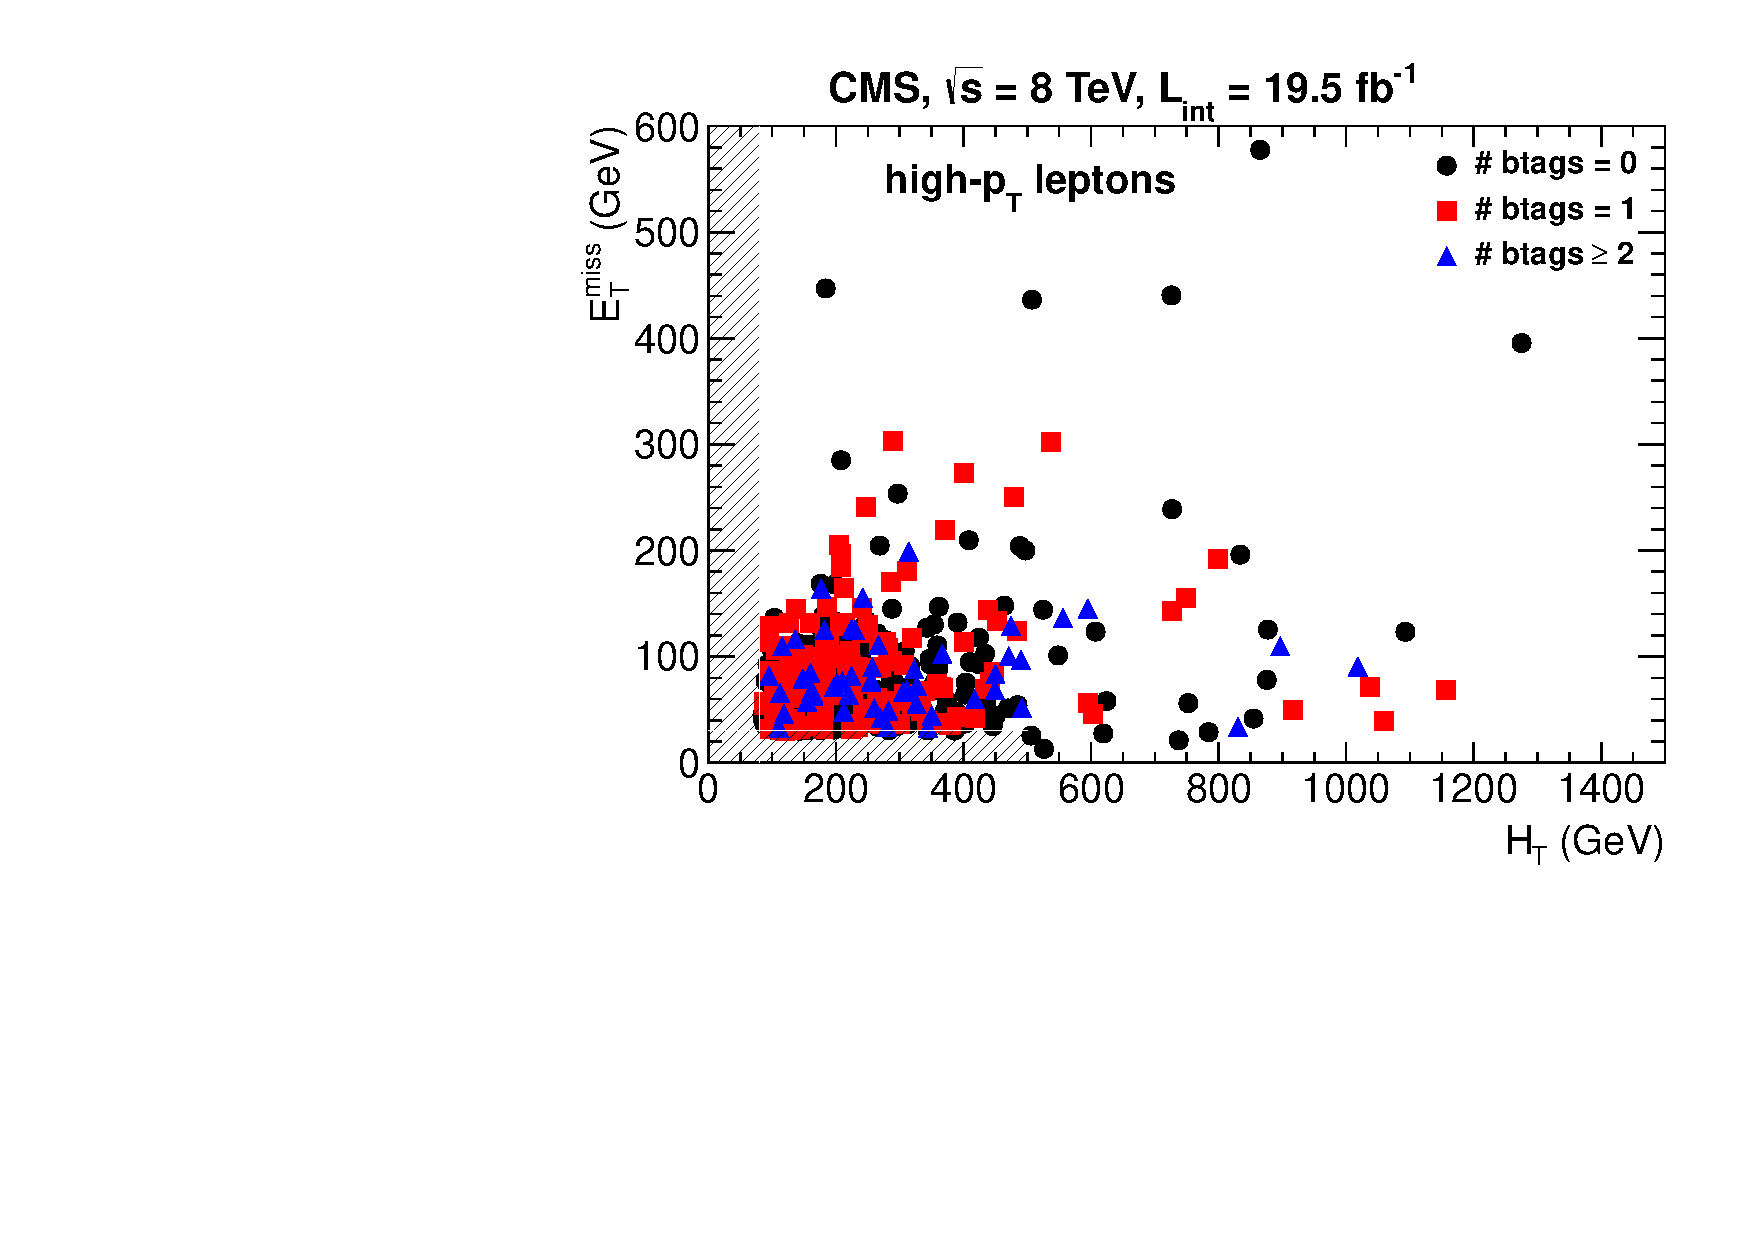
\includegraphics[width=0.8\linewidth]{p_ht_vs_met_hpt_sr0_nbs.pdf}
\end{center}
\caption[Distribution of events in the \Ht-\met plane passing the analysis selections for the \hpt baseline region]
{\label{fig:results_hpt_ht_vs_met}
Distribution of events in the \Ht-\met plane passing the analysis selections
for the \hpt baseline region (SR0).
}
\end{figure}

% --------------------------------------------------------------------------- %
The observed event yields and estimated backgrounds in the \hpt
control regions can be seen in Tables~\ref{tab:yield_excl_hpt_sr0},
\ref{tab:yield_excl_hpt_sr10}, and \ref{tab:yield_excl_hpt_sr20}. The yield
reported as {\it MC Pred} includes contributions from genuine same-sign lepton
pairs (sum of the rows from the \Wgamma down to the Higgs samples). The
statistical uncertainty on the simulated contributions is calculated using the
Clopper-Pearson method~\cite{clopperpearson}. Systematic uncertainties (the second uncertainty if
present) are displayed only for the final combined background component and no
uncertainty is added for estimates with zero entries. Systematic uncertainties
are 100\% correlated among the channels. The upper portion of the table (from
the top down to \ZZ) is based on simulation and is used as a reference only.
The total background when taken from simulation only is reported as {\it Total
MC} and again is given as a reference only. The SF (DF) contributions are for
events with one (two) fake leptons and the SC refers to the contamination to the
fake prediction from rare SM events.
% --------------------------------------------------------------------------- %
\begin{table}[!hbt]
\begin{center}
\caption[High \pt baseline yields and predictions with no b-tagged jets requirement (Signal Region 0)]
{\label{tab:yield_excl_hpt_sr0}\footnotesize{
\exclhptnamerZERO
\exclhptcutsrZERO
\exclcaption
}
}
\end{center} 
\resizebox{0.63\textwidth}{!}{\begin{minipage}{\textwidth}
\begin{tabular}{l|cccc} \hline\hline
source & $ee$ & $\mu\mu$ & $e\mu$ & $\ell\ell $ \\
\hline
$t\overline{t} \rightarrow \ell \ell X$ &  6.40 $\pm$  2.90 &  0.00 $\pm$  1.21 &  5.81 $\pm$  2.80 & 12.21 $\pm$  3.71 \\
$t\overline{t} \rightarrow \ell (b \rightarrow \ell) X$ & 13.86 $\pm$  3.98 & 10.25 $\pm$  3.56 & 22.25 $\pm$  4.78 & 46.36 $\pm$  6.65 \\
$t\overline{t} \rightarrow \ell (\slashed b \rightarrow \ell) X$ &  3.47 $\pm$  2.35 &  0.51 $\pm$  1.51 &  6.95 $\pm$  2.99 & 10.93 $\pm$  3.56 \\
        $t\overline{t}\ \rm{other}$ &  0.00 $\pm$  1.21 &  0.00 $\pm$  1.21 &  0.00 $\pm$  1.21 &  0.00 $\pm$  1.21 \\
\hline
                       t, s-channel &  0.00 $\pm$  0.52 &  0.00 $\pm$  0.52 &  0.00 $\pm$  0.52 &  0.00 $\pm$  0.52 \\
                       t, t-channel &  0.27 $\pm$  0.68 &  0.75 $\pm$  0.86 &  1.55 $\pm$  1.05 &  2.56 $\pm$  1.25 \\
                                 tW &  0.76 $\pm$  1.14 &  0.71 $\pm$  1.14 &  2.26 $\pm$  1.55 &  3.72 $\pm$  1.85 \\
\hline
         $DY \rightarrow \ell \ell$ & 18.03 $\pm$  9.25 &  0.00 $\pm$  4.14 &  5.81 $\pm$  6.57 & 23.85 $\pm$ 10.26 \\
      $W+jets \rightarrow \ell \nu$ &  0.00 $\pm$ 73.20 &  0.00 $\pm$ 73.20 &  0.00 $\pm$ 73.20 &  0.00 $\pm$ 73.20 \\
                                 WW &  0.00 $\pm$  0.11 &  0.00 $\pm$  0.11 &  0.00 $\pm$  0.11 &  0.00 $\pm$  0.11 \\
\hline
$W\gamma^{*} \rightarrow \ell \nu \mu\mu$ &  0.00 $\pm$  0.23 &  0.20 $\pm$  0.33 &  0.22 $\pm$  0.33 &  0.42 $\pm$  0.39 \\
$W\gamma^{*} \rightarrow \ell \nu \tau\tau$ &  0.11 $\pm$  0.30 &  0.22 $\pm$  0.34 &  0.00 $\pm$  0.24 &  0.33 $\pm$  0.38 \\
                                 WZ & 18.53 $\pm$  0.47 & 17.10 $\pm$  0.47 & 36.72 $\pm$  0.66 & 72.35 $\pm$  0.93 \\
                                 ZZ &  1.19 $\pm$  0.03 &  0.90 $\pm$  0.03 &  2.22 $\pm$  0.04 &  4.31 $\pm$  0.06 \\
\hline
              $t\overline{t}\gamma$ &  0.53 $\pm$  1.35 &  0.00 $\pm$  1.08 &  3.07 $\pm$  2.10 &  3.60 $\pm$  2.21 \\
                   $t\overline{t}W$ & 10.61 $\pm$  0.55 & 14.72 $\pm$  0.66 & 26.55 $\pm$  0.85 & 51.88 $\pm$  1.19 \\
                   $t\overline{t}Z$ &  2.80 $\pm$  0.26 &  3.16 $\pm$  0.29 &  6.25 $\pm$  0.39 & 12.20 $\pm$  0.54 \\
    $tbZ (Z \rightarrow \ell \ell)$ &  0.44 $\pm$  0.03 &  0.34 $\pm$  0.03 &  0.82 $\pm$  0.04 &  1.59 $\pm$  0.05 \\
                  $t\overline{t}WW$ &  0.22 $\pm$  0.01 &  0.29 $\pm$  0.01 &  0.51 $\pm$  0.01 &  1.01 $\pm$  0.01 \\
                         $WW\gamma$ &  0.00 $\pm$  0.09 &  0.00 $\pm$  0.09 &  0.00 $\pm$  0.09 &  0.00 $\pm$  0.09 \\
                                WWW &  1.84 $\pm$  0.13 &  2.44 $\pm$  0.15 &  4.17 $\pm$  0.19 &  8.45 $\pm$  0.27 \\
                                WWZ &  0.40 $\pm$  0.05 &  0.32 $\pm$  0.05 &  0.80 $\pm$  0.07 &  1.52 $\pm$  0.10 \\
                                WZZ &  0.08 $\pm$  0.01 &  0.08 $\pm$  0.01 &  0.19 $\pm$  0.02 &  0.36 $\pm$  0.03 \\
                                ZZZ &  0.01 $\pm$  0.00 &  0.00 $\pm$  0.00 &  0.01 $\pm$  0.00 &  0.02 $\pm$  0.00 \\
                 $qqW^{\pm}W^{\pm}$ &  8.07 $\pm$  0.66 & 11.04 $\pm$  0.79 & 20.11 $\pm$  1.01 & 39.22 $\pm$  1.40 \\
                            WW(DPS) &  0.10 $\pm$  0.06 &  0.19 $\pm$  0.07 &  0.31 $\pm$  0.08 &  0.60 $\pm$  0.11 \\
WH, ZH, $t\bar{t}H$; $H \rightarrow WW$ &  2.72 $\pm$  0.31 &  2.97 $\pm$  0.33 &  5.94 $\pm$  0.44 & 11.63 $\pm$  0.61 \\
WH, ZH, $t\bar{t}H$; $H \rightarrow ZZ$ &  0.12 $\pm$  0.01 &  0.15 $\pm$  0.02 &  0.29 $\pm$  0.02 &  0.55 $\pm$  0.03 \\
WH, ZH, $t\bar{t}H$; $H \rightarrow \tau\tau$ &  0.40 $\pm$  0.04 &  0.44 $\pm$  0.05 &  0.74 $\pm$  0.06 &  1.58 $\pm$  0.08 \\
\hline\hline
                           Total MC & 90.94 $\pm$ 74.03 & 66.77 $\pm$ 73.48 & 153.54 $\pm$ 73.85 & 311.24 $\pm$ 74.51 \\
\hline
                                 SF & 90.86 $\pm$  8.69 & 92.64 $\pm$  5.45 & 200.91 $\pm$ 11.00 & 384.41 $\pm$ 15.04 \\
                                 DF &  5.89 $\pm$  0.48 &  4.09 $\pm$  0.29 &  9.72 $\pm$  0.55 & 19.69 $\pm$  0.79 \\
                                 SC &  2.30 $\pm$  0.53 &  2.24 $\pm$  0.50 &  4.59 $\pm$  1.04 &  9.14 $\pm$  2.00 \\
                            SF + DF & 96.75 $\pm$  8.65 & 96.73 $\pm$  5.43 & 210.62 $\pm$ 10.96 & 404.10 $\pm$ 14.98 \\
\hline
                       SF + DF - SC & 94.44 $\pm$  8.66 $\pm$ 47.22 & 94.49 $\pm$  5.45 $\pm$ 47.24 & 206.03 $\pm$ 11.01 $\pm$ 103.02 & 394.96 $\pm$ 15.11 $\pm$ 197.48 \\
\hline\hline
                       Charge Flips & 23.44 $\pm$  1.16 $\pm$  7.03 &  0.00 $\pm$  0.00 $\pm$  0.00 &  5.22 $\pm$  0.45 $\pm$  1.57 & 28.66 $\pm$  1.24 $\pm$  8.60 \\
\hline
                            MC Pred & 48.15 $\pm$  1.77 $\pm$ 24.08 & 54.56 $\pm$  1.71 $\pm$ 27.28 & 108.91 $\pm$  2.68 $\pm$ 54.46 & 211.62 $\pm$  3.20 $\pm$ 105.81 \\
\hline
                         Total Pred & 166.04 $\pm$  8.92 $\pm$ 53.47 & 149.04 $\pm$  5.71 $\pm$ 54.55 & 320.17 $\pm$ 11.34 $\pm$ 116.53 & 635.24 $\pm$ 15.50 $\pm$ 224.21 \\
\hline\hline
                               Data &   146 &   111 &   220 &   477 \\
\hline\hline
\end{tabular}

 
\end{minipage} 
}
\end{table}
% --------------------------------------------------------------------------- %
\clearpage
% --------------------------------------------------------------------------- %
\begin{table}[!hbt]
\begin{center}
\caption[High \pt baseline yields and predictions with exaclty 1 b-tagged jet (Signal Region 10)]
{\label{tab:yield_excl_hpt_sr10}\footnotesize{
\exclhptnamerONEZERO
\exclhptcutsrONEZERO
\exclcaption
}
}
\end{center} 
\resizebox{0.65\textwidth}{!}{\begin{minipage}{\textwidth}
\begin{tabular}{l|cccc} \hline\hline
source & $ee$ & $\mu\mu$ & $e\mu$ & $\ell\ell $ \\
\hline
$t\overline{t} \rightarrow \ell \ell X$ &  3.51 $\pm$  2.35 &  0.00 $\pm$  1.21 &  3.47 $\pm$  2.35 &  6.99 $\pm$  2.99 \\
$t\overline{t} \rightarrow \ell (b \rightarrow \ell) X$ &  6.13 $\pm$  2.90 &  5.39 $\pm$  2.80 & 11.45 $\pm$  3.64 & 22.96 $\pm$  4.89 \\
$t\overline{t} \rightarrow \ell (\slashed b \rightarrow \ell) X$ &  1.70 $\pm$  1.91 &  0.51 $\pm$  1.51 &  4.06 $\pm$  2.47 &  6.27 $\pm$  2.90 \\
        $t\overline{t}\ \rm{other}$ &  0.00 $\pm$  1.21 &  0.00 $\pm$  1.21 &  0.00 $\pm$  1.21 &  0.00 $\pm$  1.21 \\
\hline
                       t, s-channel &  0.00 $\pm$  0.52 &  0.00 $\pm$  0.52 &  0.00 $\pm$  0.52 &  0.00 $\pm$  0.52 \\
                       t, t-channel &  0.27 $\pm$  0.68 &  0.26 $\pm$  0.68 &  0.53 $\pm$  0.77 &  1.06 $\pm$  0.93 \\
                                 tW &  0.37 $\pm$  1.00 &  0.00 $\pm$  0.80 &  1.87 $\pm$  1.46 &  2.24 $\pm$  1.55 \\
\hline
         $DY \rightarrow \ell \ell$ &  8.11 $\pm$  7.12 &  0.00 $\pm$  4.14 &  1.97 $\pm$  5.18 & 10.08 $\pm$  7.61 \\
      $W+jets \rightarrow \ell \nu$ &  0.00 $\pm$ 73.20 &  0.00 $\pm$ 73.20 &  0.00 $\pm$ 73.20 &  0.00 $\pm$ 73.20 \\
                                 WW &  0.00 $\pm$  0.11 &  0.00 $\pm$  0.11 &  0.00 $\pm$  0.11 &  0.00 $\pm$  0.11 \\
\hline
$W\gamma^{*} \rightarrow \ell \nu \mu\mu$ &  0.00 $\pm$  0.23 &  0.00 $\pm$  0.23 &  0.00 $\pm$  0.23 &  0.00 $\pm$  0.23 \\
$W\gamma^{*} \rightarrow \ell \nu \tau\tau$ &  0.00 $\pm$  0.24 &  0.00 $\pm$  0.24 &  0.00 $\pm$  0.24 &  0.00 $\pm$  0.24 \\
                                 WZ &  1.41 $\pm$  0.14 &  1.21 $\pm$  0.13 &  2.63 $\pm$  0.19 &  5.26 $\pm$  0.26 \\
                                 ZZ &  0.09 $\pm$  0.01 &  0.08 $\pm$  0.01 &  0.18 $\pm$  0.01 &  0.35 $\pm$  0.02 \\
\hline
              $t\overline{t}\gamma$ &  0.26 $\pm$  0.67 &  0.00 $\pm$  1.08 &  1.52 $\pm$  1.04 &  1.78 $\pm$  1.10 \\
                   $t\overline{t}W$ &  5.63 $\pm$  0.41 &  7.36 $\pm$  0.48 & 13.35 $\pm$  0.61 & 26.33 $\pm$  0.86 \\
                   $t\overline{t}Z$ &  1.53 $\pm$  0.20 &  1.69 $\pm$  0.22 &  2.96 $\pm$  0.27 &  6.17 $\pm$  0.39 \\
    $tbZ (Z \rightarrow \ell \ell)$ &  0.22 $\pm$  0.02 &  0.17 $\pm$  0.02 &  0.43 $\pm$  0.03 &  0.82 $\pm$  0.04 \\
                  $t\overline{t}WW$ &  0.10 $\pm$  0.00 &  0.15 $\pm$  0.01 &  0.25 $\pm$  0.01 &  0.49 $\pm$  0.01 \\
                         $WW\gamma$ &  0.00 $\pm$  0.09 &  0.00 $\pm$  0.09 &  0.00 $\pm$  0.09 &  0.00 $\pm$  0.09 \\
                                WWW &  0.15 $\pm$  0.04 &  0.22 $\pm$  0.05 &  0.37 $\pm$  0.06 &  0.74 $\pm$  0.09 \\
                                WWZ &  0.05 $\pm$  0.02 &  0.08 $\pm$  0.03 &  0.12 $\pm$  0.03 &  0.24 $\pm$  0.04 \\
                                WZZ &  0.01 $\pm$  0.01 &  0.01 $\pm$  0.01 &  0.03 $\pm$  0.01 &  0.05 $\pm$  0.01 \\
                                ZZZ &  0.00 $\pm$  0.00 &  0.00 $\pm$  0.00 &  0.00 $\pm$  0.00 &  0.00 $\pm$  0.00 \\
                 $qqW^{\pm}W^{\pm}$ &  0.44 $\pm$  0.20 &  1.04 $\pm$  0.28 &  1.48 $\pm$  0.31 &  2.96 $\pm$  0.42 \\
                            WW(DPS) &  0.01 $\pm$  0.03 &  0.00 $\pm$  0.03 &  0.04 $\pm$  0.04 &  0.05 $\pm$  0.04 \\
WH, ZH, $t\bar{t}H$; $H \rightarrow WW$ &  1.34 $\pm$  0.22 &  1.12 $\pm$  0.21 &  2.89 $\pm$  0.31 &  5.35 $\pm$  0.42 \\
WH, ZH, $t\bar{t}H$; $H \rightarrow ZZ$ &  0.05 $\pm$  0.01 &  0.05 $\pm$  0.01 &  0.09 $\pm$  0.01 &  0.18 $\pm$  0.02 \\
WH, ZH, $t\bar{t}H$; $H \rightarrow \tau\tau$ &  0.11 $\pm$  0.02 &  0.13 $\pm$  0.03 &  0.24 $\pm$  0.03 &  0.48 $\pm$  0.05 \\
\hline\hline
                           Total MC & 31.49 $\pm$ 73.70 & 19.46 $\pm$ 73.43 & 49.92 $\pm$ 73.60 & 100.86 $\pm$ 73.93 \\
\hline
                                 SF & 41.00 $\pm$  4.36 & 45.33 $\pm$  3.19 & 91.84 $\pm$  5.69 & 178.17 $\pm$  7.84 \\
                                 DF &  1.53 $\pm$  0.23 &  1.57 $\pm$  0.17 &  2.97 $\pm$  0.28 &  6.07 $\pm$  0.40 \\
                                 SC &  0.65 $\pm$  0.19 &  0.56 $\pm$  0.16 &  1.14 $\pm$  0.29 &  2.35 $\pm$  0.59 \\
                            SF + DF & 42.53 $\pm$  4.34 & 46.90 $\pm$  3.17 & 94.81 $\pm$  5.67 & 184.24 $\pm$  7.81 \\
\hline
                       SF + DF - SC & 41.88 $\pm$  4.35 $\pm$ 20.94 & 46.34 $\pm$  3.18 $\pm$ 23.17 & 93.66 $\pm$  5.67 $\pm$ 46.83 & 181.89 $\pm$  7.83 $\pm$ 90.94 \\
\hline\hline
                       Charge Flips &  4.00 $\pm$  0.22 $\pm$  1.20 &  0.00 $\pm$  0.00 $\pm$  0.00 &  2.52 $\pm$  0.22 $\pm$  0.76 &  6.53 $\pm$  0.31 $\pm$  1.96 \\
\hline
                            MC Pred & 11.40 $\pm$  0.94 $\pm$  5.70 & 13.30 $\pm$  1.31 $\pm$  6.65 & 26.57 $\pm$  1.38 $\pm$ 13.29 & 51.27 $\pm$  1.63 $\pm$ 25.63 \\
\hline
                         Total Pred & 57.28 $\pm$  4.45 $\pm$ 21.74 & 59.64 $\pm$  3.43 $\pm$ 24.11 & 122.76 $\pm$  5.84 $\pm$ 48.69 & 239.68 $\pm$  8.01 $\pm$ 94.51 \\
\hline\hline
                               Data &    42 &    35 &    75 &   152 \\
\hline\hline
\end{tabular}


\end{minipage} 
}
\end{table}
% --------------------------------------------------------------------------- %
\clearpage
% --------------------------------------------------------------------------- %
\begin{table}[!hbt]
\begin{center}
\caption[High \pt baseline yields and predictions with two or more b-tagged jets (Signal Region 20)]
{\label{tab:yield_excl_hpt_sr20}\footnotesize{
\exclhptnamerTWOZERO
\exclhptcutsrTWOZERO
\exclcaption
}
}
\end{center} 
\resizebox{0.67\textwidth}{!}{\begin{minipage}{\textwidth}
\begin{tabular}{l|cccc} \hline\hline
source & $ee$ & $\mu\mu$ & $e\mu$ & $\ell\ell $ \\
\hline
$t\overline{t} \rightarrow \ell \ell X$ &  1.16 $\pm$  1.73 &  0.00 $\pm$  1.21 &  1.74 $\pm$  1.91 &  2.89 $\pm$  2.22 \\
$t\overline{t} \rightarrow \ell (b \rightarrow \ell) X$ &  0.00 $\pm$  1.21 &  0.56 $\pm$  1.51 &  2.26 $\pm$  2.07 &  2.81 $\pm$  2.22 \\
$t\overline{t} \rightarrow \ell (\slashed b \rightarrow \ell) X$ &  1.16 $\pm$  1.73 &  0.00 $\pm$  1.21 &  0.00 $\pm$  1.21 &  1.16 $\pm$  1.73 \\
        $t\overline{t}\ \rm{other}$ &  0.00 $\pm$  1.21 &  0.00 $\pm$  1.21 &  0.00 $\pm$  1.21 &  0.00 $\pm$  1.21 \\
\hline
                       t, s-channel &  0.00 $\pm$  0.52 &  0.00 $\pm$  0.52 &  0.00 $\pm$  0.52 &  0.00 $\pm$  0.52 \\
                       t, t-channel &  0.00 $\pm$  0.54 &  0.00 $\pm$  0.54 &  0.77 $\pm$  0.86 &  0.77 $\pm$  0.86 \\
                                 tW &  0.00 $\pm$  0.80 &  0.00 $\pm$  0.80 &  0.00 $\pm$  0.80 &  0.00 $\pm$  0.80 \\
\hline
         $DY \rightarrow \ell \ell$ &  0.00 $\pm$  4.14 &  0.00 $\pm$  4.14 &  0.00 $\pm$  4.14 &  0.00 $\pm$  4.14 \\
      $W+jets \rightarrow \ell \nu$ &  0.00 $\pm$ 73.20 &  0.00 $\pm$ 73.20 &  0.00 $\pm$ 73.20 &  0.00 $\pm$ 73.20 \\
                                 WW &  0.00 $\pm$  0.11 &  0.00 $\pm$  0.11 &  0.00 $\pm$  0.11 &  0.00 $\pm$  0.11 \\
\hline
$W\gamma^{*} \rightarrow \ell \nu \mu\mu$ &  0.00 $\pm$  0.23 &  0.00 $\pm$  0.23 &  0.00 $\pm$  0.23 &  0.00 $\pm$  0.23 \\
$W\gamma^{*} \rightarrow \ell \nu \tau\tau$ &  0.00 $\pm$  0.24 &  0.00 $\pm$  0.24 &  0.00 $\pm$  0.24 &  0.00 $\pm$  0.24 \\
                                 WZ &  0.04 $\pm$  0.03 &  0.08 $\pm$  0.04 &  0.15 $\pm$  0.05 &  0.26 $\pm$  0.07 \\
                                 ZZ &  0.01 $\pm$  0.00 &  0.01 $\pm$  0.00 &  0.01 $\pm$  0.00 &  0.02 $\pm$  0.01 \\
\hline
              $t\overline{t}\gamma$ &  0.15 $\pm$  0.37 &  0.00 $\pm$  1.08 &  0.85 $\pm$  0.58 &  0.99 $\pm$  0.61 \\
                   $t\overline{t}W$ &  2.73 $\pm$  0.29 &  3.80 $\pm$  0.35 &  7.20 $\pm$  0.46 & 13.73 $\pm$  0.63 \\
                   $t\overline{t}Z$ &  0.70 $\pm$  0.14 &  0.69 $\pm$  0.15 &  1.78 $\pm$  0.22 &  3.17 $\pm$  0.28 \\
    $tbZ (Z \rightarrow \ell \ell)$ &  0.05 $\pm$  0.01 &  0.05 $\pm$  0.01 &  0.10 $\pm$  0.01 &  0.19 $\pm$  0.02 \\
                  $t\overline{t}WW$ &  0.06 $\pm$  0.00 &  0.07 $\pm$  0.00 &  0.14 $\pm$  0.01 &  0.27 $\pm$  0.01 \\
                         $WW\gamma$ &  0.00 $\pm$  0.09 &  0.00 $\pm$  0.09 &  0.00 $\pm$  0.09 &  0.00 $\pm$  0.09 \\
                                WWW &  0.01 $\pm$  0.02 &  0.02 $\pm$  0.02 &  0.04 $\pm$  0.03 &  0.07 $\pm$  0.03 \\
                                WWZ &  0.00 $\pm$  0.01 &  0.00 $\pm$  0.01 &  0.01 $\pm$  0.01 &  0.02 $\pm$  0.02 \\
                                WZZ &  0.01 $\pm$  0.00 &  0.00 $\pm$  0.00 &  0.01 $\pm$  0.00 &  0.01 $\pm$  0.01 \\
                                ZZZ &  0.00 $\pm$  0.00 &  0.00 $\pm$  0.00 &  0.00 $\pm$  0.00 &  0.00 $\pm$  0.00 \\
                 $qqW^{\pm}W^{\pm}$ &  0.00 $\pm$  0.09 &  0.03 $\pm$  0.05 &  0.07 $\pm$  0.12 &  0.10 $\pm$  0.12 \\
                            WW(DPS) &  0.00 $\pm$  0.03 &  0.00 $\pm$  0.03 &  0.00 $\pm$  0.03 &  0.00 $\pm$  0.03 \\
WH, ZH, $t\bar{t}H$; $H \rightarrow WW$ &  0.55 $\pm$  0.15 &  0.70 $\pm$  0.17 &  0.95 $\pm$  0.19 &  2.20 $\pm$  0.28 \\
WH, ZH, $t\bar{t}H$; $H \rightarrow ZZ$ &  0.02 $\pm$  0.01 &  0.03 $\pm$  0.01 &  0.06 $\pm$  0.01 &  0.12 $\pm$  0.01 \\
WH, ZH, $t\bar{t}H$; $H \rightarrow \tau\tau$ &  0.05 $\pm$  0.02 &  0.06 $\pm$  0.02 &  0.10 $\pm$  0.02 &  0.21 $\pm$  0.03 \\
\hline\hline
                           Total MC &  6.69 $\pm$ 73.39 &  6.09 $\pm$ 73.38 & 16.23 $\pm$ 73.41 & 29.02 $\pm$ 73.44 \\
\hline
                                 SF &  5.05 $\pm$  1.05 &  5.05 $\pm$  0.87 & 12.40 $\pm$  1.54 & 22.50 $\pm$  2.06 \\
                                 DF &  0.20 $\pm$  0.08 &  0.28 $\pm$  0.07 &  0.25 $\pm$  0.07 &  0.73 $\pm$  0.13 \\
                                 SC &  0.30 $\pm$  0.10 &  0.24 $\pm$  0.08 &  0.50 $\pm$  0.17 &  1.05 $\pm$  0.32 \\
                            SF + DF &  5.25 $\pm$  1.04 &  5.33 $\pm$  0.86 & 12.65 $\pm$  1.53 & 23.23 $\pm$  2.04 \\
\hline
                       SF + DF - SC &  4.95 $\pm$  1.04 $\pm$  2.48 &  5.09 $\pm$  0.87 $\pm$  2.54 & 12.15 $\pm$  1.54 $\pm$  6.07 & 22.18 $\pm$  2.07 $\pm$ 11.09 \\
\hline\hline
                       Charge Flips &  1.41 $\pm$  0.09 $\pm$  0.42 &  0.00 $\pm$  0.00 $\pm$  0.00 &  1.42 $\pm$  0.12 $\pm$  0.43 &  2.83 $\pm$  0.15 $\pm$  0.85 \\
\hline
                            MC Pred &  4.37 $\pm$  0.63 $\pm$  2.19 &  5.54 $\pm$  1.21 $\pm$  2.77 & 11.47 $\pm$  0.88 $\pm$  5.73 & 21.38 $\pm$  1.03 $\pm$ 10.69 \\
\hline
                         Total Pred & 10.74 $\pm$  1.22 $\pm$  3.33 & 10.62 $\pm$  1.49 $\pm$  3.76 & 25.03 $\pm$  1.78 $\pm$  8.36 & 46.39 $\pm$  2.32 $\pm$ 15.43 \\
\hline\hline
                               Data &    11 &    16 &    25 &    52 \\
\hline\hline
\end{tabular}


\end{minipage} 
}
\end{table}
% --------------------------------------------------------------------------- %
\clearpage

Consider first the inclusive baseline SR0. Simulation alone indicates an expected
background contribution of 20\% fake leptons, 10\% leptons with incorrect
charge assignment and 70\% from SM source is prompt, isolated same-sign
dileptons.  This is in contrast to previous iterations of this analysis which
saw the contribution from fake leptons dominating the background composition.
This is due to the tighter impact parameter requirement on the lepton selection
and increased yield of the rare process with the increase in both luminosity
and center-of-mass energy of the collisions. The background from fake leptons
is mostly from top events. It is difficult to estimate the contribution from
\Wj due to the limited statistics in this sample with a large uncertainty of
$\pm72$ events; but this could be a significant component of the fake lepton
background. The background from electrons with a mis-reconstructed charge comes
from fully leptonic \ttbar decays and \DY events. The remaining irreducible
background comes from several different process that involve genuine same-sign
dileptons, although most predominately are \ttW, \WZ, and \qqWW.

The data-driven background estimation over-predicts by a factor of almost
seven higher than that expected from pure simulation ($\approx 63$ vs.
395). This is attributed to several factors. First, the fake rate
method itself over-predicted by 60\% in the \ttbar closure test shown in
Section~\ref{sec:bkgd_fakes_frstudy_closure}. This accounts for the 50\%
systematic uncertainty driven by this method. Secondly, the simulation also
has a large uncertainty since the \Wj sample has low statistics. Finally,
the simulation itself may be failing to accurately account for all the sources
of fake leptons. When one accounts for the large uncertainties on both the
simulated and data-driven fake lepton prediction, the methods are
consistent and thus no correction is made at this time.

In baselines SR10 and SR20, a b-tagged jet requirement is made. This reduces
the contributions from rare SM processes such as \WZ and \qqWW where
there are no intrinsic b-quarks in the final state. In these regions, the
contributions from fakes leptons becomes reduced due to the increased b-tagged
jet requirement. Figure~\ref{fig:results_yield_hpt_bl} shows a graphical
representation of the yields and there full background predictions for SR0,
SR10 and SR20. Here we see the background prediction and the data yield are in
agreement within the uncertainty. This lends confidence that our data-driven
methods are performing reasonably well.

% --------------------------------------------------------------------------- %
\begin{figure}[h]
\begin{center}
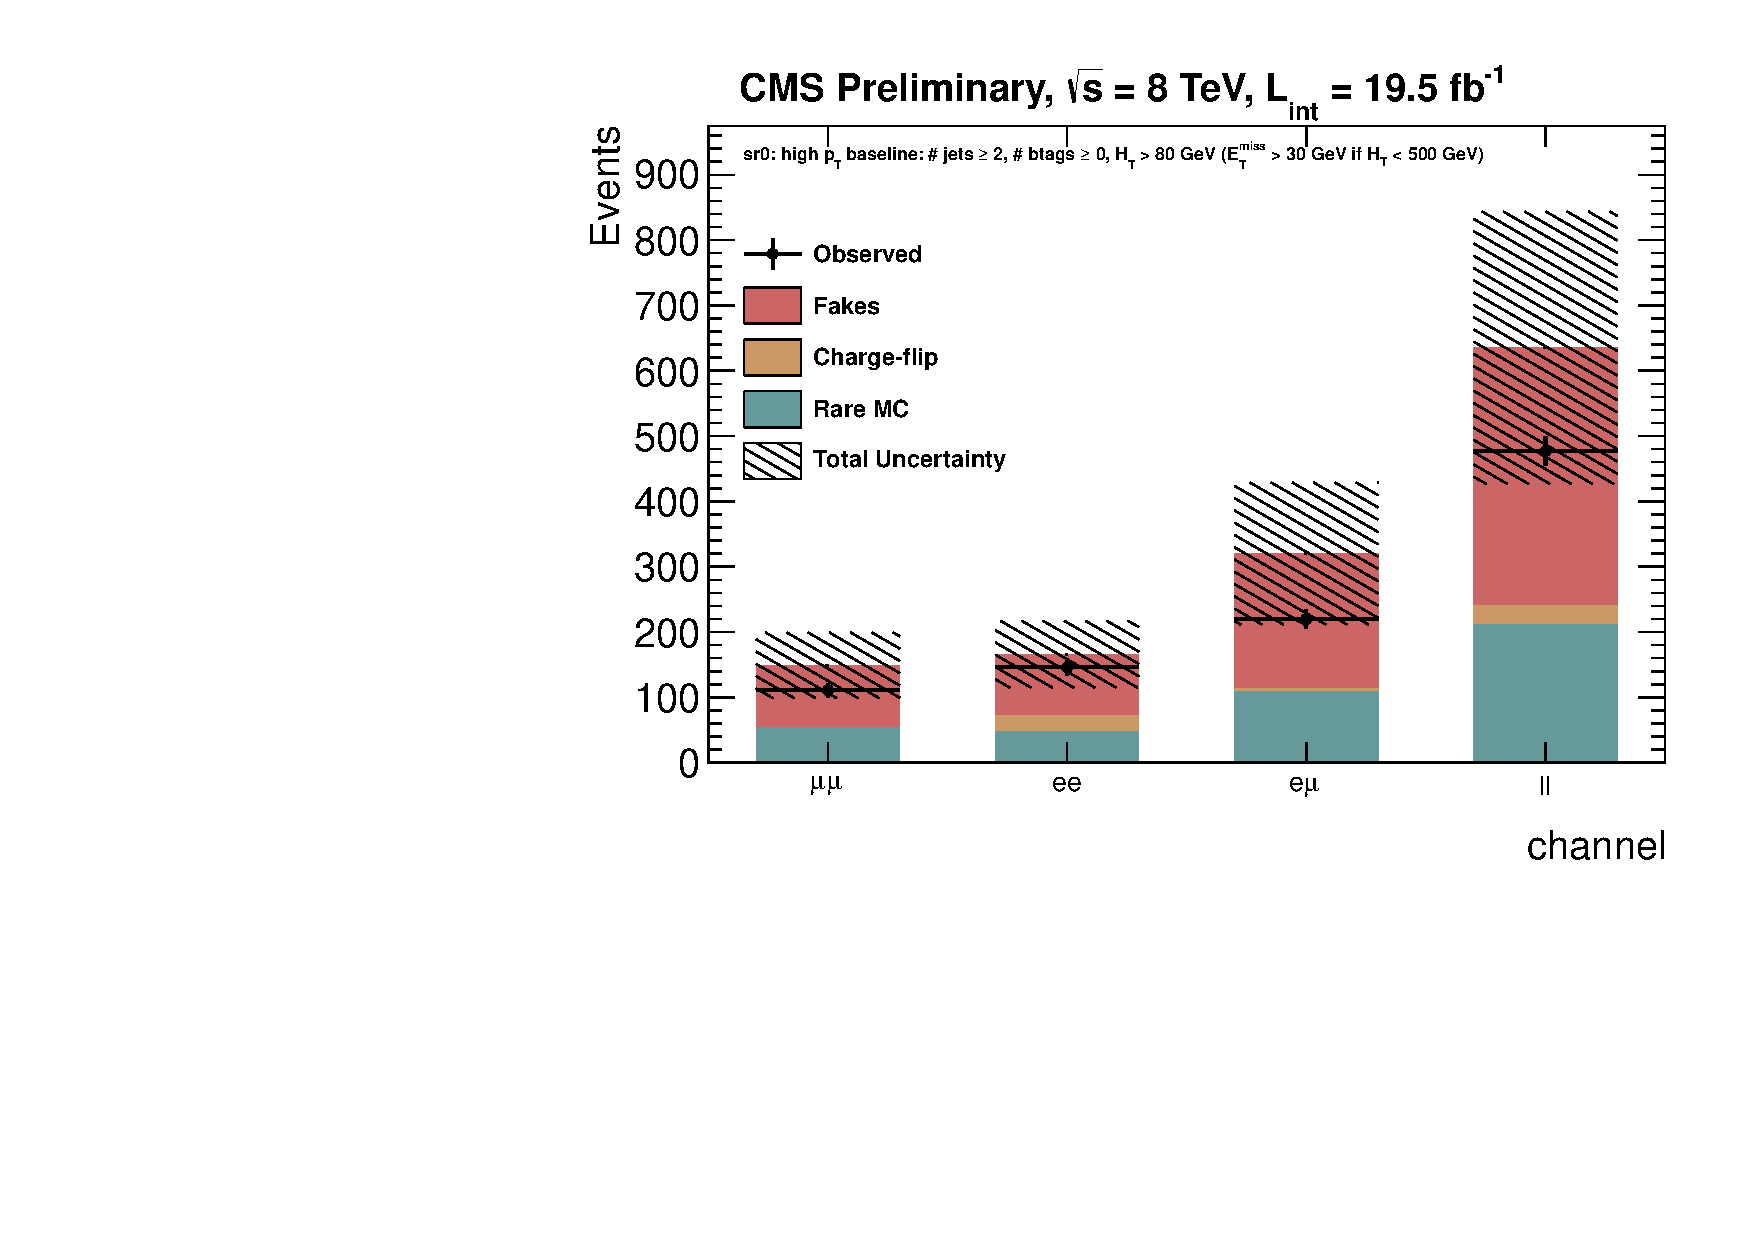
\includegraphics[width=0.49\linewidth]{p_hpt_sr0_yield}
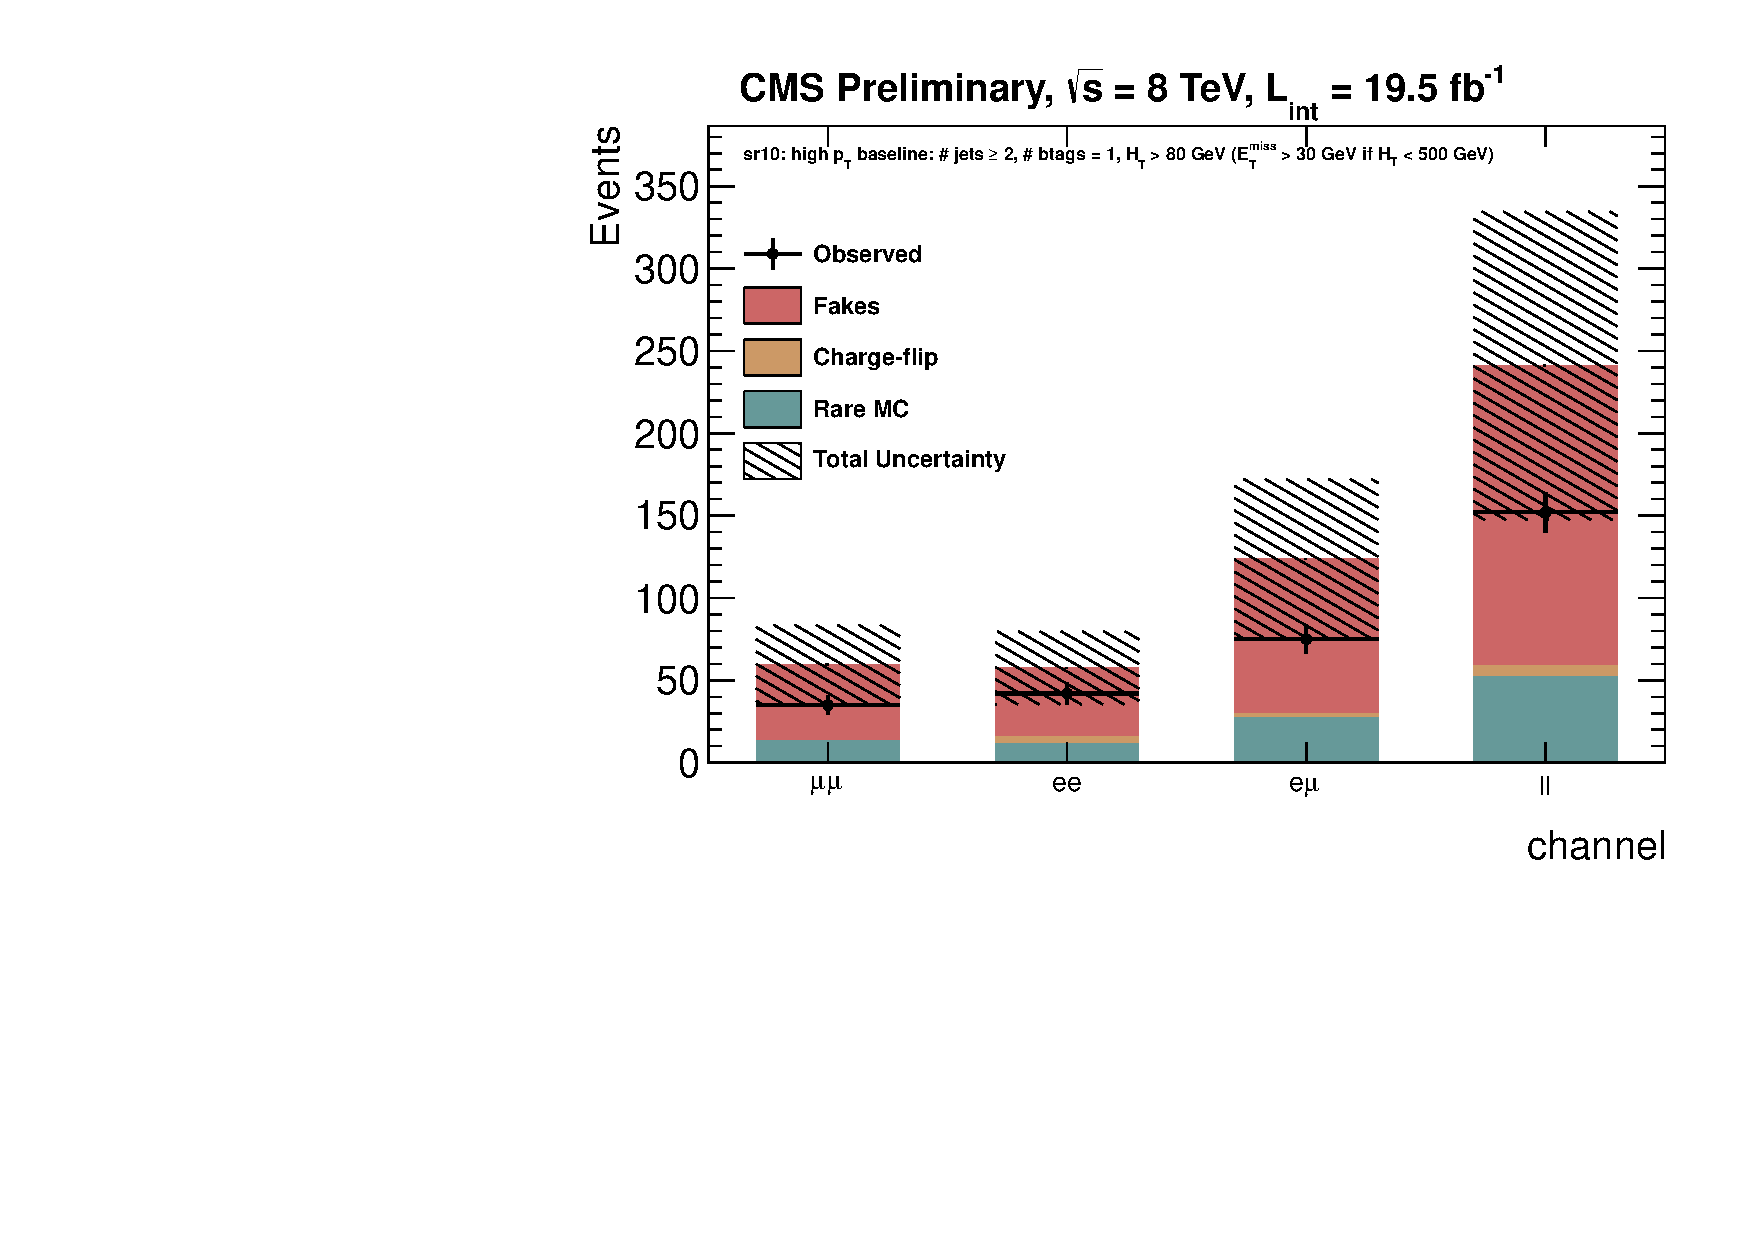
\includegraphics[width=0.49\linewidth]{p_hpt_sr10_yield}
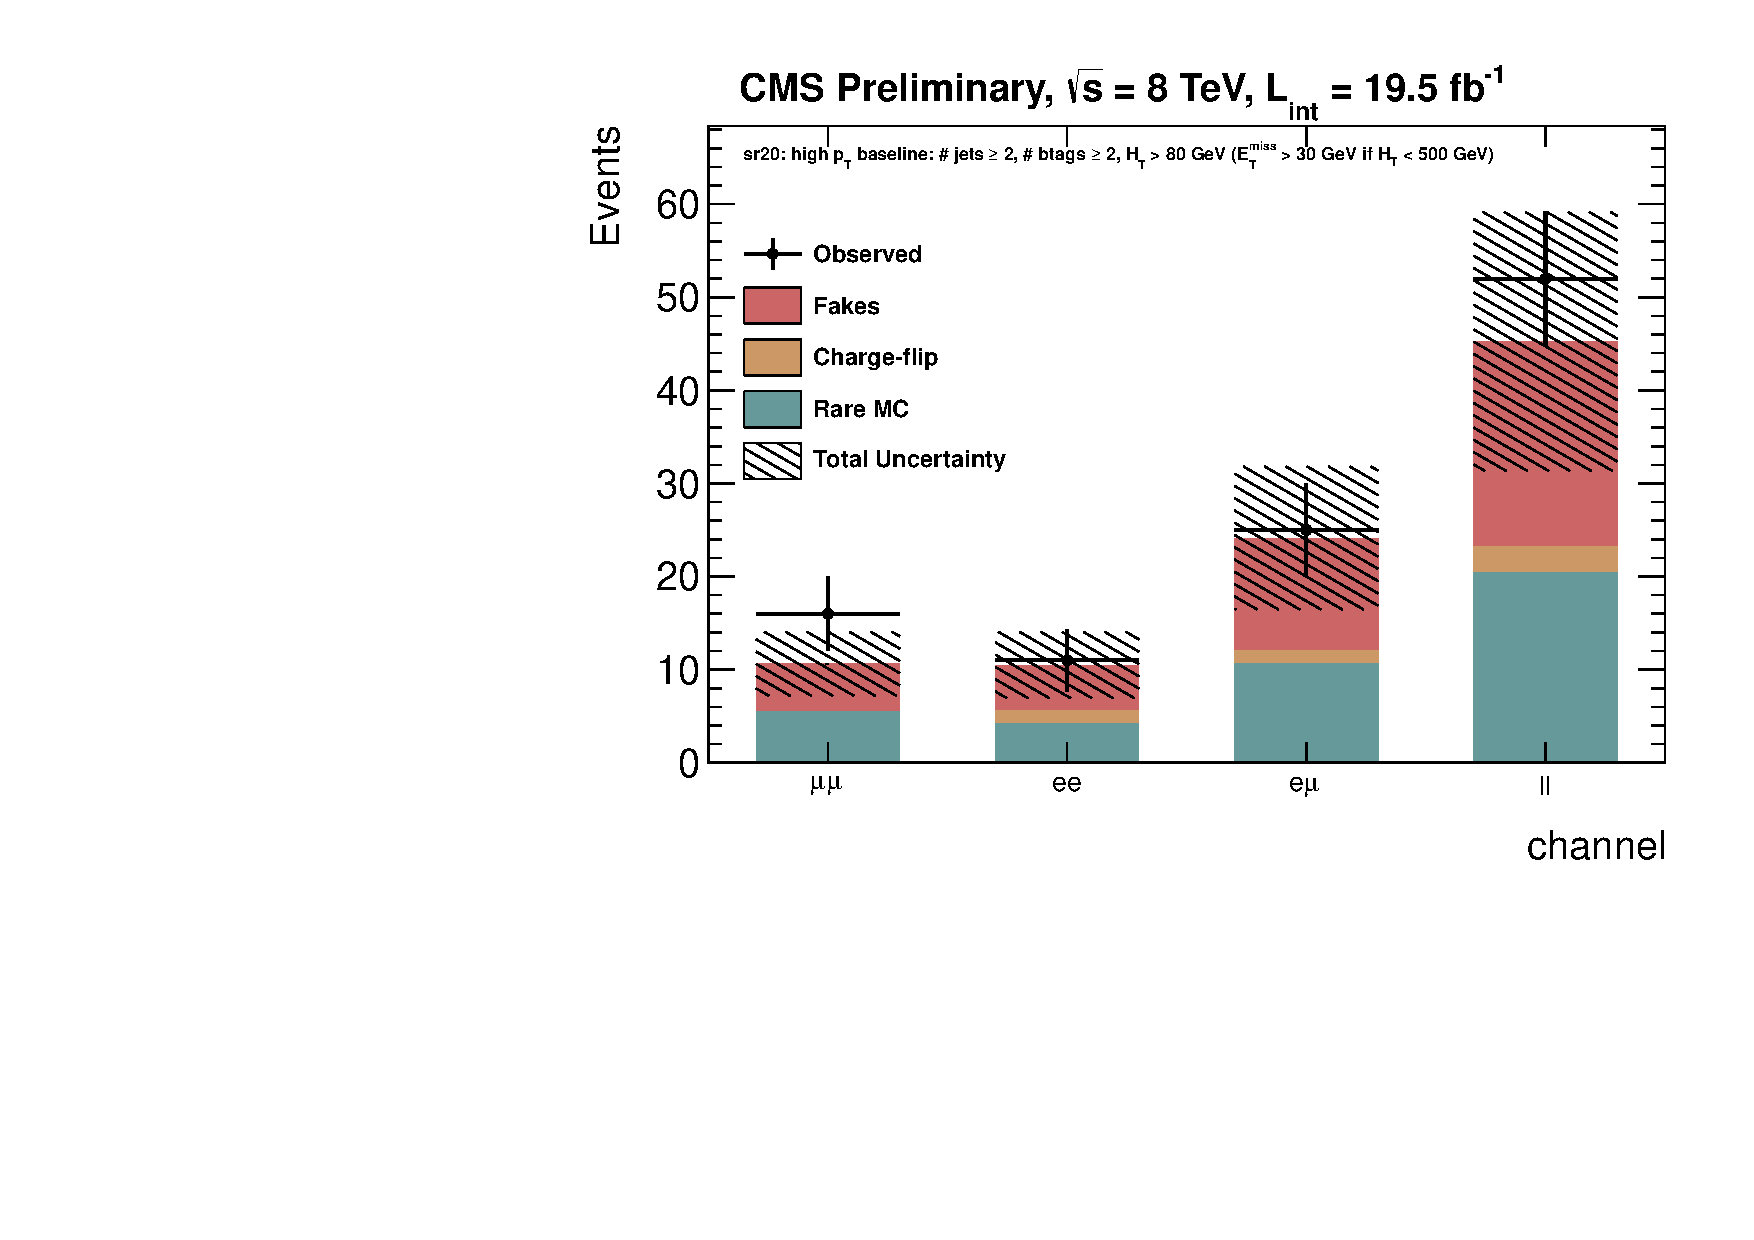
\includegraphics[width=0.49\linewidth]{p_hpt_sr20_yield}
\caption[Graphical representation of the event yields in the \hpt baseline regions]
{\label{fig:results_yield_hpt_bl}
Graphical representation of the event yields in the \hpt baseline region
with no (top left), exactly one (top right) and $\geq 2$ (bottom column)
\nbtags~requirement (Search Region 0, 10 and 20). Also shown as a histogram
is the result of the background prediction. The shading around the histogram
represents the uncertainty in the background prediction.
}
\end{center}
\end{figure}
% --------------------------------------------------------------------------- %
\clearpage
% --------------------------------------------------------------------------- %
% --------------------------------------------------------------------------- %
\subsection{High \pt Search Regions}
\label {sec:results_hpt_sr}
% --------------------------------------------------------------------------- %

We now consider the search regions shown in Table~\ref{tab:evtsel_sr_hpt}
and repeated in Table~\ref{tab:results_sr_hpt} for convenience. The
observed yields and estimated backgrounds for each region are shown in
Table~\ref{tab:results_hpt_excl_yield_summary}. The uncertainty is the total
statistical and systematic uncertainty. A graphical representation of these
results can also be seen in Figure~\ref{fig:results_yield_hpt_sr}. We see no
evidence of an event yield in significant excess of the background estimations.
% --------------------------------------------------------------------------- %
\begin{table}[!htb]
\begin{center}
\caption[Search regions selected for the high \pt~analysis]
{\label{tab:results_sr_hpt}
Search regions selected for the high \pt~search where we require $\Ht>200\ \GeV$.
}
\begin{tabular}{c|c|c|c|c}
\hline\hline
\nbtags                   & \met                    & \njets   & \Ht[200-400] & \Ht[$>400$] \\ \hline
\multirow{4}{*}{$=0$}     & \multirow{2}{*}{50-120} & 2-3      & SR1          & SR2         \\ \cline{3-5}
                          &                         & $\geq 4$ & SR3          & SR4         \\ \cline{2-5}
                          & \multirow{2}{*}{$>120$} & 2-3      & SR5          & SR6         \\ \cline{3-5}
                          &                         & $\geq 4$ & SR7          & SR8         \\ \hline
\multirow{4}{*}{$=1$}     & \multirow{2}{*}{50-120} & 2-3      & SR11         & SR12        \\ \cline{3-5}
                          &                         & $\geq 4$ & SR13         & SR14        \\ \cline{2-5}
                          & \multirow{2}{*}{$>120$} & 2-3      & SR15         & SR16        \\ \cline{3-5}
                          &                         & $\geq 4$ & SR17         & SR18        \\ \hline
\multirow{4}{*}{$\geq 2$} & \multirow{2}{*}{50-120} & 2-3      & SR21         & SR22        \\ \cline{3-5}
                          &                         & $\geq 4$ & SR23         & SR24        \\ \cline{2-5}
                          & \multirow{2}{*}{$>120$} & 2-3      & SR25         & SR26        \\ \cline{3-5}
                          &                         & $\geq 4$ & SR27         & SR28        \\ \hline\hline
\end{tabular}
\end{center}
\end{table}

% --------------------------------------------------------------------------- %
\begin{table}
\begin{center}
\caption[A summary of the results of this search for the \hpt~analysis]
{\label{tab:results_hpt_excl_yield_summary}
A summary of the results of this search for the \hpt~analysis. For each signal
region, we show its most important kinematical requirements, the prediction for
the three background (BG) components as well as the total, and the event yield.
} 
\end{center}
\resizebox{0.58\textwidth}{!}{\begin{minipage}{\textwidth}
\begin{tabular}{|c|c|c|c|c|c|c|c|c|c|}
\hline
\nbtags                   & \met                    & \njets                    & \Ht     & SR & Fake BG           & Flip BG        & Rare MC           & Total BG          & Observed \\ \hline\hline
$\geq 0$                  & 30 if $\Ht<500$ else 0  & 2                         & 80      & 0  & 394.96$\pm$198.06 & 28.66$\pm$8.69 & 211.62$\pm$105.86 & 635.24$\pm$224.74 & 477      \\ \hline
\multirow{8}{*}{$= 0$}    & \multirow{4}{*}{50-120} & \multirow{2}{*}{2-3}      & 200-400 & 1  & 28.62$\pm$14.52   & 1.56$\pm$0.48  & 25.84$\pm$12.96   & 56.02$\pm$19.47   & 48       \\ \cline{4-5}
                          &                         &                           & $>400$  & 2  & 2.94$\pm$1.63     & 0.37$\pm$0.12  & 6.30$\pm$3.20     & 9.61$\pm$3.60     & 11       \\ \cline{3-5}
                          &                         & \multirow{2}{*}{$\geq 4$} & 200-400 & 3  & 5.64$\pm$2.98     & 0.13$\pm$0.04  & 2.54$\pm$1.36     & 8.32$\pm$3.28     & 5        \\ \cline{4-5}
                          &                         &                           & $>400$  & 4  & 2.33$\pm$1.33     & 0.15$\pm$0.05  & 2.99$\pm$1.58     & 5.47$\pm$2.07     & 2        \\ \cline{2-5}
                          & \multirow{4}{*}{$>120$} & \multirow{2}{*}{2-3}      & 200-400 & 5  & 8.53$\pm$4.45     & 0.19$\pm$0.06  & 12.74$\pm$6.41    & 21.47$\pm$7.81    & 12       \\ \cline{4-5}
                          &                         &                           & $>400$  & 6  & 2.11$\pm$1.23     & 0.06$\pm$0.02  & 7.38$\pm$3.75     & 9.55$\pm$3.94     & 11       \\ \cline{3-5}
                          &                         & \multirow{2}{*}{$\geq 4$} & 200-400 & 7  & 1.32$\pm$0.81     & 0.02$\pm$0.01  & 0.87$\pm$0.60     & 2.21$\pm$1.01     & 1        \\ \cline{4-5}
                          &                         &                           & $>400$  & 8  & 1.97$\pm$1.13     & 0.02$\pm$0.01  & 2.41$\pm$1.29     & 4.40$\pm$1.72     & 3        \\ \hline
\multirow{9}{*}{$=1$}     & 30 if $\Ht<500$ else 0  & 2                         & 80      & 10 & 181.89$\pm$91.28  & 6.53$\pm$1.98  & 51.27$\pm$25.69   & 239.68$\pm$94.85  & 152      \\ \cline{2-5}
                          & \multirow{4}{*}{50-120} & \multirow{2}{*}{2-3}      & 200-400 & 11 & 34.63$\pm$17.51   & 1.00$\pm$0.31  & 9.13$\pm$4.61     & 44.76$\pm$18.10   & 29       \\ \cline{4-5}
                          &                         &                           & $>400$  & 12 & 1.88$\pm$1.10     & 0.12$\pm$0.04  & 2.01$\pm$1.10     & 4.01$\pm$1.56     & 5        \\ \cline{3-5}
                          &                         & \multirow{2}{*}{$\geq 4$} & 200-400 & 13 & 7.00$\pm$3.67     & 0.16$\pm$0.05  & 3.73$\pm$1.93     & 10.89$\pm$4.15    & 6        \\ \cline{4-5}
                          &                         &                           & $>400$  & 14 & 4.27$\pm$2.31     & 0.09$\pm$0.03  & 3.00$\pm$1.57     & 7.35$\pm$2.79     & 2        \\ \cline{2-5}
                          & \multirow{4}{*}{$>120$} & \multirow{2}{*}{2-3}      & 200-400 & 15 & 6.31$\pm$3.31     & 0.33$\pm$0.10  & 4.91$\pm$2.51     & 11.55$\pm$4.16    & 11       \\ \cline{4-5}
                          &                         &                           & $>400$  & 16 & 1.70$\pm$1.02     & 0.07$\pm$0.02  & 2.33$\pm$1.25     & 4.10$\pm$1.62     & 2        \\ \cline{3-5}
                          &                         & \multirow{2}{*}{$\geq 4$} & 200-400 & 17 & 2.03$\pm$1.16     & 0.04$\pm$0.01  & 1.24$\pm$0.75     & 3.31$\pm$1.38     & 3        \\ \cline{4-5}
                          &                         &                           & $>400$  & 18 & 1.27$\pm$0.78     & 0.05$\pm$0.02  & 2.45$\pm$1.30     & 3.76$\pm$1.52     & 7        \\ \hline
\multirow{9}{*}{$\geq 2$} & 30 if $\Ht<500$ else 0  & 2                         & 80      & 20 & 22.18$\pm$11.28   & 2.83$\pm$0.86  & 21.38$\pm$10.74   & 46.39$\pm$15.60   & 52       \\ \cline{2-5}
                          & \multirow{4}{*}{50-120} & \multirow{2}{*}{2-3}      & 200-400 & 21 & 3.87$\pm$2.10     & 0.56$\pm$0.17  & 4.00$\pm$2.06     & 8.43$\pm$2.95     & 12       \\ \cline{4-5}
                          &                         &                           & $>400$  & 22 & 0.28$\pm$0.26     & 0.06$\pm$0.02  & 0.69$\pm$0.52     & 1.03$\pm$0.59     & 1        \\ \cline{3-5}
                          &                         & \multirow{2}{*}{$\geq 4$} & 200-400 & 23 & 2.40$\pm$1.35     & 0.11$\pm$0.04  & 2.10$\pm$1.14     & 4.61$\pm$1.77     & 3        \\ \cline{4-5}
                          &                         &                           & $>400$  & 24 & 1.13$\pm$0.72     & 0.06$\pm$0.02  & 2.03$\pm$1.11     & 3.23$\pm$1.32     & 7        \\ \cline{2-5}
                          & \multirow{4}{*}{$>120$} & \multirow{2}{*}{2-3}      & 200-400 & 25 & 0.99$\pm$0.63     & 0.14$\pm$0.04  & 1.81$\pm$1.00     & 2.94$\pm$1.19     & 4        \\ \cline{4-5}
                          &                         &                           & $>400$  & 26 & 0.13$\pm$0.19     & 0.03$\pm$0.01  & 0.76$\pm$0.54     & 0.91$\pm$0.58     & 1        \\ \cline{3-5}
                          &                         & \multirow{2}{*}{$\geq 4$} & 200-400 & 27 & 0.38$\pm$0.34     & 0.03$\pm$0.01  & 0.73$\pm$0.54     & 1.14$\pm$0.64     & 0        \\ \cline{4-5}
                          &                         &                           & $>400$  & 28 & 0.45$\pm$0.34     & 0.03$\pm$0.01  & 1.67$\pm$0.94     & 2.16$\pm$1.00     & 2        \\ \hline
\end{tabular}
\end{minipage}
}
\end{table}
% --------------------------------------------------------------------------- %

% --------------------------------------------------------------------------- %
\begin{figure}[h]
\begin{center}
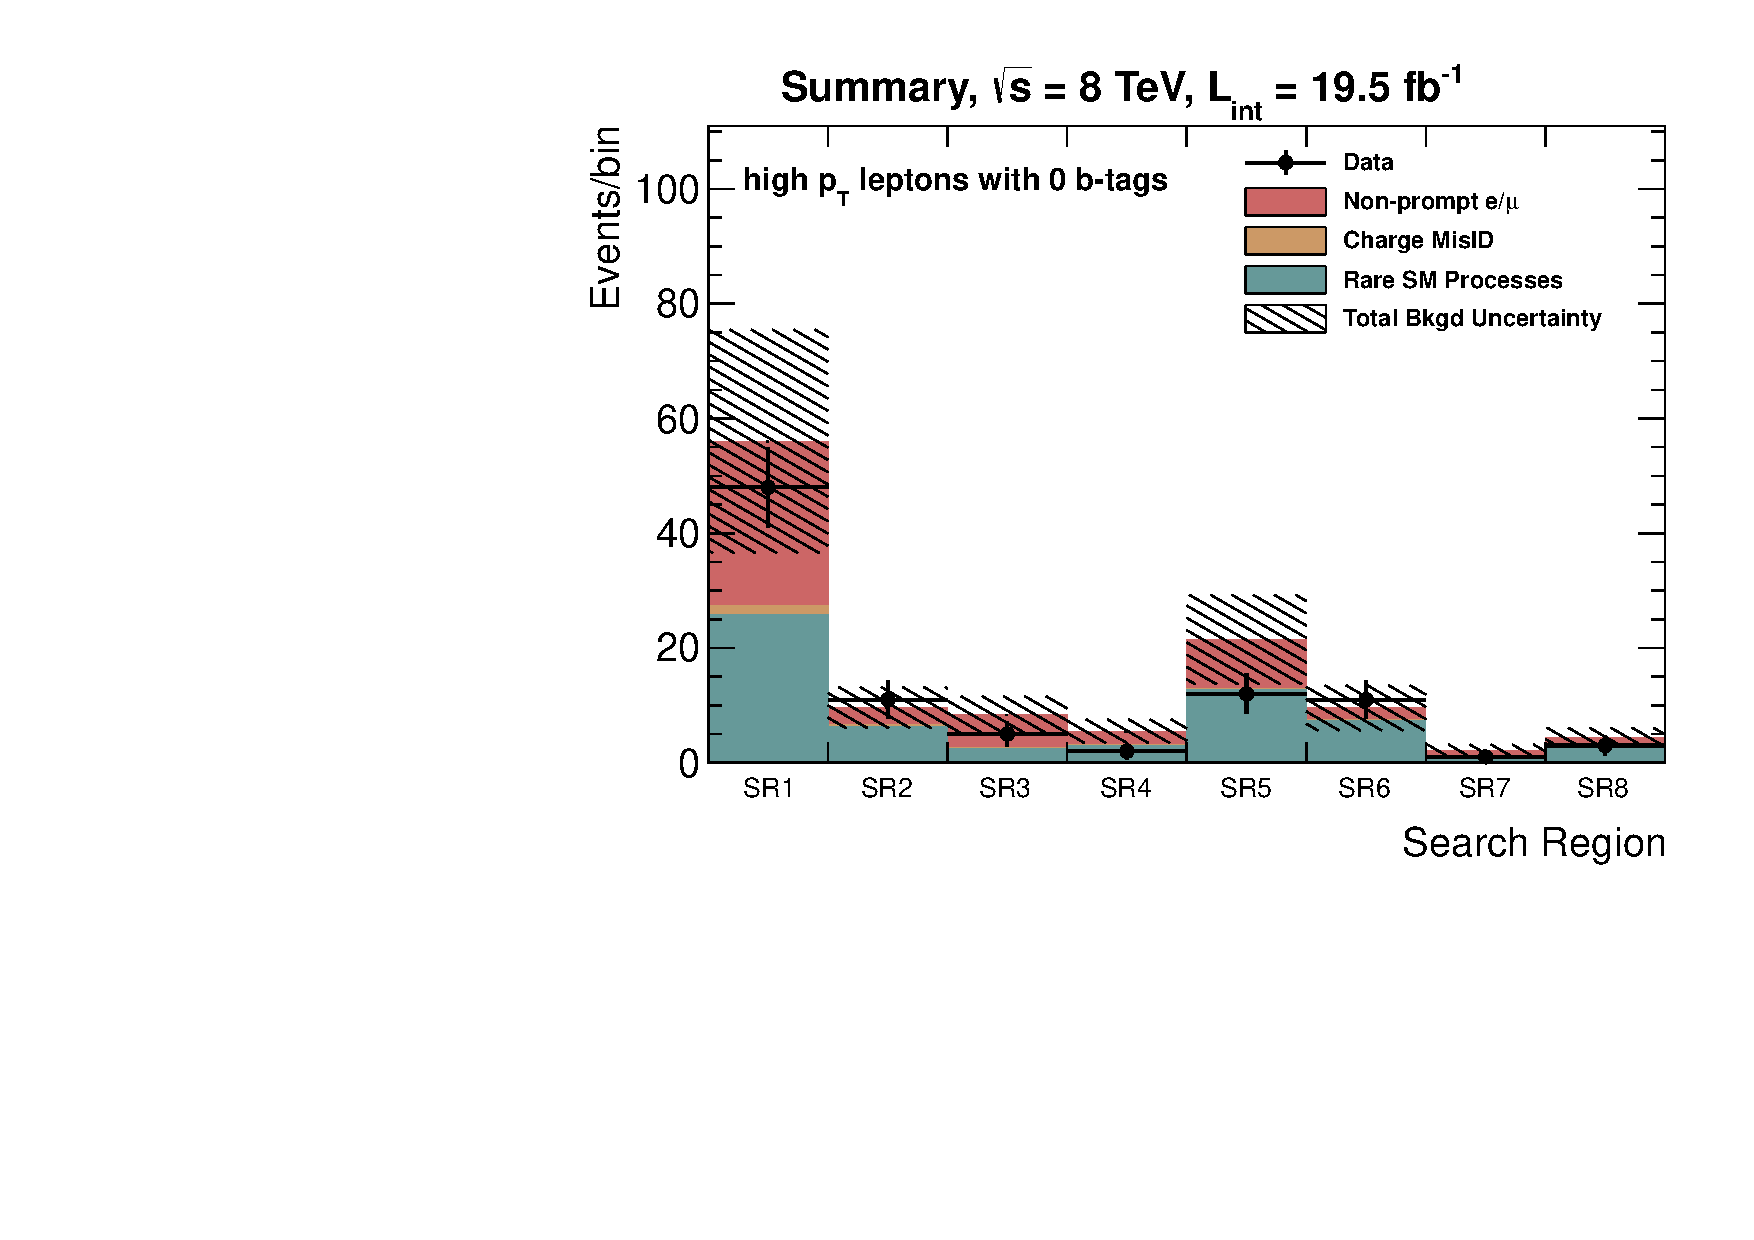
\includegraphics[width=0.49\linewidth]{p_yields_hpt_exclusive_nb0}
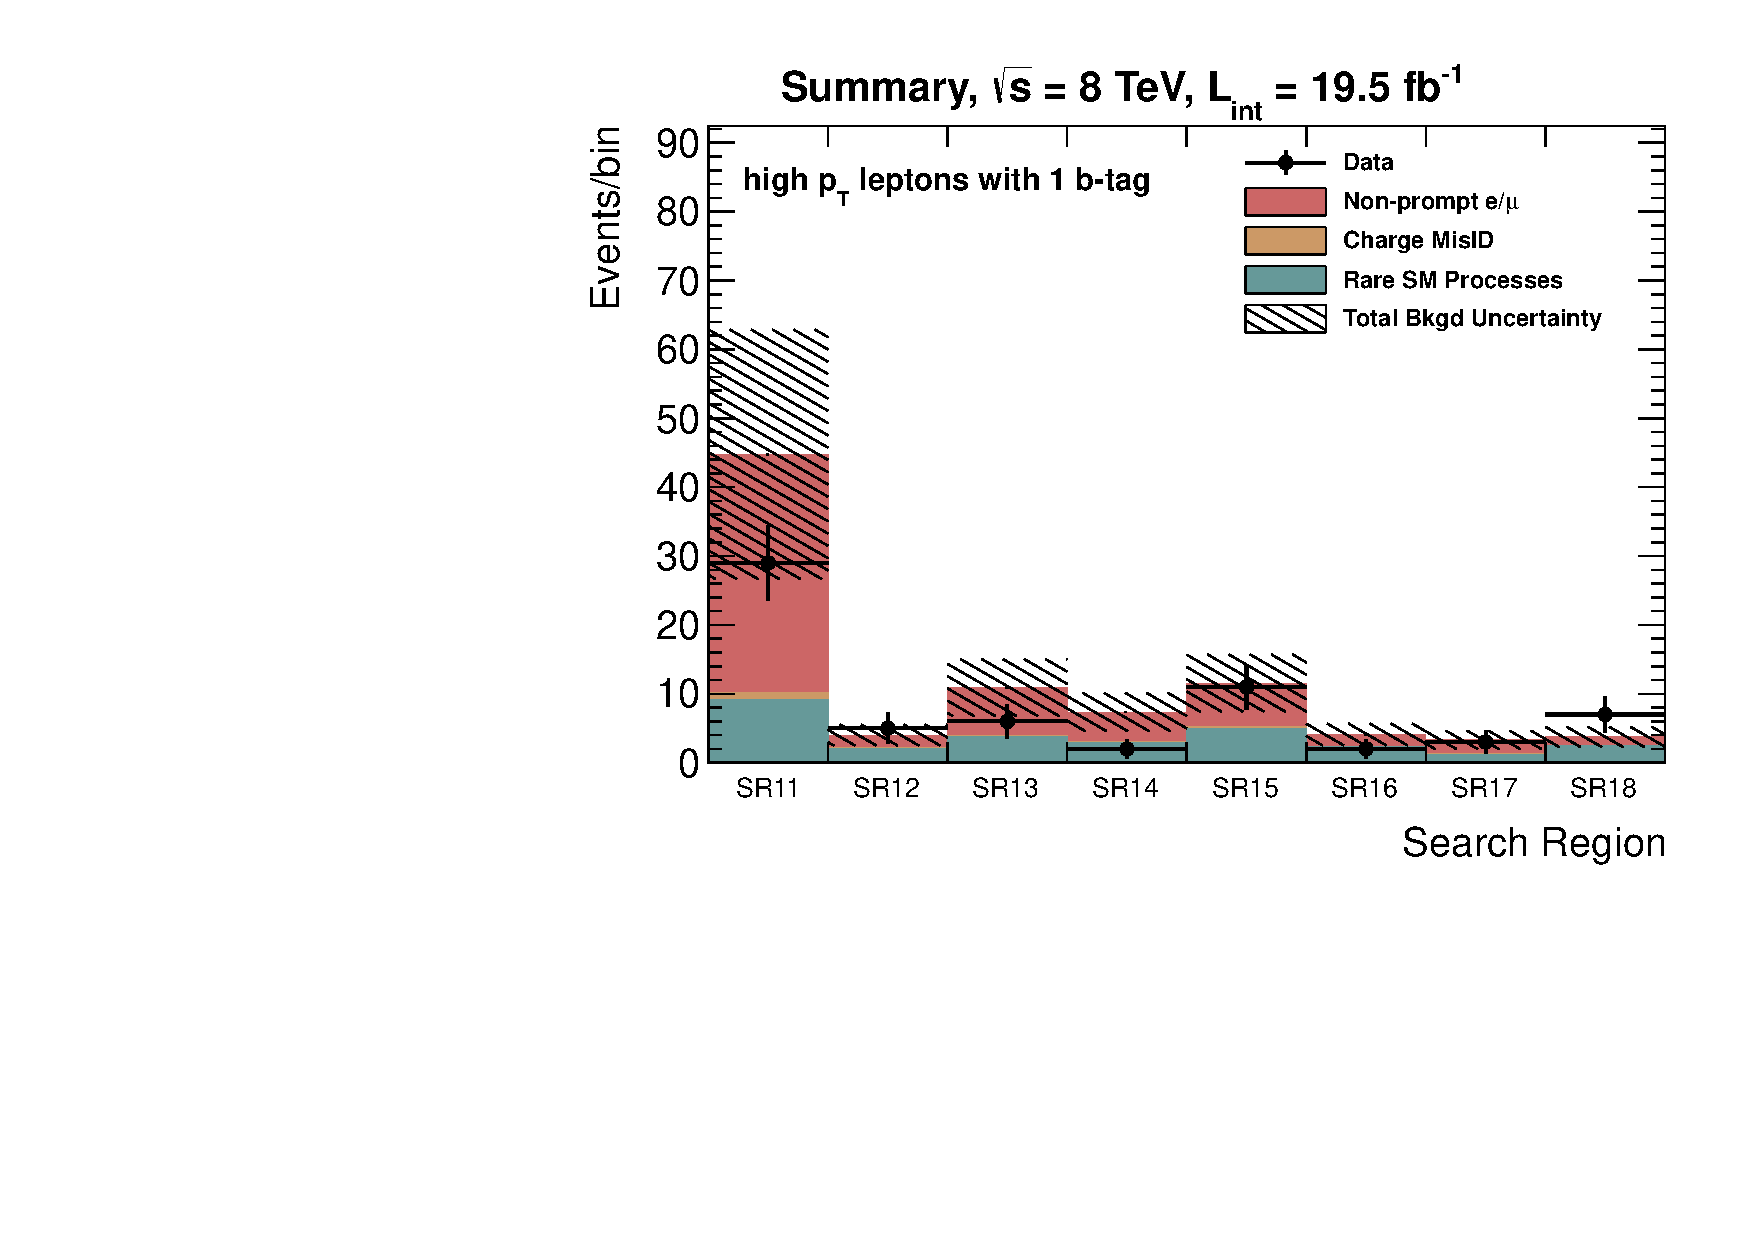
\includegraphics[width=0.49\linewidth]{p_yields_hpt_exclusive_nb1}
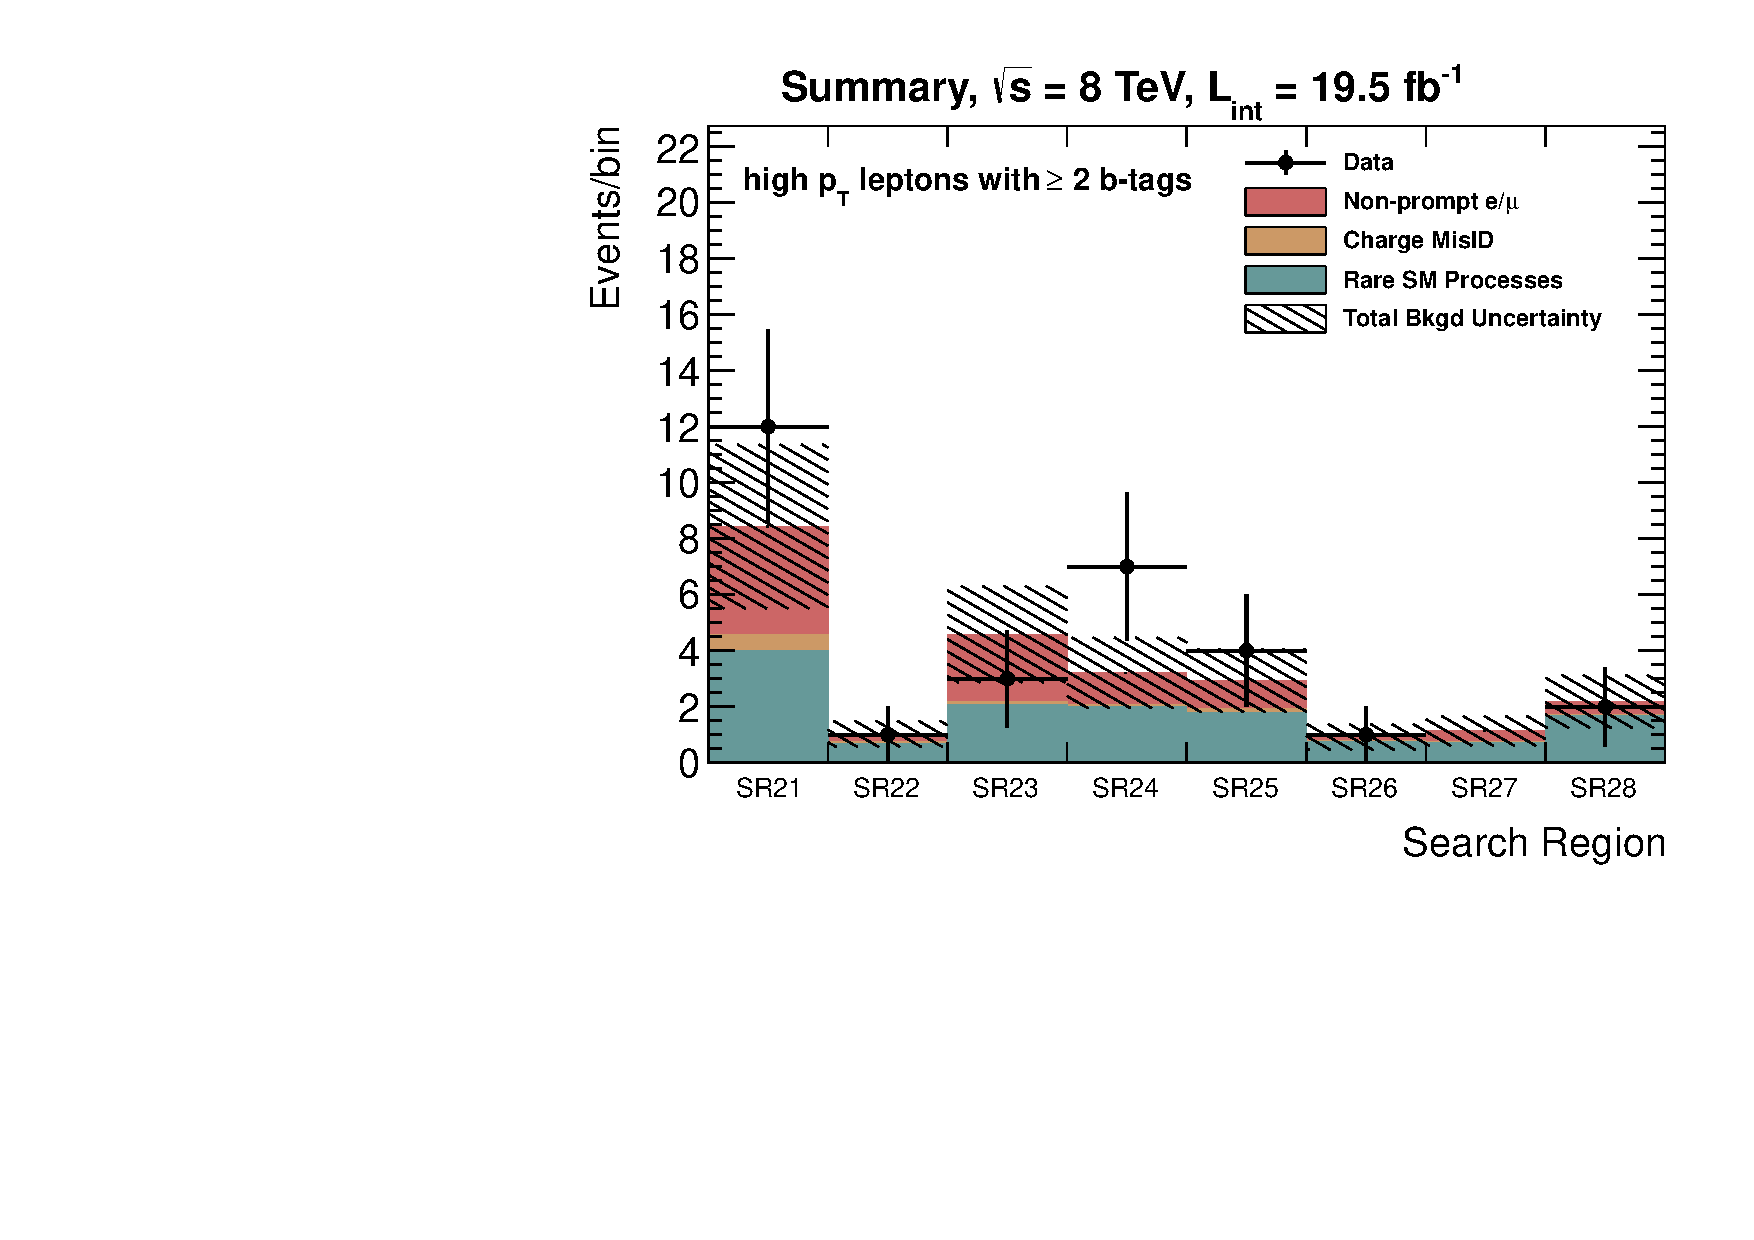
\includegraphics[width=0.49\linewidth]{p_yields_hpt_exclusive_nb2}
\caption[Graphical representation of the event yields in the \hpt search regions]
{\label{fig:results_yield_hpt_sr}
Graphical representation of the event yields in the \hpt search regions
with one (top left), exactly one (top right) and $\geq 2$ (bottom column)
\nbtags~requirement (Search Region 1-8, 11-18, and 21-28). Also shown as a histogram
is the result of the background prediction. The shading around the histogram
represents the uncertainty in the background prediction.
}
\end{center}
\end{figure}

% --------------------------------------------------------------------------- %
In the various search regions, irreducible backgrounds, primarily from \ttW,
\WZ and \qqWW, are the dominant backgrounds at approximately 25-80\%, depending
on the search region. Fake leptons account for approximately 15-75\% of the
background also depending on the search region. The background from charge
mis-reconstruction is small contributing less than 5\%.

% --------------------------------------------------------------------------- %
% --------------------------------------------------------------------------- %
\section{Low \pt Results}
\label {sec:results_lpt}
% --------------------------------------------------------------------------- %
% --------------------------------------------------------------------------- %

% --------------------------------------------------------------------------- %
\subsection{Low \pt Control Regions}
\label {sec:results_lpt_bl}
% --------------------------------------------------------------------------- %

For the \lpt analysis, the control region (baseline) selections were
listed in Table~\ref{tab:evtsel_srbl} but are repeated here for convenience in
Table~\ref{tab:results_srbl_lpt}.
% --------------------------------------------------------------------------- %
\begin{table}[!tbh]
\begin{center}
\caption[Summary of the baseline search regions considered in the \lpt analysis]
{\label{tab:results_srbl_lpt}
Summary of the baseline search regions considered in the \lpt analysis.
}
\end{center}
\resizebox{0.78\textwidth}{!}{\begin{minipage}{\textwidth}
\begin{tabular}{c|c|c|c|c|c}
\hline\hline
Search Region \# & min lepton \pt ($\mu$, e) (\GeV) & \Ht (\GeV)           & \met (\GeV)                               & \njets             & \nbtags \\ \hline
SR0              & \multirow{3}{*}{10, 10}          & \multirow{3}{*}{250} & \multirow{3}{*}{30 if $\Ht < 500$ else 0} & \multirow{3}{*}{2} & $\ge$ 0 \\ \cline{1-1}\cline{6-6}
SR10             &                                  &                      &                                           &                    & = 1     \\ \cline{1-1}\cline{6-6}
SR20             &                                  &                      &                                           &                    & $\ge$ 2 \\ \hline\hline
\end{tabular}
\end{minipage}
}
\end{table}  
% --------------------------------------------------------------------------- %
The control regions in the \lpt analysis are essentially the same as the \hpt
analysis with two notable exceptions: the lepton \pt threshold is lowered from
20 to 10 \GeV on both leptons and the minimum \Ht requirement is raised from
80 to 250 \GeV. The lowered lepton \pt allows more sensitivity for regions
with a compressed mass spectrum that would lead to lower \pt leptons. The
\Ht requirement is raised since the low \pt online trigger selection has a
minimum \Ht requirement of 175 \GeV; thus, 250 \GeV was chosen to account for
the trigger turn-on. As with the \hpt analysis, the control region SR0 was
designed to be inclusive to all the search regions and is mostly sensitive
to fake leptons in SM multi-jet processes: predominately \ttbar and \Wj. The
contribution for backgrounds without intrinsic b-quarks is suppressed in SR10
and SR20 which add a \nbtags requirement of exactly one and at least two,
respectively. Figure~\ref{fig:results_lpt_ht_vs_met} shows the distribution of
events from SR0 in the \Ht-\met plane. The events cluster in lower left corner
as expected for background events.

% --------------------------------------------------------------------------- %
\begin{figure}[!htb]
\begin{center}
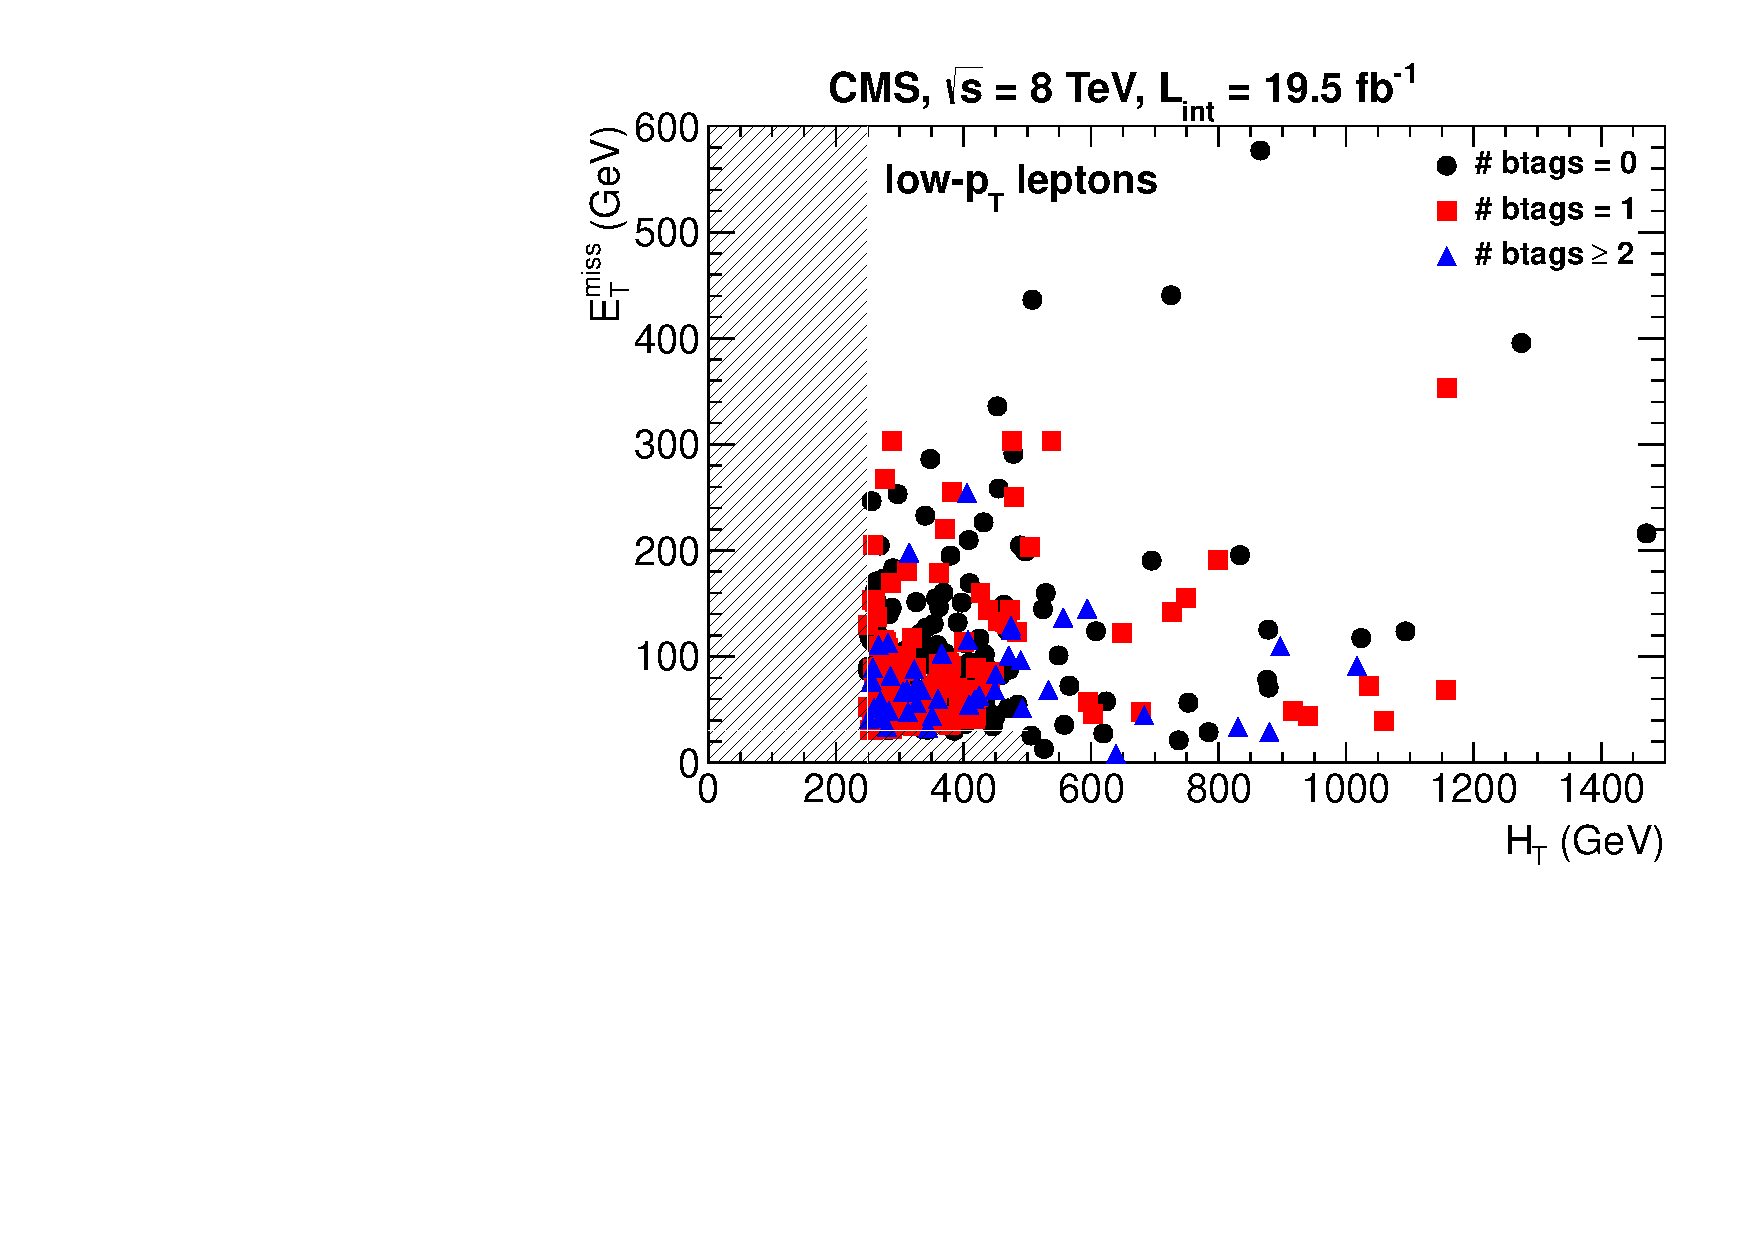
\includegraphics[width=0.8\linewidth]{p_ht_vs_met_lpt_sr0_nbs.pdf}
\end{center}
\caption[Distribution of events in the \Ht-\met plane passing the analysis selections for the \lpt baseline region]
{\label{fig:results_lpt_ht_vs_met}
Distribution of events in the \Ht-\met plane passing the analysis selections
for the \lpt baseline region (SR0).
}
\end{figure}
% --------------------------------------------------------------------------- %

The observed event yields and estimated backgrounds in the \lpt
control regions can be seen in Tables~\ref{tab:yield_excl_lpt_sr0},
\ref{tab:yield_excl_lpt_sr10}, and \ref{tab:yield_excl_lpt_sr20}. The yield
reported as {\it MC Pred} includes contributions from genuine same-sign lepton
pairs (sum of the rows from the \Wgamma down to the Higgs samples). The
statistical uncertainty on the simulated contributions is calculated using the
Clopper-Pearson method~\cite{clopperpearson}. Systematic uncertainties (the second uncertainty if
present) are displayed only for the final combined background component and no
uncertainty is added for estimates with zero entries. Systematic uncertainties
are 100\% correlated among the channels. The upper portion of the table (from
the top down to \ZZ) is based on simulation only and is used as a reference only.
The total background when taken from simulation only is reported as {\it Total
MC} and again is given as a reference only. The SF(DF) contributions are for
events with one(two) fake leptons and the SC refers to the contamination to the
fake prediction from rare SM events.

The data-driven background estimation over-predicts by a factor of almost
four higher than that expected from pure simulation ($\approx 73$ vs.
240). This is attributed to several factors. First, the fake rate
method itself over-predicted by 60\% in the \ttbar closure test shown in
Section~\ref{sec:bkgd_fakes_frstudy_closure}. This accounts for the 50\%
systematic uncertainty driven by this method. Secondly, the simulation also
has a large uncertainty since the \Wj sample has low statistics. Finally,
the simulation itself may be failing to accurately account for all the sources
of fake leptons. When one accounts for the large uncertainties on both the
simulated and data-driven fake lepton prediction, the methods are
consistent and thus no correction is made at this time.

Consider first the inclusive baseline SR0. Simulation alone indicates a that
background contribution of 20\% fake leptons, 10\% leptons with incorrect
charge assignment and 70\% from SM source is prompt, isolated same-sign
dileptons. The background from fake leptons is mostly from top events. Its
difficult to estimate the contribution from \Wj due to the limited statistics
in this sample with a large uncertainty of $\pm72$ events; but this could be
a significant component of the fake lepton background. The background from
electrons with a mis-reconstructed charge comes from fully leptonic \ttbar
decays and \DY events. The remaining irreducible background comes from several
different process that involve genuine same-sign dileptons, although most
predominately are \ttW, \WZ, and \qqWW.
% --------------------------------------------------------------------------- %
% --------------------------------------------------------------------------- %
\begin{table}[!hbt]
\begin{center}
\caption[Low \pt baseline yields and predictions with no b-tagged jets requirement (Signal Region 0)]
{\label{tab:yield_excl_lpt_sr0}\footnotesize{
\excllptnamerZERO
\excllptcutsrZERO
\exclcaption
}
}
\end{center} 
\resizebox{0.65\textwidth}{!}{\begin{minipage}{\textwidth}
\begin{tabular}{l|cccc} \hline\hline
source & $ee$ & $\mu\mu$ & $e\mu$ & $\ell\ell $ \\
\hline
$t\overline{t} \rightarrow \ell \ell X$ &  2.21 $\pm$  2.07 &  0.00 $\pm$  1.21 &  1.74 $\pm$  1.91 &  3.95 $\pm$  2.47 \\
$t\overline{t} \rightarrow \ell (b \rightarrow \ell) X$ &  8.86 $\pm$  3.33 & 19.77 $\pm$  4.57 & 31.96 $\pm$  5.63 & 60.59 $\pm$  7.49 \\
$t\overline{t} \rightarrow \ell (\slashed b \rightarrow \ell) X$ &  1.05 $\pm$  1.73 &  1.18 $\pm$  1.73 &  6.16 $\pm$  2.90 &  8.38 $\pm$  3.25 \\
        $t\overline{t}\ \rm{other}$ &  0.00 $\pm$  1.21 &  0.00 $\pm$  1.21 &  0.00 $\pm$  1.21 &  0.00 $\pm$  1.21 \\
\hline
                       t, s-channel &  0.00 $\pm$  0.52 &  0.00 $\pm$  0.52 &  0.00 $\pm$  0.52 &  0.00 $\pm$  0.52 \\
                       t, t-channel &  0.47 $\pm$  0.77 &  0.77 $\pm$  0.86 &  0.53 $\pm$  0.77 &  1.76 $\pm$  1.11 \\
                                 tW &  0.36 $\pm$  1.00 &  0.76 $\pm$  1.14 &  1.50 $\pm$  1.37 &  2.63 $\pm$  1.63 \\
\hline
         $DY \rightarrow \ell \ell$ &  5.86 $\pm$  6.57 &  2.01 $\pm$  5.18 &  0.00 $\pm$  4.14 &  7.87 $\pm$  7.12 \\
      $W+jets \rightarrow \ell \nu$ &  0.00 $\pm$ 73.20 &  0.00 $\pm$ 73.20 &  0.00 $\pm$ 73.20 &  0.00 $\pm$ 73.20 \\
                                 WW &  0.00 $\pm$  0.11 &  0.00 $\pm$  0.11 &  0.00 $\pm$  0.11 &  0.00 $\pm$  0.11 \\
\hline
$W\gamma^{*} \rightarrow \ell \nu \mu\mu$ &  0.00 $\pm$  0.23 &  0.00 $\pm$  0.23 &  0.00 $\pm$  0.23 &  0.00 $\pm$  0.23 \\
$W\gamma^{*} \rightarrow \ell \nu \tau\tau$ &  0.00 $\pm$  0.24 &  0.00 $\pm$  0.24 &  0.00 $\pm$  0.24 &  0.00 $\pm$  0.24 \\
                                 WZ &  6.54 $\pm$  0.29 &  7.37 $\pm$  0.30 & 15.12 $\pm$  0.43 & 29.03 $\pm$  0.59 \\
                                 ZZ &  0.40 $\pm$  0.02 &  0.36 $\pm$  0.02 &  0.82 $\pm$  0.03 &  1.58 $\pm$  0.04 \\
\hline
              $t\overline{t}\gamma$ &  1.00 $\pm$  1.55 &  0.00 $\pm$  1.08 &  1.01 $\pm$  1.55 &  2.01 $\pm$  1.86 \\
                   $t\overline{t}W$ &  6.76 $\pm$  0.45 & 10.59 $\pm$  0.55 & 16.61 $\pm$  0.68 & 33.96 $\pm$  0.96 \\
                   $t\overline{t}Z$ &  1.80 $\pm$  0.22 &  2.68 $\pm$  0.26 &  4.77 $\pm$  0.34 &  9.25 $\pm$  0.47 \\
    $tbZ (Z \rightarrow \ell \ell)$ &  0.20 $\pm$  0.02 &  0.18 $\pm$  0.02 &  0.40 $\pm$  0.03 &  0.78 $\pm$  0.04 \\
                  $t\overline{t}WW$ &  0.18 $\pm$  0.01 &  0.28 $\pm$  0.01 &  0.44 $\pm$  0.01 &  0.91 $\pm$  0.01 \\
                         $WW\gamma$ &  0.00 $\pm$  0.09 &  0.00 $\pm$  0.09 &  0.00 $\pm$  0.09 &  0.00 $\pm$  0.09 \\
                                WWW &  1.00 $\pm$  0.10 &  1.39 $\pm$  0.11 &  2.21 $\pm$  0.14 &  4.60 $\pm$  0.20 \\
                                WWZ &  0.23 $\pm$  0.04 &  0.23 $\pm$  0.04 &  0.45 $\pm$  0.06 &  0.91 $\pm$  0.08 \\
                                WZZ &  0.04 $\pm$  0.01 &  0.05 $\pm$  0.01 &  0.12 $\pm$  0.02 &  0.22 $\pm$  0.02 \\
                                ZZZ &  0.00 $\pm$  0.00 &  0.00 $\pm$  0.00 &  0.00 $\pm$  0.00 &  0.01 $\pm$  0.00 \\
                 $qqW^{\pm}W^{\pm}$ &  4.91 $\pm$  0.54 &  7.74 $\pm$  0.66 & 13.23 $\pm$  0.84 & 25.88 $\pm$  1.15 \\
                            WW(DPS) &  0.01 $\pm$  0.03 &  0.01 $\pm$  0.03 &  0.02 $\pm$  0.04 &  0.05 $\pm$  0.04 \\
WH, ZH, $t\bar{t}H$; $H \rightarrow WW$ &  1.78 $\pm$  0.26 &  2.37 $\pm$  0.29 &  4.10 $\pm$  0.37 &  8.24 $\pm$  0.51 \\
WH, ZH, $t\bar{t}H$; $H \rightarrow ZZ$ &  0.09 $\pm$  0.01 &  0.12 $\pm$  0.01 &  0.22 $\pm$  0.02 &  0.43 $\pm$  0.03 \\
WH, ZH, $t\bar{t}H$; $H \rightarrow \tau\tau$ &  0.15 $\pm$  0.03 &  0.22 $\pm$  0.03 &  0.29 $\pm$  0.04 &  0.65 $\pm$  0.06 \\
\hline\hline
                           Total MC & 43.89 $\pm$ 73.67 & 58.09 $\pm$ 73.60 & 101.71 $\pm$ 73.68 & 203.69 $\pm$ 74.12 \\
\hline
                                 SF & 50.69 $\pm$  4.86 & 69.22 $\pm$  5.05 & 109.64 $\pm$  6.66 & 229.55 $\pm$  9.67 \\
                                 DF &  3.28 $\pm$  0.28 &  5.59 $\pm$  0.37 &  8.60 $\pm$  0.46 & 17.47 $\pm$  0.65 \\
                                 SC &  1.06 $\pm$  0.24 &  1.83 $\pm$  0.41 &  2.64 $\pm$  0.56 &  5.54 $\pm$  1.15 \\
                            SF + DF & 53.97 $\pm$  4.83 & 74.80 $\pm$  5.01 & 118.25 $\pm$  6.61 & 247.02 $\pm$  9.60 \\
\hline
                       SF + DF - SC & 52.91 $\pm$  4.84 $\pm$ 26.45 & 72.97 $\pm$  5.03 $\pm$ 36.49 & 115.60 $\pm$  6.64 $\pm$ 57.80 & 241.48 $\pm$  9.67 $\pm$ 120.74 \\
\hline\hline
                       Charge Flips &  6.75 $\pm$  0.47 $\pm$  2.03 &  0.00 $\pm$  0.00 $\pm$  0.00 &  1.68 $\pm$  0.17 $\pm$  0.50 &  8.43 $\pm$  0.50 $\pm$  2.53 \\
\hline
                            MC Pred & 25.09 $\pm$  1.79 $\pm$ 12.54 & 33.60 $\pm$  1.51 $\pm$ 16.80 & 59.82 $\pm$  2.04 $\pm$ 29.91 & 118.51 $\pm$  2.59 $\pm$ 59.25 \\
\hline
                         Total Pred & 84.75 $\pm$  5.18 $\pm$ 29.35 & 106.57 $\pm$  5.25 $\pm$ 40.17 & 177.10 $\pm$  6.94 $\pm$ 65.08 & 368.42 $\pm$ 10.03 $\pm$ 134.52 \\
\hline\hline
                               Data &    75 &   110 &   164 &   349 \\
\hline\hline
\end{tabular}

 
\end{minipage} 
}
\end{table}
% --------------------------------------------------------------------------- %
\clearpage
% --------------------------------------------------------------------------- %
\begin{table}[!hbt]
\begin{center}
\caption[Low \pt baseline yields and predictions with exactly one b-tagged jet (Signal Region 10)]
{\label{tab:yield_excl_lpt_sr10}\footnotesize{
\excllptnamerONEZERO
\excllptcutsrONEZERO
\exclcaption
}
}
\end{center} 
\resizebox{0.65\textwidth}{!}{\begin{minipage}{\textwidth}
\begin{tabular}{l|cccc} \hline\hline
source & $ee$ & $\mu\mu$ & $e\mu$ & $\ell\ell $ \\
\hline
$t\overline{t} \rightarrow \ell \ell X$ &  1.11 $\pm$  1.73 &  0.00 $\pm$  1.21 &  1.14 $\pm$  1.73 &  2.25 $\pm$  2.07 \\
$t\overline{t} \rightarrow \ell (b \rightarrow \ell) X$ &  1.67 $\pm$  1.91 & 10.11 $\pm$  3.49 & 16.77 $\pm$  4.29 & 28.55 $\pm$  5.37 \\
$t\overline{t} \rightarrow \ell (\slashed b \rightarrow \ell) X$ &  0.00 $\pm$  1.21 &  0.00 $\pm$  1.21 &  3.40 $\pm$  2.35 &  3.40 $\pm$  2.35 \\
        $t\overline{t}\ \rm{other}$ &  0.00 $\pm$  1.21 &  0.00 $\pm$  1.21 &  0.00 $\pm$  1.21 &  0.00 $\pm$  1.21 \\
\hline
                       t, s-channel &  0.00 $\pm$  0.52 &  0.00 $\pm$  0.52 &  0.00 $\pm$  0.52 &  0.00 $\pm$  0.52 \\
                       t, t-channel &  0.00 $\pm$  0.54 &  0.24 $\pm$  0.68 &  0.26 $\pm$  0.68 &  0.50 $\pm$  0.77 \\
                                 tW &  0.00 $\pm$  0.80 &  0.37 $\pm$  1.00 &  1.50 $\pm$  1.37 &  1.87 $\pm$  1.46 \\
\hline
         $DY \rightarrow \ell \ell$ &  5.86 $\pm$  6.57 &  0.00 $\pm$  4.14 &  0.00 $\pm$  4.14 &  5.86 $\pm$  6.57 \\
      $W+jets \rightarrow \ell \nu$ &  0.00 $\pm$ 73.20 &  0.00 $\pm$ 73.20 &  0.00 $\pm$ 73.20 &  0.00 $\pm$ 73.20 \\
                                 WW &  0.00 $\pm$  0.11 &  0.00 $\pm$  0.11 &  0.00 $\pm$  0.11 &  0.00 $\pm$  0.11 \\
\hline
$W\gamma^{*} \rightarrow \ell \nu \mu\mu$ &  0.00 $\pm$  0.23 &  0.00 $\pm$  0.23 &  0.00 $\pm$  0.23 &  0.00 $\pm$  0.23 \\
$W\gamma^{*} \rightarrow \ell \nu \tau\tau$ &  0.00 $\pm$  0.24 &  0.00 $\pm$  0.24 &  0.00 $\pm$  0.24 &  0.00 $\pm$  0.24 \\
                                 WZ &  0.57 $\pm$  0.09 &  0.63 $\pm$  0.10 &  1.35 $\pm$  0.14 &  2.55 $\pm$  0.18 \\
                                 ZZ &  0.04 $\pm$  0.01 &  0.04 $\pm$  0.01 &  0.09 $\pm$  0.01 &  0.16 $\pm$  0.01 \\
\hline
              $t\overline{t}\gamma$ &  0.47 $\pm$  0.73 &  0.00 $\pm$  1.08 &  0.48 $\pm$  0.73 &  0.95 $\pm$  0.88 \\
                   $t\overline{t}W$ &  3.42 $\pm$  0.33 &  5.37 $\pm$  0.40 &  8.42 $\pm$  0.49 & 17.21 $\pm$  0.69 \\
                   $t\overline{t}Z$ &  0.97 $\pm$  0.17 &  1.25 $\pm$  0.18 &  2.15 $\pm$  0.24 &  4.38 $\pm$  0.33 \\
    $tbZ (Z \rightarrow \ell \ell)$ &  0.11 $\pm$  0.02 &  0.10 $\pm$  0.01 &  0.21 $\pm$  0.02 &  0.41 $\pm$  0.03 \\
                  $t\overline{t}WW$ &  0.08 $\pm$  0.00 &  0.14 $\pm$  0.01 &  0.21 $\pm$  0.01 &  0.44 $\pm$  0.01 \\
                         $WW\gamma$ &  0.00 $\pm$  0.09 &  0.00 $\pm$  0.09 &  0.00 $\pm$  0.09 &  0.00 $\pm$  0.09 \\
                                WWW &  0.06 $\pm$  0.03 &  0.15 $\pm$  0.04 &  0.27 $\pm$  0.05 &  0.48 $\pm$  0.07 \\
                                WWZ &  0.04 $\pm$  0.02 &  0.05 $\pm$  0.02 &  0.07 $\pm$  0.03 &  0.17 $\pm$  0.04 \\
                                WZZ &  0.01 $\pm$  0.00 &  0.01 $\pm$  0.01 &  0.02 $\pm$  0.01 &  0.03 $\pm$  0.01 \\
                                ZZZ &  0.00 $\pm$  0.00 &  0.00 $\pm$  0.00 &  0.00 $\pm$  0.00 &  0.00 $\pm$  0.00 \\
                 $qqW^{\pm}W^{\pm}$ &  0.30 $\pm$  0.18 &  0.90 $\pm$  0.27 &  1.09 $\pm$  0.27 &  2.29 $\pm$  0.38 \\
                            WW(DPS) &  0.00 $\pm$  0.03 &  0.00 $\pm$  0.03 &  0.00 $\pm$  0.03 &  0.00 $\pm$  0.03 \\
WH, ZH, $t\bar{t}H$; $H \rightarrow WW$ &  0.80 $\pm$  0.18 &  1.06 $\pm$  0.20 &  2.09 $\pm$  0.27 &  3.95 $\pm$  0.36 \\
WH, ZH, $t\bar{t}H$; $H \rightarrow ZZ$ &  0.04 $\pm$  0.01 &  0.04 $\pm$  0.01 &  0.08 $\pm$  0.01 &  0.17 $\pm$  0.02 \\
WH, ZH, $t\bar{t}H$; $H \rightarrow \tau\tau$ &  0.06 $\pm$  0.02 &  0.08 $\pm$  0.02 &  0.10 $\pm$  0.02 &  0.25 $\pm$  0.04 \\
\hline\hline
                           Total MC & 15.60 $\pm$ 73.58 & 20.54 $\pm$ 73.46 & 39.72 $\pm$ 73.54 & 75.86 $\pm$ 73.80 \\
\hline
                                 SF & 24.31 $\pm$  2.69 & 35.48 $\pm$  2.93 & 53.34 $\pm$  3.87 & 113.13 $\pm$  5.55 \\
                                 DF &  0.98 $\pm$  0.14 &  1.94 $\pm$  0.21 &  3.03 $\pm$  0.26 &  5.94 $\pm$  0.36 \\
                                 SC &  0.32 $\pm$  0.09 &  0.54 $\pm$  0.16 &  0.75 $\pm$  0.20 &  1.61 $\pm$  0.41 \\
                            SF + DF & 25.29 $\pm$  2.68 & 37.42 $\pm$  2.90 & 56.37 $\pm$  3.84 & 119.07 $\pm$  5.51 \\
\hline
                       SF + DF - SC & 24.97 $\pm$  2.68 $\pm$ 12.48 & 36.87 $\pm$  2.91 $\pm$ 18.44 & 55.62 $\pm$  3.85 $\pm$ 27.81 & 117.46 $\pm$  5.53 $\pm$ 58.73 \\
\hline\hline
                       Charge Flips &  1.25 $\pm$  0.09 $\pm$  0.37 &  0.00 $\pm$  0.00 $\pm$  0.00 &  0.75 $\pm$  0.08 $\pm$  0.22 &  2.00 $\pm$  0.12 $\pm$  0.60 \\
\hline
                            MC Pred &  6.97 $\pm$  0.93 $\pm$  3.49 &  9.82 $\pm$  1.27 $\pm$  4.91 & 16.64 $\pm$  1.06 $\pm$  8.32 & 33.43 $\pm$  1.34 $\pm$ 16.71 \\
\hline
                         Total Pred & 33.19 $\pm$  2.84 $\pm$ 12.97 & 46.69 $\pm$  3.17 $\pm$ 19.08 & 73.00 $\pm$  3.99 $\pm$ 29.03 & 152.88 $\pm$  5.69 $\pm$ 61.06 \\
\hline\hline
                               Data &    28 &    40 &    64 &   132 \\
\hline\hline
\end{tabular}

 
\end{minipage} 
}
\end{table}
% --------------------------------------------------------------------------- %
\clearpage
% --------------------------------------------------------------------------- %
\begin{table}[!hbt]
\begin{center}
\caption[Low \pt baseline yields and predictions with two or more b-tagged jets (Signal Region 20)]
{\label{tab:yield_excl_lpt_sr20}\footnotesize{
\excllptnamerTWOZERO
\excllptcutsrTWOZERO
\exclcaption
}
}
\end{center} 
\resizebox{0.67\textwidth}{!}{\begin{minipage}{\textwidth}
\begin{tabular}{l|cccc} \hline\hline
source & $ee$ & $\mu\mu$ & $e\mu$ & $\ell\ell $ \\
\hline
$t\overline{t} \rightarrow \ell \ell X$ &  0.56 $\pm$  1.51 &  0.00 $\pm$  1.21 &  0.60 $\pm$  1.51 &  1.16 $\pm$  1.73 \\
$t\overline{t} \rightarrow \ell (b \rightarrow \ell) X$ &  2.69 $\pm$  2.22 &  2.22 $\pm$  2.07 &  1.69 $\pm$  1.91 &  6.61 $\pm$  2.99 \\
$t\overline{t} \rightarrow \ell (\slashed b \rightarrow \ell) X$ &  1.05 $\pm$  1.73 &  0.59 $\pm$  1.51 &  0.50 $\pm$  1.51 &  2.13 $\pm$  2.07 \\
        $t\overline{t}\ \rm{other}$ &  0.00 $\pm$  1.21 &  0.00 $\pm$  1.21 &  0.00 $\pm$  1.21 &  0.00 $\pm$  1.21 \\
\hline
                       t, s-channel &  0.00 $\pm$  0.52 &  0.00 $\pm$  0.52 &  0.00 $\pm$  0.52 &  0.00 $\pm$  0.52 \\
                       t, t-channel &  0.00 $\pm$  0.54 &  0.00 $\pm$  0.54 &  0.00 $\pm$  0.54 &  0.00 $\pm$  0.54 \\
                                 tW &  0.00 $\pm$  0.80 &  0.00 $\pm$  0.80 &  0.00 $\pm$  0.80 &  0.00 $\pm$  0.80 \\
\hline
         $DY \rightarrow \ell \ell$ &  0.00 $\pm$  4.14 &  2.01 $\pm$  5.18 &  0.00 $\pm$  4.14 &  2.01 $\pm$  5.18 \\
      $W+jets \rightarrow \ell \nu$ &  0.00 $\pm$ 73.20 &  0.00 $\pm$ 73.20 &  0.00 $\pm$ 73.20 &  0.00 $\pm$ 73.20 \\
                                 WW &  0.00 $\pm$  0.11 &  0.00 $\pm$  0.11 &  0.00 $\pm$  0.11 &  0.00 $\pm$  0.11 \\
\hline
$W\gamma^{*} \rightarrow \ell \nu \mu\mu$ &  0.00 $\pm$  0.23 &  0.00 $\pm$  0.23 &  0.00 $\pm$  0.23 &  0.00 $\pm$  0.23 \\
$W\gamma^{*} \rightarrow \ell \nu \tau\tau$ &  0.00 $\pm$  0.24 &  0.00 $\pm$  0.24 &  0.00 $\pm$  0.24 &  0.00 $\pm$  0.24 \\
                                 WZ &  0.04 $\pm$  0.03 &  0.03 $\pm$  0.03 &  0.09 $\pm$  0.04 &  0.16 $\pm$  0.05 \\
                                 ZZ &  0.01 $\pm$  0.00 &  0.00 $\pm$  0.00 &  0.01 $\pm$  0.00 &  0.02 $\pm$  0.00 \\
\hline
              $t\overline{t}\gamma$ &  0.35 $\pm$  0.54 &  0.00 $\pm$  1.08 &  0.35 $\pm$  0.54 &  0.70 $\pm$  0.65 \\
                   $t\overline{t}W$ &  2.21 $\pm$  0.27 &  2.97 $\pm$  0.30 &  5.17 $\pm$  0.39 & 10.34 $\pm$  0.54 \\
                   $t\overline{t}Z$ &  0.52 $\pm$  0.13 &  0.88 $\pm$  0.16 &  1.56 $\pm$  0.20 &  2.96 $\pm$  0.27 \\
    $tbZ (Z \rightarrow \ell \ell)$ &  0.03 $\pm$  0.01 &  0.03 $\pm$  0.01 &  0.07 $\pm$  0.01 &  0.13 $\pm$  0.02 \\
                  $t\overline{t}WW$ &  0.06 $\pm$  0.00 &  0.08 $\pm$  0.00 &  0.13 $\pm$  0.01 &  0.27 $\pm$  0.01 \\
                         $WW\gamma$ &  0.00 $\pm$  0.09 &  0.00 $\pm$  0.09 &  0.00 $\pm$  0.09 &  0.00 $\pm$  0.09 \\
                                WWW &  0.01 $\pm$  0.02 &  0.01 $\pm$  0.02 &  0.03 $\pm$  0.02 &  0.05 $\pm$  0.03 \\
                                WWZ &  0.00 $\pm$  0.01 &  0.00 $\pm$  0.01 &  0.01 $\pm$  0.01 &  0.02 $\pm$  0.02 \\
                                WZZ &  0.00 $\pm$  0.00 &  0.00 $\pm$  0.00 &  0.00 $\pm$  0.00 &  0.01 $\pm$  0.01 \\
                                ZZZ &  0.00 $\pm$  0.00 &  0.00 $\pm$  0.00 &  0.00 $\pm$  0.00 &  0.00 $\pm$  0.00 \\
                 $qqW^{\pm}W^{\pm}$ &  0.00 $\pm$  0.09 &  0.02 $\pm$  0.04 &  0.07 $\pm$  0.12 &  0.09 $\pm$  0.12 \\
                            WW(DPS) &  0.00 $\pm$  0.03 &  0.00 $\pm$  0.03 &  0.00 $\pm$  0.03 &  0.00 $\pm$  0.03 \\
WH, ZH, $t\bar{t}H$; $H \rightarrow WW$ &  0.54 $\pm$  0.15 &  0.70 $\pm$  0.17 &  1.03 $\pm$  0.20 &  2.27 $\pm$  0.28 \\
WH, ZH, $t\bar{t}H$; $H \rightarrow ZZ$ &  0.02 $\pm$  0.01 &  0.04 $\pm$  0.01 &  0.07 $\pm$  0.01 &  0.14 $\pm$  0.02 \\
WH, ZH, $t\bar{t}H$; $H \rightarrow \tau\tau$ &  0.02 $\pm$  0.01 &  0.06 $\pm$  0.02 &  0.08 $\pm$  0.02 &  0.16 $\pm$  0.03 \\
\hline\hline
                           Total MC &  8.12 $\pm$ 73.41 &  9.66 $\pm$ 73.47 & 11.45 $\pm$ 73.40 & 29.23 $\pm$ 73.52 \\
\hline
                                 SF &  4.47 $\pm$  0.92 &  5.83 $\pm$  1.00 &  9.68 $\pm$  1.35 & 19.98 $\pm$  1.91 \\
                                 DF &  0.28 $\pm$  0.08 &  0.28 $\pm$  0.07 &  0.49 $\pm$  0.10 &  1.05 $\pm$  0.15 \\
                                 SC &  0.20 $\pm$  0.07 &  0.27 $\pm$  0.09 &  0.38 $\pm$  0.11 &  0.85 $\pm$  0.25 \\
                            SF + DF &  4.75 $\pm$  0.91 &  6.10 $\pm$  1.00 & 10.18 $\pm$  1.33 & 21.03 $\pm$  1.90 \\
\hline
                       SF + DF - SC &  4.56 $\pm$  0.91 $\pm$  2.28 &  5.83 $\pm$  1.00 $\pm$  2.91 &  9.79 $\pm$  1.34 $\pm$  4.90 & 20.18 $\pm$  1.91 $\pm$ 10.09 \\
\hline\hline
                       Charge Flips &  0.48 $\pm$  0.04 $\pm$  0.14 &  0.00 $\pm$  0.00 $\pm$  0.00 &  0.50 $\pm$  0.05 $\pm$  0.15 &  0.98 $\pm$  0.06 $\pm$  0.29 \\
\hline
                            MC Pred &  3.82 $\pm$  0.73 $\pm$  1.91 &  4.83 $\pm$  1.20 $\pm$  2.42 &  8.67 $\pm$  0.81 $\pm$  4.33 & 17.32 $\pm$  1.00 $\pm$  8.66 \\
\hline
                         Total Pred &  8.85 $\pm$  1.17 $\pm$  2.98 & 10.66 $\pm$  1.56 $\pm$  3.79 & 18.96 $\pm$  1.57 $\pm$  6.54 & 38.47 $\pm$  2.16 $\pm$ 13.30 \\
\hline\hline
                               Data &     7 &    14 &    24 &    45 \\
\hline\hline
\end{tabular}

 
\end{minipage} 
}
\end{table}
% --------------------------------------------------------------------------- %
\clearpage
In baselines SR10 and SR20, a b-tagged jet requirement is made. This reduces
the contributions from mostly rare SM process such as \WZ and \qqWW where
there are no intrinsic b-quarks in the final state. In these regions, the
contributions from fakes leptons becomes enhanced and the main rare SM
background is now \ttW. Figure~\ref{fig:results_yield_hpt_bl} shows a graphical
representation of the yields and there full background predictions for SR0,
SR10 and SR20. Here we see the background prediction and the data yield
are in agreement within the uncertainty. This lends confidence that our
data-driven methods are performing reasonably well. In all search regions,
we see reasonable consistency between the data yields and the background
prediction.

% --------------------------------------------------------------------------- %
\begin{figure}[!hbt]
\begin{center}
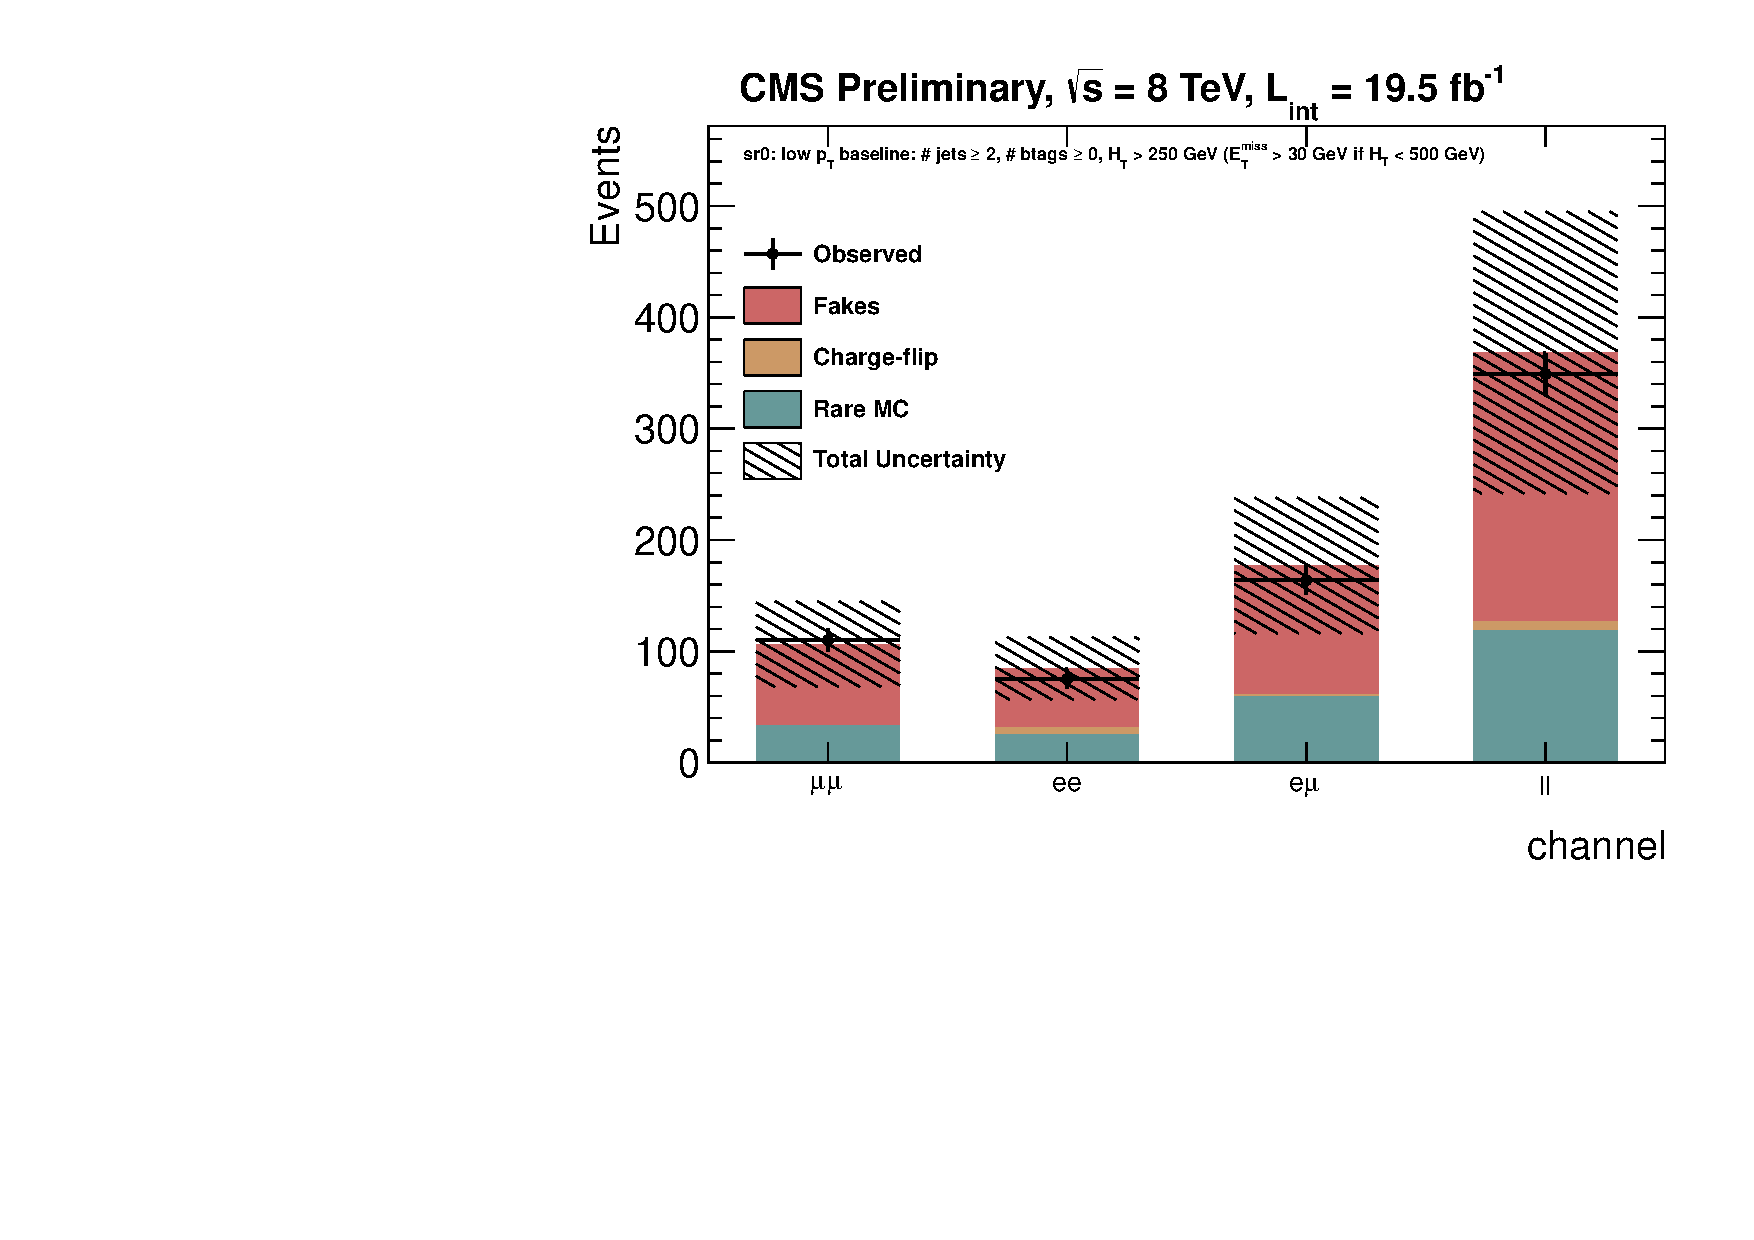
\includegraphics[width=0.49\linewidth]{p_lpt_sr0_yield}
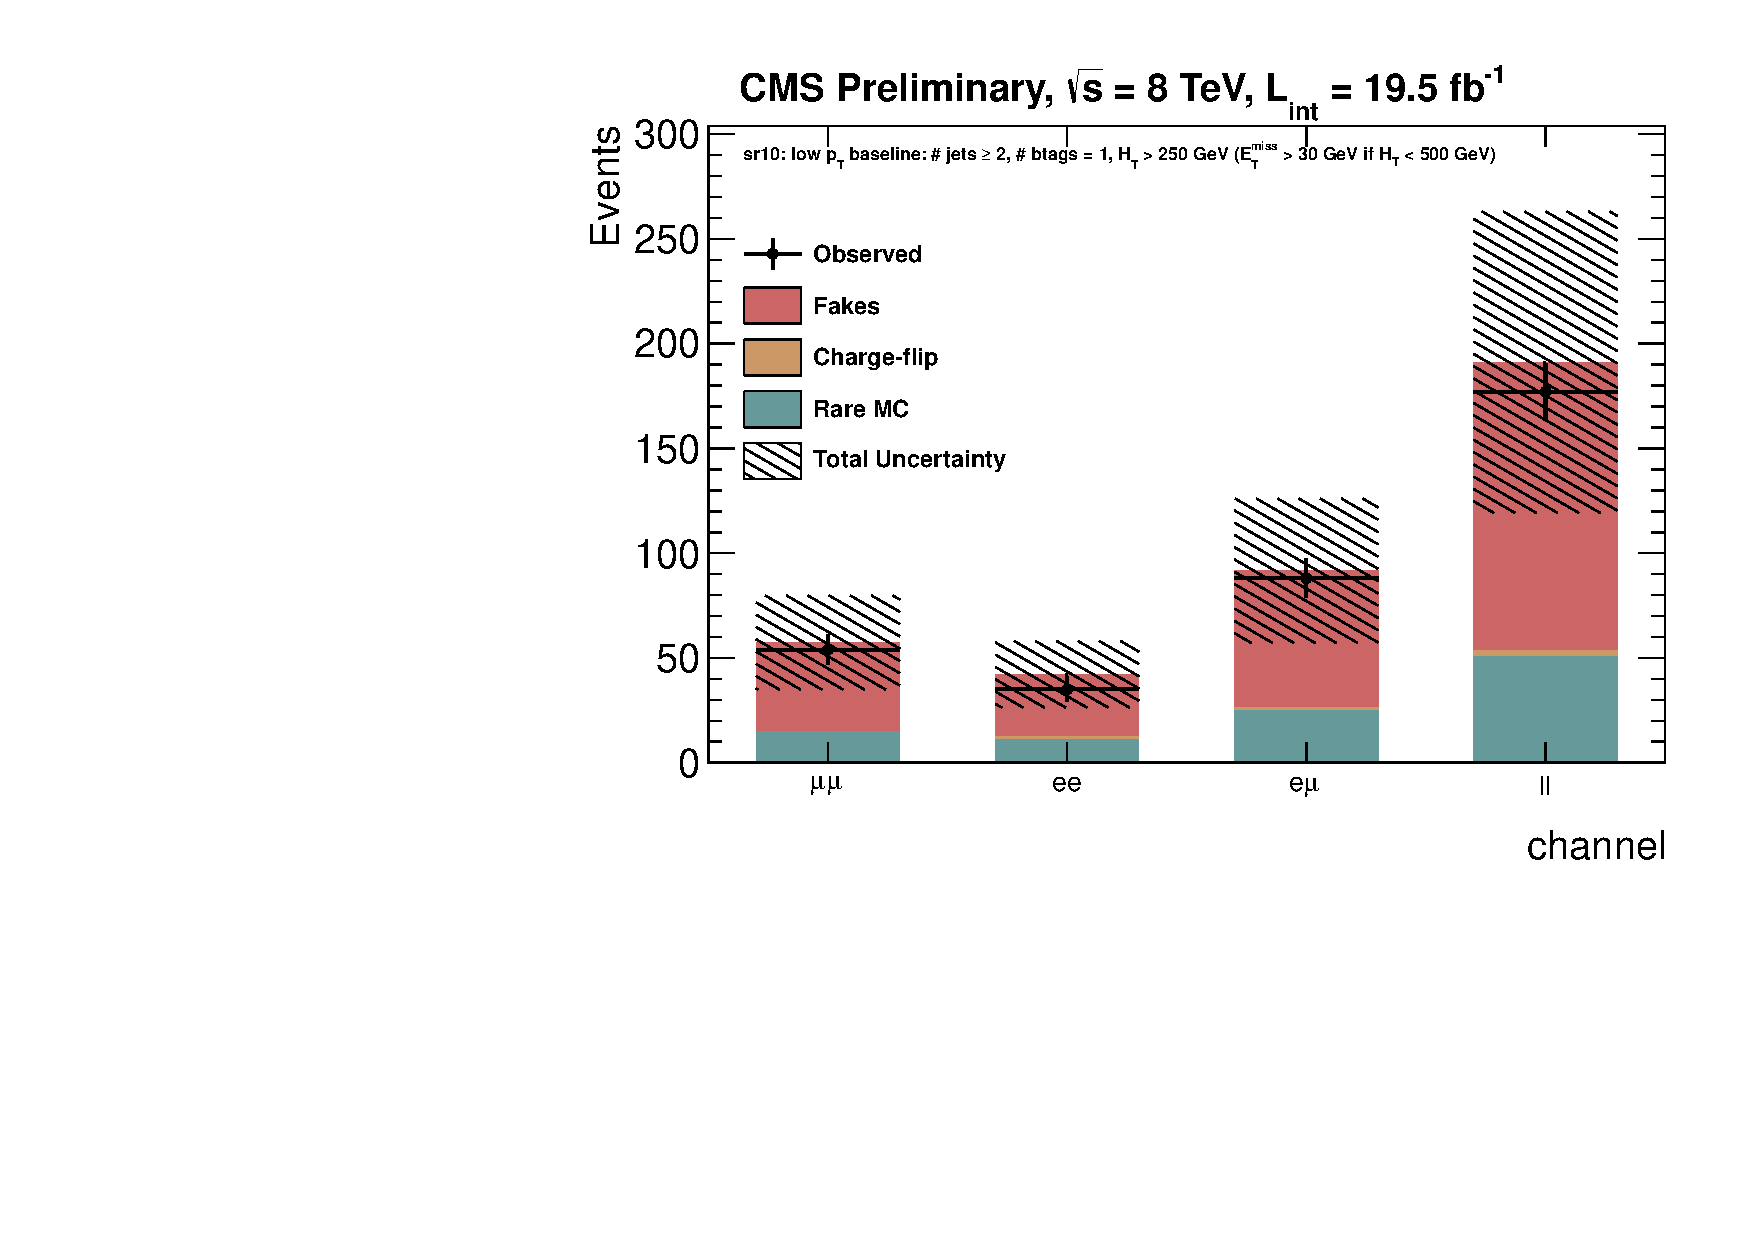
\includegraphics[width=0.49\linewidth]{p_lpt_sr10_yield}
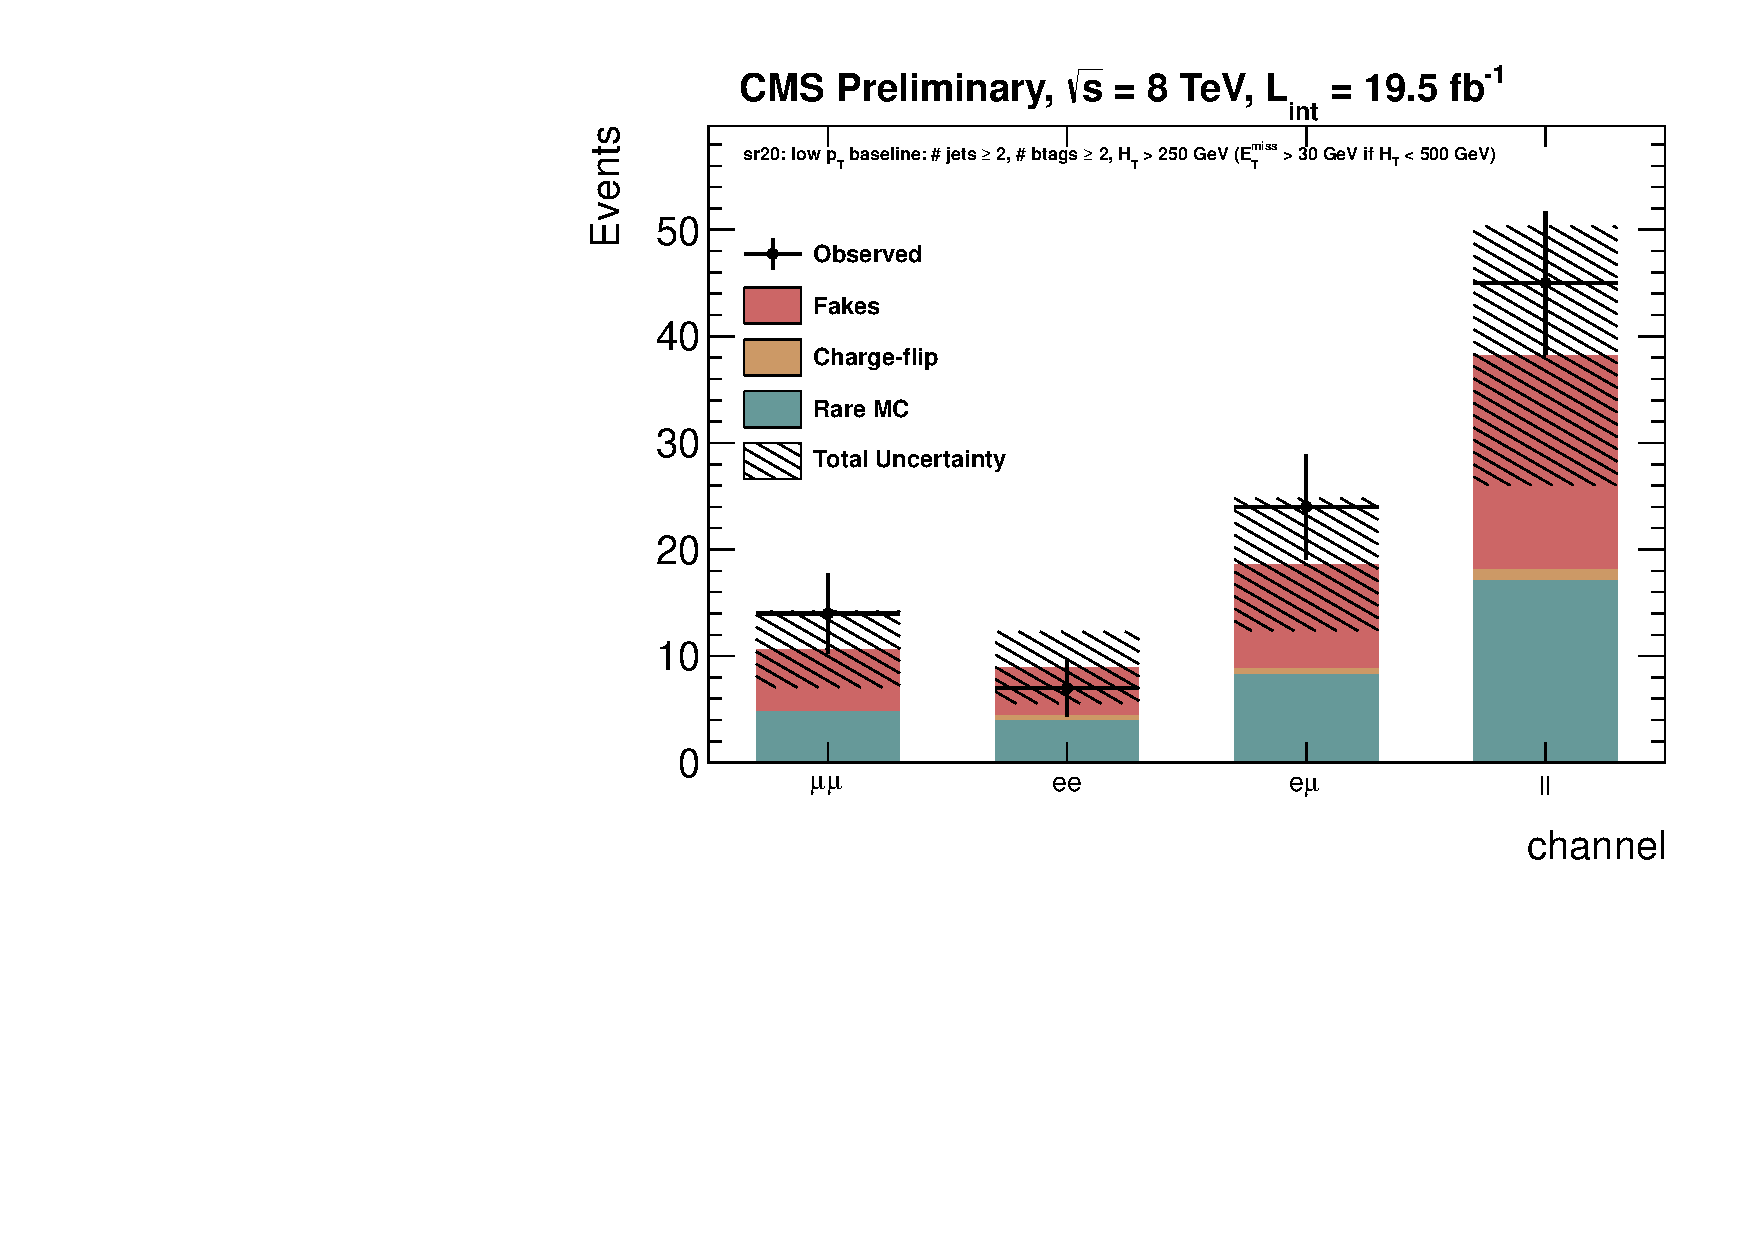
\includegraphics[width=0.49\linewidth]{p_lpt_sr20_yield}
\caption[Graphical representation of the event yields in the \lpt baseline region]
{\label{fig:results_lpt_yield_bl}
Graphical representation of the event yields in the \lpt baseline region
with no (top left), exactly one (top right) and $\geq 2$ (bottom column)
\nbtags~requirement (Search Region 0, 10 and 20). Also shown as a histogram
is the result of the background prediction. The shading around the histogram
represents the uncertainty in the background prediction.
}
\end{center}
\end{figure}

% --------------------------------------------------------------------------- %
% --------------------------------------------------------------------------- %
\subsection{Low \pt Search Regions}
\label {sec:results_lpt_sr}
% --------------------------------------------------------------------------- %

The general search regions for the \lpt analysis are defined
in Table~\ref{tab:evtsel_sr_lpt} and are repeated in
Table~\ref{tab:results_sr_lpt}. The observed yields and estimated backgrounds
for each region are shown in Table~\ref{tab:results_lpt_excl_yield_summary}.
The uncertainty is the total statistical and systematic uncertainty.
A graphical representation of these results can also be seen in
Figure~\ref{fig:results_lpt_yield_sr}. We see no evidence of an event yield in
significant excess of the background estimations.
% --------------------------------------------------------------------------- %
\begin{table}[!htb]
\begin{center}
\caption[Search regions selected for the \lpt analysis]
{\label{tab:results_sr_lpt}
Search regions selected for the \lpt search where we require
$\Ht>250\ \GeV$.
}
\begin{tabular}{c|c|c|c|c}
\hline\hline
\nbtags                   & \met                    & \njets   & \Ht[250-400] & \Ht[$>400$] \\ \hline
\multirow{4}{*}{$=0$}     & \multirow{2}{*}{50-120} & 2-3      & SR1          & SR2         \\ \cline{3-5}
                          &                         & $\geq 4$ & SR3          & SR4         \\ \cline{2-5}
                          & \multirow{2}{*}{$>120$} & 2-3      & SR5          & SR6         \\ \cline{3-5}
                          &                         & $\geq 4$ & SR7          & SR8         \\ \hline
\multirow{4}{*}{$=1$}     & \multirow{2}{*}{50-120} & 2-3      & SR11         & SR12        \\ \cline{3-5}
                          &                         & $\geq 4$ & SR13         & SR14        \\ \cline{2-5}
                          & \multirow{2}{*}{$>120$} & 2-3      & SR15         & SR16        \\ \cline{3-5}
                          &                         & $\geq 4$ & SR17         & SR18        \\ \hline
\multirow{4}{*}{$\geq 2$} & \multirow{2}{*}{50-120} & 2-3      & SR21         & SR22        \\ \cline{3-5}
                          &                         & $\geq 4$ & SR23         & SR24        \\ \cline{2-5}
                          & \multirow{2}{*}{$>120$} & 2-3      & SR25         & SR26        \\ \cline{3-5}
                          &                         & $\geq 4$ & SR27         & SR28        \\ \hline\hline
\end{tabular}
\end{center}
\end{table}  

% --------------------------------------------------------------------------- %

% --------------------------------------------------------------------------- %
\begin{table}
\begin{center}
\caption[Summary of the yields for the \lpt~analysis]
{\label{tab:results_lpt_excl_yield_summary}
A summary of the results of this search for the \lpt~analysis. For each signal
region, we show its most important kinematical requirements, the prediction for
the three background (BG) components as well as the total, and the event yield.
}
\end{center}
\resizebox{0.58\textwidth}{!}{\begin{minipage}{\textwidth}
\begin{tabular}{|c|c|c|c|c|c|c|c|c|c|}
\hline
\nbtags                   & \met                    & \njets                    & \Ht     & SR & Fake BG           & Flip BG       & Rare MC          & Total BG          & Observe \\ \hline\hline
$\geq 0$                  & 30 if $\Ht<500$ else 0  & 2                         & 250     & 0  & 241.48$\pm$121.13 & 8.43$\pm$2.58 & 118.51$\pm$59.31 & 368.42$\pm$134.89 & 349     \\ \hline       
\multirow{8}{*}{$= 0$}    & \multirow{4}{*}{50-120} & \multirow{2}{*}{2-3}      & 250-400 & 1  & 28.49$\pm$14.44   & 0.95$\pm$0.29 & 18.05$\pm$9.07   & 47.49$\pm$17.05   & 50      \\ \cline{4-5}  
                          &                         &                           & $>400$  & 2  & 5.46$\pm$2.89     & 0.41$\pm$0.13 & 7.35$\pm$3.73    & 13.22$\pm$4.72    & 17      \\ \cline{3-5}  
                          &                         & \multirow{2}{*}{$\geq 4$} & 250-400 & 3  & 10.94$\pm$5.63    & 0.12$\pm$0.04 & 2.80$\pm$1.51    & 13.86$\pm$5.83    & 13      \\ \cline{4-5}  
                          &                         &                           & $>400$  & 4  & 5.43$\pm$2.87     & 0.16$\pm$0.05 & 3.51$\pm$1.84    & 9.10$\pm$3.41     & 4       \\ \cline{2-5}  
                          & \multirow{4}{*}{$>120$} & \multirow{2}{*}{2-3}      & 250-400 & 5  & 10.48$\pm$5.41    & 0.13$\pm$0.04 & 11.78$\pm$5.93   & 22.39$\pm$8.02    & 22      \\ \cline{4-5}  
                          &                         &                           & $>400$  & 6  & 3.98$\pm$2.16     & 0.07$\pm$0.02 & 9.06$\pm$4.58    & 13.11$\pm$5.07    & 18      \\ \cline{3-5}  
                          &                         & \multirow{2}{*}{$\geq 4$} & 250-400 & 7  & 2.39$\pm$1.35     & 0.02$\pm$0.01 & 1.08$\pm$0.68    & 3.49$\pm$1.51     & 2       \\ \cline{4-5}  
                          &                         &                           & $>400$  & 8  & 4.44$\pm$2.36     & 0.03$\pm$0.01 & 3.14$\pm$1.65    & 7.60$\pm$2.88     & 4       \\ \hline       
\multirow{9}{*}{$=1$}     & 30 if $\Ht<500$ else 0  & 2                         & 250     & 10 & 117.46$\pm$58.99  & 2.00$\pm$0.61 & 33.43$\pm$16.77  & 152.88$\pm$61.33  & 132     \\ \cline{2-5}  
                          & \multirow{4}{*}{50-120} & \multirow{2}{*}{2-3}      & 250-400 & 11 & 35.51$\pm$17.93   & 0.56$\pm$0.17 & 6.29$\pm$3.20    & 42.36$\pm$18.22   & 40      \\ \cline{4-5}  
                          &                         &                           & $>400$  & 12 & 5.13$\pm$2.73     & 0.14$\pm$0.04 & 2.47$\pm$1.32    & 7.74$\pm$3.03     & 5       \\ \cline{3-5}  
                          &                         & \multirow{2}{*}{$\geq 4$} & 250-400 & 13 & 17.60$\pm$8.96    & 0.14$\pm$0.05 & 4.11$\pm$2.12    & 21.85$\pm$9.21    & 15      \\ \cline{4-5}  
                          &                         &                           & $>400$  & 14 & 9.74$\pm$5.02     & 0.10$\pm$0.03 & 3.64$\pm$1.89    & 13.47$\pm$5.36    & 6       \\ \cline{2-5}  
                          & \multirow{4}{*}{$>120$} & \multirow{2}{*}{2-3}      & 250-400 & 15 & 9.15$\pm$4.72     & 0.23$\pm$0.07 & 4.40$\pm$2.26    & 13.78$\pm$5.24    & 9       \\ \cline{4-5}  
                          &                         &                           & $>400$  & 16 & 3.16$\pm$1.73     & 0.07$\pm$0.02 & 2.75$\pm$1.46    & 5.98$\pm$2.26     & 5       \\ \cline{3-5}  
                          &                         & \multirow{2}{*}{$\geq 4$} & 250-400 & 17 & 3.58$\pm$1.94     & 0.04$\pm$0.01 & 1.61$\pm$0.92    & 5.23$\pm$2.14     & 3       \\ \cline{4-5}  
                          &                         &                           & $>400$  & 18 & 4.22$\pm$2.25     & 0.05$\pm$0.02 & 3.27$\pm$1.71    & 7.54$\pm$2.82     & 11      \\ \hline       
\multirow{9}{*}{$\geq 2$} & 30 if $\Ht<500$ else 0  & 2                         & 250     & 20 & 20.18$\pm$10.27   & 0.98$\pm$0.30 & 17.32$\pm$8.72   & 38.47$\pm$13.47   & 45      \\ \cline{2-5}  
                          & \multirow{4}{*}{50-120} & \multirow{2}{*}{2-3}      & 250-400 & 21 & 4.60$\pm$2.45     & 0.32$\pm$0.10 & 3.00$\pm$1.58    & 7.92$\pm$2.91     & 10      \\ \cline{4-5}  
                          &                         &                           & $>400$  & 22 & 0.46$\pm$0.36     & 0.06$\pm$0.02 & 0.83$\pm$0.57    & 1.35$\pm$0.68     & 1       \\ \cline{3-5}  
                          &                         & \multirow{2}{*}{$\geq 4$} & 250-400 & 23 & 4.50$\pm$2.41     & 0.11$\pm$0.03 & 2.47$\pm$1.32    & 7.07$\pm$2.75     & 6       \\ \cline{4-5}  
                          &                         &                           & $>400$  & 24 & 1.84$\pm$1.07     & 0.07$\pm$0.02 & 2.42$\pm$1.29    & 4.33$\pm$1.68     & 11      \\ \cline{2-5}  
                          & \multirow{4}{*}{$>120$} & \multirow{2}{*}{2-3}      & 250-400 & 25 & 1.05$\pm$0.65     & 0.10$\pm$0.03 & 1.57$\pm$0.89    & 2.72$\pm$1.11     & 1       \\ \cline{4-5}  
                          &                         &                           & $>400$  & 26 & 0.34$\pm$0.29     & 0.03$\pm$0.01 & 0.89$\pm$0.59    & 1.25$\pm$0.66     & 2       \\ \cline{3-5}  
                          &                         & \multirow{2}{*}{$\geq 4$} & 250-400 & 27 & 0.95$\pm$0.60     & 0.03$\pm$0.01 & 0.83$\pm$0.58    & 1.81$\pm$0.83     & 0       \\ \cline{4-5}  
                          &                         &                           & $>400$  & 28 & 1.29$\pm$0.79     & 0.04$\pm$0.01 & 2.07$\pm$1.12    & 3.40$\pm$1.37     & 3       \\ \hline       
\end{tabular}
\end{minipage}
}
\end{table}
% --------------------------------------------------------------------------- %
\begin{figure}[!hbt]
\begin{center}
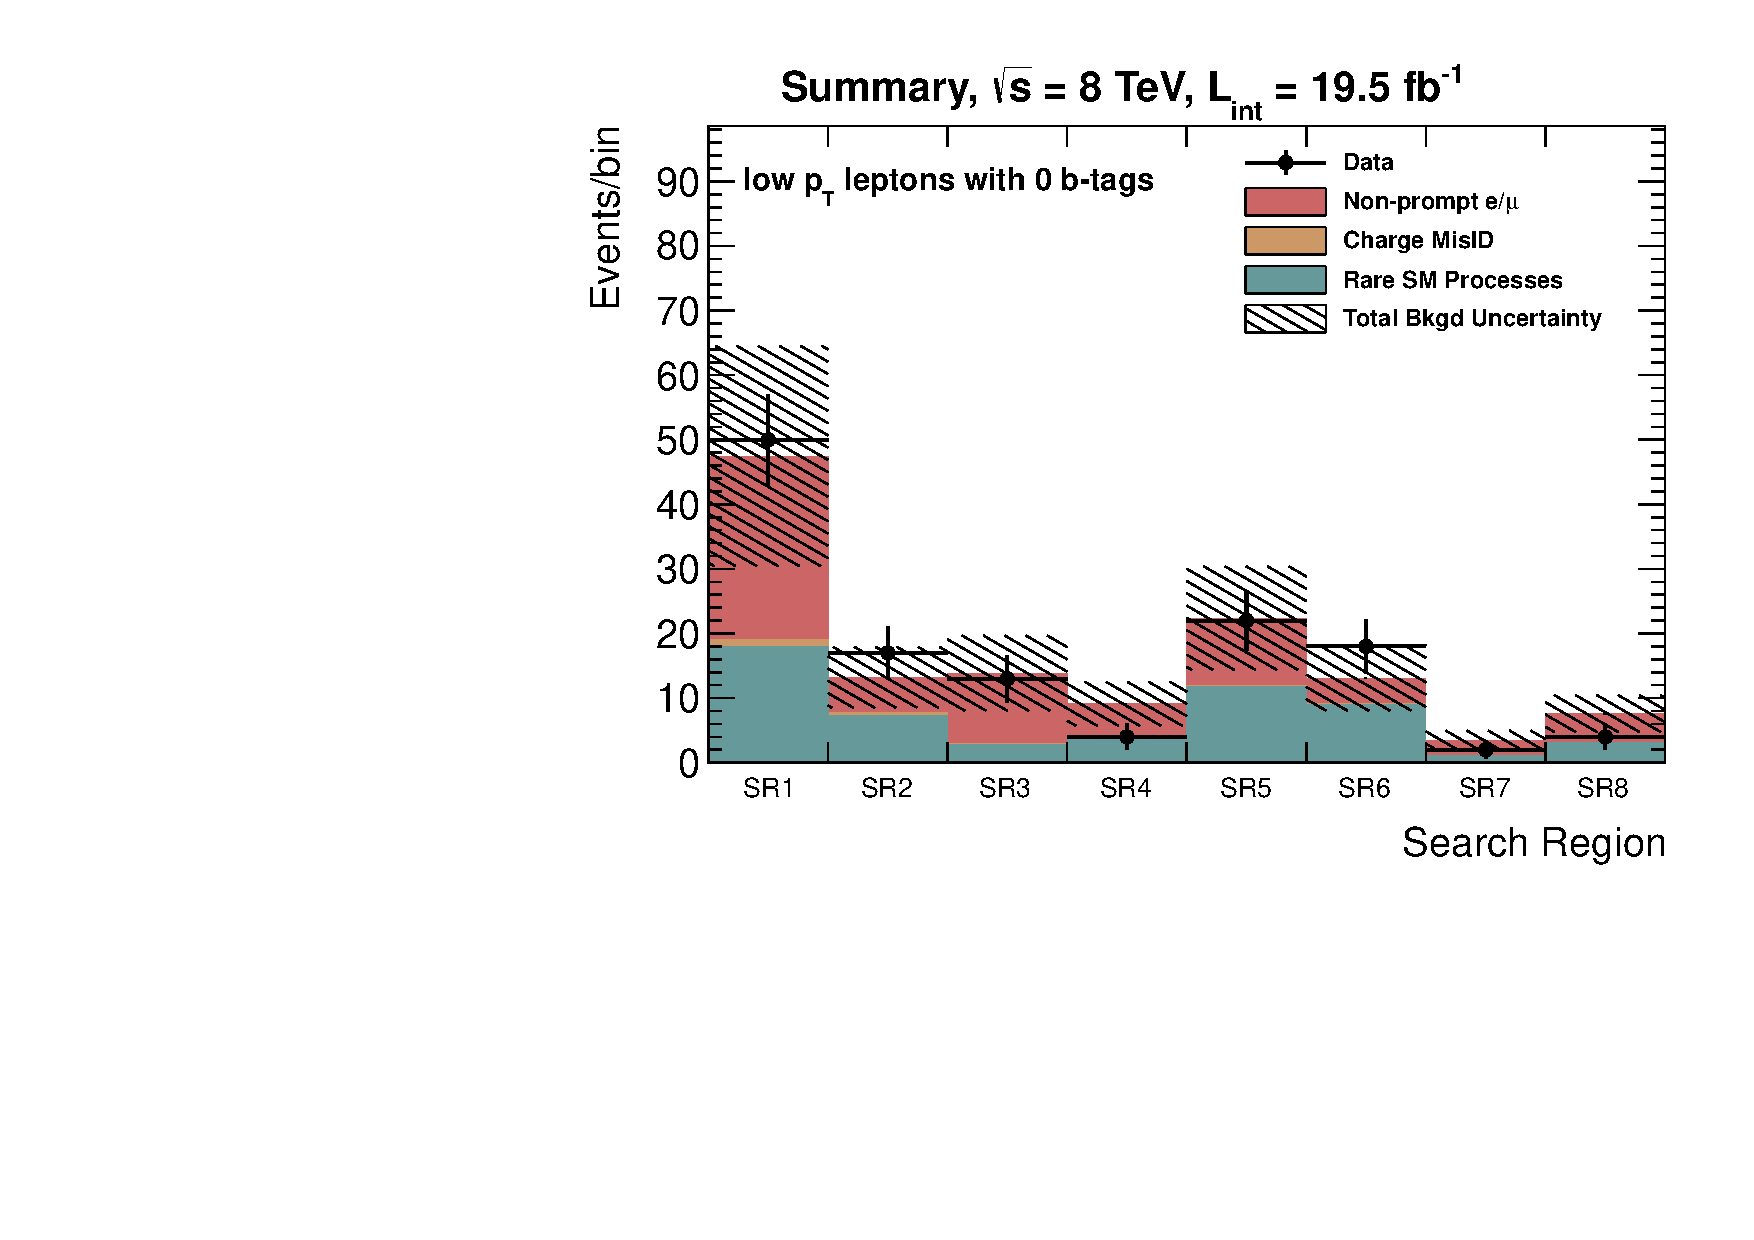
\includegraphics[width=0.49\linewidth]{p_yields_lpt_exclusive_nb0}
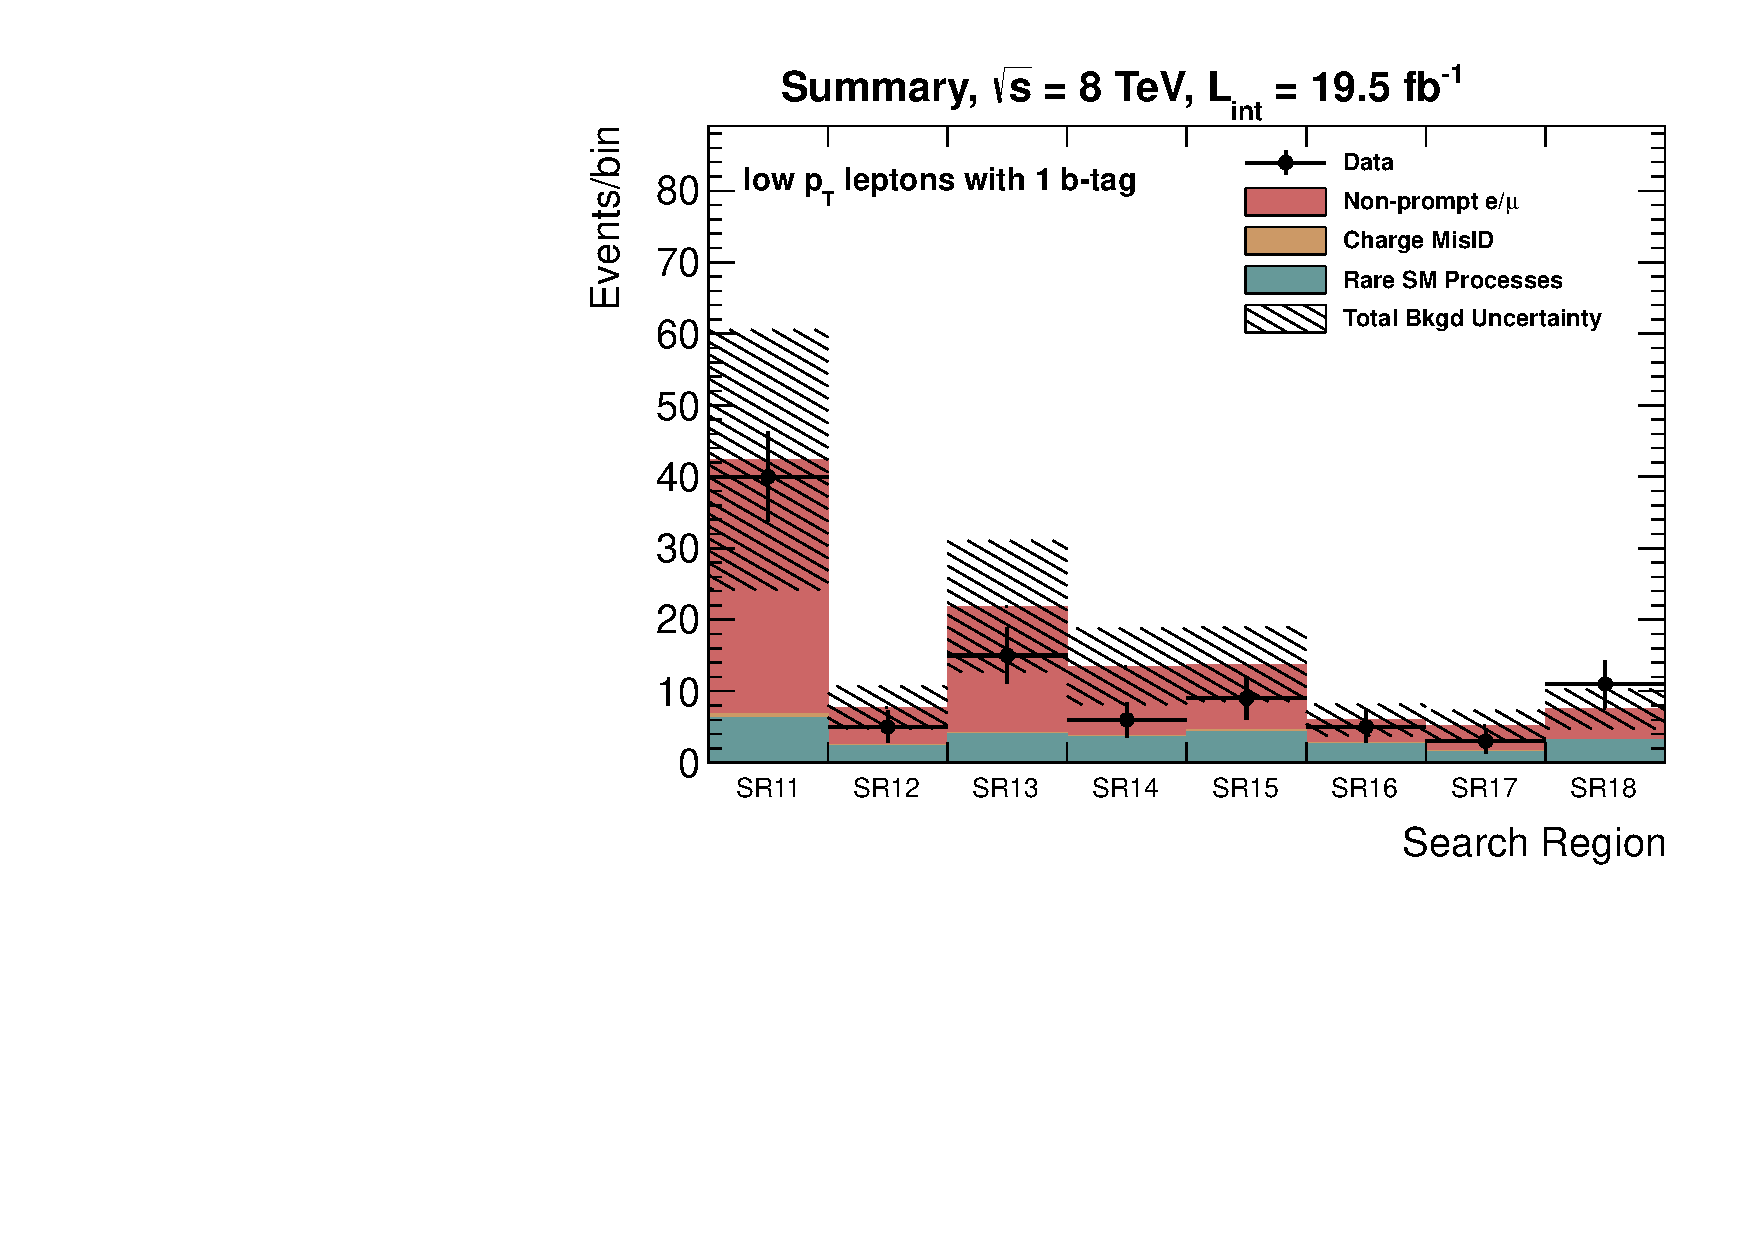
\includegraphics[width=0.49\linewidth]{p_yields_lpt_exclusive_nb1}
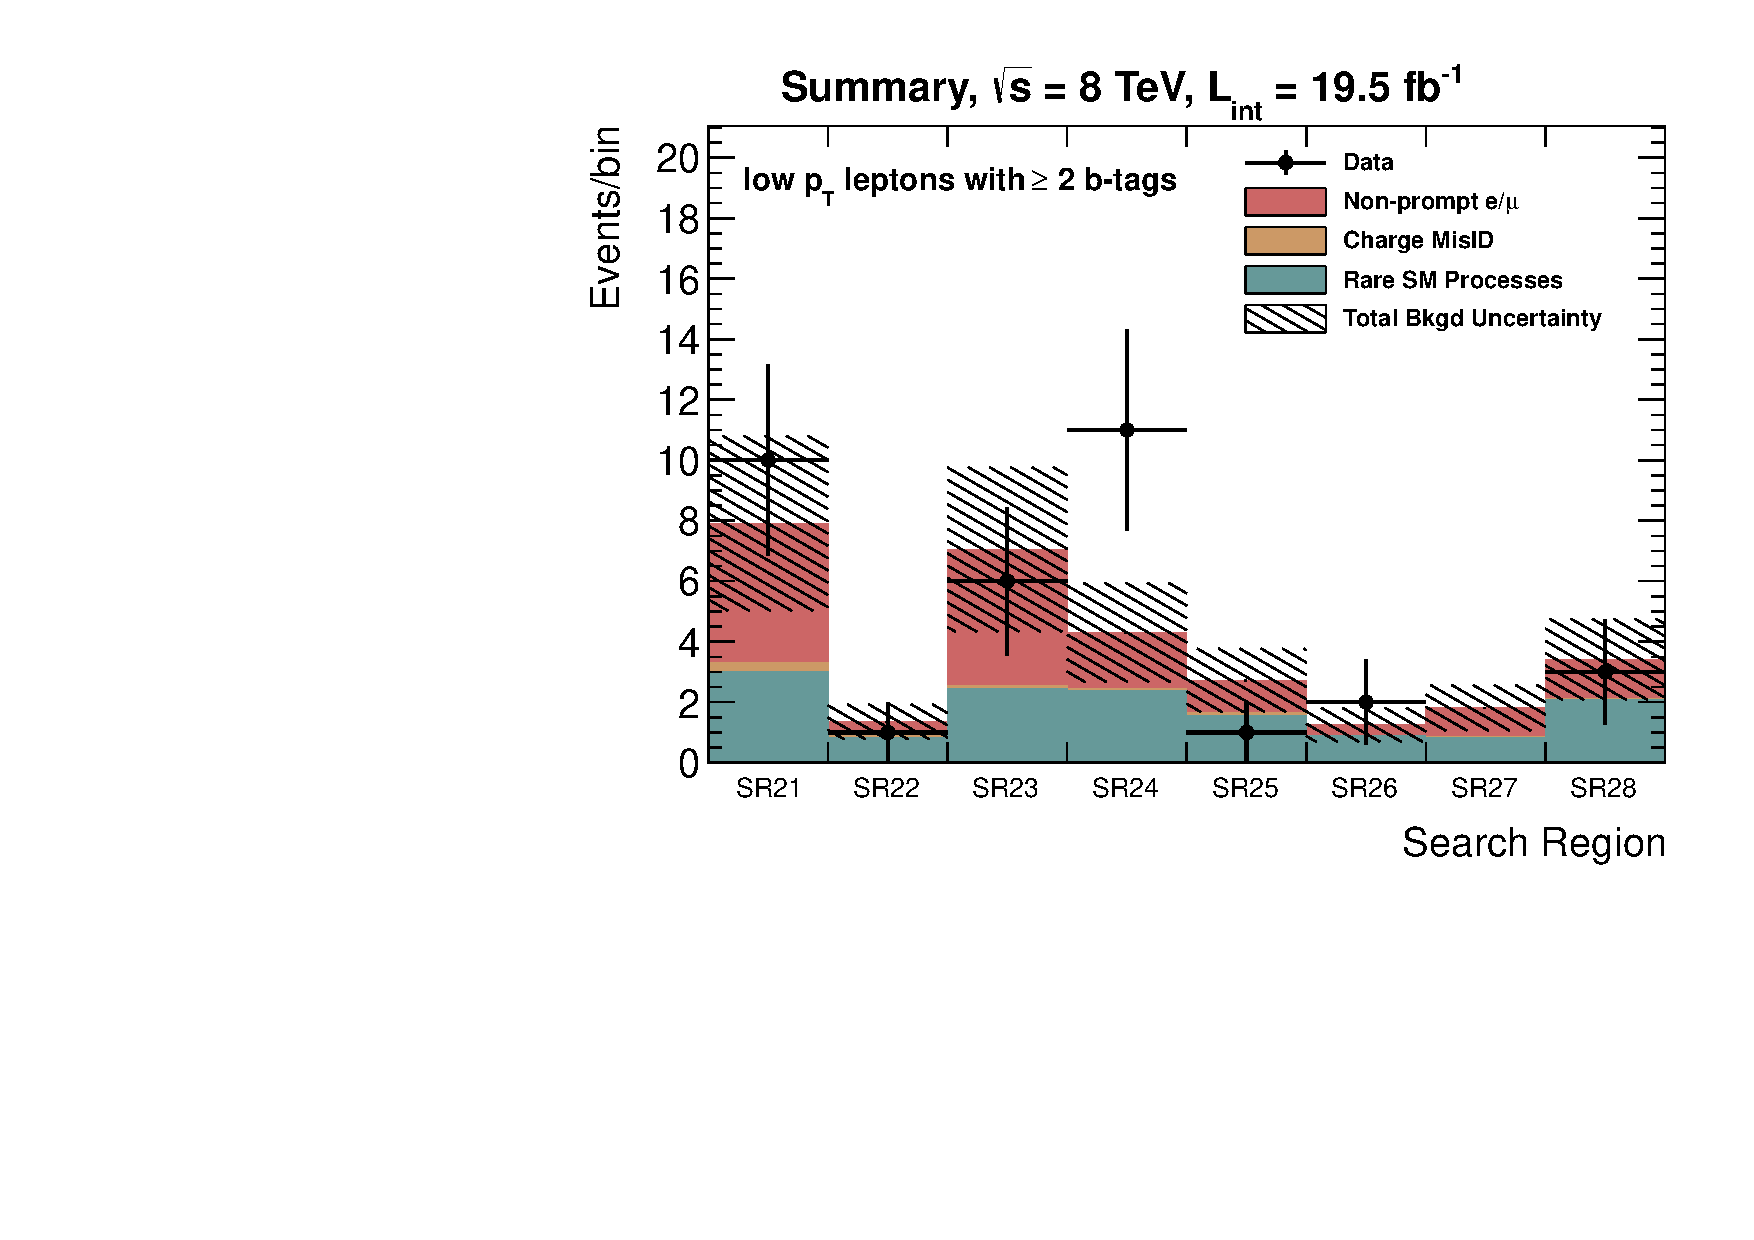
\includegraphics[width=0.49\linewidth]{p_yields_lpt_exclusive_nb2}
\caption[Graphical representation of the event yields in the \lpt search regions]
{\label{fig:results_lpt_yield_sr}
Graphical representation of the event yields in the \lpt search regions
with one (top left), exactly one (top right) and $\geq 2$ (bottom column)
\nbtags~requirement (Search Region 1-8, 11-18, and 21-28). Also shown as a histogram
is the result of the background prediction. The shading around the histogram
represents the uncertainty in the background prediction.
}
\end{center}
\end{figure}
% --------------------------------------------------------------------------- %
In the various search regions, irreducible backgrounds, primarily from \ttW,
\WZ and \qqWW, are the dominant backgrounds at approximately 15-70\%, depending
on the search region. Fake leptons account for approximately 25-80\% of the
background also depending on the search region. The background from charge
mis-reconstruction is small contributing less than 5\%.
\clearpage

% --------------------------------------------------------------------------- %
% --------------------------------------------------------------------------- %
\section{Interpretations}
\label {sec:results_int}
% --------------------------------------------------------------------------- %
% --------------------------------------------------------------------------- %
Given the lack of a significant excess over the expected SM background, the
results of the search are used to place limits on the cross section of rare SM
processes and on the parameters of various models of new physics. In total,
we have 54 search regions (SR) for this analysis, but for the limit setting
procedure for each model we take into account only the dedicated search regions
as described in Section~\ref{sec:evtsel_sr}. For each model in consideration,
all relevant search regions are included into a multi-bin fit in order to
maximize sensitivity. The 95\% confidence level (CL) upper limits on the signal
yields are calculated using the modified frequentist CL$_s$ method. Formally we
construct a likelihood function, i.e.,
%==========================================================================================
\begin{eqnarray}\label{eq:likelihood}
\lumi ({\rm data}|\mu,\theta) = {\rm Poisson } \Bigl({\rm data}|\mu \cdot s(\theta) + b(\theta)\Bigr) \cdot p\left(\hat{\theta}|\theta\right),
\end{eqnarray}
%==========================================================================================
where ``data'' represents our observed yields, and Poisson(data$|$
$\mu$,$\theta$) represents the product of probabilities to observe $n_i$ events
in the $i$th region, i.e.,
%==========================================================================================
\begin{eqnarray}
\prod_i \frac{ \left(\mu s_i + b_i\right)^{n_i}}{n_i!} e^{-\mu s_i-b_i}.
\end{eqnarray}
%==========================================================================================
Here, the parameter $\mu$ represents our signal strength modifier and
corresponds to $\sigma \times BR$ in the context of the R-parity-conserving
simplified SUSY models (SMS)~\cite{sms}. The parameter $\theta$ denotes the
collection of nuisance parameters that can influence the values of $b$ and
$s$. Log-normal pdf's are assumed for the signal and background nuisance
parameters. These are taken to be either 0\% or 100\% correlated where
appropriate. The profile likelihood ratio is used to test the compatibility
of the observed data with the background-only and signal+background
hypotheses. The full prescription of the statistical model can be found
elsewhere~\cite{Read:2002hq,ATL-PHYS-PUB-2011-011,Junk:1999kv}.

In this section, we first give the upper limits on the cross sections for
same-sign top production followed by the Standard Model four top production.
We conclude this chapter with the limits on various Supersymmetry models
with Simplified Model Spaces (SMS), which can lead to a same-sign dilepton
signature.

% --------------------------------------------------------------------------- %
\subsection{Same-Sign Top}
\label {sec:results_int_sstop}
% --------------------------------------------------------------------------- %
The results of the search regions SStop1, SStop1++, SStop2, and SStop2++
are used to set limits on the cross section for same-sign top-quark pair
production, $\sigma(\Pp \Pp \to \cPqt \cPqt + \cPaqt \cPaqt)$ from SStop1 and
SStop2, and $\sigma(\Pp \Pp \to \cPqt \cPqt)$ from SStop1++ and SStop2++.
Here $\sigma(\Pp \Pp \to \cPqt \cPqt + \cPaqt \cPaqt)$ is short hand for the
sum $\sigma(\Pp \Pp \to \cPqt \cPqt)+\sigma(\Pp \Pp \to \cPaqt \cPaqt)$. Note
that in most new physics scenarios $\Pp \Pp \to \cPaqt \cPaqt$ is suppressed
with respect to $\Pp \Pp \to \cPqt \cPqt$ because of the parton distribution
functions of the proton. These limits are calculated using an acceptance
obtained using simulated $\Pp \Pp \to \cPqt \cPaqt$ events and an opposite-sign
selection. This acceptance, including branching fractions, is $0.43\%$
($0.26\%$) for SStop1 (SStop2) search region. The relative uncertainty on
this acceptance is $14\%$. The observed upper limits are $\sigma(\Pp \Pp \to
\cPqt \cPqt + \cPaqt \cPaqt) < 0.71$ pb and $\sigma(\Pp \Pp \to \cPqt \cPqt)
< 0.33\unit{pb}$ at 95\% CL; the median expected limits are 0.48 and 0.30
\unit{pb}, respectively.  The full procedure was documented in~\cite{an_ssb2012}.
% --------------------------------------------------------------------------- %
\subsection{Standard Model Four Top}
\label {sec:results_int_tttt}
% --------------------------------------------------------------------------- %
Similarly, the results from search regions SR21--SR28 and high-\pt lepton
selection are used to set limits on the SM cross section for the Standard
Model four-top-quark production. The observed upper limit is $\sigma(\Pp \Pp
\to \cPqt \cPqt \cPaqt \cPaqt) < 47$\unit{fb} at 95\% CL, compared to a
median expected limit of 36\unit{fb}. The SM cross section as computed
with the MC$@$NLO program~\cite{Frixione:2002ik} is $\sigma_{\rm SM} =
\left(9.14\pm0.05\right) \times10^{-1}~{\rm fb}$. The most sensitive search
regions, SR24 and SR28, have a signal acceptance of 0.52\% and 0.49\%,
respectively, with relative uncertainties of 13\% and 17\%.

% --------------------------------------------------------------------------- %
\subsection{Supersymmetry}
\label {sec:results_int_susy}
% --------------------------------------------------------------------------- %

Next, we present limits on the parameter spaces of various
R-parity-conserving simplified Supersymmetry models (SMS)~\cite{sms}.
The exclusion contours are obtained with the gluino (sbottom)
pair production cross-sections at the NLO + NLL accuracy that
are calculated in the limit where other sparticles are heavy and
decoupled~\cite{bib-nlo-nll-01,bib-nlo-nll-02,bib-nlo-nll-03,bib-nlo-nll-04,
bib-nlo-nll-05,Kramer:2012bx}. The production of SUSY particles and
the decay chains under consideration are shown schematically in
Figure~\ref{fig:results_feyn_models} and the summary of the search regions used
for each SMS model is given in Table~\ref{tab:results_models_srs} with the
results from each model discussed below.
% --------------------------------------------------------------------------- %
\begin{figure}[!htb]
\begin{center}
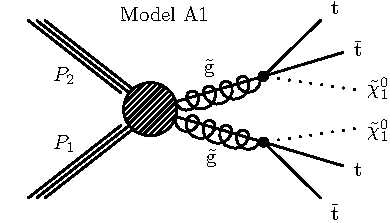
\includegraphics[width=0.45\linewidth]{T1tttt} \hfill
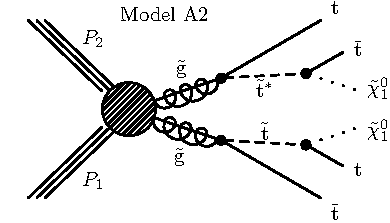
\includegraphics[width=0.45\linewidth]{T5tttt}
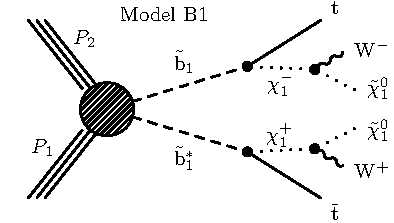
\includegraphics[width=0.45\linewidth]{T6ttWW} \hfill
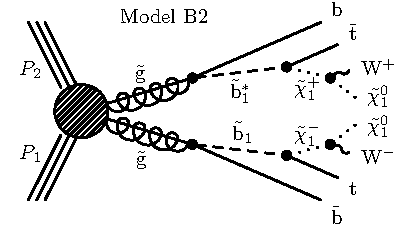
\includegraphics[width=0.45\linewidth]{T7btW}
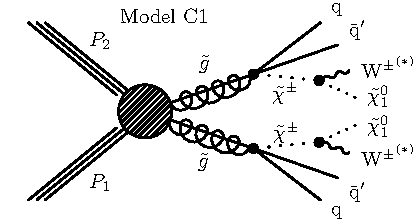
\includegraphics[width=0.45\linewidth]{T5WW} \hfill
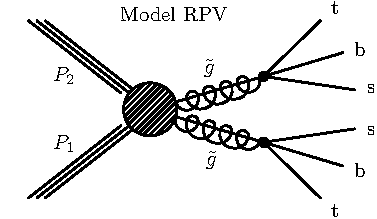
\includegraphics[width=0.45\linewidth]{T1tbs}
\caption[Diagrams for the four SUSY models considered]
{\label{fig:results_feyn_models}
Feynman diagrams for the four SUSY models considered (A1, A2, B1, B2, C1 and RPV).
}
\end{center}
\end{figure}
% --------------------------------------------------------------------------- %
\begin{table}[!hbt]
\begin{center}
\caption[Summary of the search regions used for limit setting in each SMS model considered]
{\label{tab:results_models_srs}
Summary of the search regions used for limit setting in each SMS model considered.
}
\begin{tabular}{|c|c|c|c|}
\hline\hline
Model                                     & Model Restriction                                & Analysis Type & Signal Regions Used \\ \hline\hline
A1                                        &                                                  & high-$\pt$    & 21--28              \\ 
A2                                        & m$_{\chiz}$ = 50 GeV                             & high-$\pt$    & 21--28              \\ 
B1                                        & m$_{\chiz}$ = 50 GeV                             & high-$\pt$    & 11--18, 21--28      \\ 
B1                                        & x = $\text{m}_{\chiz}/\text{m}_{\chipm_1} = 0.5$ & high-$\pt$    & 11--18, 21--28      \\ 
B1                                        & x = $\text{m}_{\chiz}/\text{m}_{\chipm_1} = 0.8$ & low-$\pt$     & 11--18, 21--28      \\ 
B2                                        & m$_{\chiz}$ = 50 GeV, m$_{\chipm_1}$ = 150 GeV   & high-$\pt$    & 21--28              \\ 
B2                                        & m$_{\chiz}$ = 50 GeV, m$_{\chipm_1}$ = 300 GeV   & high-$\pt$    & 21--28              \\ 
C1                                        & x = 0.5                                          & high-$\pt$    & 01--08              \\ 
C1                                        & x = 0.8                                          & low-$\pt$     & 01--08              \\ 
RPV                                       &                                                  & high-$\pt$    & RPV2                \\ 
% $pp \to tt + \overline{t}\overline{t}$    &                                                  & high-$\pt$ & SStop1, SStop2      \\ 
% $pp \to tt$                               &                                                  & high-$\pt$ & SStop1++, SStop2++  \\ 
% $pp \to tt\overline{t}\overline{t}$       &                                                  & high-$\pt$ & 21--28              \\ 
\hline\hline
\end{tabular}
\end{center}
\end{table}
% --------------------------------------------------------------------------- %
\clearpage
Scenarios A1 and A2 represent models of gluino pair production resulting in the
$\cPqt \cPqt \cPaqt \cPaqt \chiz_1 \chiz_1$ final state, where $\chiz_1$ is the
lightest neutralino~\cite{stopVirtual,stopVirtualPRD,sms,wacker,naturalness4}.
In model A1, the gluino undergoes a three-body decay $\sGlu \to \ttbar \chiz_1$
mediated by an off-shell top squark. In model A2, the gluino decays to a top
quark and an anti-top squark, with the on-shell anti-squark further decaying
into an anti-top quark and a neutralino. Both of these models produce four
on-shell W bosons and four bottom quarks. Therefore, these models can be probed with
search regions SR21--SR28 where at least two b-tagged jets and \hpt leptons
are required, the region with the best sensitivity is SR28. The 95\% CL upper
limits on the cross section times branching ratio, as well as the exclusion
contours, are shown in Figure~\ref{fig:results_limit_a12}. For model A1 these
are presented as a function of gluino mass and $\chiz_1$ mass and for model
A2 as a function of gluino mass and stop mass for $\chiz_1$ mass set to 50
\GeV.
% --------------------------------------------------------------------------- %
\begin{figure}[!tbh]
\begin{center}
\includegraphics[width=0.49\linewidth]{p_limit_T1tttt}
\includegraphics[width=0.49\linewidth]{p_limit_T5tttt}
\caption[Exclusion curves for models A1 and A2]
{\label{fig:results_limit_a12}
Exclusion regions at 95\% CL in the planes of $m(\chiz_1)$ \vs $m(\sGlu)$
(model A1) and $m(\sTop_1)$ \vs $m(\sGlu)$ (model A2). The excluded
regions are those within the kinematic boundaries and to the left
of the curves. The effects of the theoretical uncertainties in the
next-to-leading-order plus next-to-leading-log calculations of the production
cross sections~\cite{kramer_2012bx} are indicated by the black-thin curves; the
expected limits and their $\pm$1 standard-deviation variations are also shown
in dashed red curves.
}
\end{center}
\end{figure}
% --------------------------------------------------------------------------- %
\clearpage

Model B1 is a model of bottom-squark pair production, followed by one of the
most likely decay modes of the bottom squark, $\sBot_1 \to \cPqt \chim_1$
and $\chim_1 \to \PWm \chiz_1$. We consider three scenarios in this decay
mode. We either fix the $\chiz_1$ mass at 50~\GeV and present the limits in
the $m_{\sBot_1}$--$m_{\chipm_1}$ plane, or use $m_{\sBot_1}$--$m_{\chiz_1}$
plane with variable mass of $m_{\chipm_1}$ using the equation $m_{\chipm_1} 
=  xm_{\chiz_1}  +  (1-x)m_{\sBot_1}$ with $x=0.5$ or $x=0.8$. The value of
$x$ determines whether the top and W are produced on- or off-shell. The limits
on this model, obtained using search regions SR11 to SR28, are presented in
Figure~\ref{fig:results_limit_b12}. For the $x=0.8$ scenario the low-\pt lepton selection
is used, while high-\pt leptons are used for the other two scenarios. SR28 is
again the most sensitive search region, followed by the regions requiring one
b-tagged jet: SR18, SR15, and SR13.

Model B2 consists of gluino pair production followed by $\sGlu \to \sBot_1
\cPaqb$. The gluino decay modes in models A1 and A2 would be dominant if the
top squark is the lightest supersymmetric quark. Conversely, if the bottom
squark is the lightest, the decay mode in model B2 would be the most probable.
The limits on this model, calculated using search regions SR21--SR28 and the
high-\pt lepton selection, are presented as a function of $m(\sBot_1)$ and
$m(\sGlu)$ for two fixed masses of $m_{\chipm_1}$, 150 and 300 \GeV. The region
with the largest sensitivity to this model is SR28.
% --------------------------------------------------------------------------- %
\begin{figure}[!tbh]
\resizebox{0.93\textwidth}{!}{\begin{minipage}{\textwidth}
\begin{center}
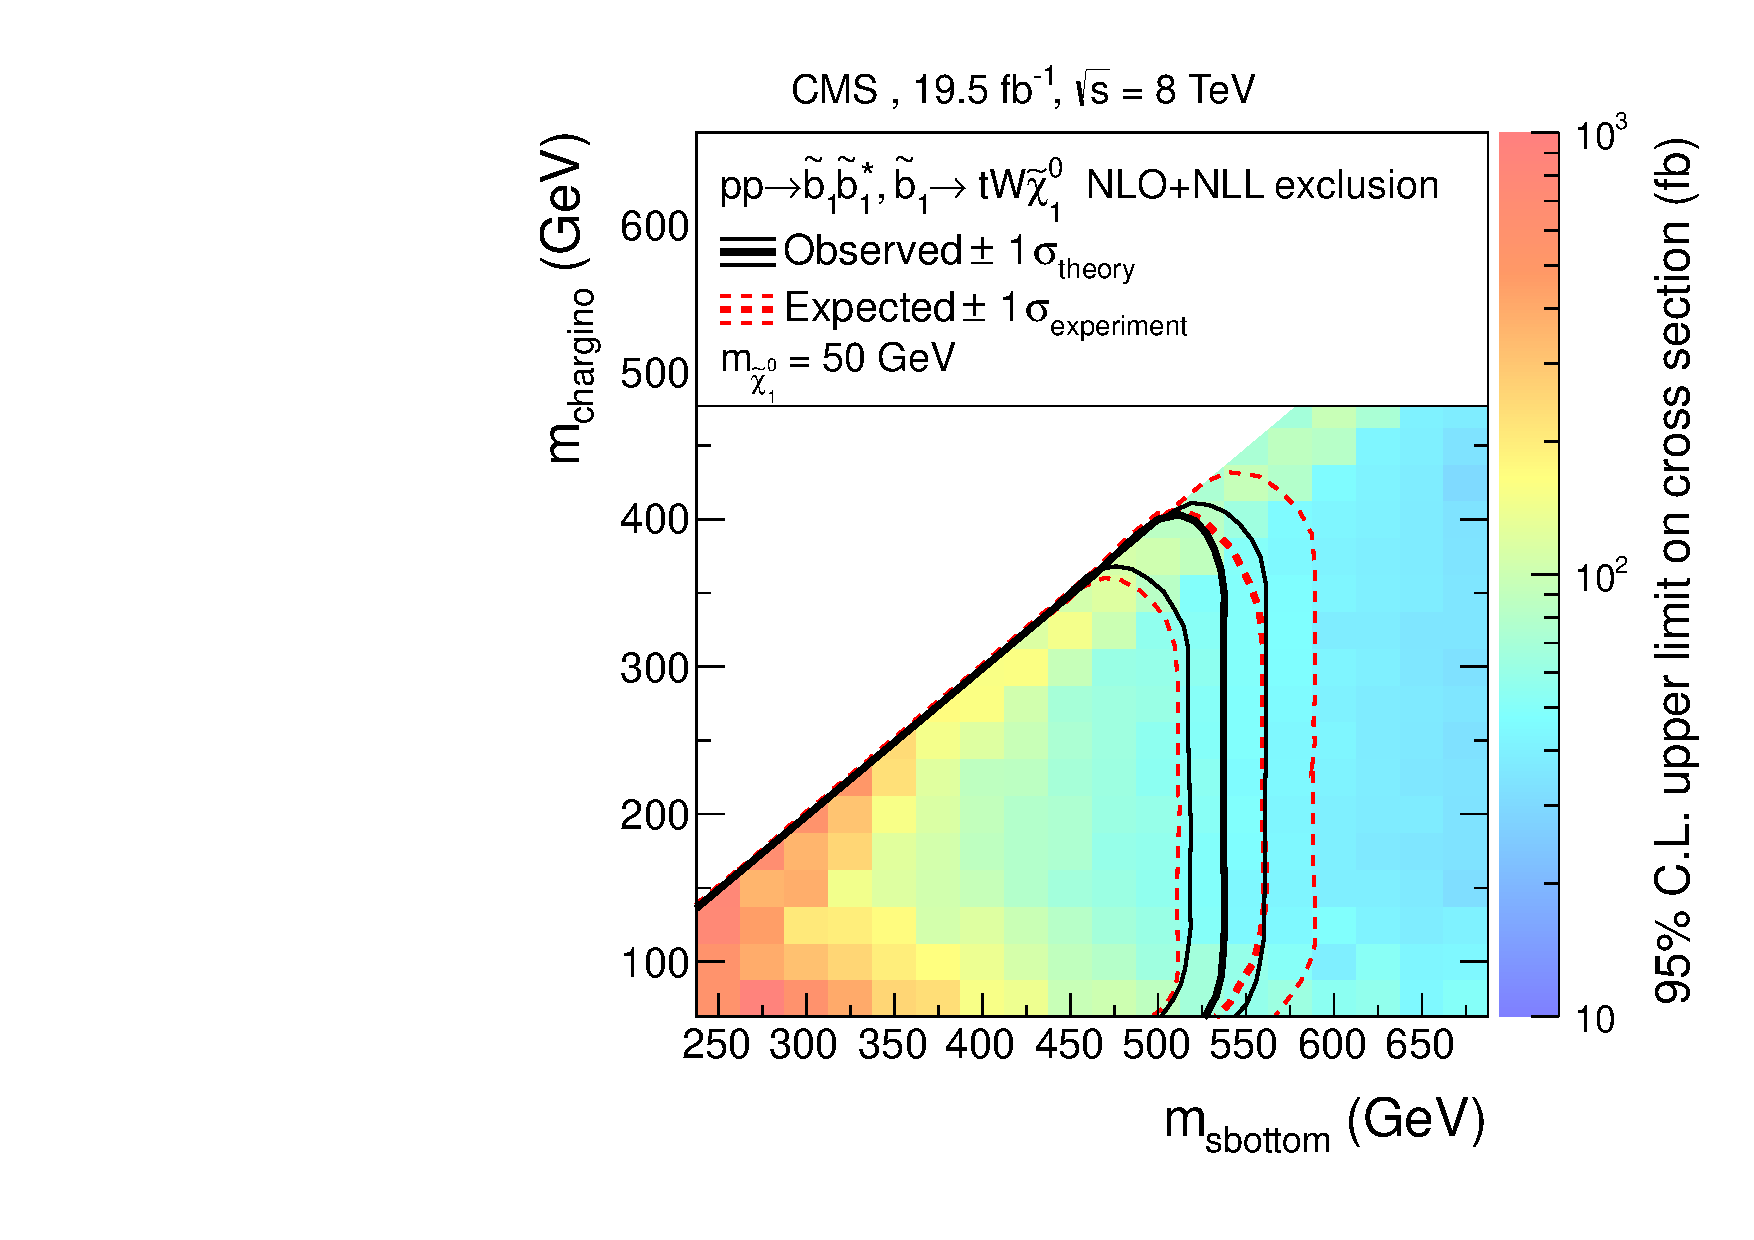
\includegraphics[width=0.49\linewidth]{p_limit_t6ttww} \\
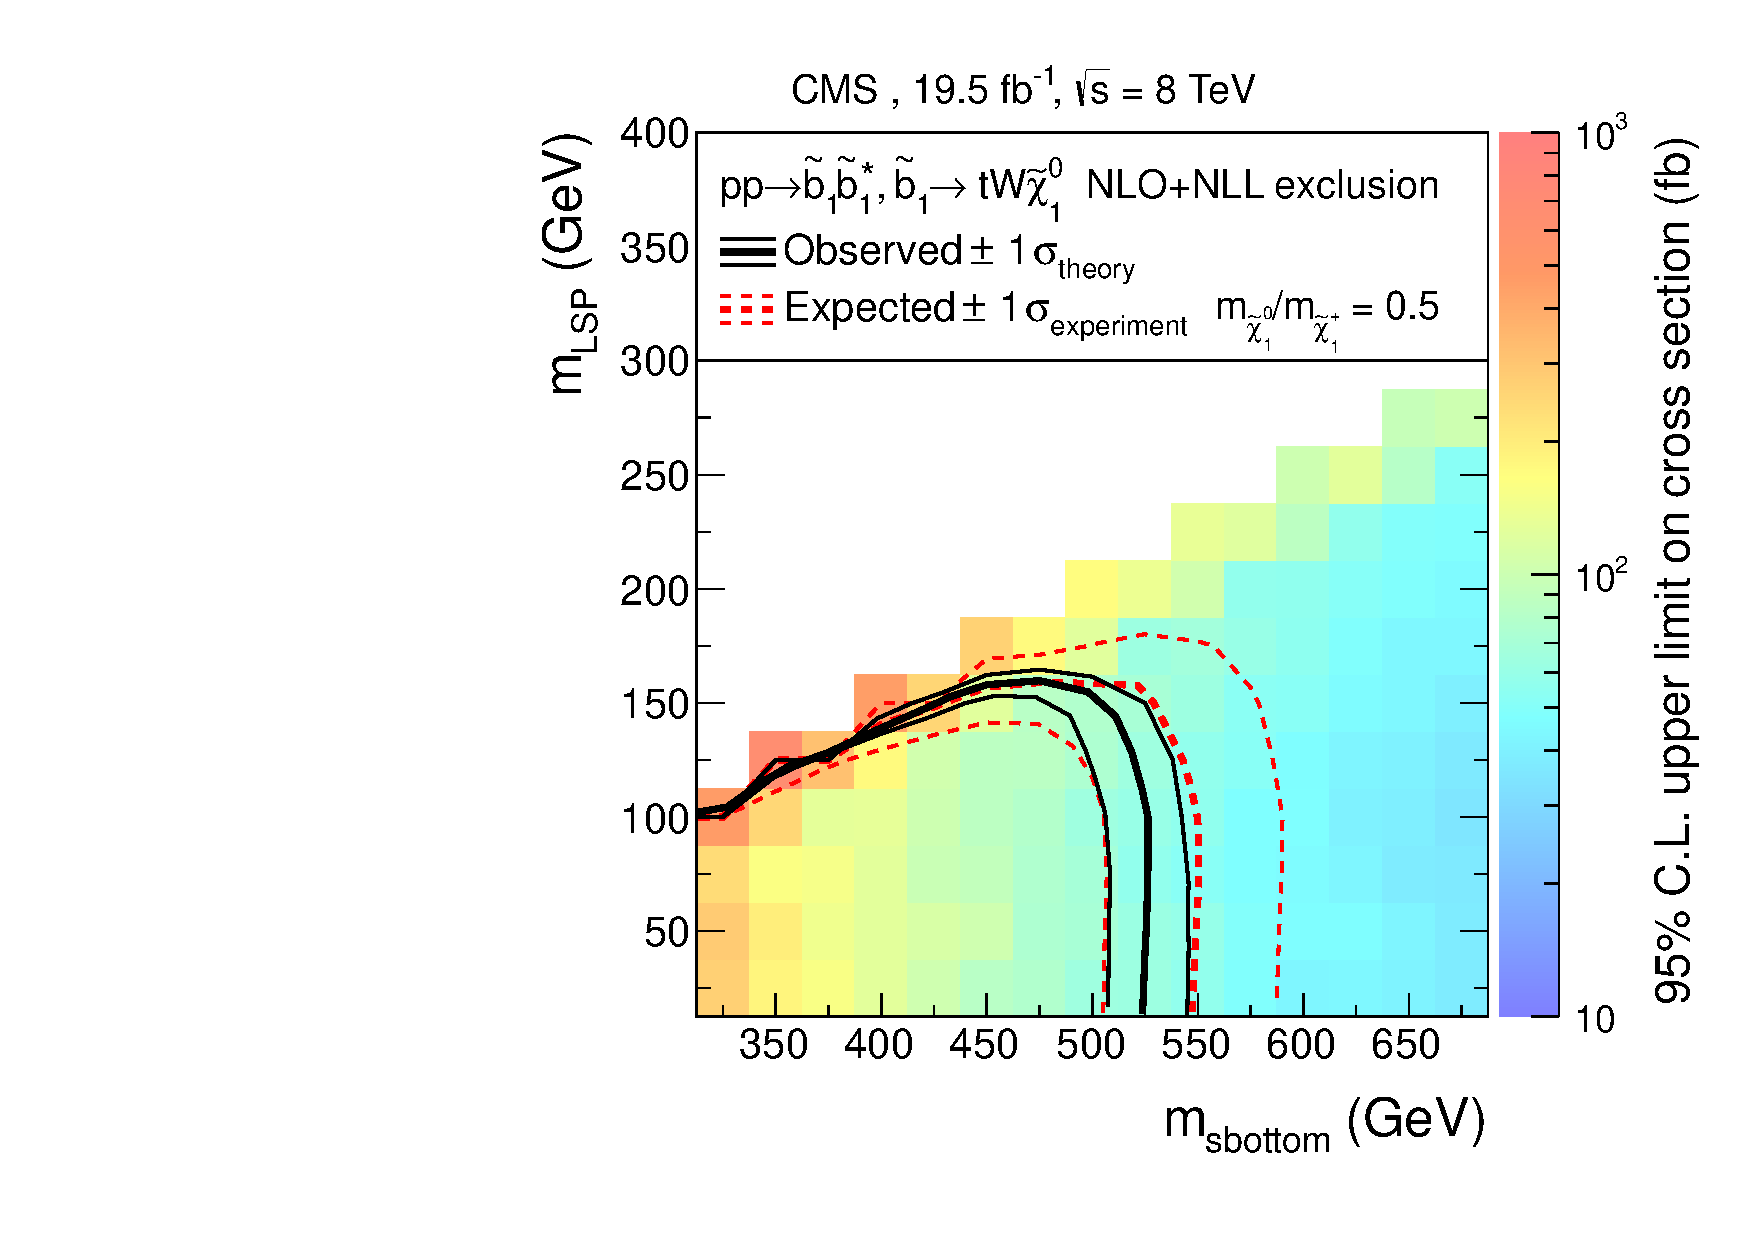
\includegraphics[width=0.49\linewidth]{p_limit_t6ttww_x05}
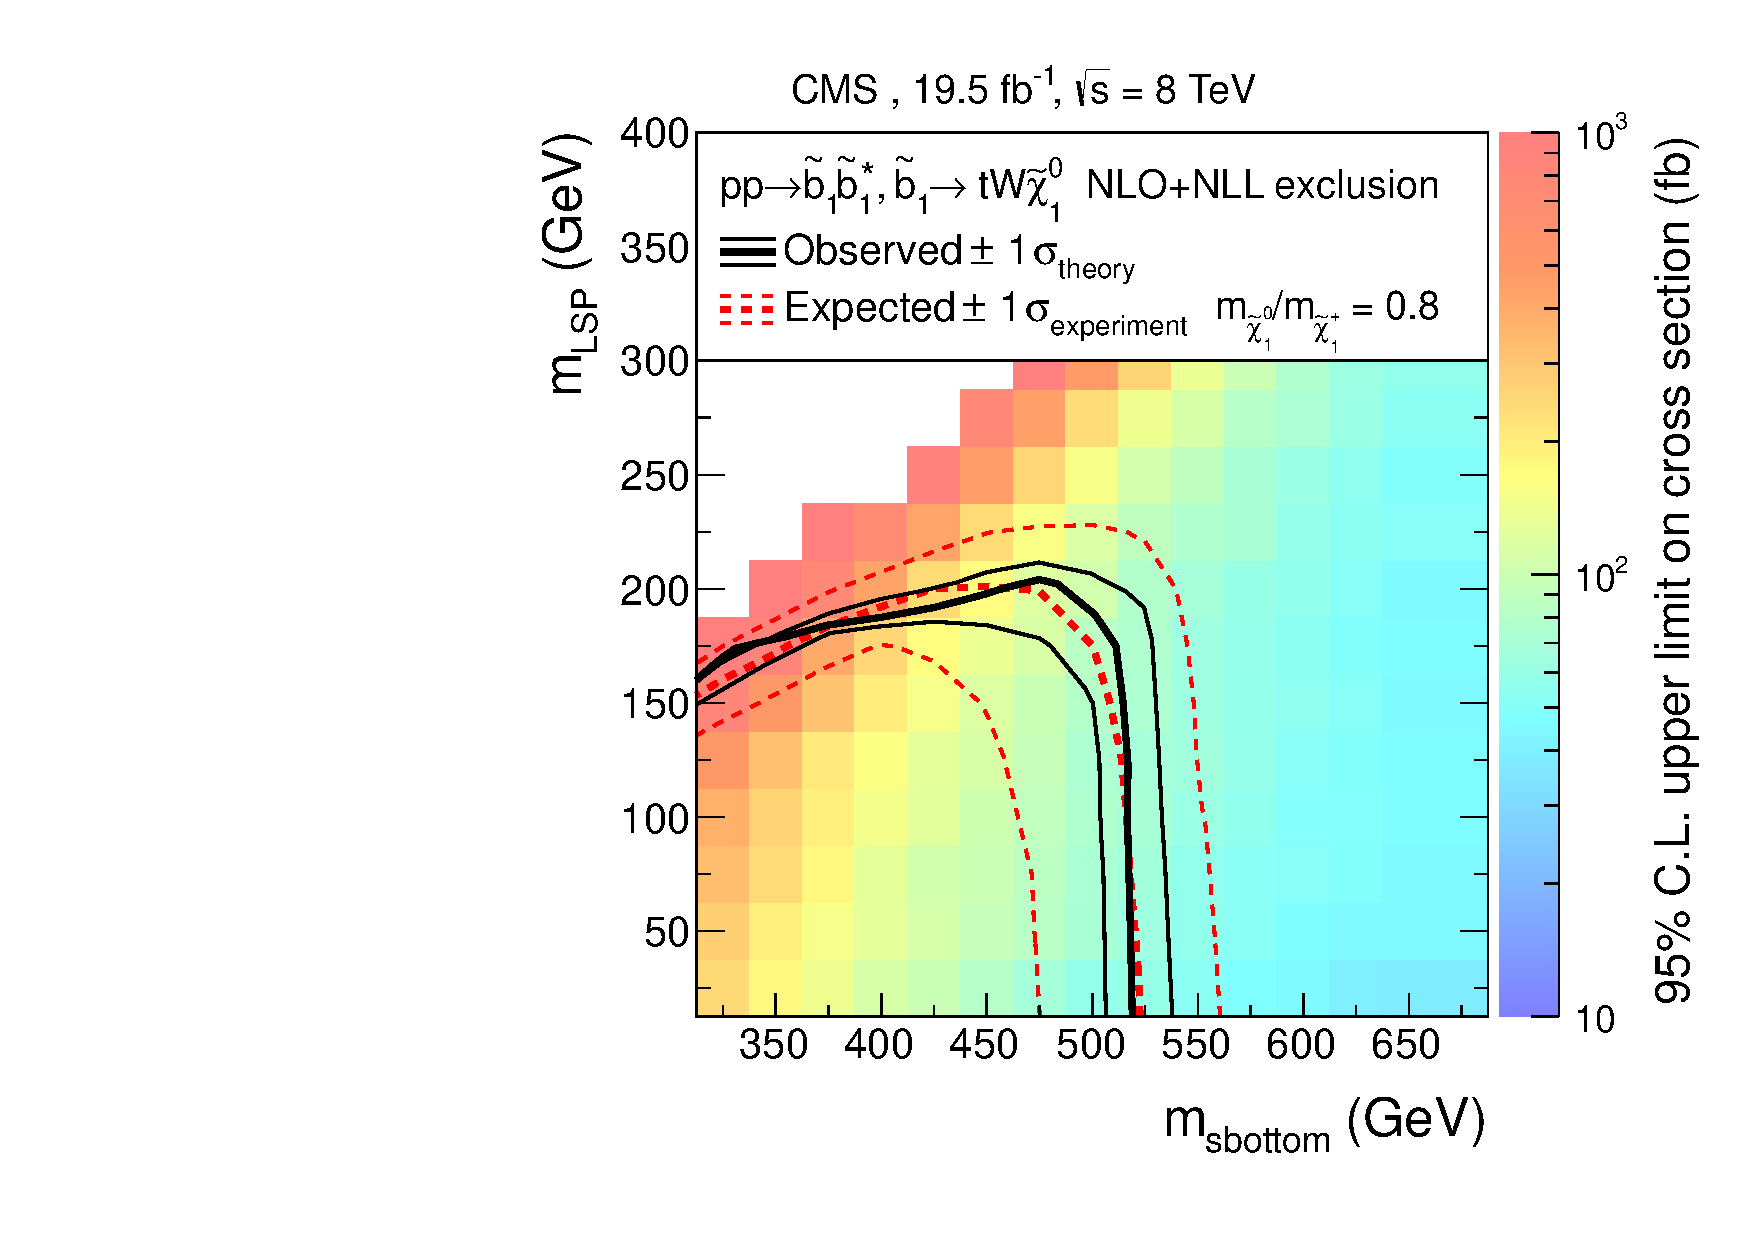
\includegraphics[width=0.49\linewidth]{p_limit_t6ttww_x08}
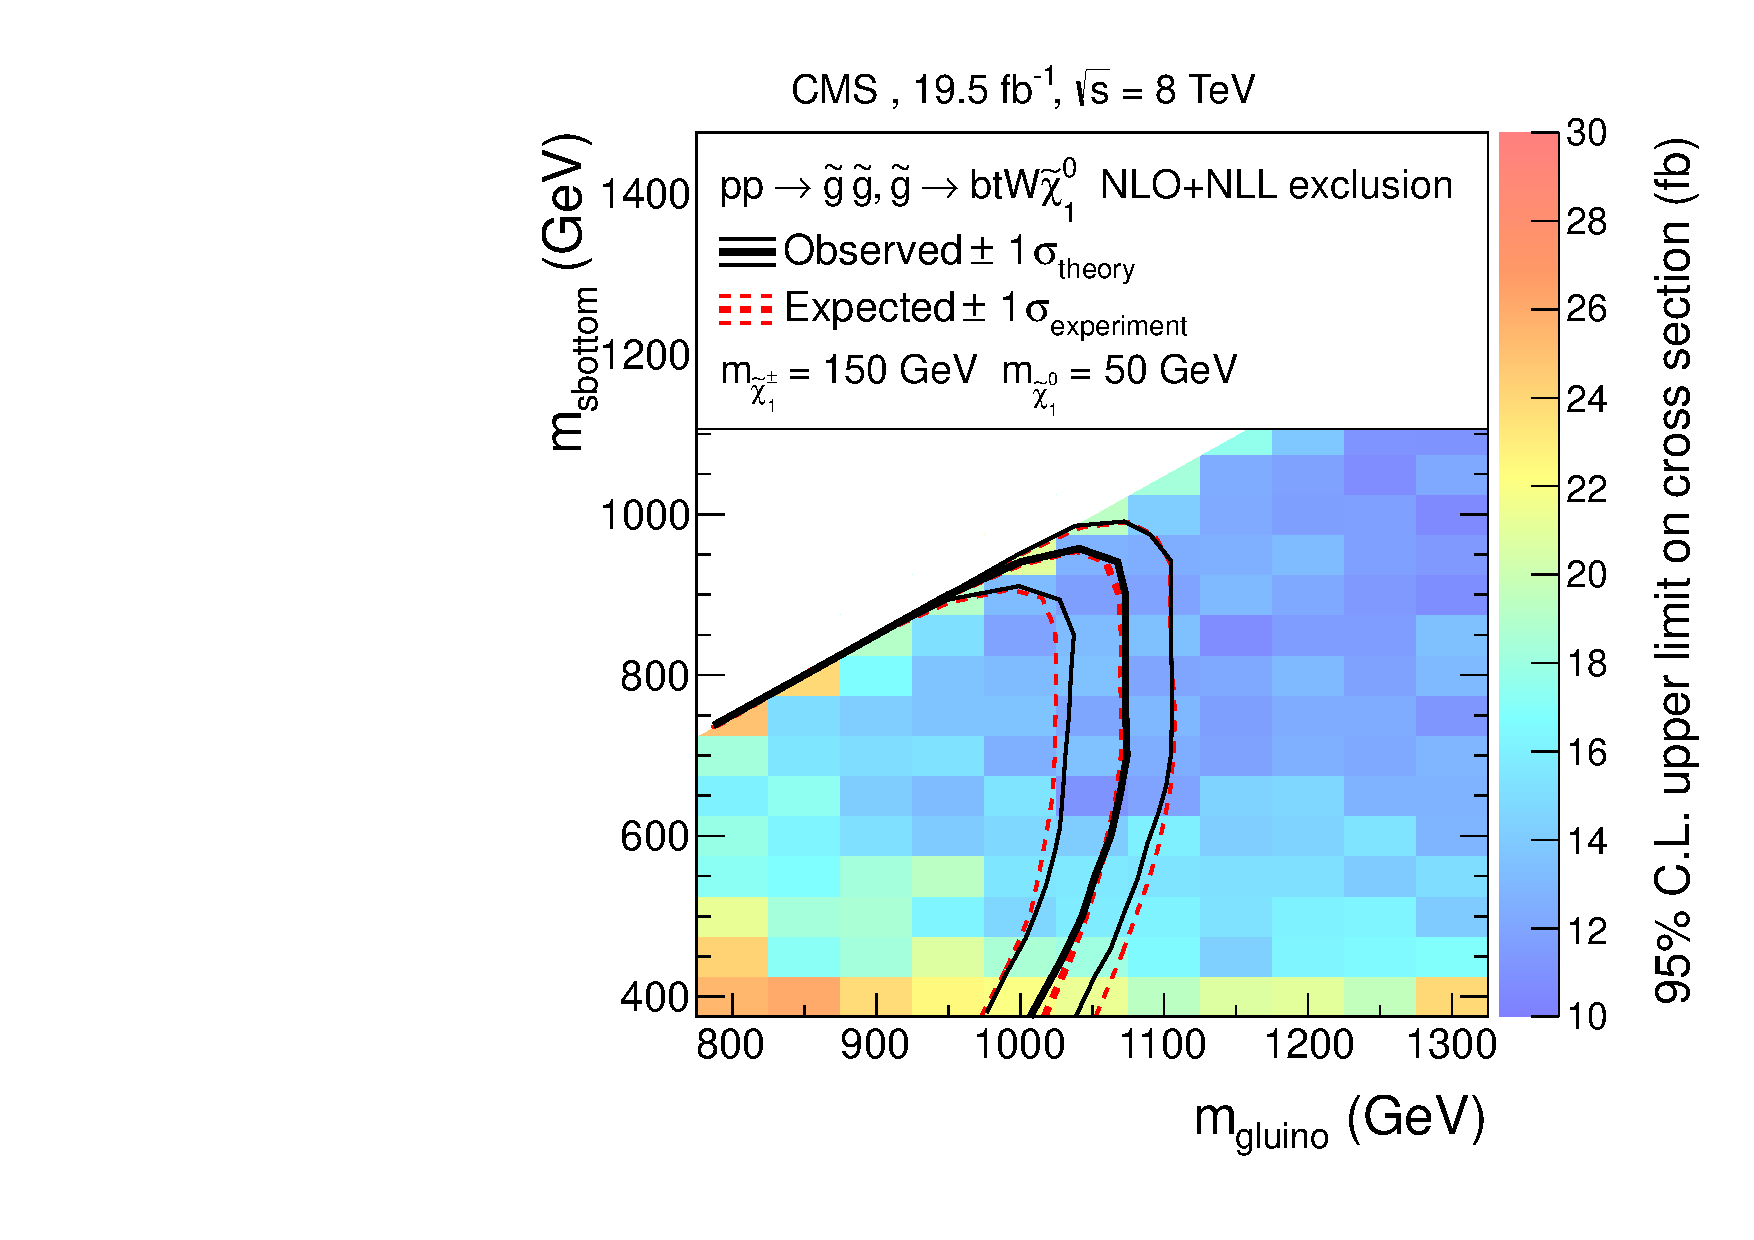
\includegraphics[width=0.49\linewidth]{p_limit_t7btw_150}
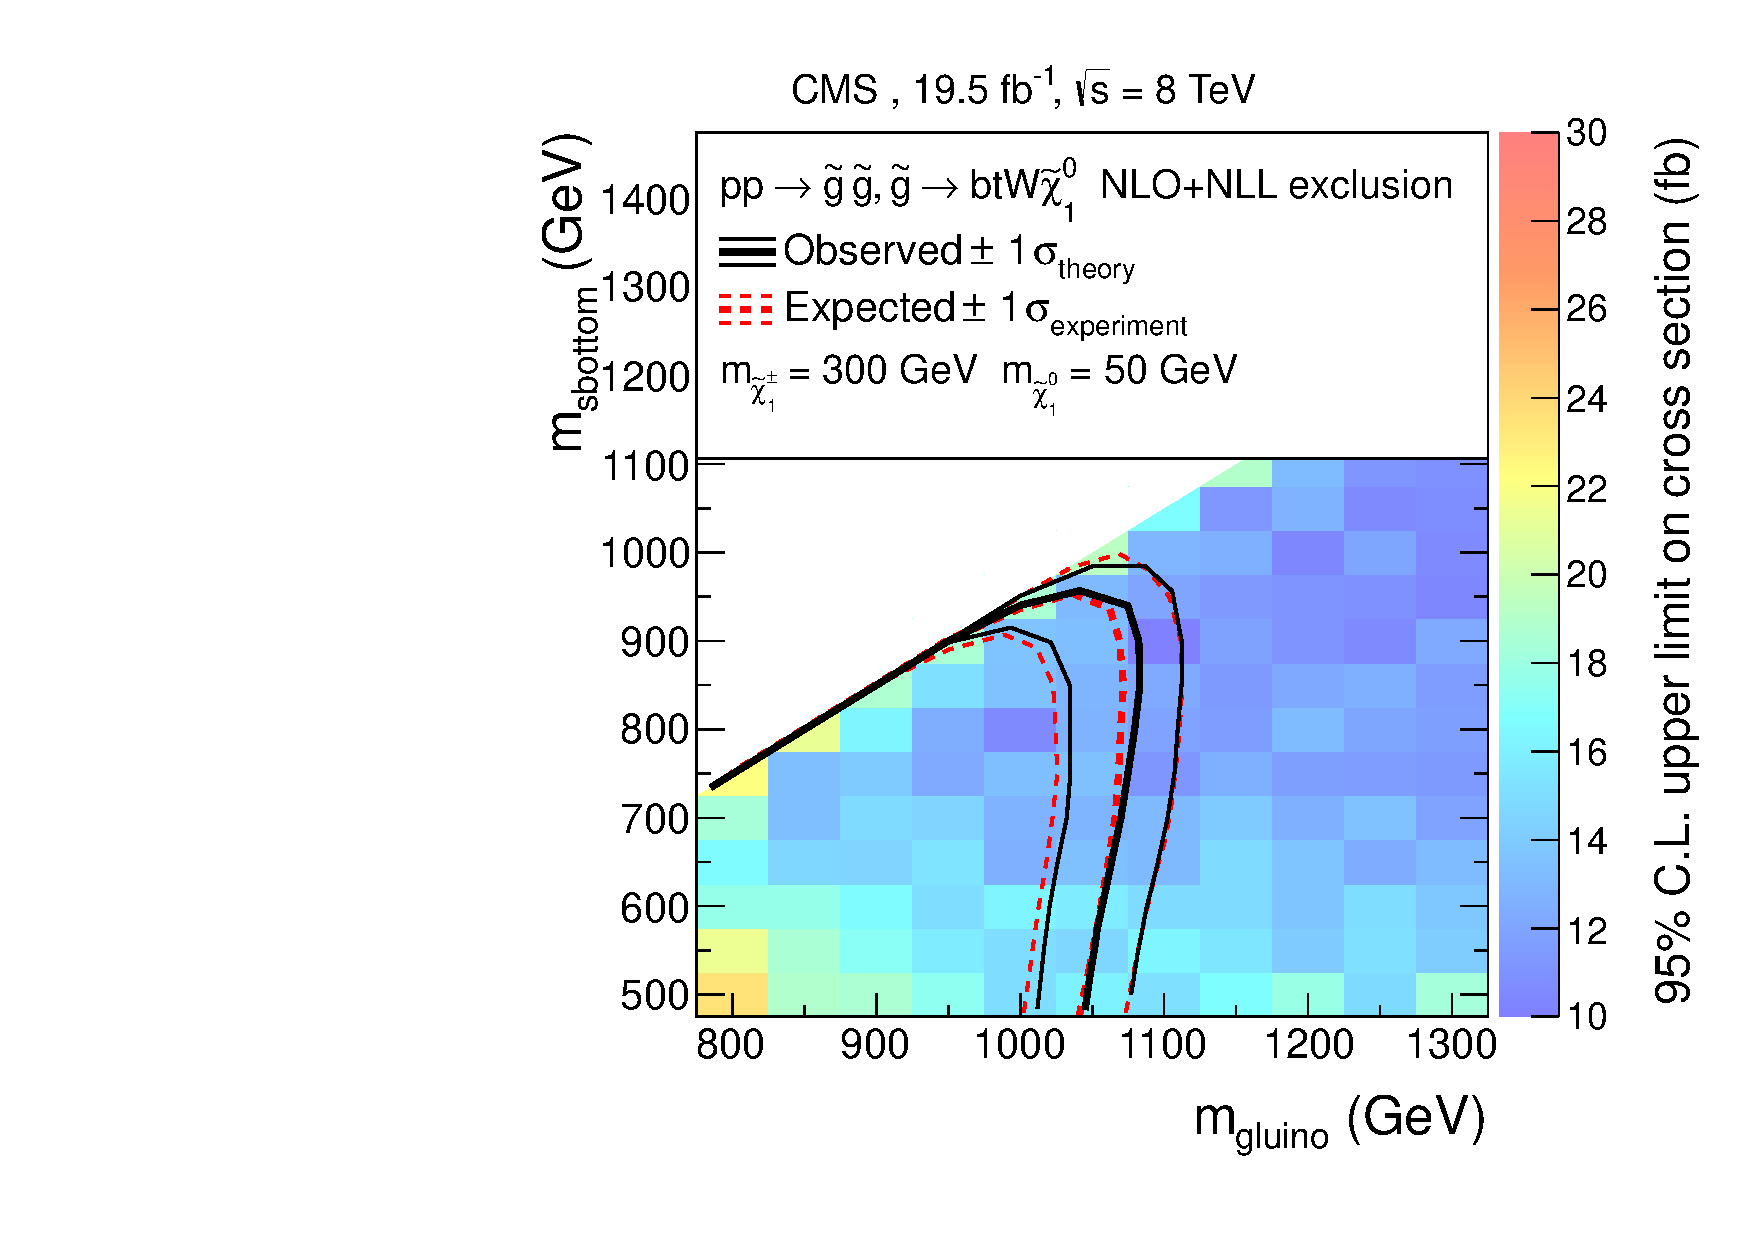
\includegraphics[width=0.49\linewidth]{p_limit_t7btw_300}
\caption[Exclusion curves for models B1 and B2]
{\label{fig:results_limit_b12}
Exclusion regions at 95\% CL in the planes of $m(\chipm_1)$ \vs $m(\sBot_1)$
and $m(\chiz_1)$ \vs $m(\sBot_1)$ (model B1) and $m(\sBot_1)$ \vs $m(\sGlu)$
(model B2). The convention for the exclusion curves are same as in
Figure~\ref{fig:results_limit_b12}.
}
\end{center}
\end{minipage}
}
\end{figure}
% --------------------------------------------------------------------------- %
\clearpage

Model C1 is another decay chain following a gluino pair production
$\Pp\Pp\to\sGlu\sGlu$, where each gluino decays to light quarks and a
chargino via a heavy virtual squark: $\sGlu\to\Pq\Paq'\chipm_1$, $\chipm_1
\to \text{W}^{(*)}\chiz_1$. The decay is charge democratic, resulting in an
equal fraction of same-sign and opposite-sign W pairs in the final state.
In this model there are three parameters: $m_{\sGlu}$, $m_{\chipm_1}$, and
$m_{\chiz_1}$. The scan is performed in the $m_{\chiz_1}$, $m_{\sGlu}$
plane, while the chargino mass is defined as $m_{\chipm_1} = xm_{\chiz_1}
+ (1-x)m_{\sGlu}$ where we examine $x$ values of 0.5 and 0.8. Depending on
the value of the $x$-parameter, for a given $m_{\chiz_1}$ and $m_{\sGlu}$,
the W can be produced on-shell or off-shell giving rise to either high-
or low-\pt leptons. In this model no enrichment of heavy-flavour jets
is expected. Therefore, the search regions SR01--SR08, with both low-
and high-\pt lepton selection, are used for cross section upper limit
calculation. In Figure~\ref{fig:results_limit_c1} we present the limit in the
$m_{\chiz_1}$--$m_{\sGlu}$ plane with $x=0.8$. In this model, gluino masses up
to 900 \GeV are probed. Most of the sensitivity for this model is obtained from
search region SR08.
% \clearpage
% --------------------------------------------------------------------------- %
\begin{figure}[!htb]
\begin{center}
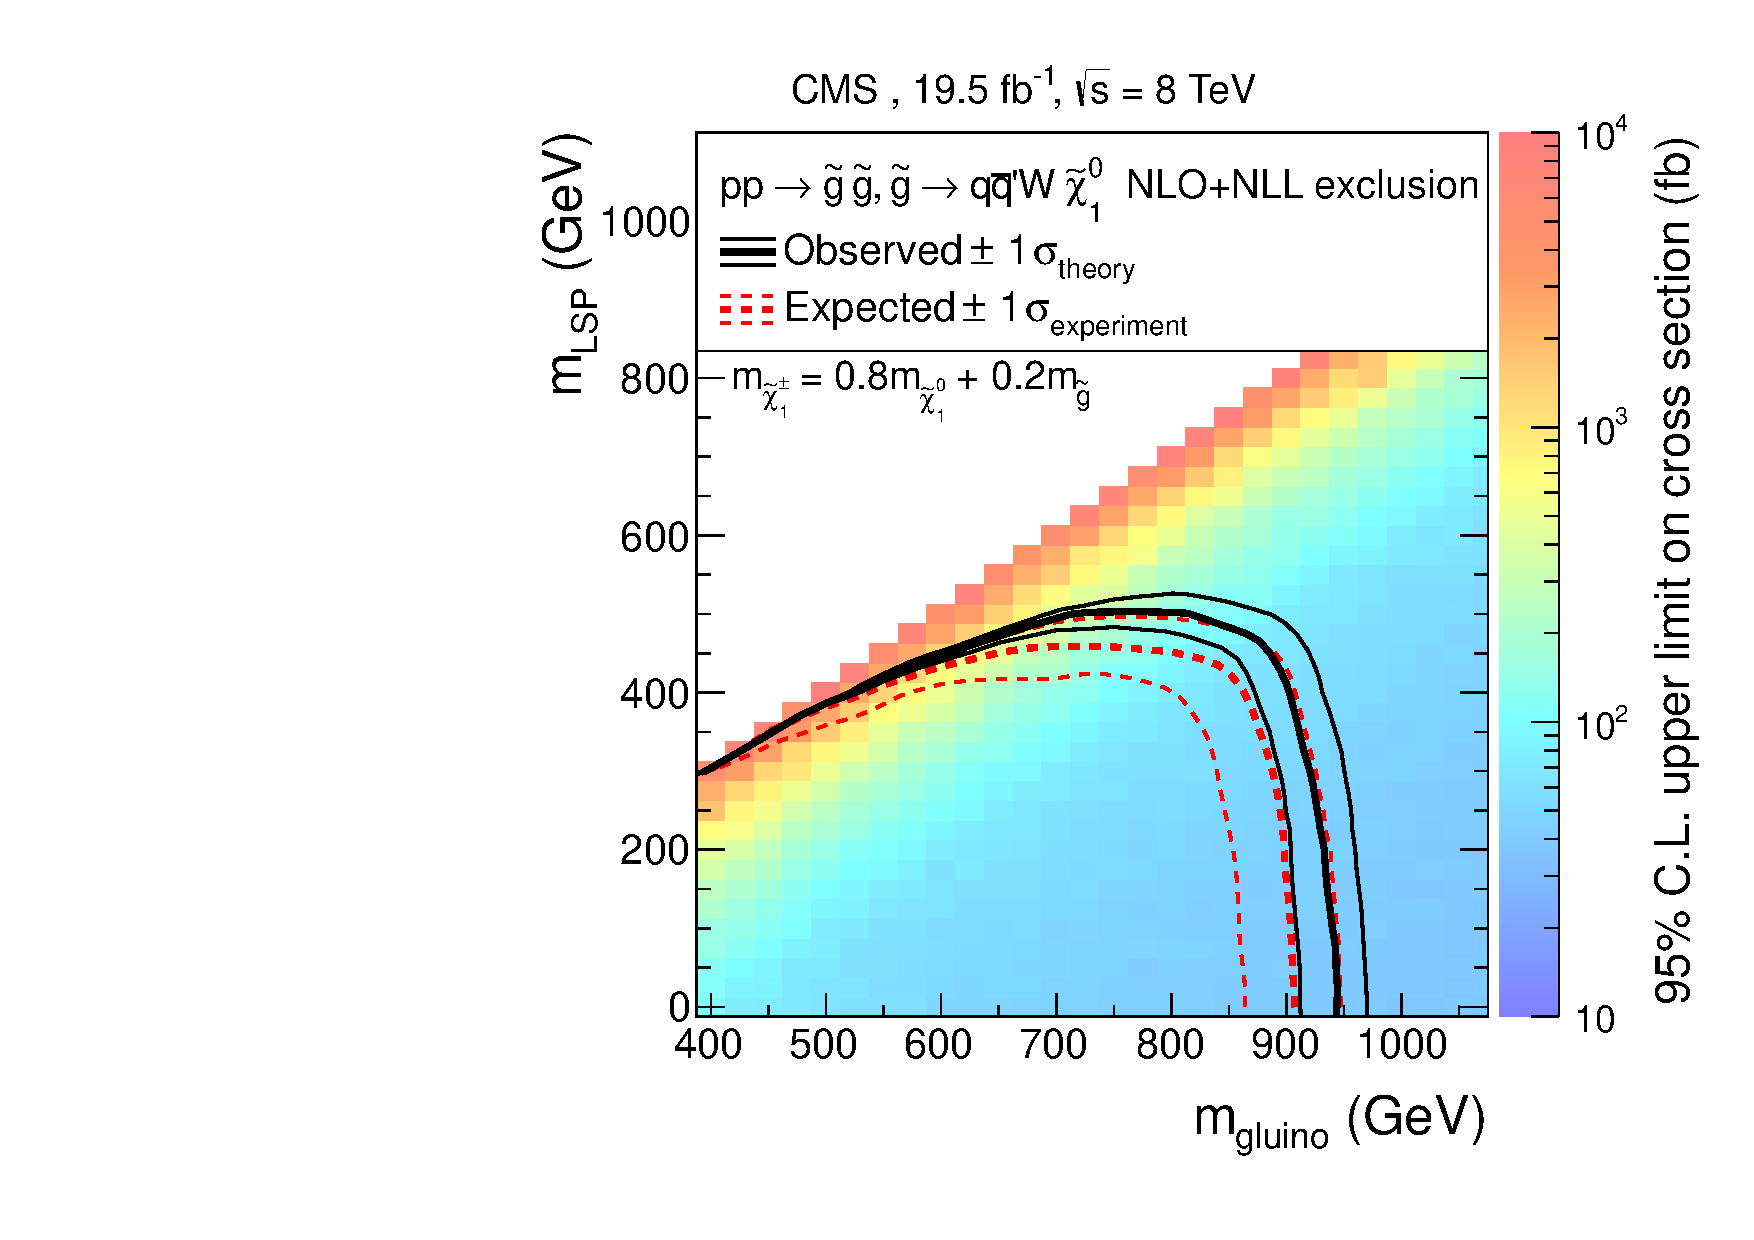
\includegraphics[width=0.49\linewidth]{p_limit_t5lnu}
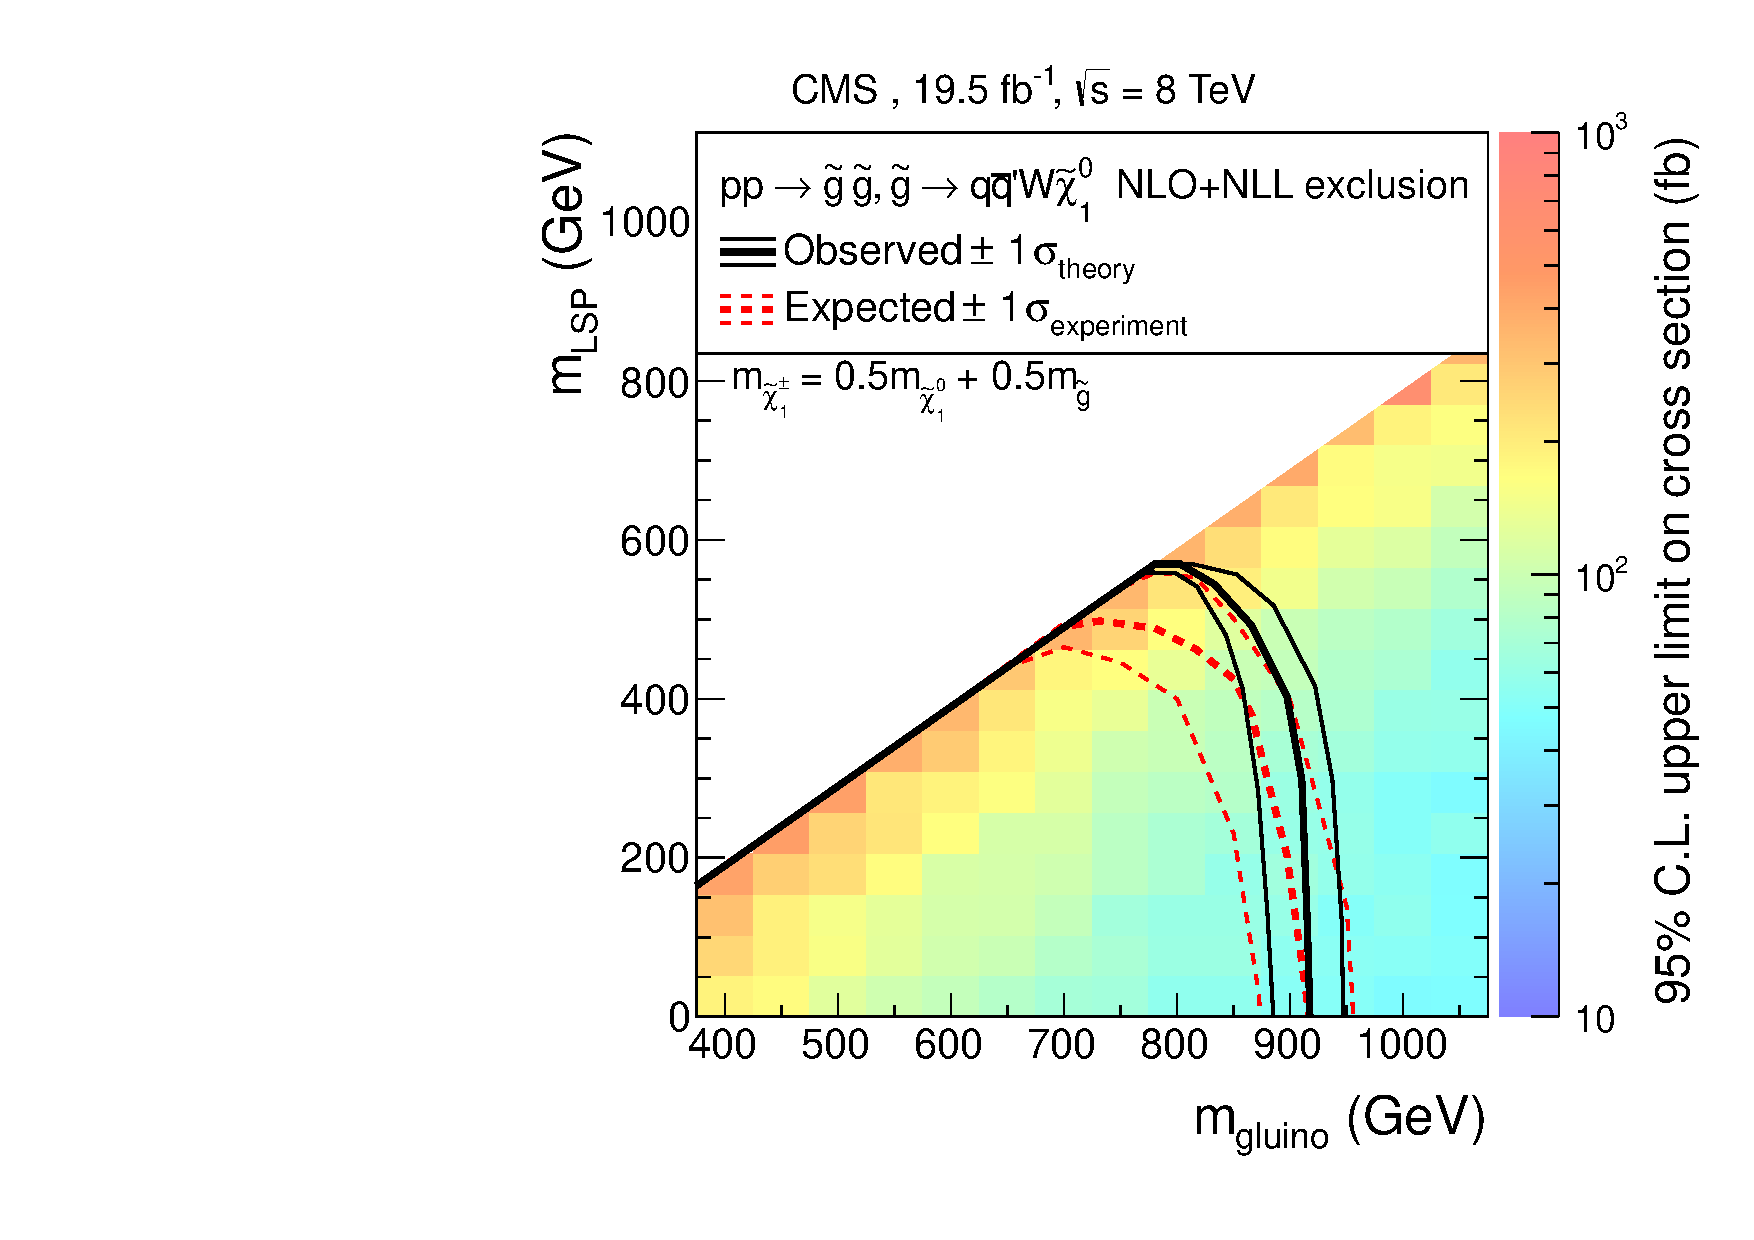
\includegraphics[width=0.49\linewidth]{p_limit_t5vv}
\caption[Exclusion curves for model C1]
{\label{fig:results_limit_c1}
Exclusion regions at 95\% CL in the planes of $m(\chiz_1)$ \vs $m(\sGlu)$
(model C1). The convention for the exclusion curves are same as in
Figure~\ref{fig:results_limit_c1}.
}
\end{center}
\end{figure}
% --------------------------------------------------------------------------- %

Excluded regions in the parameter space of the five models are shown
in Figures~\ref{fig:results_limit_a12}, \ref{fig:results_limit_b12},
and~\ref{fig:results_limit_c1}. These results extend the sensitivity obtained
in the previous version of this analysis~\cite{sspaper2012} on gluino and
sbottom masses. For the gluino-initiated models (A1, A2, B2, and C1), we probe
gluinos with masses below around 1050 \GeV, with relatively small dependence on
the details of the models. This is because the limits are driven by the common
gluino-pair production cross section. In the case of the direct bottom-squark
pair production, model B1, our search shows sensitivity for sbottom masses up
to 500 \GeV.

These models are also probed by other CMS new physics searches in
different decay modes, although other searches have so far been
interpreted in the context of model A1 but not A2, B1, or B2. For model
A1 the limits given here are complementary to the limits from other
searches~\cite{maria,Chatrchyan:2012wa,Chatrchyan:2013lya,Chatrchyan:2013wxa}:
less stringent at low $m(\chiz_1)$ but more stringent at high $m(\chiz_1)$.
A similar conclusion applies to model A2, since the final state is the same,
while in the case of bottom-squark pair production limits on $m(\sBot_1)$ are
about 500(600) \GeV, but assuming the decay mode $\sBot_1 \to \cPqb \chiz_1$
instead of the model B1 mode $\sBot_1 \to \cPqt \chim_1$~\cite{ATLAS:2011cw}.
Comparable limits for model A1, as well as for similar models with top
and bottom quarks from gluino decays, have been reported by the ATLAS
collaboration~\cite{ATLAS:2012ai,ATLAS:2012ah,ATLAS:2012pq,ATLAS:2012naa}.

One R-parity violating scenario is considered in the scope of gluino-pair
production, where each gluino decays to three quarks: $\sGlu\to\cPqt\cPqb\cPqs
(\cPaqt\cPaqb\cPaqs)$ (model RPV). Such decays lead to same-sign W pairs in
the final state in 50\% of the cases. The model is governed by one parameter
($m_{\sGlu}$) which dictates the production cross section and the final state
kinematics. The dedicated search region RPV2 with the high-$\pt$ lepton selection
is used to place an upper limit on the production cross section. The signal
selection efficiency is $0.1\%$ for low gluino masses and reaches to $0.5\%$
for the higher gluino masses considered in this analysis. The result is shown
in Figure~\ref{fig:results_limit_rpv}. In this scenario, the gluino mass is probed up to
approximately 900 \GeV.

% --------------------------------------------------------------------------- %
\begin{figure}
\begin{center}
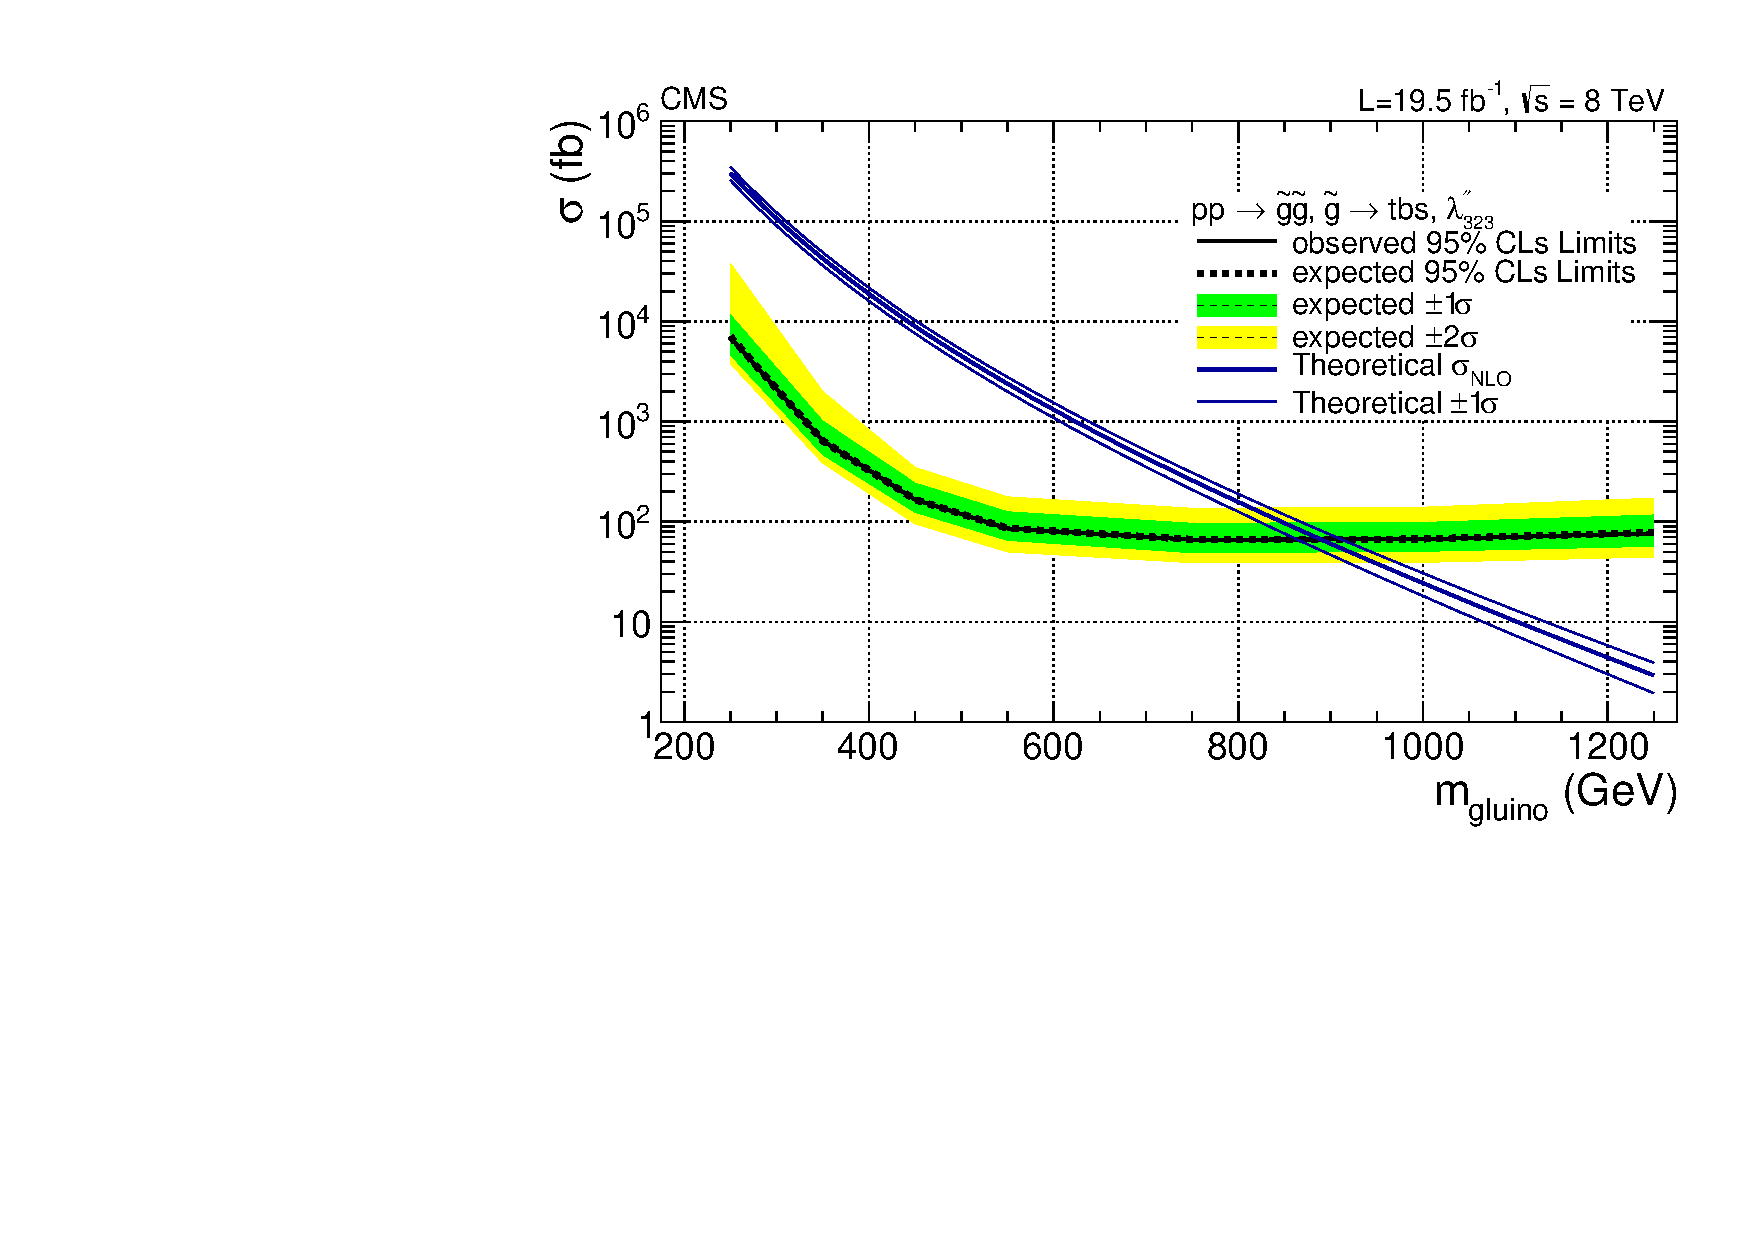
\includegraphics[width=0.60\linewidth]{p_limit_rpv.pdf}
\caption[Exclusion curve for RPV model]
{\label{fig:results_limit_rpv}
Exclusion at 95\% CL upper limit on the gluino production cross section for
an RPV simplified model, $pp \to \sGlu \sGlu, \sGlu \to \cPqt\cPqb\cPqs
(\cPaqt\cPaqb\cPaqs)$.
}
\end{center}
\end{figure}
% --------------------------------------------------------------------------- %
